\documentclass[11pt]{report} 
\usepackage{epsf}
\usepackage{graphicx}
\usepackage{index}
\usepackage{varioref}
\usepackage{amsmath}
\usepackage{multirow}
\usepackage{theorem} % for examples
\usepackage{alltt}
\usepackage{ulem}
\usepackage{epic,eepic}
\usepackage{boxedminipage}
\usepackage{fancybox}
\usepackage[square]{natbib}
\usepackage{ps4pdf}
\usepackage{picins} % pictures next to paragraphs, Ondrej's part
\usepackage{avm}
\usepackage{epsfig}
\PSforPDF{
\usepackage{dtree} % a dependency tree
\usepackage{pstricks}
\usepackage{pst-node}
\usepackage{pst-plot}
}
\usepackage{subfig}
\oddsidemargin 0mm
\evensidemargin 5mm
\topmargin -20mm
\textheight 240mm
\textwidth 160mm



\newcommand{\bold}{\it}
\renewcommand{\emph}{\it}

\makeindex
\theoremstyle{plain}

\begin{document}
\title{\vspace{-15mm}\LARGE {\bf Final Report}\\[2mm]
of the\\[2mm]
2006 Language Engineering Workshop\\[15mm]
{\huge \bf Open Source Toolkit\\[2mm]
\bf for Statistical Machine Translation:\\[5mm]
Factored Translation Models\\[2mm]
and Confusion Network Decoding}\\[10mm]
{\tt \Large http://www.clsp.jhu.edu/ws2006/groups/ossmt/}\\[2mm]
{\tt \Large http://www.statmt.org/moses/}\\[15mm]
Johns Hopkins University\\[2mm]
Center for Speech and Language Processing}
\author{\large Philipp Koehn,
Marcello Federico,
Wade Shen,
Nicola Bertoldi,\\
\large 
Ond\v{r}ej Bojar,
Chris Callison-Burch,
Brooke Cowan,
 Chris Dyer,
Hieu Hoang,
Richard Zens,\\
\large Alexandra Constantin,
Christine Corbett Moran,
Evan Herbst}
\normalsize

\maketitle
 
\section*{Abstract}
The 2006 Language Engineering Workshop {\bold Open Source Toolkit for Statistical Machine Translation} had the objective to advance the current state-of-the-art in statistical machine translation through richer input and richer annotation of the training data. The workshop focused on three topics: factored translation models, confusion network decoding, and the development of an open source toolkit that incorporates this advancements.

This report describes the scientific goals, the novel methods, and experimental results of the workshop. It also documents details of the implementation of the open source toolkit.

\phantom{.}


\newpage
\section*{Acknowledgments}
The participants at the workshop would like to thank everybody at Johns Hopkins University who made the summer workshop such a memorable --- and in our view very successful --- event. The JHU Summer Workshop is a great venue to bring together researchers from various backgrounds and focus their minds on a problem, leading to intense collaboration that would not have been possible otherwise.

We especially would like to thank Fred Jelinek for heading the Summer School effort and Laura Graham and Sue Porterfield for keeping us sane during the hot summer weeks in Baltimore.

Besides the funding acquired from JHU for this workshop from DARPA and NSF, the participation at the workshop was also financially supported by the funding by the GALE program of the Defense Advanced Research Projects Agency, Contract No. HR0011-06-C-0022 and funding by the University of Maryland, the University of Edinburgh and MIT Lincoln Labs\footnote{This work was sponsored by the Department of Defense under Air Force Contract FA8721-05-C-0002. Opinions, interpretations, conclusions, and recommendations are those of the authors and are not necessarily endorsed by the United States Government.}.

\phantom{.}

\newpage
\section*{Team Members}

\begin{itemize}
\item Philipp Koehn, Team Leader, University of Edinburgh
\item Marcello Federico, Senior Researcher, ITC-IRST
\item Wade Shen, Senior Researcher, Lincoln Labs
\item Nicola Bertoldi, Senior Researcher, ITC-IRST
\item Ond\v{r}ej Bojar, Graduate Student, Charles University
\item Chris Callison-Burch, \sout{Graduate Student, University of Edinburgh}\\ 
\phantom{.} \hspace{1.35in}  Assistant Research Professor, JHU 
\item Brooke Cowan, Graduate Student, MIT
\item Chris Dyer, Graduate Student, University of Maryland
\item Hieu Hoang, Graduate Student, University of Edinburgh
\item Richard Zens, Graduate Student, RWTH Aachen University
\item Alexandra Constantin, Undergraduate Student, Williams College
\item Evan Herbst, Undergraduate Student, Cornell
\item Christine Corbett Moran, Undergraduate Student, MIT
\end{itemize}
\tableofcontents

\chapter{Introduction}
Statistical machine translation has emerged as the dominant paradigm in machine translation research.  Statistical machine translation is built on the insight that many translation choices have to be weighed against each other --- whether it is different ways of translating an ambiguous word, or alternative ways of reordering the words in an input sentence to reflect the target language word order.  In statistical machine translation these choices are guided using probabilities which are estimated using collections of translated texts, called parallel corpora.  

While statistical machine translation research has gained much by building on the insight that probabilities may be used to make informed choices, current models are deficient because they lack crucial information.  Much of the translation process is best explained with morphological, syntactic, semantic, or other information that is not typically contained in parallel corpora.  We show that when such information is incorporated to the training data, we can build richer models of translation, which we call {\bf factored translation models}.  Since we automatically tag our data there often many ways of marking up input sentences.  This further increases multitude of choices that our machine translation must deal with, and requires an efficient method for dealing with potentially ambiguous input.    We investigate {\bf confusion network decoding} as a way of addressing this challenge.   

In addition to these scientific goals, we also address another pervasive problem for our field.  Given that the methods and systems we develop are increasingly complex, simply catching up with the state-of-the-art has become a major part of the work done by research groups. To reduce this tremendous duplication of efforts, we have made our work available in an {\bf open source toolkit}. To this end, we merged the efforts of a number of research labs (University of Edinburgh, ITC-irst, MIT, University of Maryland, RWTH Aachen) into a common set of tools, which includes the core of a machine translation system: the decoder. This report documents this effort, which we have continued to pursue beyond the summer workshop.

\section{Factored Translation Models}
We are proposing a new approach that we call factored translation models, which extends traditional phrase-based statistical machine translation models to take advantage from additional annotation, especially linguistic markup.  Phrase-based statistical machine translation is a very strong baseline to improve upon. Phrase-based systems have consistently outperformed other methods in recent competitions. Any improvements over this approach therefore implies an improvement in the state-of-the-art.

The basic idea behind factored translation models is to represent phrases not simply as sequences of fully inflected words, but instead as sequences containing multiple levels of information.  A word in our model is not a single token, but vector of factors. This enables straight-forward integration of part-of-speech tags, morphological information, and even shallow syntax.  Instead of dealing with linguistic markup in preprocessing or postprocessing steps (e.g., the re-ranking approaches of the 2003 JHU workshop), we build a system that intergrate this information into the decoding process to better guide the search.

Our approach to factored translation models is described in detail in Chapter~\ref{chap:factored-models}.  The results of the experiments that we conducted on factored translation between English and German, Spanish and Czech are given in Chapter~\ref{chap:factored-experiments}.

\section{Confusion Network Decoding}

With the move to factored translation models, there are now several reasons why we may have to deal with ambiguous input. One is that the tools that we use to annotated our data may not make deterministic decisions. Instead of only relying on the 1-best output of our tools, we accept ambiguous input in the form of confusion networks.  This preserves ambiguity and defers firm decisions until later stages, which has been shown to be advantageous in previous research.  

While confusion networks are a useful way of dealing with ambiguous factors, they are more commonly used to represent the output of automatic speech recognition when combining machine translation and speech recognition in speech translation systems.  
Our approach to confusion network decoding, and its application to speech translation, is described in detail in Chapter~\ref{chap:confusion-networks}.  Chapter \ref{confusion-net-experiments} presents experimental results using confusion networks.  

\section{Open Source Toolkit}
There are several reasons to create an open research environment by opening up resources (tools and corpora) freely to the wider community. Since our research is largely publicly funded, it seems appropriate to return the products of this work to the public. Access to free resources enables other research group to advance work that was started here, and provides them with baseline performance results for their own novel efforts.

While these are honorable goals, our motivation for creating this toolkit is also somewhat self-interested: Building statistical machine translation systems has become a very complex task, and rapid progress in the field forces us to spend much time reimplementing other researchers' advances in our system. By bringing several research groups together to work on the same system, this duplication of effort is reduced and we can spend more time on what we would really like to do: Come up with new ideas and test them.

The starting point of the Moses system was the Pharaoh system of the University of Edinburgh \citep{koe:04}.  It was re-engineered during the workshop, and several major new components were added. Moses is a full-fledged statistical machine translation system, including the training, tuning and decoding components. The system provides state-of-the-art performance out of the box, as has been shown at recent ACL-WMT \citep{callisonburch-EtAl:2007:WMT}, TC-STAR, and IWSLT \citep{ShenIWSLT} evaluation campaigns.

The implementation and usage of the toolkit is described in more detail in Chapter~\ref{toolkit}.

\chapter{Factored Translation Models}\label{chap:factored-models}

The current state-of-the-art approach to statistical machine translation, so-called phrase-based models, represent phrases as sequences of words without any explicit use of linguistic information, be it morphological, syntactic, or semantic. Such information has been shown to be valuable when it is integrated into pre-processing or post-processing steps.   For instance, improvements in translation quality have been achieved by preprocessing Arabic morphology through stemming or splitting off of affixes that typically translate into individual words in English \citep{Habash2005}.  Other research shows the benefits of reordering words in German sentences prior to translation so that their word order is more similar to English word order \citep{Collins2005}.

However, a tighter integration of linguistic information into the translation model is desirable for two reasons:
\begin{itemize}
\item Translation models that operate on more general representations, such as lemmas instead of surface forms of words, can draw on richer statistics and overcome data sparseness problems caused by limited training data.
\item Many aspects of translation can be best explained on a morphological, syntactic, or semantic level. Having such information available to the translation model allows the direct modeling of these aspects. For instance: reordering at the sentence level is mostly driven by general syntactic principles, local agreement constraints show up in morphology, etc.
\end{itemize}

Therefore, we developed a framework for statistical translation models that tightly integrates additional information. Our framework is an extension of phrase-based machine translation \citep{OchThesis}. 


\section{Current Phrase-Based Models}


\begin{figure}
\begin{center}
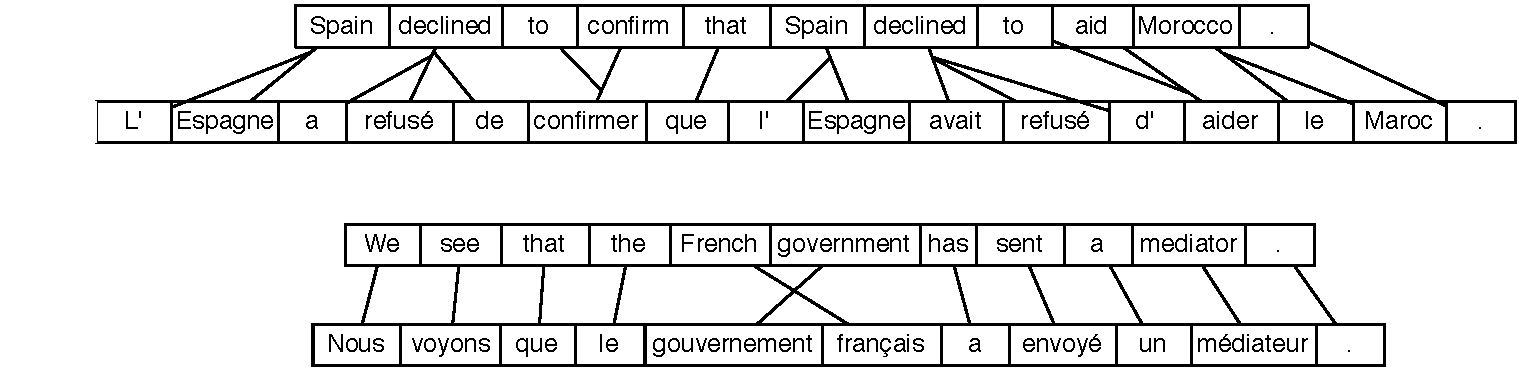
\includegraphics[width=\linewidth]{images/word-aligned-parallel-corpus}
\end{center}
\caption{Word-level alignments are generated for sentence pairs using the IBM Models.}\label{word-aligned-parallel-corpus}
\end{figure}



Current phrase-based models of statistical machine translation \citep{OchThesis, koe:03} are based on on earlier word-based models \citep{Brown1988,Brown1993} that define the translation model probability $P(\mathbf{f} | \mathbf{e})$ in terms of word-level alignments $\mathbf{a}$.  
\begin{equation}
P(\mathbf{f} | \mathbf{e}) = \sum_a{P(\mathbf{a},\mathbf{f} | \mathbf{e})}\label{conditional-probability-as-sum-over-alignments}
\end{equation}
\citet{Brown1993} introduced a series of models, referred to as the IBM Models, which defined the alignment probability $P(\mathbf{a},\mathbf{f} | \mathbf{e})$ so that its parameters could be estimated from a parallel corpus using expectation maximization.  



Phrase-based statistical machine translation uses the IBM Models to create high probability word-alignments, such as those shown in Figure \ref{word-aligned-parallel-corpus}, for each sentence pair in a parallel corpus.  All phrase-level alignments that are consistent with the word-level alignments are then enumerated using phrase-extraction techniques \citep{Marcu2002,koe:03,Tillmann2003,Venugopal2003}. 
This is illustrated in Figure \ref{phrase-extraction}.  The highlighted regions show how two French translations of the English phrase {\it Spain declined} can be extracted using the word alignment. Once they have been enumerated these phrase-level alignments are used to estimate a {\it phrase translation probability}, $p(\bar{f} | \bar{e})$, between a foreign phrase $\bar{f}$ and English phrase $\bar{e}$.  This probability is generally estimated using maximum likelihood as
%
\begin{equation}
p(\bar{f} | \bar{e})  = \frac{count(\bar{f}, \bar{e})}{count(\bar{e})}\label{phrase-translation-probability}
\end{equation}
%
\begin{figure}
\begin{center}
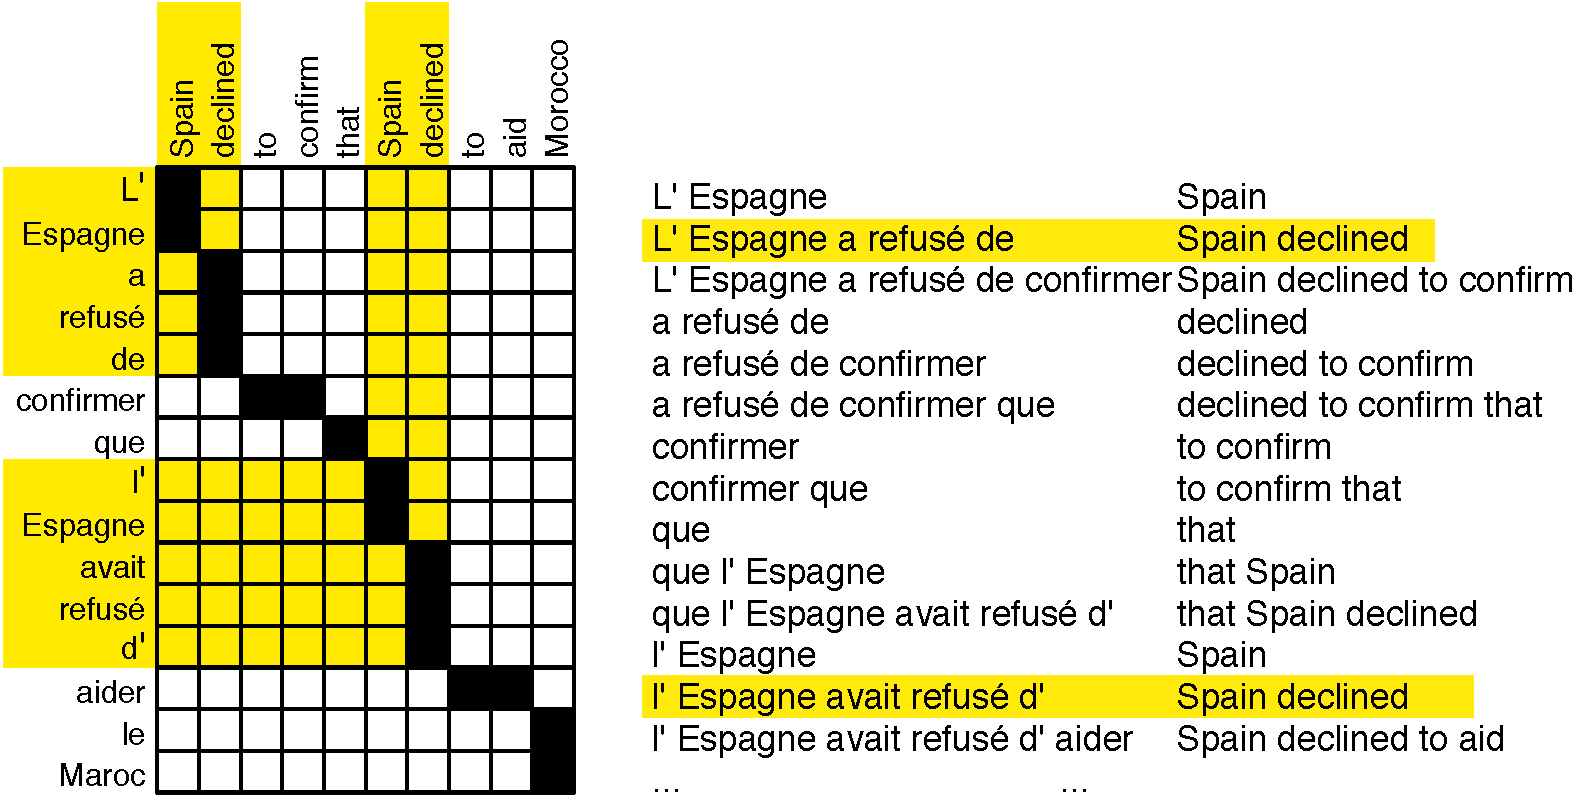
\includegraphics[scale=.55]{images/phrase-extraction}
\end{center}
\caption{Phrase-to-phrase correspondences are enumerated from word-level alignments.}\label{phrase-extraction}
\end{figure}
%
The phrase translation probability is integrated into a log linear formulation of translation \citep{Och2002}.  The log linear formulation of translation is given by
\begin{equation}
P(\mathbf{e} | \mathbf{f}) = \exp \sum_{i=1}^{n}{\lambda_i h_i (\mathbf{e}, \mathbf{f})} \label{log-linear-formulation}
\end{equation}
%
Where  $h_i$ can be an arbitrary {\it feature function} that assigns a score to a  translation.  Commonly used feature functions include the phrase translation probability, and also trigram language model probabilities, word translation probabilities, phrase length penalty, and reordering costs.  




\subsection{Problems with phrase-based models}

The limitations of current approaches to statistical machine translation stem from their formulation of phrases.  Because they treat phrases as sequences of fully-inflected words and do not incorporate any additional linguistic information, they are limited in the following ways:
\begin{itemize}
\item They are unable to learn translations of words that do not occur in the data, because they are unable to generalize.  Current approaches know nothing of  morphology, and fail to connect different word forms.  When a form of a word does not occur in the training data, current systems are unable to translate it.  This problem is severe for languages which are highly inflective, and in cases where only small amounts of training data are available. 
\item They are unable to distinguish between different linguistic contexts.  When current models have learned multiple possible translations for a particular word or phrase, the choice of which translation to use is guided by frequency information rather than by linguistic information.   Often times linguistic factors like case, tense, or agreement are important determinants  for what translation ought to be used in a particular context.  Because current phrase-based approaches lack linguistic information they do not have an  appropriate means of choosing between alternative translations.  
\item They have limited capacities for learning linguistic facts.   Because current models do not use any level of abstraction above words, it is impossible to model simple linguistic facts.  Under current approaches it is impossible to learn or to explicitly specify that adjective-noun alternation occurs between two languages, or that a language's word order is subject-object-verb, or similar linguistic facts.  
\end{itemize}


\section{Factored Translation Models}

\begin{figure}
\begin{center}
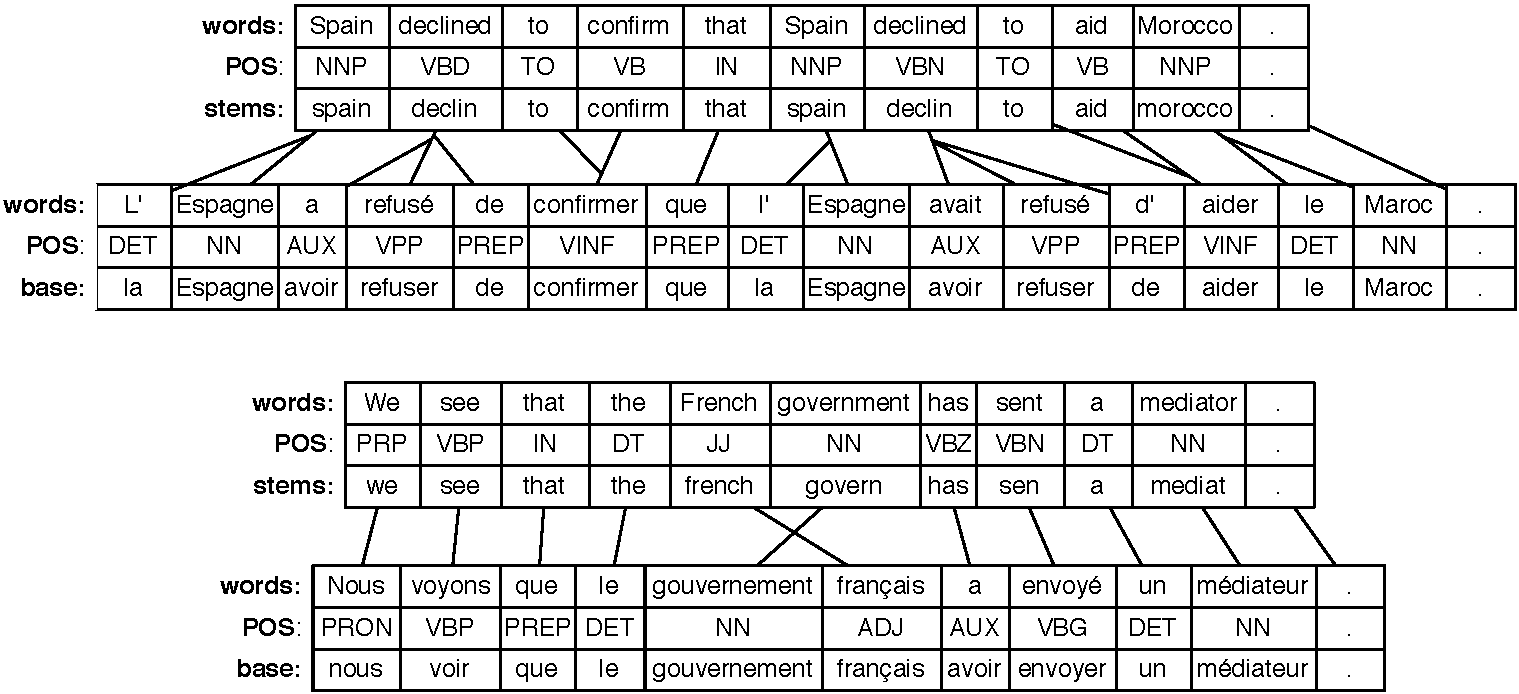
\includegraphics[width=\linewidth]{images/word-aligned-parallel-corpus-plus-factors}
\end{center}
\caption{Factored Translation Models integrate multiple levels of information in the training data.}\label{word-aligned-parallel-corpus-plus-factors}
\end{figure}

We propose Factored Translation Models to advance statistical machine translation through the incorporation multiple levels of information.  These layers of information, or {\it factors}, are integrated into both the training data and the models.  The parallel corpora used to train Factored Translation Models are tagged with factors such as parts of speech and lemmas, as shown in Figure \ref{word-aligned-parallel-corpus-plus-factors}.   Instead of modeling translation between full inflected words in the source and targets, our models can incorporate more general mappings between factors in the source and target (and between factors within the target, as well shall shortly discuss).  We can represent different models graphically by showing the mappings between the different factors, by adding connecting lines in Figure \ref{graphical-model}.



\begin{figure}
\begin{center}
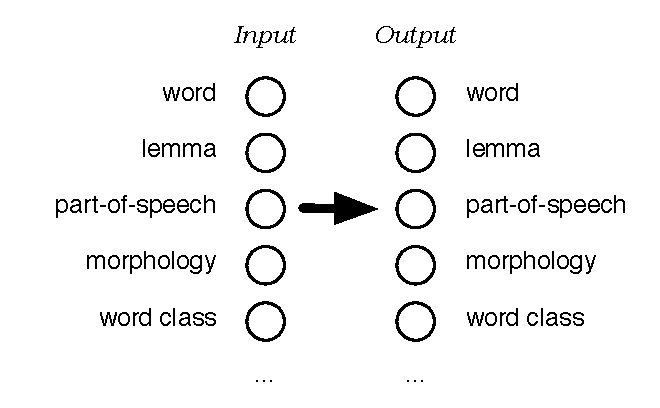
\includegraphics[scale=0.75]{factors.pdf}
\end{center}
\caption{The models specify a mapping between factors in the source and target languages.  In this report we represent different model configurations by showing which factors are connected using arrows.}\label{graphical-model}
\end{figure}


The use of factors introduces several advantages over current phrase-based approaches:
\begin{itemize}
\item Morphology can be better handled by translating in multiple steps.
\item Linguistic context can facilitate better decisions when selecting among translations.   
\item Linguistic mark up of the training data allows for many new modeling possibilities. 
\end{itemize}

\subsection{Better handling of morphology}

One example of the short-comings of the traditional surface word approach in statistical machine translation is the poor handling of morphology. Each word form is treated as a token in itself. This means that the translation model treats, say, the word {\bold house} as  completely independent of the word {\bold houses}. Any instance of {\bold house} in the training data does not add any knowledge to the translation of {\bold houses}. 

In the extreme case, while the translation of {\bold house} may be known to the model, the word {\bold houses} may be unknown and the system will not be able to translate it. While this problem does not show up as strongly in English --- due to the very limited morphological production in English --- it does constitute a significant problem for morphologically rich languages such as Arabic, German, Czech, etc.

Thus, it may be preferable to model translation between morphologically rich languages on the level of lemmas, and thus pooling the evidence for different word forms that derive from a common lemma. In such a model, we would want to translate lemma and morphological information separately,\footnote{Note that while we illustrate the use of factored translation models on such a linguistically motivated example, our framework can be equally well applied to models that incorporate automatically defined word classes.} and combine this information on the target side to generate the ultimate output surface words.  Such a model, which makes more efficient use of the translation lexicon, can be defined as a factored translation model as illustrated in Figure \ref{mophology-example}.

\begin{figure}
\begin{center}
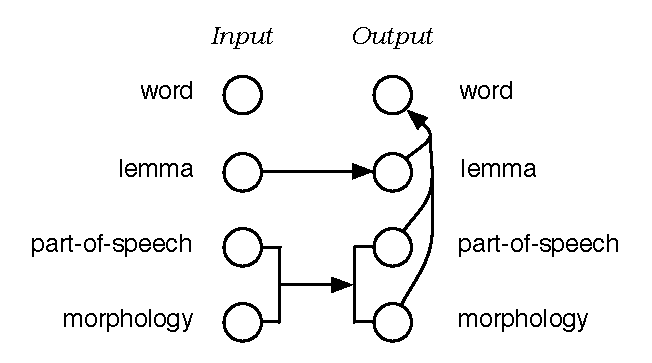
\includegraphics[scale=0.75]{factored-morphgen-symmetric.pdf}
\end{center}
\caption{A particular configuration of a factored translation model which employs {\it translation steps} between lemmas and POS+morphology, and a {\it generation step} from the POS+morphology and lemma to the fully inflected word}\label{mophology-example}
\end{figure}



\subsubsection*{Translation and Generation Steps}\label{sec:factored-decomposition}
The translation of the factored representation of source words into the factored representation of target words is broken up into a sequence of {\bf mapping steps} that either {\bf translate} input factors into output factors, or {\bf generate} additional target factors from existing target factors.

The previous of a factored model which uses morphological analysis and generation breaks up the translation process into the following steps: \vspace{-3pt}
{
\begin{itemize}\itemsep=-3pt
\item Translating morphological and syntactic factors
\item Generating surface forms given the lemma and linguistic factors
\end{itemize}
}

Factored translation models build on the phrase-based approach, which divides a sentence into small text chunks (so-called phrases) and translates those chunks. This model implicitly defines a segmentation of the input and output sentences into such phrases, such as:

\begin{center}
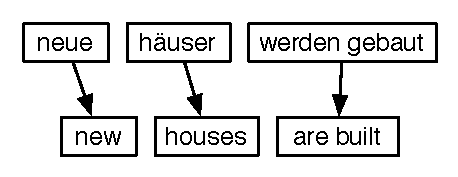
\includegraphics[scale=0.75]{phrase-model-houses.pdf}
\end{center}

Our current implementation of factored translation models strictly follows the phrase-based approach, with the additional decomposition of phrase translation into a sequence of mapping steps. Since all mapping steps operate on the same phrase segmentation of the input and output sentence into phrase pairs, we call these {\bf synchronous factored models}. 

Let us now take a closer look at one example, the translation of the one-word phrase {\bold h{\"a}user} into English. The representation of {\bold h{\"a}user} in German is: surface-form {\bold h{\"a}user}, lemma {\bold haus}, part-of-speech {\bold NN}, count {\bold plural}, case {\bold nominative}, gender {\bold neutral}. 

Given the three mapping steps in our morphological analysis and generation model may provide the following applicable mappings:
\begin{itemize}
\item {\bf Translation:} Mapping lemmas
\begin{itemize}
\item {\bold haus $\rightarrow$ house, home, building, shell}
\end{itemize}
\item {\bf Translation:} Mapping morphology
\begin{itemize}
\item {\bold NN$|$plural-nominative-neutral $\rightarrow$ NN$|$plural, NN$|$singular} 
\end{itemize}
\item {\bf Generation:} Generating surface forms
\begin{itemize}
\item {\bold house$|$NN$|$plural $\rightarrow$ houses} 
\item {\bold house$|$NN$|$singular $\rightarrow$ house} 
\item {\bold home$|$NN$|$plural $\rightarrow$ homes} 
\item {\bold ...}
\end{itemize}
\end{itemize}

The German {\bold haus$|$NN$|$plural$|$nominative$|$neutral} is expanded as follows:
\begin{itemize}
\item {\bf Translation:} Mapping lemmas\\
{\bold \{ ?$|$house$|$?$|$?,$\;\;$ ?$|$home$|$?$|$?,$\;\;$ ?$|$building$|$?$|$?,$\;\;$ ?$|$shell$|$?$|$? \}}
\item {\bf Translation:} Mapping morphology\\
{\bold \{ ?$|$house$|$NN$|$plural,$\;\;$ ?$|$home$|$NN$|$plural,$\;\;$ ?$|$building$|$NN$|$plural,$\;\;$ ?$|$shell$|$NN$|$plural,$\;\;$ ?$|$house$|$NN$|$singular,$\;\;$ ...~\}}
\item {\bf Generation:} Generating surface forms\\
{\bold \{ houses$|$house$|$NN$|$plural,$\;\;$ homes$|$home$|$NN$|$plural,$\;\;$ buildings$|$building$|$NN$|$plural,$\\ $shells$|$shell$|$NN$|$plural,$\;\;$ house$|$house$|$NN$|$singular,$\;\;$ ...~\}}
\end{itemize}

These steps are not limited to single words, but instead can be applied to sequences of factors.  Moreover, each of these steps has a probabilistic definition.  Just as phrase-based models calculate phrase translation probabilities  $p(\bar{e}_{words} | \bar{f}_{words})$ over fully inflected words, factored translation models use probabilities over more abstract features, such as $p(\bar{e}_{lemma} | \bar{f}_{lemma})$ and  $p(\bar{e}_{morph+pos} | \bar{f}_{morph+pos})$.  The generation steps can also be defined probabilistically as $p(\bar{e}_{words} | \bar{e}_{lemma}, \bar{e}_{morph+pos})$.
As in phrase-based models, the different components of the model are combined in a log-linear model. In addition to traditional components --- language model, reordering model, word and phrase count, etc. --- each translation and generation probability is represented by a feature in the log linear model. 

\subsection{Adding context to facilitate better decisions}\label{additional-context}


\begin{figure}
\begin{center}
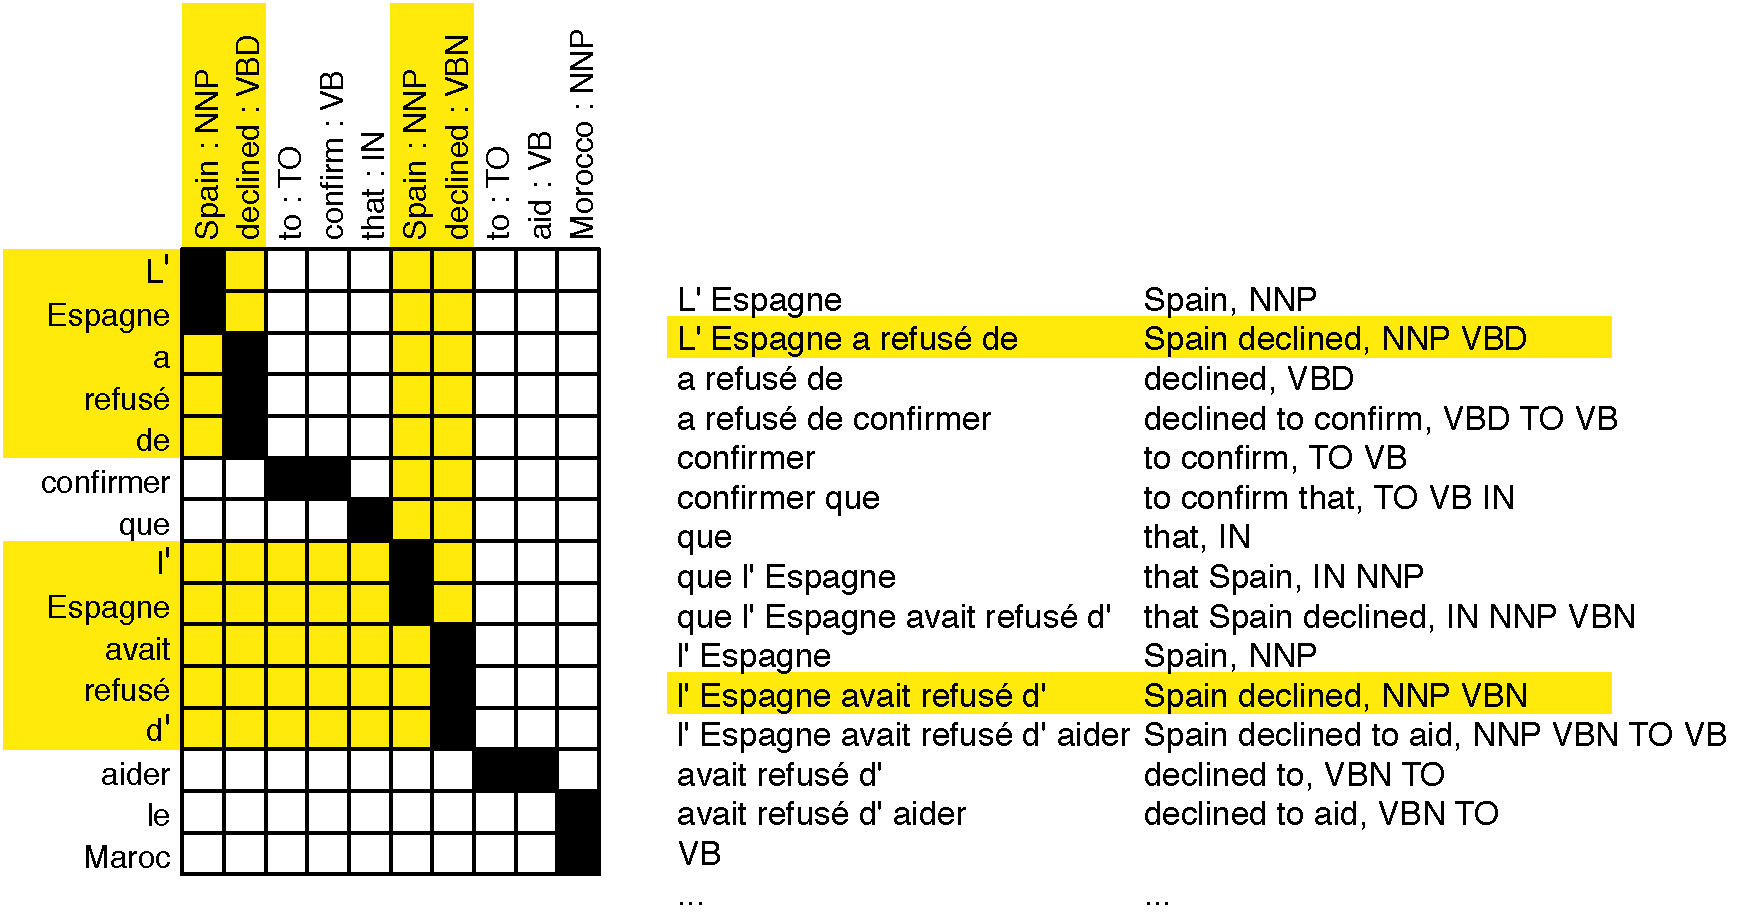
\includegraphics[scale=.55]{images/phrase-extraction-plus-factors}
\end{center}
\caption{Different factors can be combined.  This has the effect of giving different conditioning variables.}\label{phrase-extraction-of-words-and-post-tags}
\end{figure}



If the only occurrences of {\it Spain declined} occurred in the sentence pair given in Figure \ref{word-aligned-parallel-corpus}, the phrase translation probability for the two French phrases under current phrase-based models would be
%
\begin{eqnarray*}
p(\textnormal{{\it l' Espagne a refus\'{e} de}} | \textnormal{{\it Spain declined}}) &=& 0.5 \\
p(\textnormal{{\it l' Espagne avait refus\'{e} d'}} | \textnormal{{\it Spain declined}}) &=& 0.5 
\end{eqnarray*}
%
Under these circumstances the two forms of {\it avoir} would be equiprobable and the model would have no mechanism for choosing between them.  
%
In Factored Translation Models translation probabilities can be conditioned on more information than just words.  For instance, using the combination of factors given in Figure \ref{phrase-extraction-of-words-and-post-tags} we can calculate translation probabilities that are conditioned on both words and parts of speech
\begin{equation}
p(\bar{f}_{words} | \bar{e}_{words}, \bar{e}_{pos})  = \frac{count(\bar{f}_{words},  \bar{e}_{words}, \bar{e}_{pos})}{count( \bar{e}_{words}, \bar{e}_{pos})}\label{multiple-conditioning-factors}
\end{equation}
Whereas in the conventional phrase-based models the two French translations of {\it Spain declined} were equiprobable, we now have a way of distinguishing between them.  We can now correctly choose which form of {\it avoir} to use if we know that the English verb {\it decline} is past tense (VBD) or that it is a past participle (VBN):
%
\begin{eqnarray*}
p(\textnormal{{\it l' Espagne a refus\'{e} de}} | \textnormal{{\it Spain declined, NNP VBN}}) &=& 0 \\
p(\textnormal{{\it l' Espagne avait refus\'{e} d'}} | \textnormal{{\it Spain declined, NNP VBN}}) &=& 1 \\ 
	    & & \\
p(\textnormal{{\it l' Espagne a refus\'{e} de}} | \textnormal{{\it Spain declined, NNP VBD}}) &=& 1 \\
p(\textnormal{{\it l' Espagne avait refus\'{e} d'}} | \textnormal{{\it Spain declined, NNP VBD}}) &=& 0
\end{eqnarray*}


%%%%%%%%%%%%%%%%%%%%%%%%%%%%%
%%%%%%%%%%%%%%%%%%%%%%%%%%%%%

\subsection{New modeling possibilities}\label{better-modeling}

The introduction of factors also allows us to model things we were unable to model in the standard phrase-based approaches to translation.  For instance, we can now incorporate a translation model probability which operates over sequences of parts of speech, $p(\bar{f}_{pos} | \bar{e}_{pos})$.  We can estimate these probabilities straightforwardly using techniques similar to the ones used for phrase extraction in current approaches to statistical machine translation.  In addition to enumerating phrase-to-phrase correspondences using word alignments, we can also enumerate POS-to-POS correspondences, as illustrated in Figure \ref{phrase-extraction-of-pos-tags}.  After enumerating all POS-to-POS correspondences for every sentence pair in the corpus, we can calculate $p(\bar{f}_{pos} | \bar{e}_{pos})$ using maximum likelihood estimation
%
\begin{equation}
p(\bar{f}_{pos} | \bar{e}_{pos})  = \frac{count(\bar{f}_{pos}, \bar{e}_{pos})}{count(\bar{e}_{pos})} 
\end{equation}
%
This allows us to capture linguistic facts within our probabilistic framework.  For instance, the adjective-noun alternation that occurs between French and English would be captured because the model would assign probabilities such that
%
\[ p(\textnormal{NN ADJ} | \textnormal{JJ NN}) > p(\textnormal{ADJ NN} | \textnormal{JJ NN}) \]
%
Thus a simple linguistic generalization that current approaches cannot learn can be straightforwardly encoded in Factored Translation Models.

\begin{figure}
\begin{center}
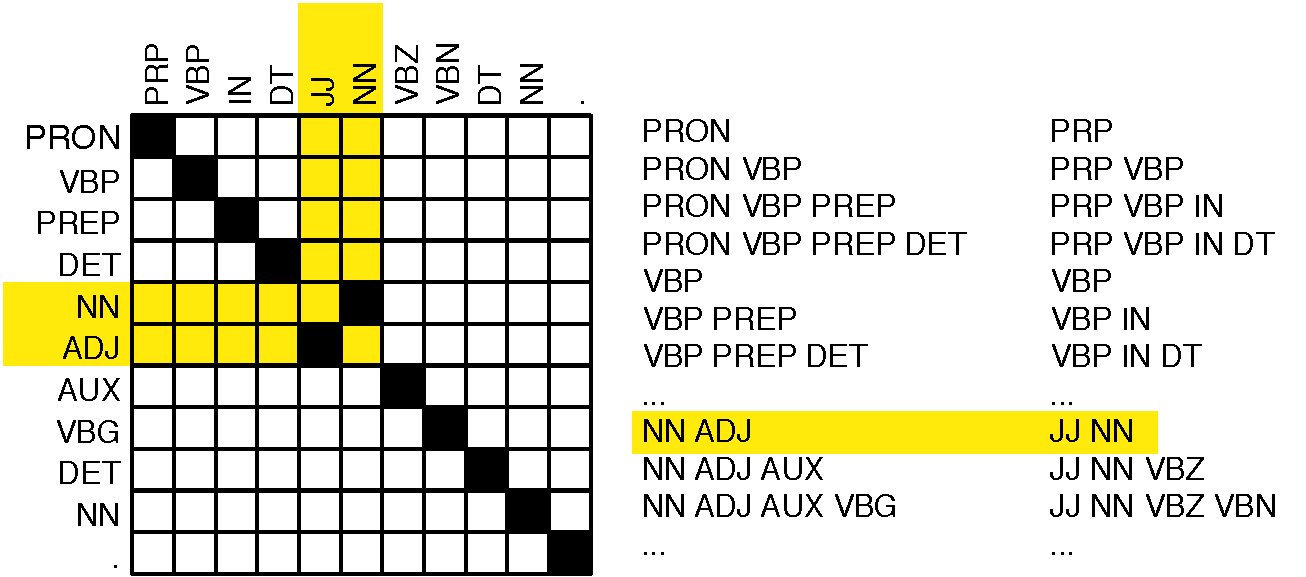
\includegraphics[scale=.55]{images/phrase-extraction-pos-tags-2}
\end{center}
\caption{In factored models correspondences between part of speech tag sequences are enumerated in a similar fashion to phrase-to-phrase correspondences in standard models.}\label{phrase-extraction-of-pos-tags}
\end{figure}

Moreover, part of speech tag sequences are not only useful for calculating translation probabilities such as $p(\bar{f}_{pos} | \bar{e}_{pos})$.  They may also be used for calculating ``language model'' probabilities such as $p(\bar{f}_{pos})$.  The probability $p(\bar{f}_{pos})$ can be calculated similarly to the $n$-gram language model probability $p(\bar{f}_{words})$, which is used in current statistical machine translation systems.   Sequences of parts of speech have much richer counts than sequences of words since the number of unique part of speech tags is much smaller than the number of unique words.  This allows higher order $n$-gram models to be estimated from data.  Practical constraints generally limit us to tri-gram language models over words, but we can accurately estimate 6- or 7-gram language models over parts of speech.




\section{Statistical Modeling}
Factored translation models closely follow the statistical modeling methods used in phrase-based models. Each of the mapping steps is modeled by a feature function. This function is learned from the training data, resulting in translation tables and generation tables.

Phrase-based statistical translation models are acquired from word-aligned parallel corpora by extracting all phrase-pairs that are consistent with the word alignment. Given the set of extracted phrase pairs with counts, various scoring functions are estimated, such as conditional phrase translation probabilities based on relative frequency estimation.

Factored models are also acquired from word-aligned parallel corpora. The tables for translation steps are extracted in the same way as phrase translation tables. The tables for generation steps are estimated on the target side only (the word alignment plays no role here, and additional monolingual data may be used). Multiple scoring functions may be used for generation and translation steps, in our experiments we used
\begin{itemize}
\item five scores for translation steps: conditional phrase translation probabilities in both direction (foreign to English and vice versa), lexical translation probabilities (foreign to English and vice versa), and phrase count;
\item two scores for generation steps: conditional generation probabilities in both directions (new target factors given existing target factors and vice versa).
\end{itemize}

The different components of the model are combined in the log-linear model. In addition to traditional components --- language model, reordering model, word and phrase count, etc. --- each mapping step forms a component with five (translation) or two (generation) features. The feature weights in the log-linear model are determined using a minimum error rate training method \citep{Och2003c}.

\section{Efficient Decoding}
Compared to phrase-based models, the decomposition of the phrase translation into several mapping steps creates additional computational complexity. Instead of a simple table lookup to obtain the possible translation for an input phrase, now a sequence of such tables have to be consulted and their content combined.

Since all translation steps operate on the same segmentation, the {\bf expansion} of these mapping steps can be efficiently pre-computed prior to the heuristic beam search, and stored as translation options (recall the example in Section~\ref{sec:factored-decomposition}, where we carried out the expansion for one input phrase). This means that the fundamental search algorithm does not change. Only the scoring of hypothesis becomes slightly more complex.

However, we need to be careful about the combinatorial explosion of the number of translation options given a sequence of mapping steps. If one or many mapping steps result in a vast increase of (intermediate) expansions, this may be become unmanageable. We currently address this problem by early pruning of expansions, and limiting the number of translation options per input phrase to a maximum number, by default 50.

\section{Current Shortcomings}

One significant limiting factor in the performance of multi-factored
translation models is the due to the present requirement that
successive translation steps all translate identical source and
target spans.  If a compatible translation is not found for a
secondary translation step (either because hypotheses with
compatible factors were discarded earlier or because there is no
possible translation in the phrase table for the secondary
translation step), the hypothesis is abandoned. This has
considerable benefit from a computational perspective since it
constrains the search space for potential targets when translating
secondary factors.  However, it causes a number of significant
problems:
\begin{enumerate}
  \item In models where a secondary factor is both generated from another
target factor and translated from a source factor, any pruning
before both steps have completed runs the risk of producing not just
degraded output, but failing to find any adequate translation.
  \item Because a compatible translation must be found in secondary steps
for a translation hypothesis to survive, it is difficult to filter
secondary translation tables.  This results in very large tables
which are inefficient to load and have considerable memory overhead.
  \item When secondary translation steps fail and hypotheses are
abandoned, the model is forced to rely on shorter translation units
for the primary translation step. This is in direct conflict to the
potential benefits that can be gained by richer statistics.
\end{enumerate}

There are several possible ways that the exact-span match
requirement might be addressed. One solution that is computationally
tractable is to back off to shorter spans only in the event of a
failure to find any possible translation candidates during
subsequent translation steps.  The problem that arises is how the
spans established should be translated once multiple translation
units can be used.  Reordering within phrases is certainly quite
common.  These can be further constrained to either match alignments
that are suggested by the initial span.


\chapter[Experiments with Factored Translation Models]{Experiments with \\ Factored Translation Models}\label{chap:factored-experiments}

This chapter reviews the factored translation model experiments conducted at the summer workshop.  After developing the Moses software during  the workshop, we used it to create different configurations of factored translation models to address particular problematic cases when translating into different languages.  The structure of this chapter is as follows:
\begin{itemize}
\item Section \ref{english-german-experiments} presents our experiments for translation from English into German.  We configured factored models to address German morphology through lemmas, and to integrate part of speech and agreement information to improve grammatical coherence. 
\item Section \ref{english-spanish-experiments} describes factored models for translation from English into Spanish, where Spanish subject-verb and adjective-noun-determiner agreement is explicitly modeled.  These experiments further examine how factored models can be used to improve translation quality in small data scenarios. 
\item Section \ref{english-czech-experiments} compares the performance of three different English to Czech translation models with include lemma and morphological information as factors, and shows that these models result in better translation quality than the baseline phrase-based model. 
\end{itemize}

\section{English-German}\label{english-german-experiments}

German is an example for a language with a relatively rich morphology. Historically, most research in statistical machine translation has been carried out on language pairs with the target language English.

This leads to the question: Does rich morphology pose problems that have not been addressed so far, if it occurs on the target side? Previous research has shown, that stemming morphologically rich input languages leads to better performance. However, this trick does not work when we have to {\it generate} rich morphology.

\subsection{Impact of morphological complexity}
To assess the impact of rich morphology, we carried out a study to see what performance gains could be achieved, if we could generate German morphology perfectlty.

For this, we used a translation model trained on 700,000 sentences of the English--German Europarl corpus (a training corpus we will work throughout this section), and the test sets taken from the 2006 ACL Workshop of Statistical Machine Translation. We trained a system with the standard settings of the Moses system (described in \ref{toolkit}).

English--German is a difficult language pair, which is also reflected in the BLEU scores for this task. For our setup, we achieved a score of 17.80 on the 2006 test set, whereas for other language pairs scores of over 30 BLEU can be achieved. How much of this is due to the morphological complexity of German? If we measure BLEU not on words (as it typically done), but on stems, we can get some idea how to answer this question. As shown in Table~\ref{tab:german:stem-bleu} the stem-BLEU score is 21.47, almost 4 points higher.

\begin{table}
\begin{center}
\begin{tabular}{|c|c|c|} \hline
\bf Method &  \bf devtest & \bf test\\ \hline
BLEU measured on words & 17.76 & 17.80 \\ \hline
BLEU measured on stems & 21.70 & 21.47 \\ \hline
\end{tabular}
\end{center}
\caption{Assessment of what could be gained with perfect morphology: BLEU scores measured on the word leveled on on stemmed system output and reference sets. The BLEU score decreases by 4 points due to errors in the morphology.}
\label{tab:german:stem-bleu}
\end{table}

One of the motivations for the introduction of factored translation models is the problem of rich morphology. Morphology increases the vocabulary size and leads to sparse data problems. We expect that backing off to word representations with richer statistics such as stems or word classes will allow us to deal with this problem. Also, morphology carries information about grammatical information such as case, gender, and number, and by explicitly expressing this information in form of factors will allow us to develop models that take grammatical constraints into account.

\subsection{Addressing data sparesness with lemmas}
The German language model may not be as effectives in machine translation as language models are for English, since its rich morphology fragments the data. This raises the question whether this problem of data sparseness may be overcome by building a language model on lemmas instead of the surface form of words.

\begin{figure}
\begin{center}
\begin{tabular}{cc}
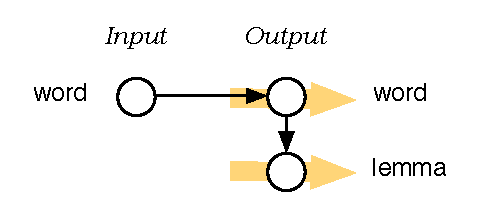
\includegraphics[scale=1]{factored-lemma2.pdf}
&
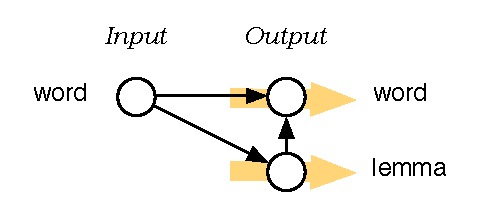
\includegraphics[scale=1]{factored-lemma1.pdf}
\\
Lemma Model 1 & Lemma Model 2
\end{tabular}
\end{center}
\caption{Two models for including lemmas in factored translation models: Both models map words from input to output in a translation step and generate the lemma on the output side. Model 2 includes an additional step that maps input words to output lemmas.}
\label{fig:german:lemma-model}
\end{figure}

To test this hypothesis, we build two factored translation models, as illustrated in Figure~\ref{fig:german:lemma-model}. The models are based on traditional phrase-based statistical machine translation systems, but add additional information in form of lemmas on the output side which allows the integration of a language model trained on lemmas. Note that this goes beyond previous work in reranking, since the second language model trained on lemmas is integrated into the search.

In our experiments, we obtained higher translation performance when using the factored translation models that integrate a lemma language models (all language models are trigram models trained with the SRILM toolkit). See Table~\ref{tab:german:lemma-model} for details. On the two different set sets we used, we gained 0.60 and 0.65 BLEU with Model 1 and 0.19 BLEU and 0.48 BLEU with Model 2 for the two test sets, respectively. The additional translation step does not seem to be useful.

\begin{table}
\begin{center}
\begin{tabular}{|c|c|c|} \hline
\bf Method &  \bf devtest & \bf test\\ \hline
baseline & 18.22 & 18.04 \\ \hline
hidden lemma (gen only) & \bf 18.82 & \bf 18.69 \\ \hline
hidden lemma (gen and trans) & 18.41 & 18.52 \\ \hline
best published results & - & 18.15 \\ \hline
\end{tabular}
\end{center}
\caption{Results with the factored translation models integrating lemmas from Figure~\ref{fig:german:lemma-model}: language models over lemmas lead to better performance, beating the best published results. Note: the baseline presented here is higher than the one used in Table~\ref{tab:german:stem-bleu}, since we used a more mature version of our translation system.}
\label{tab:german:lemma-model}
\end{table}

\subsection{Overall grammatical coherence}
The previous experiment tried to take advantage of models trained with richer statistics over more general representation of words by focussing the the lexical level. Another aspect of words is their grammatical role in the sentence. A straightforward aspect to focus on are part-of-speech tags. The hope is that constraints on part-of-speech tags might ensure more grammatical output.

\begin{figure}
\begin{center}
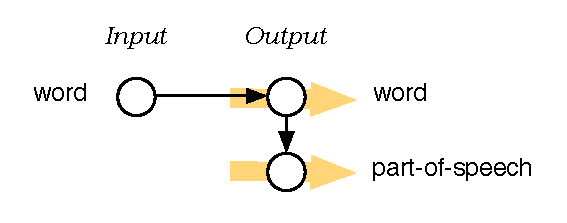
\includegraphics[scale=1]{factored-simple-pos-lm.pdf}
\end{center}
\caption{Adding part-of-speech information to a statistical machine translation model: By generating POS tags on the target side, it is possible to use high-order language models over these tags that help ensure more grammatical output. In our experiment, we only obtained a minor gain (BLEU 18.25 vs. 18.22).}
\label{fig:german:pos-model}
\end{figure}

The factored translation model that integrates part-of-speech information is very similar to the lemma models from the previous section. See Figure~\ref{fig:german:pos-model} for an illustration. Again the additional information on the target side is generated by a generation step, and a language model over this factor is employed.

Since there are only very few part-of-speech tags compared to surface forms of words, it is possible to build very high-order language models for them. In our experiments with used 5-gram and 7-gram models. However, the gains with obtained by adding such a model were only minor: for instance, on the devtest set we imrpoved BLEU to 18.25 from 18.22, while on the test set, no difference in BLEU could be measured.

A closer look at the output of the systems suggests that local grammatical coherence is already fairly good, so that the POS sequence models are not necessary. On the other hand, for large-scale grammatical concerns, the added sequence models are not strong enough to support major restructuring.

\subsection{Local agreement (esp. within noun phrases)}
The expectation with adding POS tags is to have a handle on relatively local grammatical coherence, i.e. word order, maybe even insertion of the proper function words. Another aspect is morphological coherence. In languages as German not only nouns, but also adjectives and determiners are inflected for count (singular versus plural), case and grammatical gender. When translating from English, there is not sufficient indication from the translation model which inflectional form to chose and the language model is the only means to ensure agreement.

By introducing morphological information as a factor to our model, we expect to be able to detect word sequences with agreement violation.  Thus our model should be able to decide that
\begin{itemize}
\item {\bold DET-sgl NOUN-sgl} is a good sequence, but
\item {\bold DET-sgl NOUN-plural} is a bad sequence
\end{itemize}

The model for integrating morphological factors is similar to the previous models, see Figure\ref{fig:german:morphology} for an illustration. We generate a morphological tag in addition to the word and part-of-speech tag. This allows us to use a language model over the tags. Tags are generated with the LoPar parser.

\begin{figure}
\begin{center}
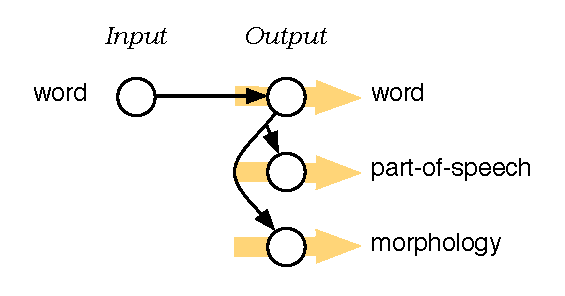
\includegraphics[scale=1]{factored-posmorph-lm.pdf}
\end{center} 
\caption{Adding morphological information: This enables the incorporation of language models over morphological factors and ensure agreement, especially in local contexts such as noun phrases.}
\label{fig:german:morphology}
\end{figure}

When using a 7-gram POS model in addition to the language model, we see minor improvements in BLEU (+0.03 and +0.18 for the devtest and test set, respectively). But an analysis on agreement within noun phrases shows that we dramatically reduced the agreement error rate from 15\% to 4\%. See Table~\ref{tab:german:morphology} for the summary of the results.

\begin{table}
\begin{center}
\begin{tabular}{|c|c|c|c|} \hline
\bf Method & \bf Agreement errors in NP & \bf devtest & \bf test\\ \hline
baseline & 15\% in NP $\ge$ 3 words & 18.22 BLEU & 18.04 BLEU \\ \hline
factored model & 4\% in NP $\ge$ 3 words & 18.25 BLEU & 18.22 BLEU \\ \hline
\end{tabular}
\end{center}
\caption{Results with the factored translation model integrating morphology from Figure~\ref{fig:german:morphology}. Besides minor improvement in BLEU, we drastically reduced the number of agreement errors within noun phrases.}
\label{tab:german:morphology}
\end{table}

Here two examples, where the factored model outperformed the phrase-based baselines:
\begin{itemize}
\item Example 1: rare adjective in-between preposition and noun
\begin{itemize}
\item baseline: {\bold ... \underline{zur} zwischenstaatlichen methoden ...}
\item factored model: {\bold ... zu zwischenstaatlichen methoden ... }
\end{itemize}
\item Example 2: too many words between determiner and noun
\begin{itemize}
\item baseline: {\bold ... \underline{das} zweite wichtige {\"a}nderung ...}
\item factored model: {\bold ... die zweite wichtige {\"a}nderung ... }
\end{itemize}
\end{itemize}

In both cases, the language model over surface forms of words is not strong enough. Locally, on a bigram level the word sequences are correct, due to the ambiguity in the morphology of German adjectives. For instance, {\bold zwischenstaatlichen} could be both singular female dative, as the preposition {\bold zur}, or plural, as the noun {\bold methoden}. The agreement error is between preposition and noun, but the language model has to overcome the context of the unusual adjective {\bold zwischenstaatlichen} which is not very frequent in the training corpus. For the morphological tags, however, we have very rich statistics that rule out the erroneous word sequence.

\subsection{Subject-verb agreement}\label{english-subject-verb-agreement-example}
Besides agreement errors within noun phrases, another source for disfluent German output are agreement errors between subject in verb. In German, subject and verb are often next to each other (for instance, {\bold \underline{hans} \underline{schwimmt}.}), but may also be several words apart, which almost always the case in relative clauses ({\bold ... damit \underline{hans} im see ... \underline{schwimmt}.}).

We could address this problems with factors and skip language models. Consider the following example of a English sentence which may be generated incorrectly by a machine translation system: 

{\bold \begin{center} 
\begin{tabular}{cccccccc}
\bf the & \bf paintings & \bf of & \bf the & \bf old & \bf man & \underline{\bf is} & \bf beautiful \\
\end{tabular}
\end{center}}

In this sentence, {\bold old man is} is a better trigram than {\bold old man are} so the language model will more likely prefer the wrong translation. The subject-verb agreement is between the words {\bold paintings} and {\bold are}, which are several words apart. Since this out of the reach of traditional language models, we would want to introduce tags for subject and verb to check for this agreement. For all the other wirdsm, the tag is empty. See the extended example below:

{\bold \begin{center}
\begin{tabular}{cccccccc}
\bf the & \bf paintings & \bf of & \bf the & \bf old & \bf man & \bf are & \bf beautiful \\
- & SBJ-plural & - & - & - & - & V-plural & - \\
\end{tabular}
\end{center}} 

Given these tags, we should prefer the correct morphological forms:
\begin{center}
{\bold p(-,SBJ-plural,-,-,-,-,V-plural,-) $>$ p(-,SBJ-plural,-,-,-,-,V-singular,-)}
\end{center}

We implemented a skip language model, so that the empty tags are ignored, and the language model decision is simply made on the base of the subject and verb tags:
\begin{center}
{\bold p(SBJ-plural,V-plural) $>$ p(SBJ-plural,V-singular)}
\end{center}

We explored this idea when translating into Spanish, as described in the next section. 

\section{English-Spanish}\label{english-spanish-experiments}


In this section we describe a series of experiments we conducted using
factored models for translation European parliament proceedings from
English to Spanish.  The motivation for these experiments was to
assess the utility of factored translation models for limited resource
translation tasks.  In the standard phrase-based translation paradigm
the translation process is modeled as a $p(\textbf{e}|\textbf{f})$
where the target language sentence $\textbf{e}$ is generated the
source sentence $\textbf{f}$ and both source and target are decomposed
into fully inflected substrings or phrases.  It is because
phrase-based systems directly model the translation strings that they
require large amounts of parallel data to train.  Intuitively, these
data are helpful for modeling both general coocurrence phenomena (such
as local agreement) within a language and phrases that translated
non-compositionally across languages.

In these experiments, we explore the use of factored models to
reduce the data requirements for statistical machine translation.
In these models we attempt to improve on the performance of a standard
phrase-based model either by explicitly address local agreement or by
modeling the translation process through decomposition into different
morphological factors.  Specifically, we explored models that model
lemmatized forms of the parallel training data rather than fully
inflected forms.  We also experimented with models that attempt to
explicitly model agreement through language models of agreement-like
features derived from morphological analysis.

To compare the performance of these models we created a small subset
of Europarl that we call {\tt EuroMini}.  This subset consisted of
40,000 sentence pairs (approximately 5\% of the total Europarl
Corpus).  Table~\ref{tab:euromini-corpus-stats} shows the statistics
for this corpus and BLEU scores from a baseline phrase-based MT system. For
these tasks we report results translating from English into Spanish.
We choose this task to test whether our factored models could better
model the explicit agreement phenomena in Spanish.  We compared the
results of systems trained on this reduced form of Europarl with:
\begin{enumerate}
  \item standard models trained on {\tt EuroMini}
  \item standard models trained with {\tt EuroMini} with Spanish-side of full Europarl.
  \item standard models trained on full Europarl
\end{enumerate}
\begin{table}
  \begin{center}
    \begin{tabular}{|l|c|l|l|}
      \hline
      \bf Data Set & \bf Translation Direction & \bf Size & \bf Baseline (with different LMs) \\ \hline \hline
      Full Europarl & English $\rightarrow$ Spanish  & 950k LM Train       &  3-gram LM $\rightarrow$ 29.35 \\
                                                  &  & 700k Bitext         &  4-gram LM $\rightarrow$ 29.57 \\
                                                  &  &                     &  5-gram LM $\rightarrow$ 29.54 \\ \hline
      \tt EuroMini & English $\rightarrow$ Spanish   & 60k LM Train        &  3-gram LM $\rightarrow$ 23.41 \\
                                                   & & 40k Bitext          &  3-gram LM $\rightarrow$ 25.10 (950k train) \\
      \hline
    \end{tabular}
  \end{center}
  \caption{{\tt EuroMini} and Europarl English-Spanish Corpus Description}
  \label{tab:euromini-corpus-stats}
\end{table}

\subsection{Sparse Data and Statistical MT for English-Spanish}

Like many languages, Spanish exhibits both subject-verb agreement and
noun-phrase internal agreement.  Spanish verbs must agree with their
subjects in both number and person.  Spanish noun phrases force
determiners, adjectives and nouns to agree in both number and gender.
In both cases, the agreement is explicitly marked in Spanish
morphology. Examples of these agreement phenomena are shown in
Table~\ref{tab:spanish-agr-examples}.
\begin{table}
  \begin{center}
    \begin{tabular}{|l|llll|}
      \hline
      \multicolumn{5}{|c|}{\it Subject Verb Agreement} \\ \hline \hline
      \bf Spanish & \bf T\'{u} & \bf quieres & un & billete \\
      \bf Gloss & you [2p, sing] & want [2p, sing] & a & ticket \\ 
      \hline
    \end{tabular}

    \begin{tabular}{|l|lllllllll|}
      \hline
      \multicolumn{10}{|c|}{\it Long Distance Subject Verb Agreement} \\ \hline \hline
      \bf Spanish & La & \bf creaci\'{o}n & de & un & grupo & de & alto & nivel & \bf es \\
      \bf Gloss & The & creation [3p, sing] & of & a & group & of & high & level/standing & is [3p, sing]\\
      \hline
    \end{tabular}

    \begin{tabular}{|l|lll|}
      \hline
      \multicolumn{4}{|c|}{\it Noun Phrase Agreement} \\ \hline \hline
      \bf Spanish & \bf esta & \bf cooperaci\'{o}n & \bf reforzada \\
      \bf Gloss & this [sing, f] & cooperation [sing, f] & reinforced/enhanced [sing, f] \\
      \hline
    \end{tabular}
  \end{center}
  \caption{Examples of Spanish Agreement Phenomena}
  \label{tab:spanish-agr-examples}
\end{table}

The inflectional morphology that marks these phenomena in Spanish
presents a unique set of problems for statistical language learning in
general and MT in specific.  First, methods based on counts of surface
form words suffer from data fragmentation.  Compare, for instance, the
English phrase ``saw the'' (as in ``I/he/she/they [ saw the ]
car/bag'') with it's possible Spanish translation (shown in Table~\ref{tab:example-frag}).

\begin{table}[h]
    \begin{center}
      \begin{tabular}{|l|l||l|l|}
        \hline
        vi al & vi a la & viste al & viste a la \\ \hline
        vio al & vio a la & vimos al & vimos a la \\ \hline
        vieron al & vieron a la & visteis al & visteis a la \\ 
        \hline
      \end{tabular}
    \end{center}
    \caption{Examples of Data Fragmentation Due to Poor Generalization}
    \label{tab:example-frag}
\end{table}

Each surface shown here differs by only person and number features on
the verb ``ver'' or the gender on the determiner ``el.''  Instead of
of learning a relation between underlying lemmatized form ``ver a el''
and the corresponding English phrase, a standard MT system must learn
each of the variants shown above.  In situations where training data is
abundant, this may not cause great difficulty, but when parallel
training resources are lacking, the fragmentation shown here could
cause poor estimation of translation probabilities.  Furthermore, in
these situations observation of each phrase variant may not be
possible, and a statistical model based on surface forms alone would
not be able to produce unseen variants.  For statistical MT systems,
the lack of ability to generalize could affect all stages of training
including word alignment, phrase extraction and language model
training.

A second set of problems in Spanish has to do with long distance
agreement and is similar to the English example given in Section \ref{english-subject-verb-agreement-example}.  In this case, inflectional morphology
enforces an agreement relation between two surface forms across a long
span.  Phrase-based MT systems have difficulty modeling this
agreement: typically neither language models or phrase translation
models can be reliably estimated for dependencies longer than 3-4
words.  This problem is exacerbated in sparse data conditions, and we
hypothesize that in these conditions, long term coherence of
phrase-based MT output could suffer.

In the sections below we detail two factored translation models that
attempt to address these problems specifically.  Both models extend
the standard surface form model by using morphological analysis and
part of speech information.  To address the agreement and long-span
coherence problems, we construct a model that {\it generates}
agreement features and {\it checks} these features using a language
model trained over morphological features.

We extend this model to address the problems of poor generalization by
decomposing the surface-form translation process into two parallel
processes: translation of lemmas and morphological features.  Lemmas
and morphological features are then recombined in a generation process
to create target surface forms. Details of both these models and
experiments we conducted with them are described below.

For both sets of experiments {\tt EuroMini} data was preprocessed to
using FreeLing~\cite{Atserias:2006} for both part of speech tags and
morphological analysis.

\subsection{Explicit Agreement and Coherence Models}

In these experiments, we applied factored models as an extension to
standard phrase-based MT.  In these experiments standard
surface-to-surface translation is performed, but we add stochastic
constraints on possible target hypotheses to limit enforce (in a soft
way) agreement relations.  This is done by generating a latent factor
(in this case morphological features) from each target word that is
hypothesized during decoding.  Hypotheses are then scored with both
standard MT model components and language models trained over
agreement features.  Figure~\ref{fig:latent-factor-check} shows the
configuration of two models described below: Verb/Noun/Preposition
(VNP) and Noun/Determiner/Adjective (NDA).

\begin{figure}[t]
\begin{center}
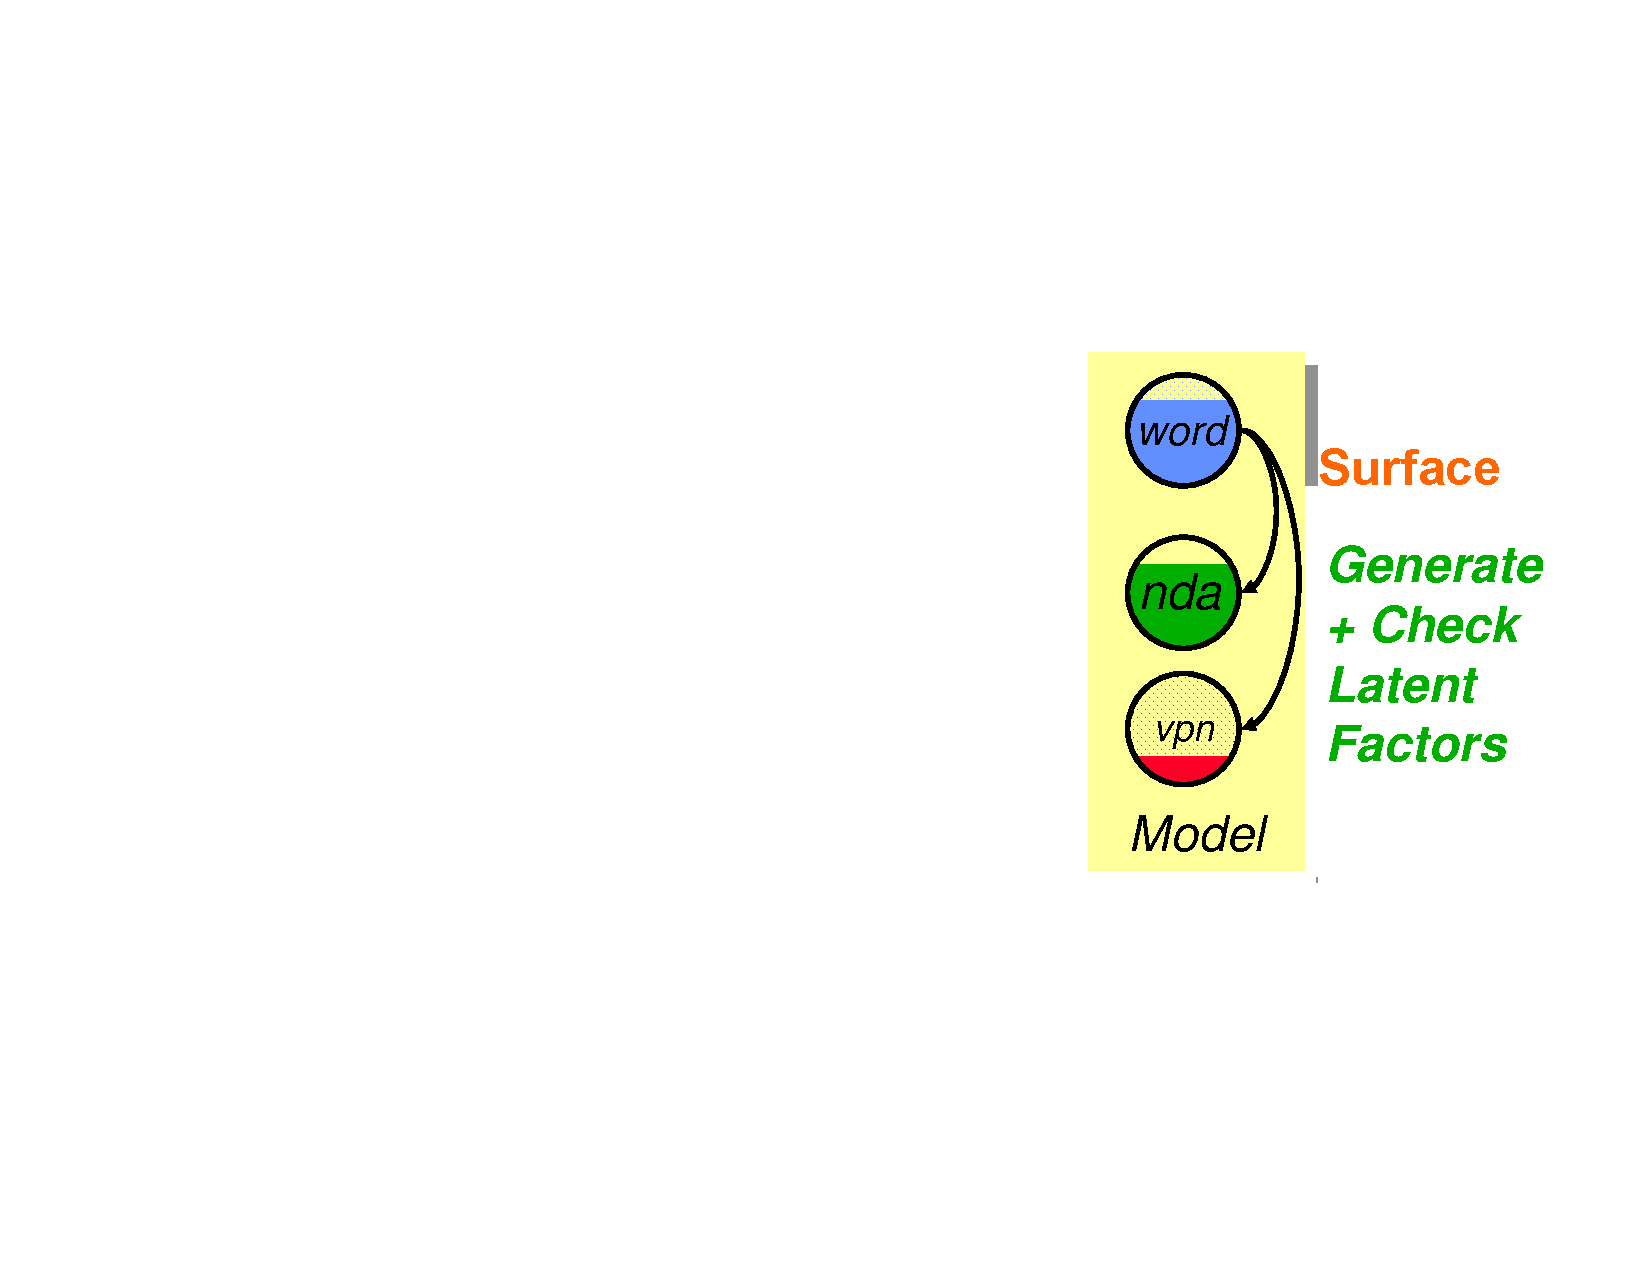
\includegraphics[width=4cm]{wade-latent-factors} 
\caption{Latent Factor Checking using Agreement Features}
\label{fig:latent-factor-check}
\end{center}
\end{figure}

This configuration was also used with POS tags to ensure long term
coherence.  Table~\ref{tab:LM-models} summarizes different models to explicitly
check for agreement and ensure coherence.

\begin{table}[h]
  \begin{center}
    \begin{tabular}{|l|l|}
      \hline
      \bf Problems Addressed & \bf Model Type \\ \hline \hline
      Explicit Agreement & -- LMs over verbs + subjects \\
                         & -- LMs over nouns + determiners + adjectives \\
      \hline
      Long Span Coherence & -- LMs over POS Tags \\
      \hline
    \end{tabular}
  \end{center}
  \caption{LM-based Agreement and Coherence Models}
  \label{tab:LM-models}
\end{table}
\subsubsection{}

\subsubsection{Verb/Subject and Noun-Phrase Agreement Models}

In a first set of experiments we used features derived from a
morphological analysis of the training data to create n-gram language
models.

We produced two models for experimentation.  In one, NDA, number and
gender features were generated for each noun, determiner and adjective
in a hypothesis during decoding.  Non-NDA words deterministically
generated ``don't care'' features.

In a second model, VNP, features required for Spanish verb-subject
agreement were chosen in addition the identity of preposition in
hypothesized sentences.  The inclusion of prepositions allows us
potentially to model the selection relationship between verbs and
prepositions (though this is not strictly an agreement phenomenon).

Table~\ref{tab:nda-vnp} shows the features used for both these models
and their possible values.

\begin{table}[h]
  \begin{center}
    \begin{tabular}{|l|}
      \hline
      \bf NDA Features \\ \hline \hline
      {\bf Gender:} {\it masc, fem, common, none} \\ \hline
      {\bf Number:} {\it sing, plural, invariable, none} \\ \hline \hline
      \bf VNP Features \\ \hline \hline
      {\bf Number:} {\it sing, plural, invariable, none} \\ \hline
      {\bf Person:} {\it 1p, 2p, 3p, none} \\ \hline
      {\bf Prep-ID:} {\it preposition, none} \\ \hline
    \end{tabular}
  \end{center}
  \caption{Latent Features used for NDA and VNP models}
  \label{tab:nda-vnp}
\end{table}

Since ``don't care'' values can intervene between words with NDA and
VNP features, we also experimented with language models that skip
words lacking features of interest.  This effectively increases the
context length for our n-gram based models and should yield more
robust estimation.  This is shown schematically in
Figure~\ref{fig:skipped-lm-nda-vnp}.  Factors marked with ``X'' are not
scored in VNP or NDA language models.

\begin{figure}[t]
\begin{center}
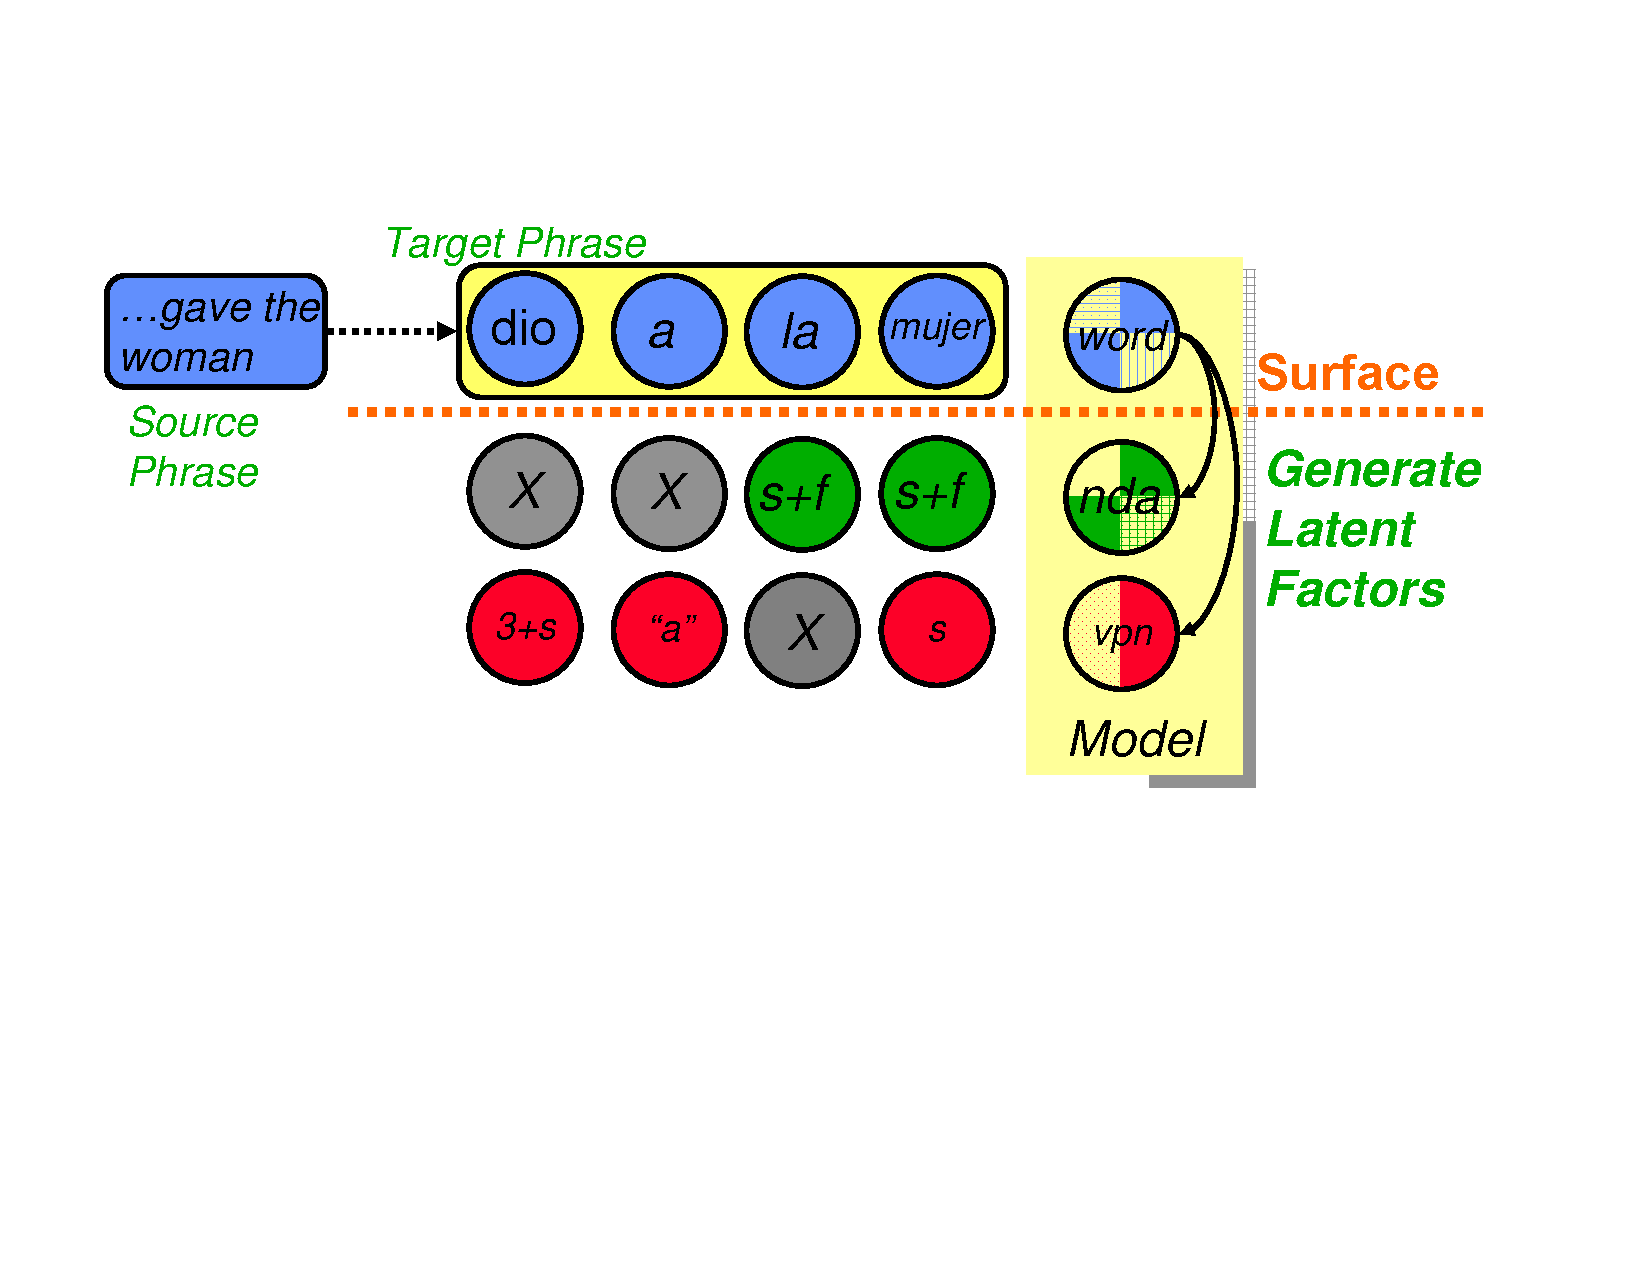
\includegraphics[width=10cm]{wade-skipped} 
\caption{Latent Factor Checking using Agreement Features}
\label{fig:skipped-lm-nda-vnp}
\end{center}
\end{figure}

Results with models {\tt EuroMini} corpus using the standard 60k-word
3-gram language model and evaluated against the 2005 ACL Workshop
Shared Task are shown in Table~\ref{tab:nda-vnp-perf}.  Both NDA and
VPN models improve performance over the baseline system.  We ran
additional experiments that incorporated all morphological features
from our analyzer and this too improved the performance of the system,
though inclusion of part of speech information did not.  The use of
all morphological features closes the gap between the baseline system
and it's large LM counterpart by 74\%, suggesting that better target
language modeling could compensate for the sparsity of target language
data.

\begin{table}[h]
  \begin{center}
    \begin{tabular}{|l|r|}
      \hline
      \bf Model & \bf BLEU \\ \hline \hline
      {\bf Baseline} & 23.41 \\ \hline
      {\bf Baseline + 950k LM} & 25.10 \\ \hline
      {\it NDA} & 24.47 \\ \hline
      {\it VPN} & 24.33 \\ \hline
      {\bf BOTH} & {\bf 24.54} \\ \hline \hline
      {\it NDA w/skipping} & 24.03 \\ \hline
      {\it VPN w/skipping} & 24.16 \\ \hline \hline
      {\bf All Morph Features} & {\bf 24.66} \\ \hline
      {\it All Morph Features + POS Tag} & 24.25 \\ \hline
    \end{tabular}
  \end{center}
  \caption{Latent Features used for NDA and VNP models}
  \label{tab:nda-vnp-perf}
\end{table}

Unfortunately, the use of skipping models didn't improve performance.
Further experiments will be necessary as interactions with pruning
during decoding may have limited the performance of these systems.

\subsubsection{Lemma-based Models for Translation}

The agreement models describe above use a factored approach to add
statistical constraints on target language sequences.  We attempted to
extend this model by improving the underlying translation modeling.
To do this, we created a parallel translation model in which source
words are decomposed into base lemma and morphological features.  Both
lemmas and morphological features are translated from the source to
the target language.  Target words are then re-composed through a
statistically trained generation process on the target side.  This
process is shown schematically in Figure~\ref{fig:parallel-trans}.
Language models are then applied to both morphological features and
surface forms to constrain the output.

\begin{figure}[t]
\begin{center}
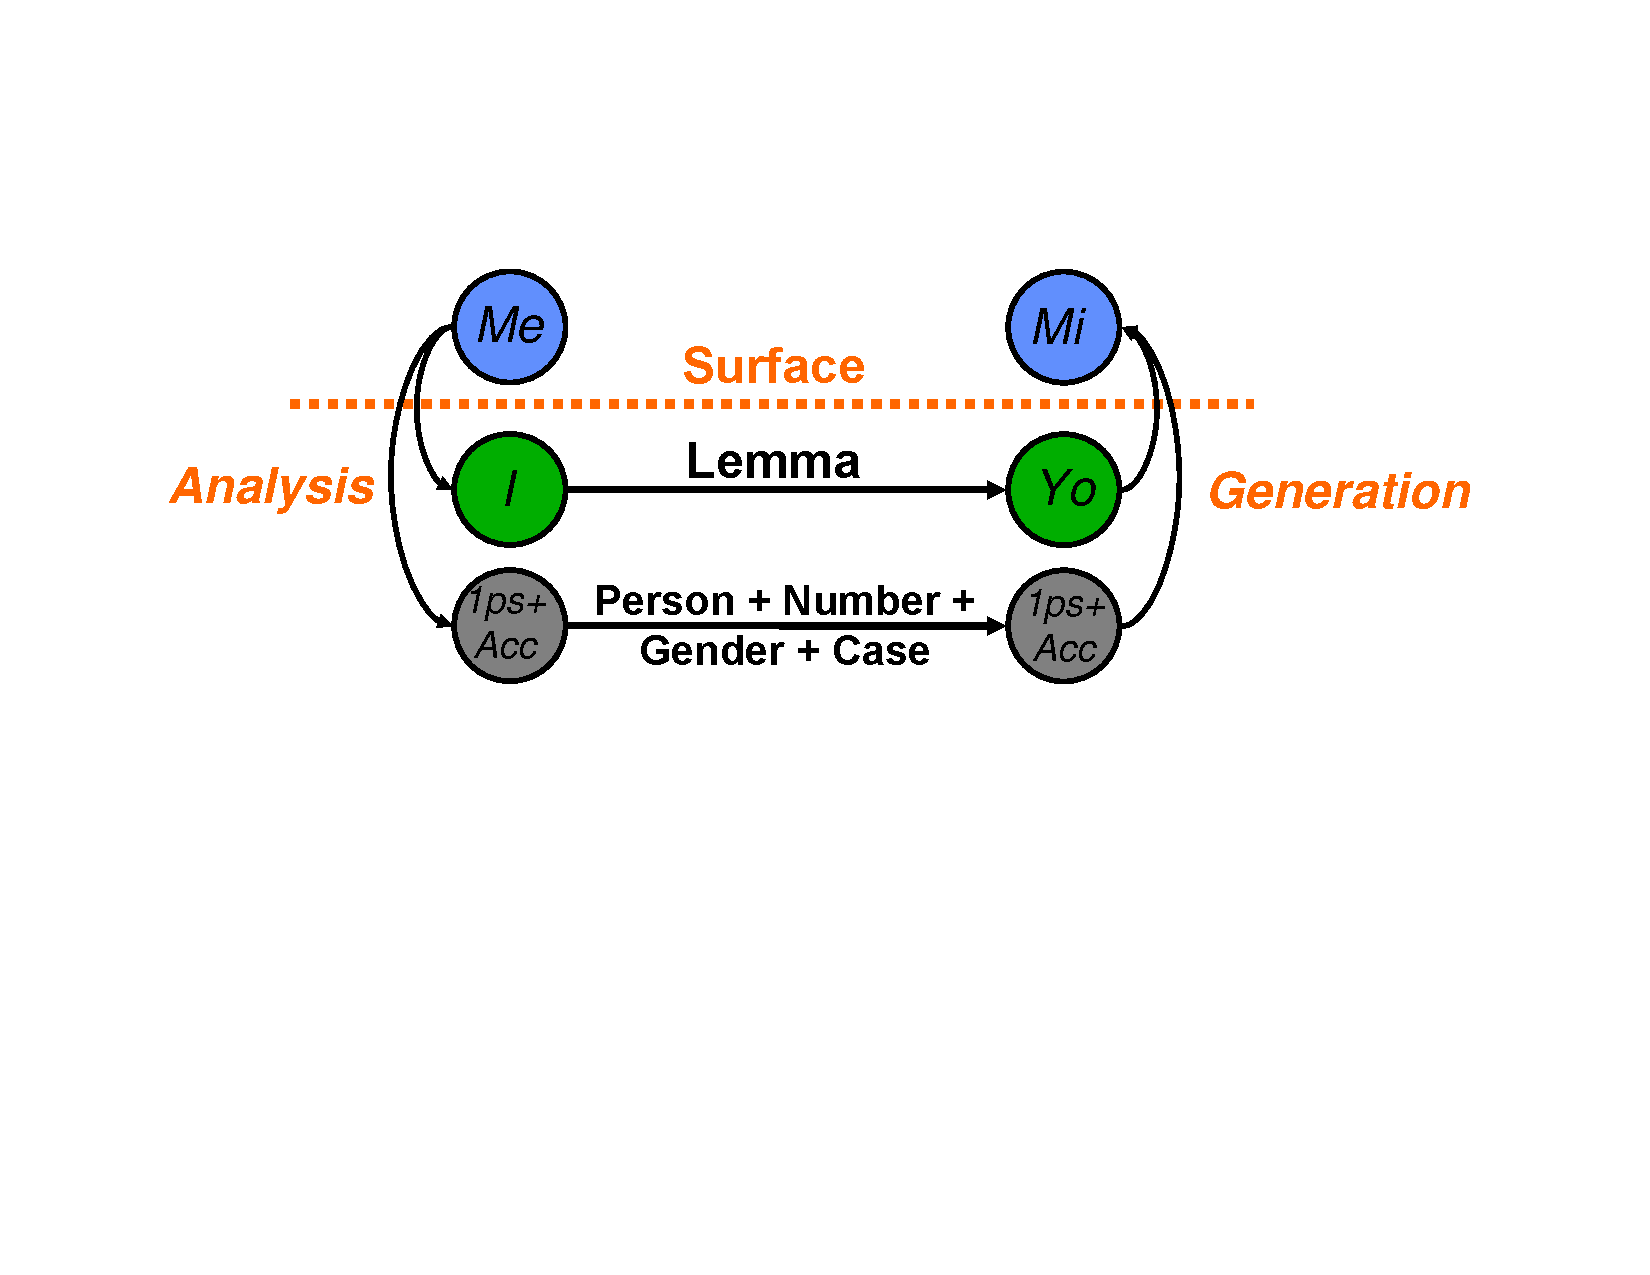
\includegraphics[width=10cm]{wade-parallel-trans} 
\caption{A Factored Model for Parallel Translation of Lemmas and Morphology}
\label{fig:parallel-trans}
\end{center}
\end{figure}

Table~\ref{tab:lemma+morph-results} shows the performance of this
system on a 2005 ACL Workshop Shared Task when a large language model
was used (trained with 950k sentences).  As these
experiments show, the lemma+morphology can lead to improvements through better translation modeling and with the addition of a morphology LM.


\begin{table}[h]
  \begin{center}
    \begin{tabular}{|l|r|}
      \hline
      \bf Model & \bf BLEU \\ \hline \hline
      {\it Baseline} & 25.10 \\ \hline
      {\it Lemma + Morph  } & 25.93 \\ 
      {\it Lemma + Morph plus Morph LM} & 26.11 \\ 
      \hline
    \end{tabular}
  \end{center}
  \caption{Results from Lemma+Morphology Models}
  \label{tab:lemma+morph-results}
\end{table}


\subsubsection{Scaling Up: POS and Morphology models for Large Data Problems}

As long span coherence and agreement remain problems for systems
trained on large data, we attempted apply factored models to improve
of our large-scale, phrase-based models by using high-order n-gram POS
and POS+morphology language models.  As Figure~\ref{fig:POS-lm} shows,
the performance of these models doesn't seem to improve systems
trained on large data.

\begin{figure}[t]
\begin{center}
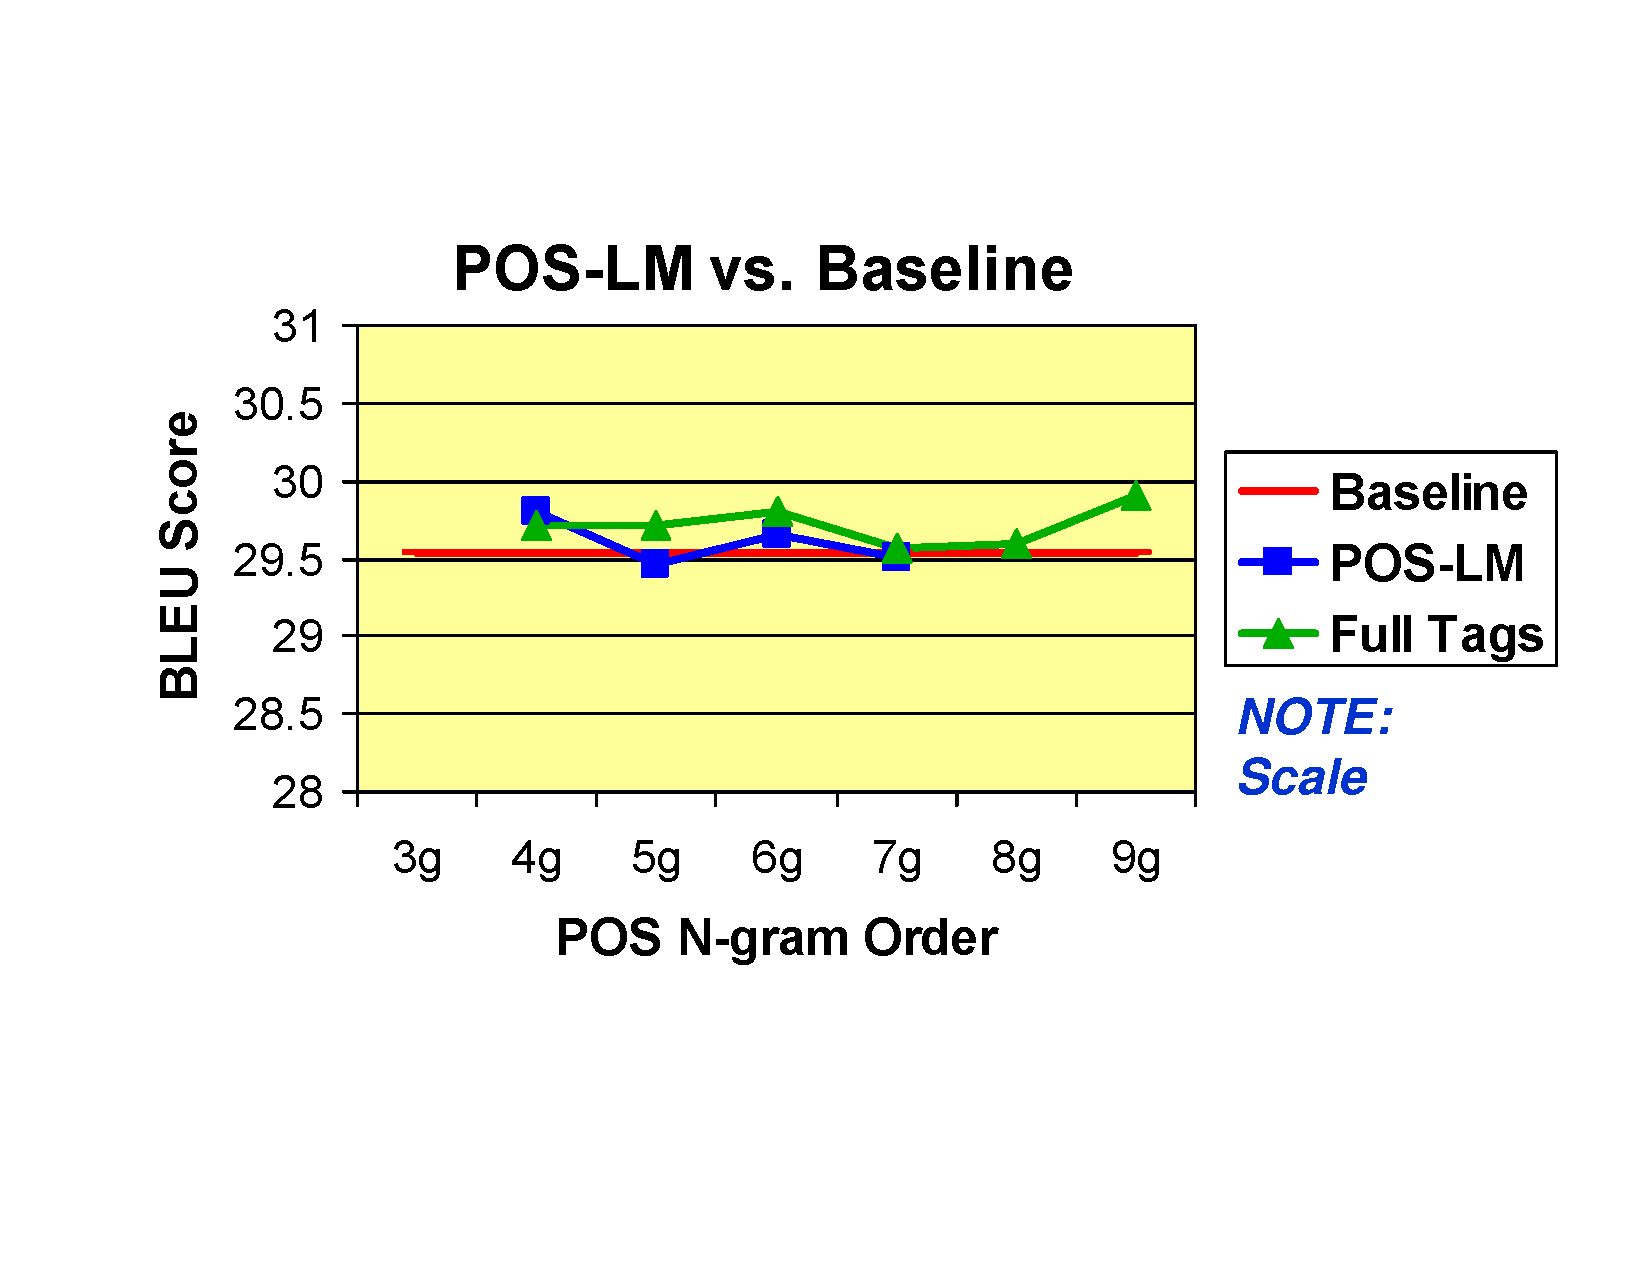
\includegraphics[width=10cm]{wade-pos-lm} 
\caption{Use of Part of Speech Language Models to Improve Long-Span Coherence}
\label{fig:POS-lm}
\end{center}
\end{figure}

Although some small gains may be had using POS tags with morphological
information in this setting, they are much less pronounced (if at all)
than the in the limited {\tt EuroMini} training condition: best-case
improvement with large data (1.2\% relative, 0.4 BLEU absolute)
vs. improvement with {\tt EuroMini} (3.5\% relative, 0.84 BLEU
absolute).  Larger amounts of training data seem to allow the baseline
MT system's language and translation models to better learn Spanish
agreement constraints.  Though not possible during the workshop, in
future experiments we hope to examine the effects of scaling parallel
translation models to large training as well.  



\section{English-Czech}\label{english-czech-experiments}

{
\def\clap#1{\hbox to 0pt{\hss #1\hss}}
\def\equo#1{``#1''}
\def\ang#1{{$\langle${#1}$\rangle$}}  % snadny zapis spicatych zavorek
\def\text#1{{\it{}#1}}


\def\bidir{Czech$\leftrightarrow$English}
\def\tocs{English$\rightarrow$Czech}
\def\toen{Czech$\rightarrow$English}
\def\parcite#1{(\cite{#1})}
\def\perscite#1{\cite{#1}} % works like newcite

\def\max#1{{\bf{} #1}}
\def\stddev#1{{$\pm$#1}}


\subsection{Motivation: Margin for Improving Morphology}
\label{margin-main}

Czech is a Slavonic language with very rich morphology and relatively free word
order. (See e.g. \cite{bojar:cslp:2004} for more details.) The Czech
morphological system defines 4,000 tags in theory and 2,000 were actually seen
in a big tagged corpus. (For comparison, the English Penn Treebank tagset
contains just about 50 tags.) When translating to Czech, any MT system has to
face the richness and generate output words in appropriate forms.

Table \ref{morphmargin-main} displays BLEU scores of single-factored translation
\tocs{} using the baseline corpus only. The second line in the table gives the
scores if morphological information was disregarded in the evaluation: the MT
output is lemmatized (word forms replaced with their respective base forms) and evaluated against lemmatized references.

\begin{table}[ht]
\begin{center}
\begin{tabular}{lccc}
%     &  pcedt .t0-0. t0-0 LM0-3-pcedt  &                &            &  \\
  &  Dev (std)  &  Dev (opt)  &  Test (opt)\\
\hline
Regular BLEU, lowercase  &  25.68  &  29.24  &  25.23\\
Lemmatized MT output\\
\quad{}against lemmatized references  &  34.29  &  38.01  &  33.63\\
%margin:  &  8.61  &  8.77  &  8.40\\
\end{tabular}
\end{center}
\caption{Margin in BLEU for improving morphology.}
\label{morphmargin-main}
\end{table}

We see that more than 8 point BLEU absolute could be achieved if output word
forms were chosen correctly.\footnote{Although not all required word forms may
be available in the training data, we could easily generate output word forms
from lemmas and morphological tags deterministically using a large
target-side-only dictionary.} This observation gives us a strong motivation for
focussing on morphological errors first.



\subsection{Scenarios Used}

We experimented with the following factored translation scenarios:

%\begin{tabular}{c@{\hspace{1cm}}c}
%English  &  Czech\\
%\hline
%\Rnode{elc}{lowercase}  &  \Rnode{clc}{lowercase}\\
%\end{tabular}
%\psset{nodesep=5pt,arrows=->}
%\everypsbox{\scriptstyle}
%\ncLine{elc}{clc}

\begin{figure}
\begin{center}
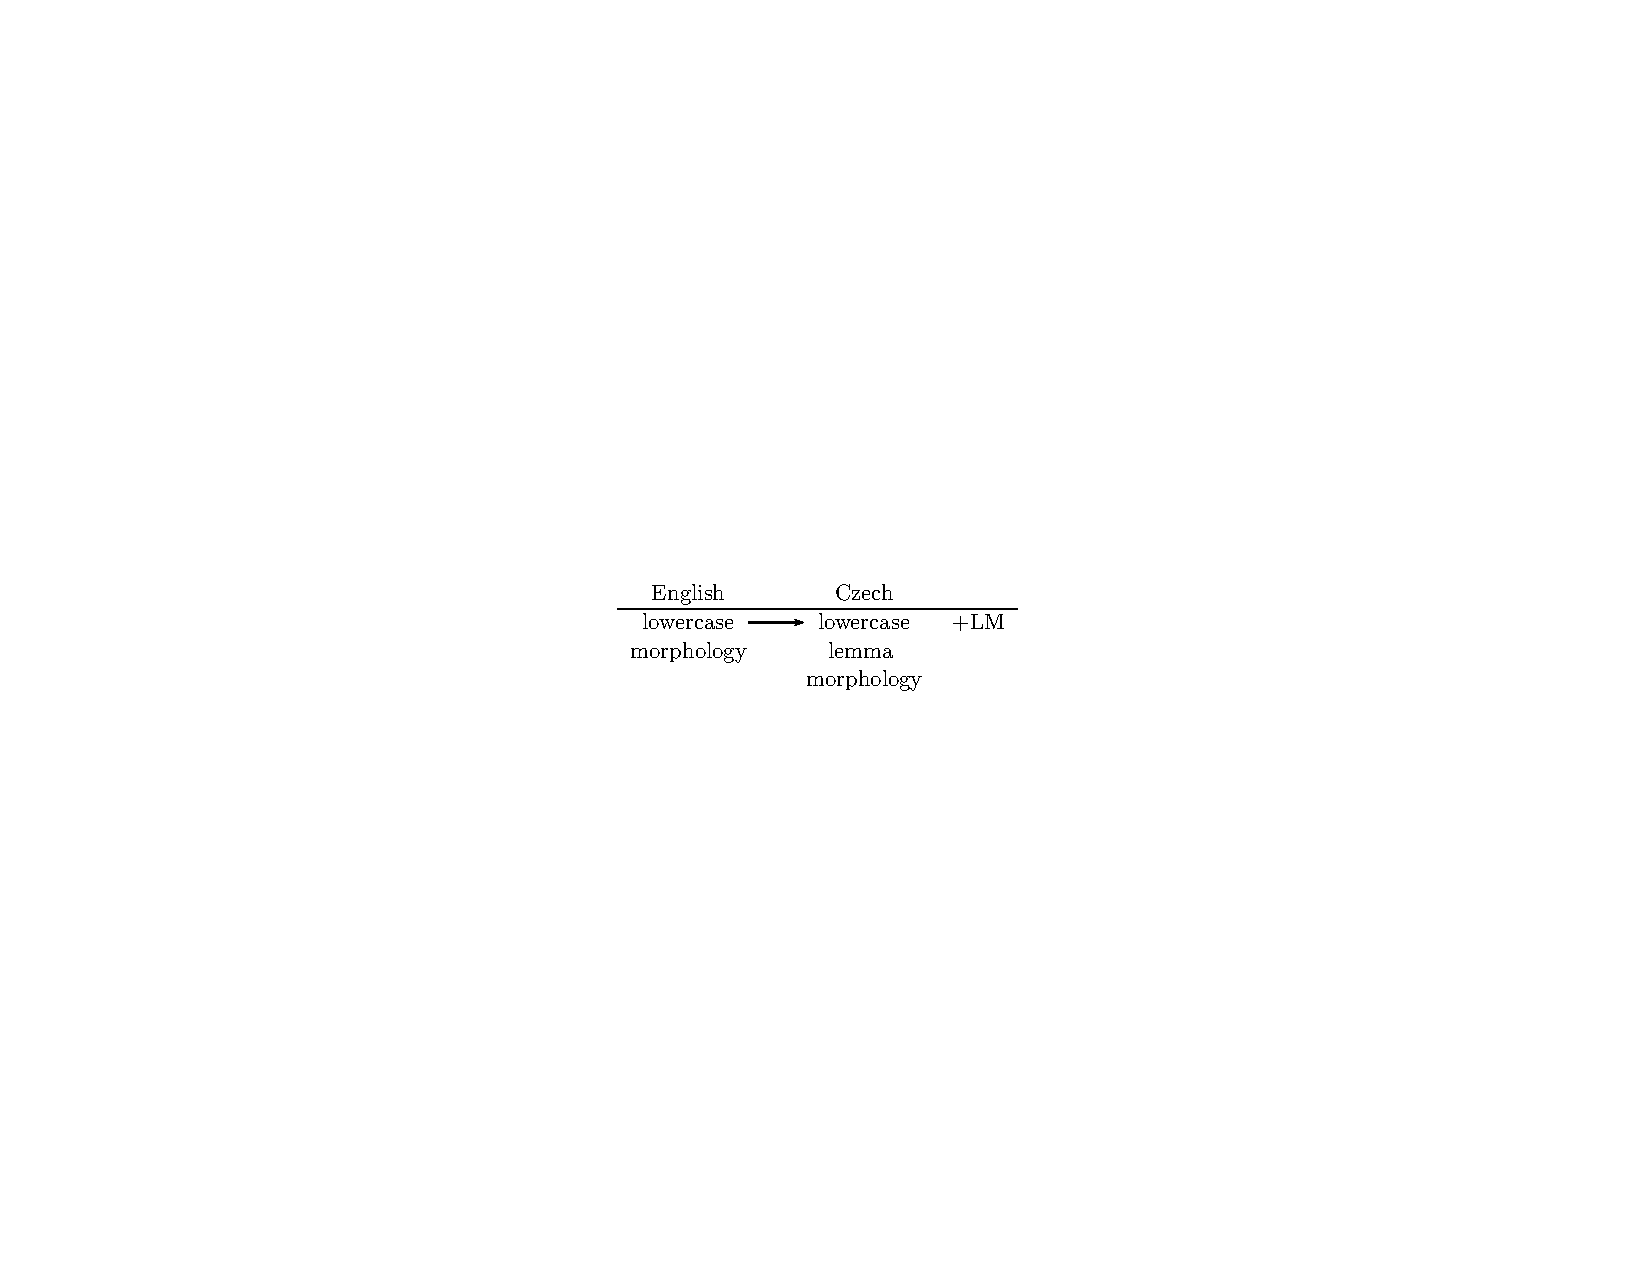
\includegraphics{images/ondrej-picture-1}
\caption{Single-factored scenario (T).}
\end{center}
\end{figure}


The baseline scenario is single-factored: input (English) lowercase word forms
are directly translated to target (Czech) lowercase forms. A 3-gram language
model (or more models based on various corpora) checks the stream of output word forms.

We call this the \equo{T} (translation) scenario.

\begin{figure}
\begin{center}
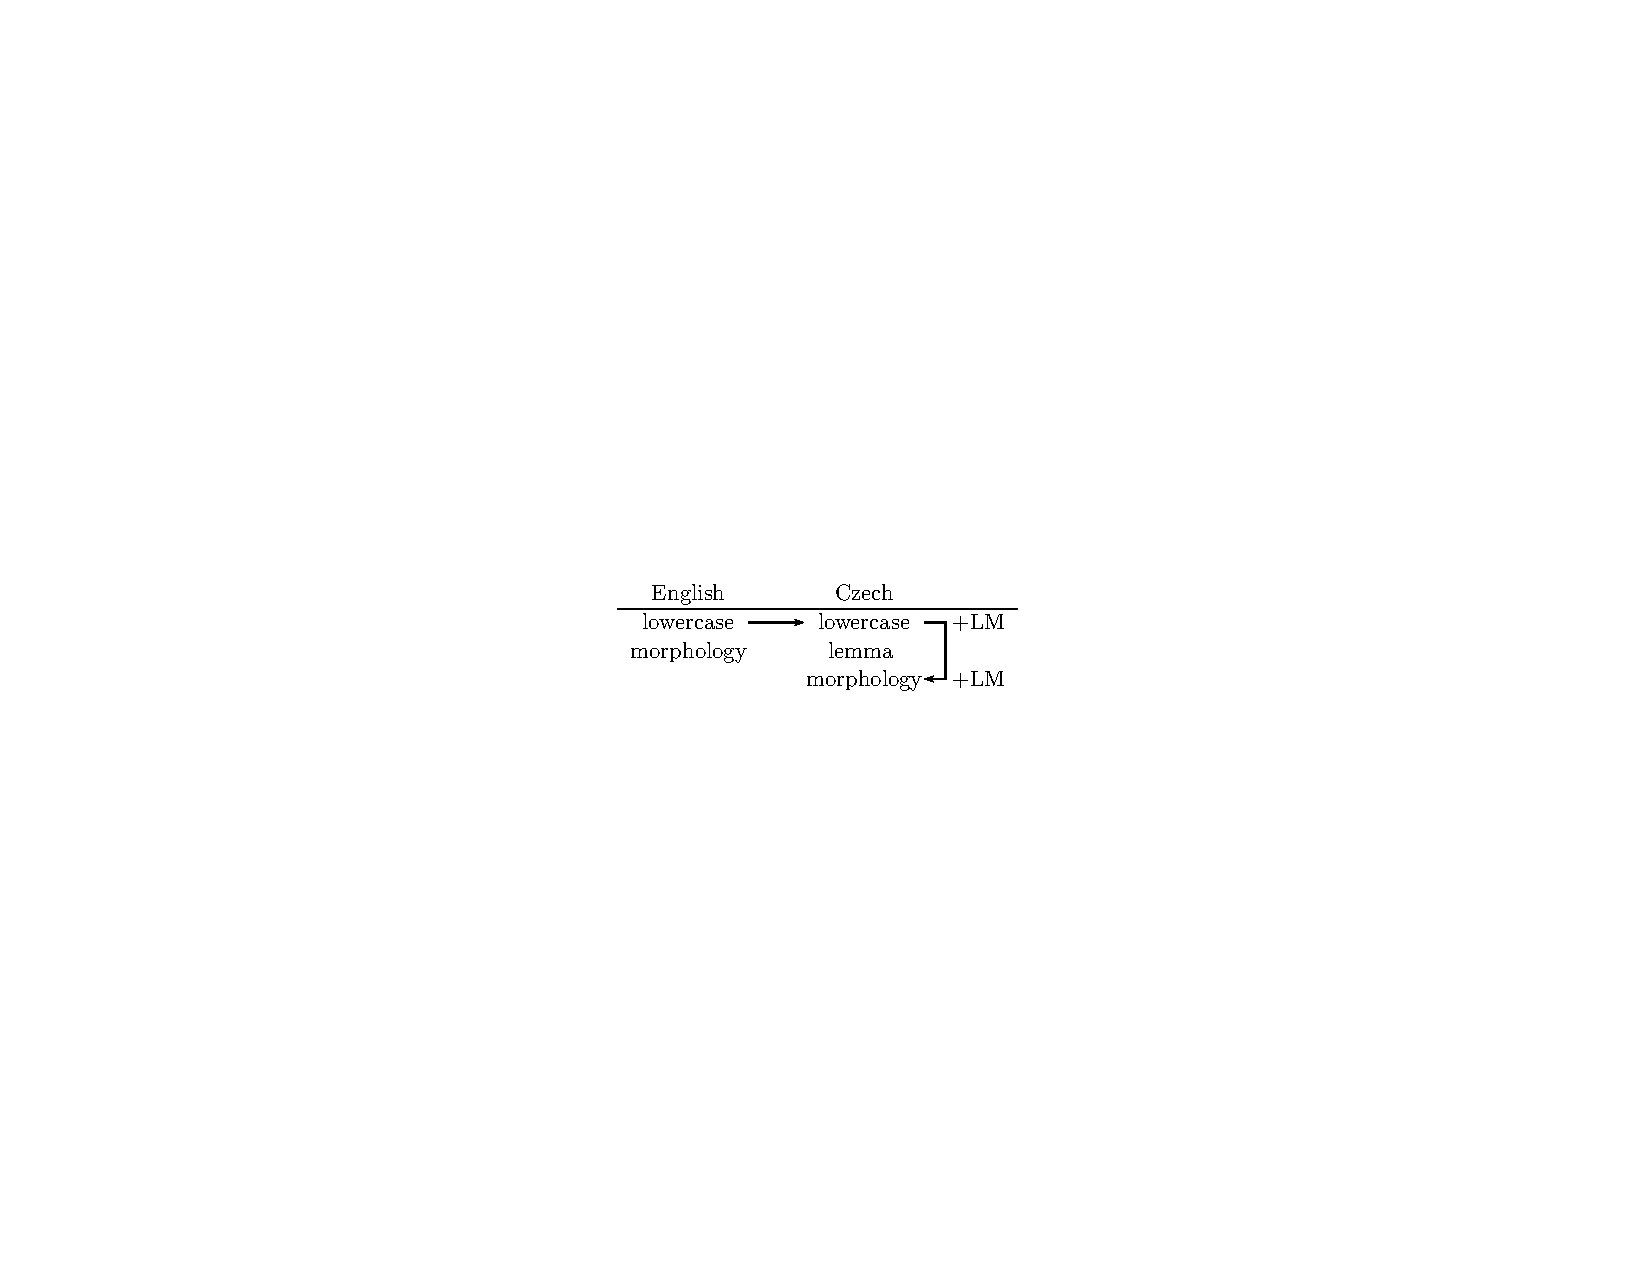
\includegraphics{images/ondrej-picture-2}
\caption{Checking morphology (T+C).}
\end{center}
\end{figure}



In order to check the output not only for word-level coherence but also
for morphological coherence, we add a single generation step: input word forms
are first translated to output word forms and each output word form then
generates its morphological tag.

Two types of language models can be used simultaneously: a (3-gram) LM over word forms and a
LM over morphological tags. For the morphological tags, a higher-order LM can be
used, such as 7 or 9-gram.

We used tags with various levels of detail, see section \ref{posgranularity}.
We call this the \equo{T+C} (translate and check) scenario.



\begin{figure}
\begin{center}
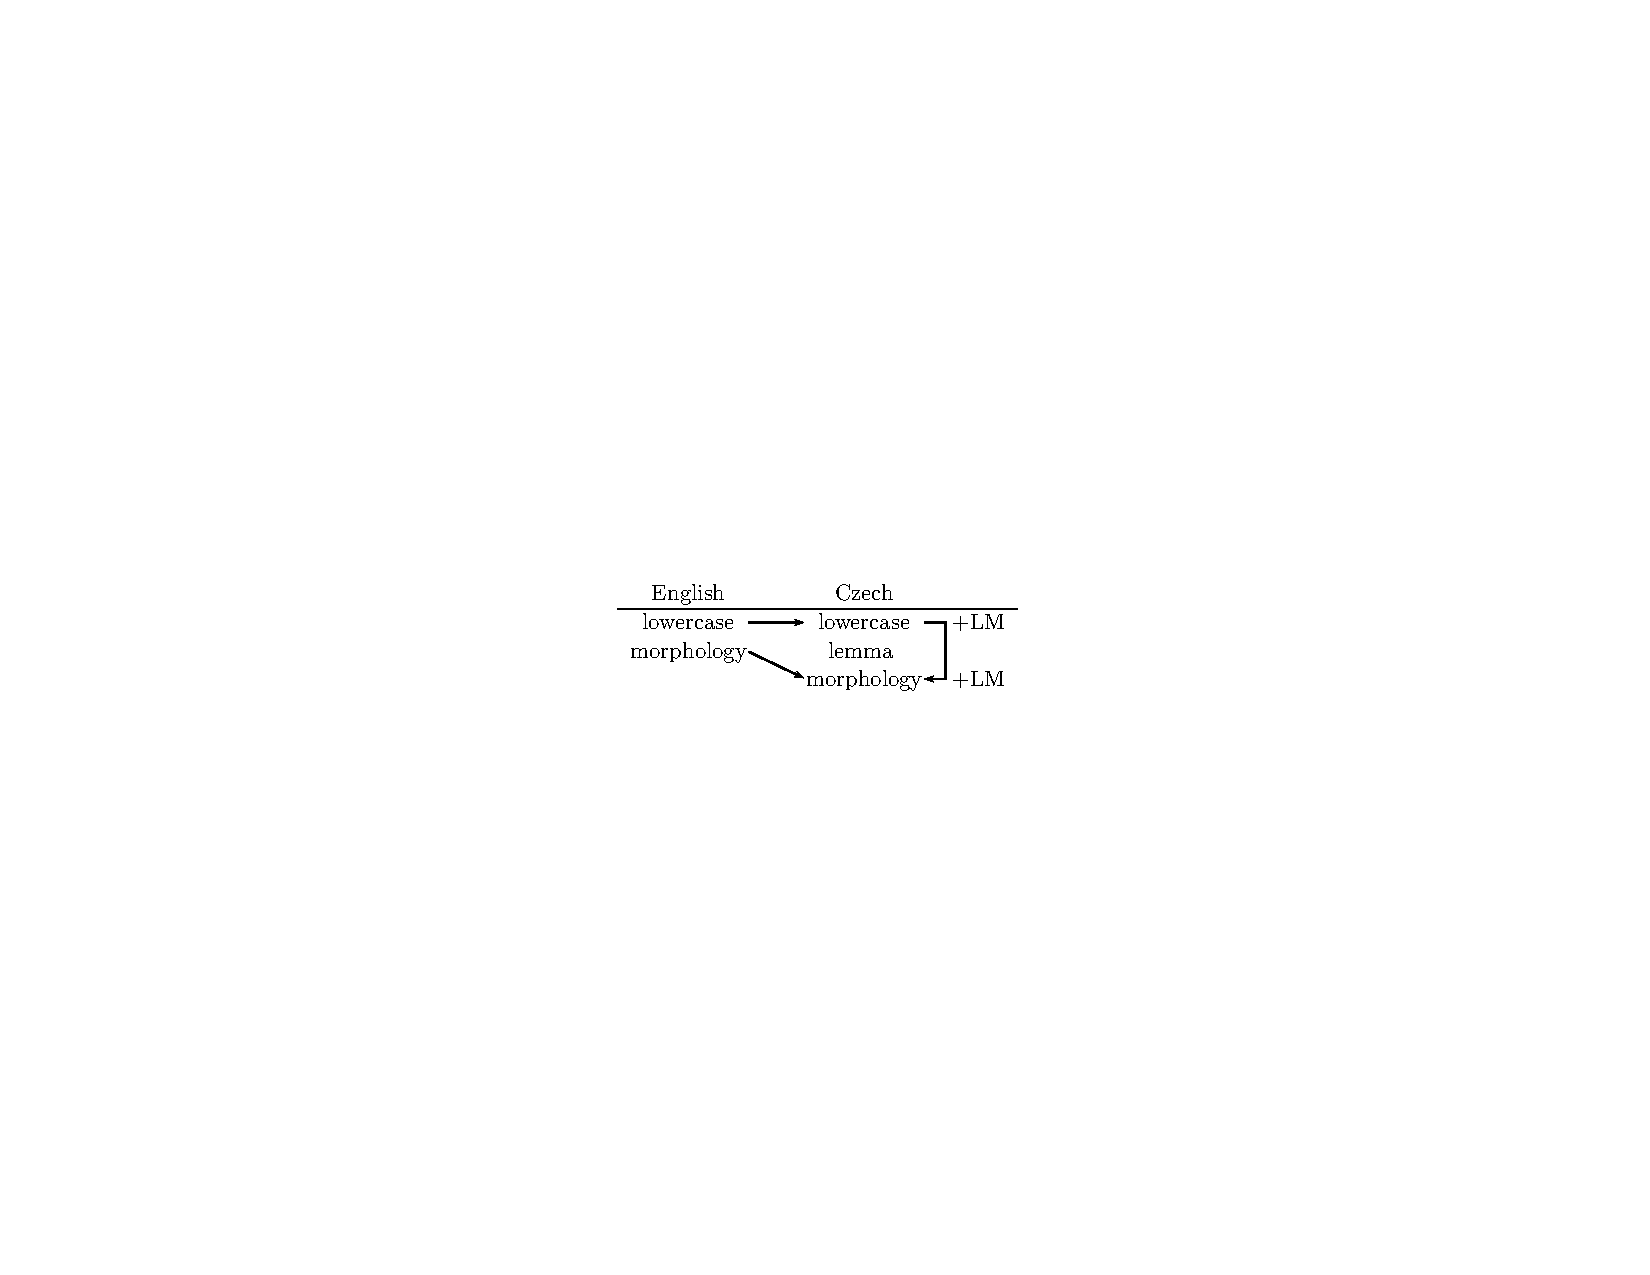
\includegraphics{images/ondrej-picture-3}
\caption{Translating and checking morphology (T+T+C).}
\end{center}
\end{figure}



As a refinement of T+C, we also used T+T+C scenario, where the morphological
output stream is constructed based on both, output word forms and input
morphology. This setting should ensure correct translation of morphological
features such as number of source noun phrases.
%, while the T+C setting simply guessed number of noun
%phrases based on the language models.

Again, two types of language models can be used in this \equo{T+T+C} scenario.

\begin{figure}
\begin{center}
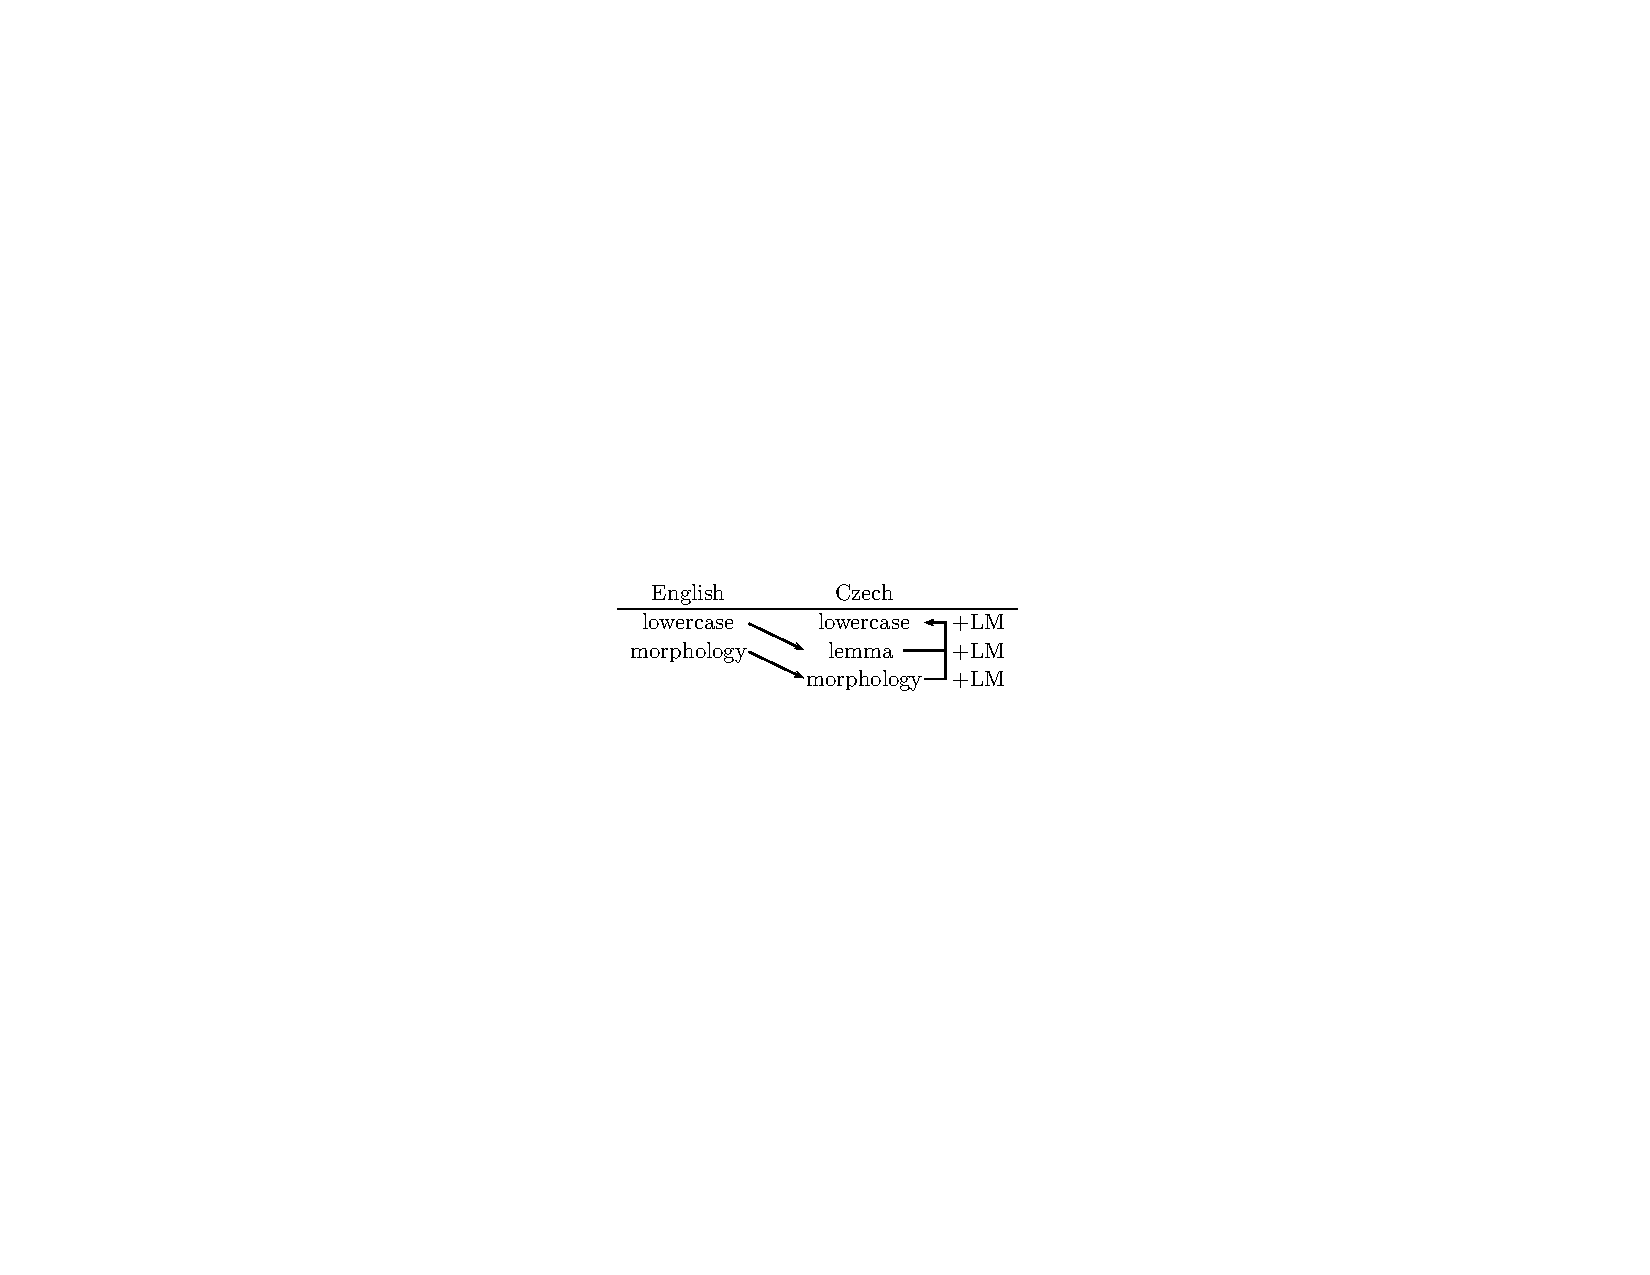
\includegraphics{images/ondrej-picture-4}
\end{center}
\caption{Generating forms from lemmas and tags (T+T+G).}
\end{figure}

The most complex scenario we used is linguistically appealing: output lemmas
(base forms) and morphological tags are generated from input in two independent
translation steps and combined in a single generation step to produce
output word forms. The input English text was not lemmatized so we used English
word forms as the source for producing Czech lemmas.

The \equo{T+T+G} setting allows us to use up to three types of language models.
Trigram models are used for word forms and lemmas and 7 or 9-gram language
models are used over tags.



%% small pictures
%\psset{unit=5mm}
%\begin{pspicture}(0,-0.5)(3,0.5)
%\psline{->}(0,0)(3,0)
%\pscircle*[fillcolor=white](0,0){0.5ex}
%\end{pspicture}
%
%\psset{unit=5mm}
%\begin{pspicture}(0,-0.5)(3,1.5)
%\psline{->}(0,1)(3,1)
%\psline{->}(3,1)(3,0)
%\end{pspicture}
%
%\psset{unit=5mm}
%\begin{pspicture}(0,-0.5)(3,2.5)
%\psline{->}(0,2)(3,2)
%\psline{->}(0,1)(3,0)
%\psline{->}(3,2)(3,0)
%\end{pspicture}
%
%
%\psset{unit=5mm}
%\begin{pspicture}(0,-0.5)(3,2.5)
%\psline{->}(0,2)(3,1)
%\psline{->}(0,1)(3,0)
%\psline{->}(3,1)(3.5,1)(3.5,2)(3,2)
%\psline{->}(3,0)(3.5,0)(3.5,2)(3,2)
%\end{pspicture}



\subsection{Results: Checking Czech morphology works}

Table \ref{scenariosresults-main} summarizes estimated translation quality of the
various scenarios. In all experiments, only the baseline corpus of 20k sentences
was used with word alignment obtained using grow-diag-final heuristic on stemmed
English and lemmatized Czech input streams. Language models are also based
on the 20k sentences only, 3-grams are used for word forms and lemmas, 7-grams
for morphological tags.


\begin{table}[ht]
\begin{center}
\begin{tabular}{lcc}
   &  Dev  &  Test \\
\hline
Baseline: T       &  29.24  &  25.23\\
T+T+G &  30.34  &  25.94\\
T+T+C  &  30.73  &  26.43\\
T+C     &  \max{30.88}  &  \max{27.23}\\
\end{tabular}
\end{center}
\caption{BLEU scores of various translation scenarios.}
\label{scenariosresults-main}
\end{table}

The good news is that multi-factored models always outperform the baseline T.
Unfortunately, the more complex a multi-factored scenario is, the worse
the results are. Our belief is that this effect is caused by search errors: with
multi-factored models, more hypotheses get similar scores and future costs
of partial hypotheses might be estimated less reliably. With the limited stack
size (not more than 200 hypotheses of the same number of covered input words),
the decoder may more often find sub-optimal solutions. The scenario for just checking output morphology (T+C) gives us the best results, 27.23 BLEU, 2 points absolute improvement over the single-factored baseline.
}

A significantly more detailed analysis of Czech translation, and a number of different experiments are presented in Appendix \ref{czech-appendix}.  

\chapter{Confusion Network Decoding}\label{chap:confusion-networks}


% Definitions.
% --------------------
\def\x{{\mathbf x}}
\def\L{{\cal L}}
\newcommand{\devfour}{{\tt dev4}}
\newcommand{\eval}{{\tt eval}}
\newcommand{\E}{{\bf e}}
\newcommand{\F}{{\bf f}}
\newcommand{\bm}[1]{{\mbox{\boldmath${#1}$}}}
\newcommand{\tf}{\tilde{f}}
\newcommand{\te}{\tilde{e}}
\newcommand{\teb}{{\bf \te}}


Machine translation input currently takes the form of simple sequences of words. However, it is desirable to integrate machine translation technology into larger information processing systems with upstream natural language processing tools (such as named entity recognizers, speech recognizers, morphological analyzers, etc.).  These upstream processes tend to generate multiple hypotheses which have varying degrees of confidence and accuracy.  Current MT systems are designed to process only one input hypothesis, making them vulnerable to errors in the input.  

One focus of our workshop was on speech translation, where the input is  generated by a speech recognizer.  Our aim was to improve performance  of spoken language translation by better integrating the output of speech recognition systems with our machine translation system.  Errors in the output of speech recognition systems can lead to compounding errors in the machine translation system, as shown in Figure~\ref{fig:wer-bleu}, which plots the Bleu scores of  translations against a speech recognizer's word error rate (WER) for the corresponding input sentences.   Rather than rely on a single transcription as input to our system, we instead will utilize a large set of transcription hypotheses generated by the speech recognition system, and combine the scores of the acoustic model, the language model, and the translation model.

Other approaches have been proposed for improving translation quality  through the processing of  multiple input hypotheses.  For instance, better translation performance 
have been reported by exploiting   $N$-best lists \citep{zhang04,quan05},  word lattices \citep{matusov05,mathias06},   and confusion networks \citep{bertoldi05a}.  
In the workshop we concentrated on {\it confusion network} decoding  
\cite{bertoldi05a},  which is simple to integrate with the translation model and can be efficiently integrated into the search algorithm.  

While the focus of this chapter is on the application of confusion networks to the problem of speech translation, the reader should note that their application to machine translation is potentially much broader.  Specifically, their inclusion in the decoder may provide a mechanism for dealing with different potential analyses of the input to the machine translation system.  This is crucially important when using other natural language processing tools to mark up input sentences for factored translation models.  

\section{Spoken language translation}
\label{sec:slt}


\begin{figure}
\begin{center}
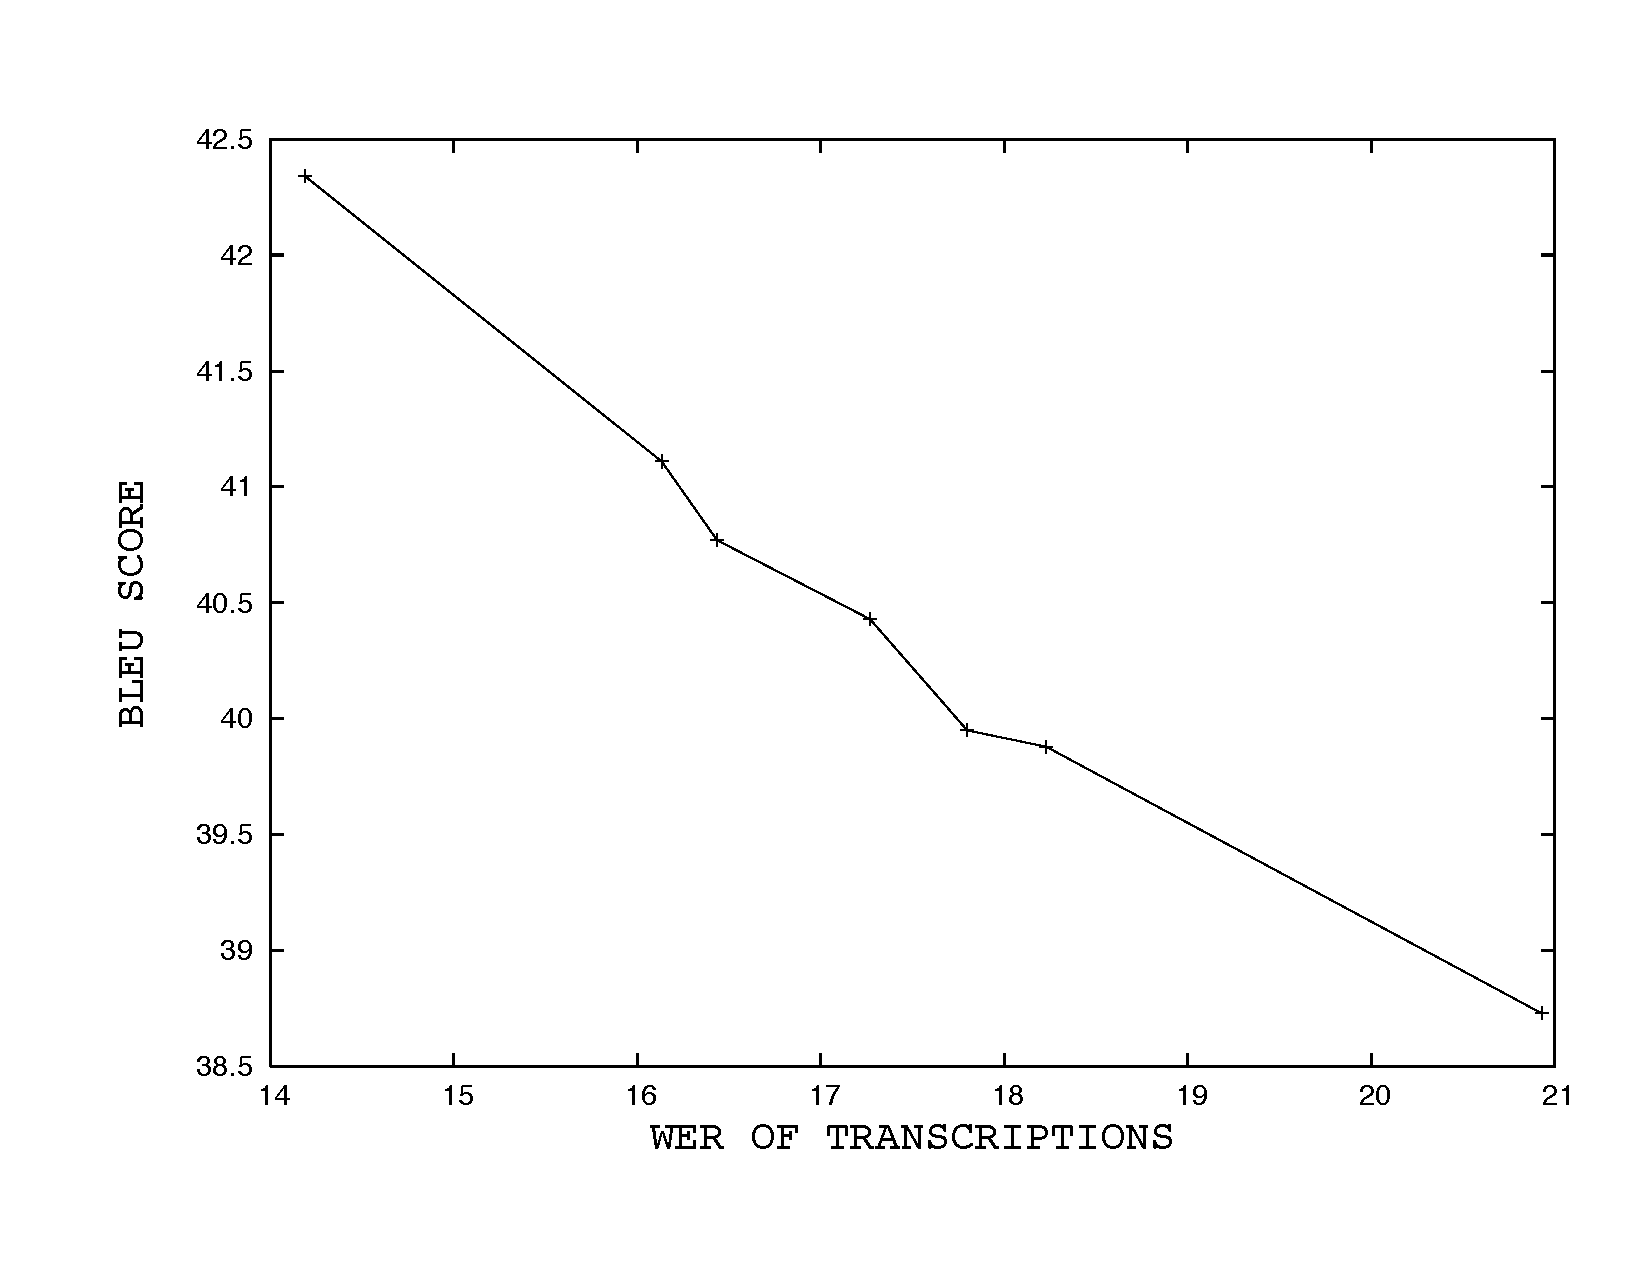
\includegraphics[width=10cm]{marcello-bleu-wer} 
\caption{Relationship between BLEU score of translations and word error rate of input sentences. Source sentences are transcriptions of parliamentary speeches produced by a speech recognition system.}
\label{fig:wer-bleu}
\end{center}
\end{figure}


Translation from speech input is considered  more difficult than  translation from text for several reasons. Spoken language has many  styles and genres, such as, formal read speech, unplanned speeches, interviews, spontaneous conversations;  it produces less controlled language, presenting more relaxed syntax and spontaneous speech phenomena. 

From a statistical perspective, SLT can be approached as follows.
Given the  vector $\o$ representing  the acoustic observations  of the
input  utterance,   let  ${\cal  F(\o)}$  be  a   set  of
transcription  hypotheses  computed by  a speech recognizers  and
represented  as a  word-graph.   The  best translation  $\E^*$ is  
searched  among all  strings in  the target language ${\cal E}$ through 
the following criterion:
%\begin{eqnarray}
\begin{equation}
%\e^* &=& \arg\max_{\E} \sum_{\f \in {\cal F}(\o)} \Pr(\E, \f  \mid \o)
\E^* = \arg\max_{\E} \sum_{\F \in {\cal F}(\o)} \Pr(\E, \F  \mid \o)
\label{eq:slt-max}
%\end{eqnarray}
\end{equation}
where the source language sentence $\F$ is an hidden variable representing any speech transcription
hypothesis.   According to the well established log-linear framework, 
 the  conditional distribution $\Pr(\E,\F  \mid \o)$ can be  determined through suitable
real-valued  feature functions  $h_r(\E,\F,\o)$  and real-valued  parameters
$\lambda_r$, $r=1\ldots R$, and takes the parametric form:
\begin{equation} 
p_{\tiny \bm{ \lambda}}(\E ,\F \mid \o) = \frac{1}{{\cal Z}(\o)} \exp\left\{ \sum_{r=1}^R \lambda_r h_r(\E,\F,\o)\right\}
\label{eq:loglin} 
\end{equation}
where ${\cal Z}(\o)$ is a normalization term.


The main advantage of the log-linear model defined in ({\ref{eq:loglin}) is
the possibility of using any kind of features, regarded as important for
the sake of translation. 
The kind of representation used for the set of hypotheses  ${\cal F}(\o)$  clearly 
impacts on the implementation  of the search algorithm. Here, we assume to 
have all hypotheses represented as a confusion network.

\section{Confusion Networks}
\label{sec:cn}

A Confusion Network (CN) ${\cal  G}$ is a weighted directed graph with
a start node, an end node, and word labels over its edges.  The CN has
the peculiarity  that each path  from the start  node to the  end node
goes    through    all    the    other    nodes.     As    shown    in
Figure~\ref{fig:CN-matrix}, a CN can be represented as a matrix of words
whose columns  have different depths.   Each word $w_{j,k}$  in ${\cal
G}$  is identified  by its  column  $j$ and  its position  $k$ in  the
column;  word   $w_{j,k}$  is  associated  to   the  weight  $p_{j,k}$
corresponding to the posterior probability $\Pr(f=w_{j,k} \mid \o, j)$
of  having  $f=w_{j,k}$ at  position  $j$  given  $\o$.  A realization 
$\F=f_1,  \ldots, f_m$ of ${\cal G}$  is associated with
the probability $\Pr(\F\mid \o)$, which is defined as follows:
\begin{equation}
\Pr (\F \mid \o)= \prod_{j=1}^m \Pr(f_j\mid \o, j)
\label{eq:CN-posterior}
\end{equation}

\begin{figure}
\begin{center}
\begin{tabular}{c|c|c|c|c}
se$_{.97}$ &  presenta$_{.40}$  & $\epsilon_{.78}$& esas$_{.86}$& elecciones$_{.97}$\\
he$_{.03}$ &  present\'o$_{.22}$  & a$_{.08}$           & $\epsilon_{.10}$& selecciones$_{.03}$\\
                     &  presentan$_{.06}$ & e$_{.07}$            & esa$_{.04}$&     \\
                       &  $\ldots$                    & en$_{.06}$          &                     &    \\
                      &                                    & $\ldots$                &                      &\\
\end{tabular}
\end{center}
\caption{Example of confusion network.}
\label{fig:CN-matrix}
\end{figure}



The  generation of  a CN  from an  ASR word-graph  \citep{mangu:00} can
also produce special empty-words $\epsilon$ in some columns. These
empty-words permit the generation of source sentences of different length and 
are treated differently from regular words only at the level of feature functions.

\subsection{Generative translation process}
\label{sec:CN-gen}

The following process describes how to incrementally generate a translation 
from a confusion network ${\cal G}$:
\bigskip


\noindent
{\tt While there are uncovered source columns}\\
 {\tt Cover a span of columns}\\
 {\tt Choose a path inside the span}\\
 {\tt Append a translation of the path to the target}\\


\subsection{CN-based log-linear model}
\label{sec:cn-model}

The log-linear model adopted for the CN decoder includes the following feature 
functions:
\begin{enumerate}
\item A word-based $n$-gram target LM.
\item A reordering model defined in terms of the distance  between the first column covered 
by current span and the last column of the previous span. (In the current implementation, we
did not distinguish between regular and empty words.)
\item Four phrase-based lexicon models exploiting statistics at word- and phrase-level. These models
remove any empty-word in the source side.
\item Phrase and word penalty models, i.e.  counts of the number of phrases and words in the target string.
\item The  CN posterior probability, see formula (\ref{eq:CN-posterior}).
\end{enumerate}

\noindent 
Notice that the above features can grouped into two categories: those which are expansion-dependent because their computation requires some knowledge about the previous step (1, 2), and those which are not (3, 4, 5).

\subsection{Decoding algorithm}
\label{sec:decoding}

According  to  the {\bold  dynamic  programming}  paradigm, the  optimal
solution can be computed through expansions and recombinations of  
previously computed  partial  theories.  With respect to translating a
single input hypothesis, translating from a CN requires, 
in principle, exploring all possible input paths inside the graph. 
A key insight is that, due to their linear structure, CN
decoding is very similar to text decoding.  During the
decoding, we have to look up the translation options of spans, i.e. some
contiguous sequence of source positions.  The main
difference between CN and text decoding is that in text
decoding there is exactly one source phrase per span, whereas in
confusion network decoding there can be multiple source phrases per
span.  In fact, in a CN the number of source phrases
per span is exponential in the span length, assuming its minimum depth is larger than one.


The decoding algorithm can be made much more efficient by 
pre-fetching translations for all the spans and by applying  early recombination. 

\subsection{Early recombination}
\label{sec:early-rec}

At each expansion step  a span covering a given number of consecutive columns is generated. 
Due to the presence of empty-words, different paths within the span can 
generate the same source phrase, hence the same translations. The scores of such 
paths only impacts the CN posterior feature (5).  Additionally, it might happen that two 
different source phrases of the same span have a common translation. In this case, not only the CN 
posterior feature is different, but also the phrase translation features (3).
This  suggests that efficiency can be gained by pre-computing all possible alternative
 translations for all possible spans, together with their expansion-independent scores, 
 and to recombine these translations in advance.  
  
\subsection{Pre-fetching of translation options} 
\label{sec:pre-fetching}

Concerning the pre-fetching of translations from the phrase-table, an 
efficient implementation can be achieved if we use a prefix
tree representation for the source phrases in the phrase table and
generate the translation options incrementally over the span length.
So, when looking up a span $(j_1,j_2)$, we can exploit our knowledge
about the span $(j_1,j_2-1)$.  Thus, we have to check only for the
known prefixes of $(j_1,j_2-1)$ if there exists a successor prefix
with a word in column $j_2$ of the CN.  If all the word
sequences in the CN also occur in the phrase table,
this approach still enumerates an exponential number of phrases.  So,
the worst case complexity is still exponential in the span length.
Nevertheless, this is unlikely to happen in practice.  In our
experiments, we do not observe the exponential behavior.  What we
observe is a constant overhead compared to text input.



\section{$N$-best decoder}

A widely used  approach in spoken language translation  is 
the N-best  translation, which we used as a baseline for comparison in our experiments.

\bigskip
\label{sec:1best-smt}

An alternative way to define the set ${\cal F}(\o)$ is to take the $N$
most  probable hypotheses  computed by  the ASR  system,  i.e.  ${\cal
F}(\o)=\{\F_1, \ldots,\F_N\}$. By  taking a maximum approximation over
${\cal F}(\o)$, and assuming that $\Pr(\teb, \F \mid \o) = \Pr(\F\mid
\o)   \Pr(\teb   \mid  \F)$, we get the search criterion:
\begin{eqnarray}
\label{eq:nbest-max-1}
\teb^* &\approx& \arg\max_{n=1,..,N}    \Pr(\F_n \mid \o) \max_{\teb} \Pr(\teb \mid \F_n)
\label{eq:nbest-max}
\end{eqnarray}


In the equation above we can isolate $N$ independent translation tasks 
(rightmost  maximization),  and   the  recombination  of  their  results
(leftmost maximization).  Hence, the search criterion  can be restated
as:
\begin{eqnarray}
\teb_n^* &=& \arg\max_{\teb} \Pr(\teb \mid \F_n)    \qquad n=1,\ldots, N \\
\teb^* &\approx& \arg\max_{n=1,..,N} \Pr(\F_n  \mid \o) \Pr(\teb_n^* \mid \F_n)
\label{eq:nbest-max-alg}
\end{eqnarray}


In other words: the best translation $\teb_n^*$ of each
transcription hypothesis $\F_n$ is found; then, the best
translation $\teb^*$ is selected among $\{\teb_1^*, \ldots,
\teb_N^*\}$ according to its score weighted by the ASR posterior
probability $\Pr(\F_n \mid \o)$.


In the experimental chapters we will compare performance of the CN decoder against the above N-best approach.


\chapter{Experiments with Confusion Nets}\label{confusion-net-experiments}




\section{Results for the BTEC Task}

The experiments were carried out on the {\it Basic Travel Expression Corpus} (BTEC) task \cite{takezawa02}. 
This is a multilingual speech corpus which contains tourism-related sentences similar to those that are found in phrase books.
The corpus statistics are shown in Table~\ref{tab-corpus}.
For the supplied data track, 40\,000 sentences training corpus and three test sets were made available for each language pair.

\begin{table}
\begin{center}
\caption{Corpus statistics for the Chinese-English task.} \label{tab-corpus}
\begin{tabular}{|l|r|r|}
\hline
& Chinese & English \\
\hline
sentences & \multicolumn{2}{c|}{40 K} \\ \cline{2-3}
running words & 351 K  &  365 K \\
avg. sent. length& 8.8& 9.1 \\
vocabulary entries& 11 K & 10 K \\
\hline
\end{tabular}
\end{center}
\end{table}

%As the BTEC is a rather clean corpus, the preprocessing consisted mainly of tokenization, i.e., separating punctuation marks from words.
%Additionally, we replaced  contractions such as {\bold it's} or {\bold I'm} in the English corpus and we removed the case information.
%There was no special preprocessing for the Chinese and the Japanese training corpora.


\subsection{Chinese-to-English}

In this section, we will present the experimental results for the Chinese--English task.
The statistics of the confusion networks are summarized in Table~\ref{tab-ce-cn-stat}.
Note that the average length of the sentences in the \devfour\ test set is about twice as large as in the training data.
We also present the depths of the confusion networks. %, i.e. the number of alternatives per position.
On average we have  between two and three alternatives per position.
At some positions, however, there are more than 90 alternatives.
\begin{table}[t]
\begin{center}
\caption{Chinese--English: confusion network statistics for the \devfour\ test set (489 sentences).} \label{tab-ce-cn-stat}
\begin{tabular}{|l|r|r|}
\cline{2-3}
\multicolumn{1}{c}{}&\multicolumn{2}{|c|}{speech type} \\ \hline
& read  & spontaneous  \\
\hline
avg. length & 17.2 & 17.4 \\
avg. / max.  depth & 2.2  / 92 & 2.9 / 82  \\
avg. number of paths & $10^{21}$ & $10^{32}$ \\
\hline
\end{tabular}
\end{center}
\end{table}


In Table~\ref{tab-ce-cn-results}, we present the translation results for the Chinese--English task for different input conditions on the \devfour\ and the \eval\ test sets.
Comparing the translation results of 1-best and confusion network, we observe a small but consistent improvement for read speech.
For spontaneous speech, the improvements are larger, e.g. 1.1\% BLEU for the \eval\ test set.

\begin{table}[t]
\begin{center}
\caption{Chinese--English: translation results for different input types.} \label{tab-ce-cn-results}
\begin{tabular}{|c|l|c|c|}
\cline{3-4}
\multicolumn{2}{c}{}&\multicolumn{2}{|c|}{speech type} \\
\hline
test  && read  & spontaneous \\
set &input& BLEU [\%] & BLEU [\%] \\
\hline \hline
\devfour & verbatim & \multicolumn{2}{c|}{21.4} \\ \cline{2-4}
& 1-best  & 19.0 & 17.2 \\ 
\cline{2-4}
& full CN & 19.3 & 17.8 \\
\hline 
 \hline
 \eval & verbatim & \multicolumn{2}{c|}{21.4} \\ \cline{2-4}
 & 1-best  & 18.5 & 17.0 \\ 
\cline{2-4}
& full CN & 18.6 & 18.1 \\
\hline 
\end{tabular}
\end{center}
\end{table}
	
\section{Results for the EPPS Task}
Additional experiments for confusion network decoding were carried out on the Spanish-to-English EPPS (European Parliament Plenary Sessions) task.
The training data was collected within the TC-Star project\footnote{http://www.tc-star.org} and is a superset of the Spanish--English EuroParl corpus (\cite{koe:05}).


\subsection{Corpus Statistics}
Statistics for this task are reported in Table~\ref{tbl:epps-corpstat}.  
The bilingual training corpus consists of about 1.3\,M sentence pairs with about 36\,M running words in each language.
The training was performed with the {\tt Moses} training tools, while training of the 4-gram target LM was performed with the IRST LM Toolkit.
Sentences in the dev and test sets are provided with two reference translations each.  
\begin{table}[t]
\begin{center}
\caption{Corpus statistics for the Spanish-English EPPS task.
% For development and test sets, figures related to Spanish refer to {\tt verbatim} input type, whereas figures related to English refer to the reference translations.
} \label{tbl:epps-corpstat}
\begin{tabular}{|l|l|r|r|}
 \hline
       &              &  Spanish   &   English     \\
\hline
Train  & Sentences    & \multicolumn{2}{c|}{1.3\,M}\\
\cline{2-4}
      & Words & 37\,M & 36\,M\\
\cline{2-4}
       & Vocabulary   & 143\,K & 110\,K\\
\cline{2-4}
       & Phrase Pairs   & \multicolumn{2}{c|}{83\,M}\\
\cline{2-4}
       & Phrases   & 48\,M & 44\,M\\
 \hline
Dev    & Utterances    &   \multicolumn{2}{c|}{2\,643} \\
 \cline{2-4}
       & Words& 20\,384 & 20\,579 \\ 
%\cline{2-4}
%       & Vocabulary   & 2\,883 &  2\,362 \\
 \hline
Test   & Utterances    & \multicolumn{2}{c|}{1\,073}  \\
 \cline{2-4}
       & Words& 18\,890 & 18\,758 \\
 \cline{2-4}
 %      & Vocabulary   & 3\,139 & 2\,567 \\
 %\cline{2-4}
%       & OOV Words & 145 & 44\\
 \hline
\end{tabular}
\end{center}
\end{table}


The ASR word lattices  were  kindly provided by CNRS-LIMSI, France.
The confusion networks and $N$-best lists were extracted using the {\tt lattice-tool} included in the SRILM Toolkit (\cite{stolcke:02}). 
%The consensus decoding transcriptions  were also extracted from the confusion networks, by taking the most probable words from  each column.
The statistics of the confusion networks for the Spanish--English EPPS task are presented in Table~\ref{tbl:epps-cn}.
The average depth of the confusion networks, i.e. the average number of alternatives per position, is 2.8 for the development set and 2.7 for the test set.
Note that the maximum depth is much larger, e.g. up to 165 for the development set.
Also, the average number of paths in the confusion networks is huge. 

\begin{table}[t]	
	\caption{Statistics of the confusion networks for the development and test sets of the Spanish--English EPPS task.}\label{tbl:epps-cn}
	\begin{center}
	\begin{tabular}{|l|r|r|}
	\hline
	& Dev & Test \\
	\hline
	Utterances & 2\,633  & 1\,071 \\
	Avg. length & 10.6 &  23.6 \\
	Avg. / max.  depth & 2.8  / 165 & 2.7 / 136  \\
	Avg. number of paths & $10^{38}$ & $10^{75}$ \\
	\hline
	\end{tabular}
	\end{center}
\end{table}


\subsection{Parameter Tuning}
The feature  weights of all models were optimized using minimum-error-rate training (\cite{Och2003c}) which tries to maximize the BLEU score on the development set.  
A special procedure was used for tuning the weights of the $N$-best translation system. 
First, a single best decoder was optimized over the development set. 
Then $M$-best translations were generated for each $N$-best input of the development set. 
Hence, all $N$x$M$ translations were merged and a new log-linear model  including the ASR additional features was trained. 


\subsection{Translation Results}

\begin{table}[t]
\caption{Translation performance achieved by {\tt Moses} for different input types for the test set of the Spanish--English EPPS task.}
\begin{center}
\begin{tabular}{|l|l||c||ccc|}
 %\hline
%\multicolumn{2}{|c|}{Input} &\multicolumn{3}{c|}{MT Quality}  \\
\hline
\multicolumn{2}{|c||}{Input Type}                & ASR WER [\%]     & BLEU [\%] 	& PER [\%] 	& WER [\%] \\
\hline \hline
\multicolumn{2}{|c||}{{\tt verbatim}}   & \phantom{0}0.00      & 48.00 & 31.19 & 40.96 \\
 \hline \hline
%{\tt oracle from wg} &\phantom{0}7.48     & 44.68 & 33.55 & 43.74 \\ 
%{\tt \phantom{oracle from} cn}  &\phantom{0}8.45     & 44.12 & 34.37 & 44.95 \\
 %\hline
ASR & {\tt 1-best, wg}        & 22.41 & 37.57 & 39.24 & 50.01 \\
&{\tt \phantom{1-best,} cn}  & 23.30  & 36.98 & 39.17 & 49.98  \\
 \cline{2-6}
&{\tt cn}               &\phantom{0}8.45     & 39.17 & 38.64 & 49.52 \\
 \cline{2-6}
&{\tt N-best, N=1}        & 22.41 & 37.57 & 39.24 & 50.01 \\
%{\tt 5-best}*      & 18.61 & 38.96 & 38.78 & 49.40 \\
&{\tt \phantom{N-best,} N=5}        & 18.61 & 38.68 & 38.55 & 49.33 \\
%{\tt 10-best}*    & 17.12 & 38.71 & 38.74 & 49.29 \\
&{\tt \phantom{N-best,} N=10}      & 17.12 & 38.61 & 38.69 & 49.46 \\
 \hline
 \end{tabular}
\end{center}
\label{tbl:epps-results}
\end{table}


In Table~\ref{tbl:epps-results}, we report the translation performance for different input types:
\begin{itemize}
\item {\tt verbatim}: These are the translation results for the correct transcriptions of the speech signal. Therefore, the ASR word error rate is 0.0\% for this input type.
%\item {\tt oracle}: These are the translation results for the best ASR transcriptions contained in the word graphs ({\tt wg}) and the confusion networks ({\tt cn}), respectively. 
\item {\tt 1-best}: Here, we have translated the single-best ASR transcription of the word graphs ({\tt wg}) and the confusion networks ({\tt cn}), respectively.
\item {\tt cn}: These are the results for decoding the full confusion networks.
\item {\tt N-best}: These are the results for $N$-best decoding with $N=1,5,10$.
\end{itemize}
The optimization of the system was performed separately for each input type, as described before.
In addition to the translation results, we also report the ASR word error rate.
Note that for the confusion network ({\tt cn}) and the $N$-best lists ({\tt N-best}) input types,  we reported the ASR WER of the best transcription contained in the confusion network or the $N$-best lists, respectively.
The comparison of the scores for the different input conditions %on the text inputs ({\tt verbatim}, {\tt wg-oracle}, {\tt cn-oracle}, {\tt 1-best}, and {\tt cons-dec})
shows a strong correlation between quality of the transcriptions given by the ASR WER and quality of the translation given by the MT scores.

Assuming a perfect ASR system, i.e. in the {\tt verbatim} condition, we achieve a BLEU score of 48\%.
Comparing this to the ASR input conditions, we observe a degradation of about 10 BLEU points in the case of ASR input.

The confusion network decoding ({\tt cn}) achieves the best BLEU score among the ASR input types. %, i.e. for all input types except {\tt verbatim}.
Note the large gain compared to the single-best input types, e.g. 1.6\% BLEU absolute over the single-best from the word graphs and even more over the single-best from the confusion networks.

In terms of WER and PER, the {\tt 5-best} system is slightly better.
%The translation of confusion networks ({\tt cn}) outperforms the translation of all  $N$-best lists with respect to BLEU, and only the translation of 1-best with respect to PER and WER. 
This could be due to the fact that the systems were optimized for BLEU.

\subsection{Efficiency}

Experimentally, the ratio between the decoding time for translating the confusion networks ({\tt cn}) and the single-best ({\tt 1-best}) is about 2.1 (87.5 vs 42.5 seconds per sentence). 
As the decoding time for $N$-best lists is proportional to $N$, we can claim that decoding CNs  is preferrable to translating $N$-best ($N>2$) with respect to translation speed, i.e. decoding confusion networks is more efficient than translating $N$-best lists.


In Figure~\ref{fig-cn-exploration}, we show the effect of the incremental pre-fetching of translation options for confusion network decoding.
The curve labeled 'CN total', represents the total number of paths in the confusion networks as a function of the path length.
This is the number of phrases enumerated using a naive pre-fetching algorithm.
Note the exponential growth with increasing path length.
Therefore, the naive algorithm is only applicable for very short phrases and heavily pruned confusion networks.
\begin{figure} 
	\begin{center}
		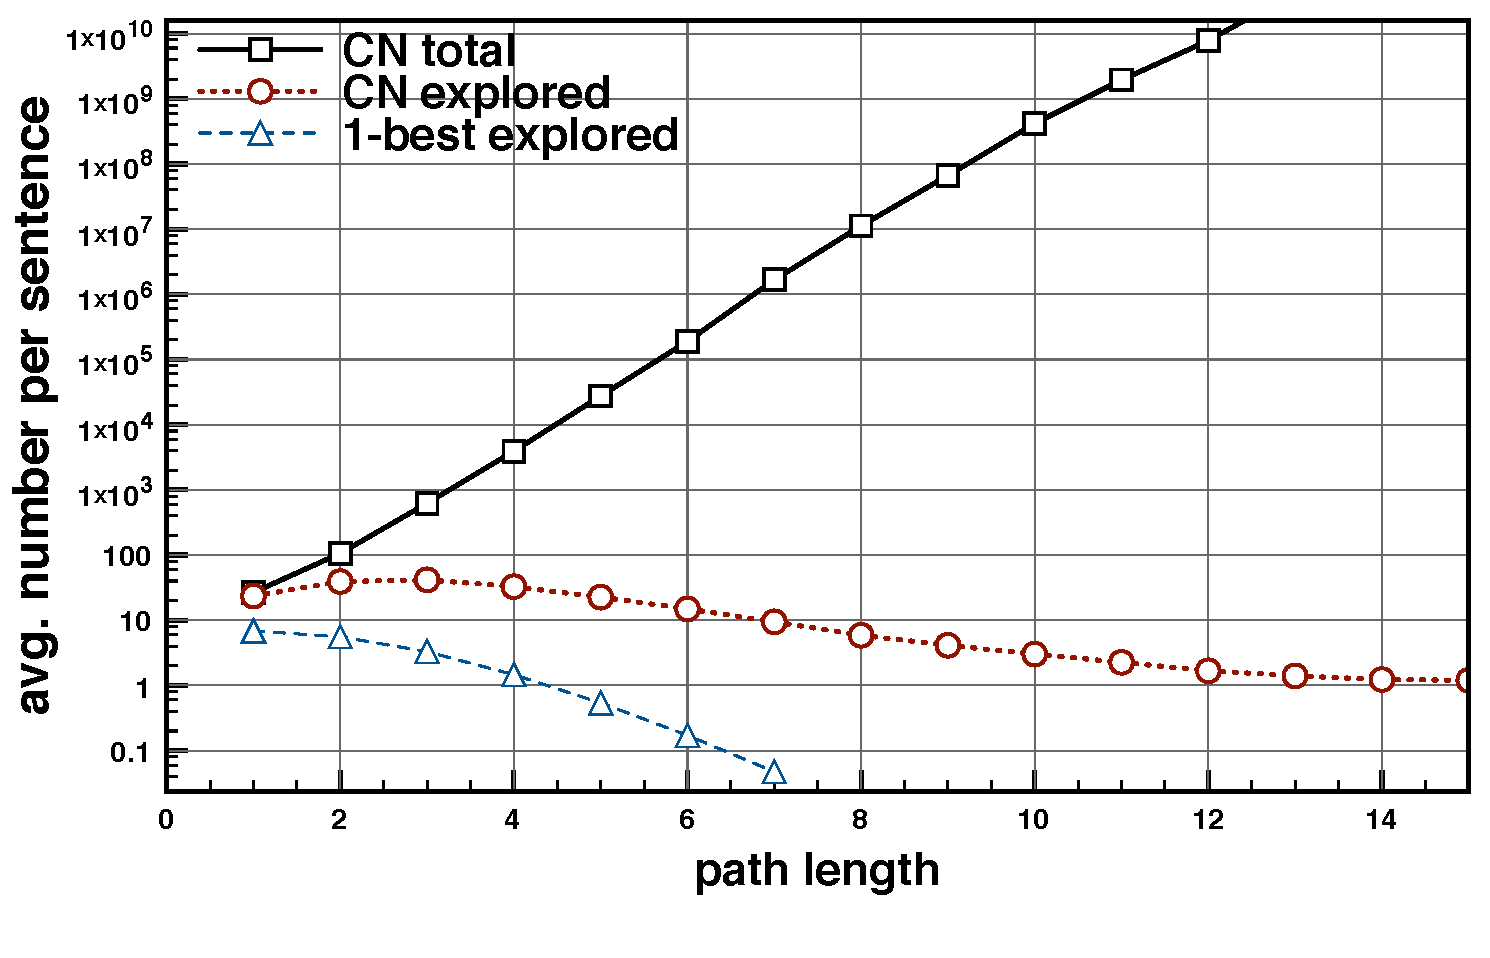
\includegraphics[width=0.75\linewidth]{CN_PathExploration}
		\caption{Exploration of the confusion networks for the Spanish--English EPPS task.}\label{fig-cn-exploration}
	\end{center}
\end{figure}
The next curve, labeled 'CN explored', is the number of paths that are actually explored using the incremental algorithm described in Section~\ref{sec:pre-fetching}.
We do {\bold not} observe the exponential explosion as for the total number of paths.
%Thus, the presented algorithm effectively solves the combinatorial problem of matching phrases of the input \CN s and the phrase table.
For comparison, we also plotted the number of explored paths for the case of single-best input, labeled '1-best explored'.
The maximum phrase length in the phrase table for  these experiments is seven.
In the case of confusion network input, this length can be exceeded as the confusion networks may contain $\epsilon$-transitions.





\chapter{Open Source Toolkit}\label{toolkit}


%\begin{quote}
%    \texttt{http://sourceforge.net/projects/mosesdecoder/}
%\end{quote}


\section{Overall design}
In developing the Moses decoder we were aware that the system should be open-sourced if it were to gain the support and interest from the machine translation community that we had hoped. There were already several proprietary decoders available which frustrated the community as the details of their algorithms could not be analysed or changed.
However, making the source freely available is not enough. The decoder must also advance the state-of-the-art in machine translation to be of interest to other researchers. Its translation quality and runtime resource consumption must be comparable with the best available decoders. Also, as far as possible, it should be compatible with current systems which minimize the learning curve for people who wish to migrate to Moses. 
We therefore kept to the following principles when developing Moses:
\begin{itemize}	
 \item Accessibility 
 \item 	Easy to Maintain
 \item	Flexibility
 \item	Easy for distributed team development
 \item	Portability
\end{itemize}

By adding factored translation to conventional phrase based decoding we hope to incorporate linguistic information into the translation process in order to create a competitive system.

Resource consumption is of great importance to researchers as it often determine whether or not experiments can be run or what compromises needs to be taken. We therefore also benchmarked resource usage against another phrase-based decoder, Pharaoh, as well as other decoders, to ensure that they were comparable in like-for-like decoding.

It is essential that features can be easily added, changed or replace, and that the decoder can be used as a ‘toolkit’ in ways not originally envisaged. We followed strict object oriented methodology; all functionality was abstracted into classes which can be more readily changed and extended. For example, we have two implementations of single factor language models which can be used depending on the functionality and licensing terms required. Other implementations for very large and distributed LMs are in the pipeline and can easily be integrated into Moses. The framework also allows for factored LMs; a joint factor and skipping LM are currently available.

\begin{figure}[h]
\begin{center}
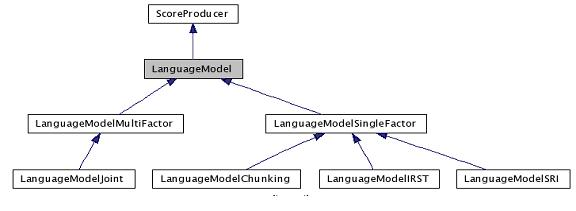
\includegraphics[scale=1]{hieu-2}
\end{center}
\caption{Language Model Framework}
\end{figure}

Another example is the extension of Moses to accept confusion networks as input. This also required changes to the decoding mechanism.

\begin{figure}[h]
\begin{center}
\centering
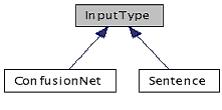
\includegraphics[scale=1]{hieu-3}
\end{center}
\caption{Input}
\end{figure}

\begin{figure}[h]
\begin{center}
\centering
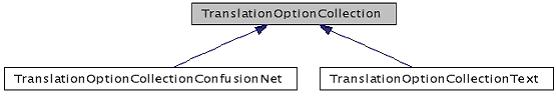
\includegraphics[scale=0.8]{hieu-4}
\caption{Translation Option Collection}
\end{center}
\end{figure}

Nevertheless, there will be occasions when changes need to be made which are unforeseen and unprepared. In these cases, the coding practices and styles we instigated should help, ensuring that the source code is clear, modular and consistent to enable the developers to quickly assess the algorithms and dependencies of any classes or functions that they may need to change.

A major change was implemented when we decided to collect all the score keeping information and functionality into one place. That this was implemented relatively painlessly must be partly due to the clarity of the source code.

\begin{figure}[h]
\begin{center}
\centering
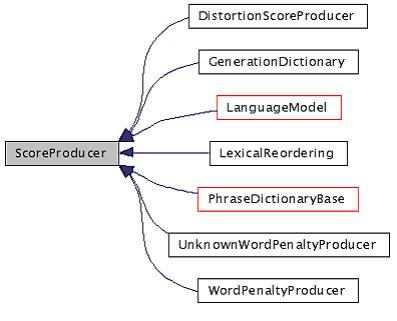
\includegraphics[scale=0.8]{hieu-5}
\caption{Scoring framework}
\end{center}
\end{figure}

The decoder is packaged as a library to enable users to more easily comply with the LGPL license. The library can also be embedded in other programs, for example a GUI front-end or an integrated speech to text translator.

\subsection{Entry Point to Moses library}

The main entry point to the library is the class\\
\indent{\tt Manager}\\
\\
For each sentence or confusion network to be decoded, this class is instantiated and the following function called\\
\indent{\tt ProcessSentence()}\\
\\
Its outline is shown below\\
\begin{tt}
\indent CreateTranslationOptions()\\
\indent for each stack in m\_hypoStack\\
\indent \indent prune stack\\
\indent \indent for each hypothesis in stack\\
\indent \indent \indent ProcessOneHypothesis()\\
\end{tt}\\
Each contiguous word coverage ("span") of the source sentence is analysed in\\ 
\indent {\tt CreateTranslationOptions() }\\
\\
and translations are created for that span. Then each hypothesis in each stack is processed in a loop. This loop starts with the stack where nothing has been translated which has been initialised with one empty hypothesis.
\\
\subsection{Creating Translations for Spans}
The outline of the function \\
\indent {\tt TranslationOptionCollection::CreateTranslationOptions()}

is as follows:\\
\begin{tt}
\indent	for each span of the source input\\
\indent \indent	CreateTranslationOptionsForRange(span)\\
\indent	ProcessUnknownWord()\\
\indent	Prune()\\
\indent	CalcFutureScoreMatrix()
\end{tt}

A translation option is a pre-processed translation of the source span, taking into account all the translation and generation steps required. Translations options are created in\\
\indent {\tt CreateTranslationOptionsForRange()}

which is out follows\\
\begin{tt}
\indent	ProcessInitialTranslation()\\
\indent	for every subequent decoding step\\
\indent \indent	if step is ‘Translation’\\
\indent \indent \indent	DecodeStepTranslation::Process()\\
\indent \indent else if step is ‘Generation’\\
\indent \indent \indent DecodeStepGeneration::Process()\\
\indent Store translation options for use by decoder\\
\end{tt}

However, each decoding step, whether translation or generation, is a subclass of\\
\indent {\tt DecodeStep}

so that the correct Process() is selected by polymorphism rather than using if statements as outlined above.


\subsection{Unknown Word Processing}
After translation options have been created for all contiguous spans, some positions may not have any translation options which covers it. In these cases, CreateTranslationOptionsForRange() is called again but the table limits on phrase and generation tables are ignored.

If this still fails to cover the position, then a new target word is create by copying the string for each factor from the untranslatable source word, or the string "UNK" if the source factor is null.

\begin{center}
\begin{tabular}{|c|c|c|}
\hline
Source Word & & New Target Word \\ \hline
Jimmy	& 	$\to$	& Jimmy\\
Proper Noun	& $\to$	& Proper Noun\\
-	& $\to$	& UNK\\
-	& $\to$	& UNK\\ \hline
\end{tabular}
\end{center}

This algorithm is suitable for proper nouns and numbers, which are one of the main causes of unknown words, but is incorrect for rare conjugation of source words which have not been seen in the training corpus. The algorithm also assumes that the factor set are the same for both source and target language, for instance, th list of POS tags are the same for source and target. This is clearly not the case for the majority of language pairs. Language dependent processing of unknown words, perhaps based on morphology. is a subject of debate for inclusion into Moses.

Unknown word processing is also dependent on the input type - either sentences or confusion networks. This is handled by polymorphism, the call stack is\\
\begin{tt}
\indent	Base::ProcessUnknownWord()\\
\indent \indent	Inherited::ProcessUnknownWord(position)\\
\indent \indent \indent	Base::ProcessOneUnknownWord()\\
\end{tt}

where\\
\indent {\tt Inherited::ProcessUnknownWord(position)}\\

is dependent on the input type.

\subsection{Scoring}
A class is created which inherits from\\
\indent {\tt ScoreProducer}

for each scoring model. Moses currently uses the following scoring models:\\
\begin{center}
\begin{tabular}{|r|r|}
\hline
$ Scoring model $&$ Class $\\
\hline
Distortion	& DistortionScoreProducer\\
WordPenalty	& WordPenaltyProducer\\
Translation	& PhraseDictionary\\
Generation	& GenerationDictionary\\
LanguageModel	& LanguageModel\\
\hline
\end{tabular}
\end{center}

The scoring framework includes the classes \\
\begin{tt}
\indent ScoreIndexManager\\
\indent	ScoreComponentCollection
\end{tt}

which takes care of maintaining and combining the scores from the different models for each hypothesis.

\subsection{Hypothesis}
A hypothesis represents a complete or incomplete translation of the source. Its main properties are

\begin{center}
\begin{tabular}{|r|l|}
\hline
$ Variables $&$ $\\
\hline
m\_sourceCompleted & Which source words have already been translated\\
m\_currSourceWordsRange & Source span current being translated\\
m\_targetPhrase & Target phrase currently being used\\
m\_prevHypo & Pointer to preceding hypothesis that translated \\
 & the other words, not including m\_currSourceWordsRange\\
m\_scoreBreakdown & Scores of each scoring model\\
m\_arcList & List of equivalent hypothesis which have lower\\
 & score than current hypothesis\\
\hline
\end{tabular}
\end{center}

Hypothesis are created by calling the constructor with the preceding hypothesis and an appropriate translation option. The constructors have been wrapped with static functions, Create(), to make use of a memory pool of hypotheses for performance.

Many of the functionality in the Hypothesis class are for scoring. The outline call stack for this is\\
\begin{tt}
\indent CalcScore()\\
\indent	\indent	CalcDistortionScore()\\
\indent	\indent	CalcLMScore()\\
\indent	\indent	CalcFutureScore()\\
\end{tt}

The Hypothesis class also contains functions for recombination with other hypotheses. Before a hypothesis is added to a decoding stack, it is compare to other other hypotheses on the stack. If they have translated the same source words and the last n-words for each target factor are the same (where n is determined by the language models on that factor), then only the best scoring hypothesis will be kept. The losing hypothesis may be used latter when generating the n-best list but it is otherwise not used for creating the best translation.

In practise, language models often backoff to lower n-gram than the context words they are given. Where it is available, we use information on the backoff to more agressively recombine hypotheses, potentially speeding up the decoding.

The hypothesis comparison is evaluated in \\
\indent {\tt NGramCompare()}

while the recombination is processed in the hypothesis stack class\\
\indent {\tt HypothesisCollection::AddPrune()}

and in the comparison functor class\\
\indent {\tt HypothesisRecombinationOrderer}


\subsection{Phrase Tables}	
The main function of the phrase table is to look up target phrases give a source phrase, encapsulated in the function\\
\indent {\tt PhraseDictionary::GetTargetPhraseCollection()}

There are currently two implementation of the PhraseDictionary class

\begin{tabular}{|l|l|}
\hline
PhraseDictionaryMemory & Based on std::map. Phrase table loaded\\ 
 & completely and held in memory\\
PhraseDictionaryTreeAdaptor & Binarized phrase table held on disk and \\
 & loaded on demand.\\
\hline
\end{tabular}

\subsection{Command Line Interface}
The subproject, moses-cmd, is a user of the Moses library and provides an illustration on how the library functions should be called. 

However, since most researchers will be using a command line program for running experiments, it will remain the defacto Moses application for the time being.

Apart from the main() function, there are two classes which inherites from the moses abstract class, InputOutput:\\
\indent {\tt	IOCommandLine}\\
\indent {\tt	IOFile (inherites from IOCommandLine)}

These implement the required functions to read and write input and output (sentences and confusion network inputs, target phrases and n-best lists) from standard io or files.

\section{Software Engineering Aspects}

\subsection{Regression Tests}
Moses includes a suite of regression tests designed to ensure that
behavior that has been previously determined to be correct does not
break when new functionality is added, when bugs are fixed, or when performance
improvements are made. The baseline behavior for the regression
testing is determined in three ways:
\begin{enumerate}
  \item Expected behavior based on off-line calculations (for example,
  given a small phrase table and sample input, one can work through
  the search space manually and compute the expected scores for a translation hypothesis).
  \item Expected values based on comparisons with other systems (for
  example, language modeling toolkits provide the ability to score
  a sentence.  Such a tool can be used to calculate the expected value of
  the language model score that will be produced by the decoder).
  \item Expected values based on previous behavior of the decoder (some output behavior
  is so complex that it is impractical or impossible to determine externally
  what the expected values are; however, it is reasonable to assume that localized bug-fixes,
  the addition of new functionality, or performance improvements should not impact existing
  behavior).
\end{enumerate}
The nature of statistical machine translation decoding makes
achieving substantial and adequate test coverage possible with
simple black-box testing.  Aggregate statistics on the number of
hypotheses generated, pruned, explored, as well as comparisons of
the exact costs and translations for certain sample sentences
provide ample evidence that the models and code that is utilized in
decoding is working adequately since these values tend to be highly
sensitive to even minor changes in behavior.

\subsubsection{How it works}
The test harness (invoked with the command \texttt{run-test-suite})
runs the decoder that is to be tested (specified to the script with
the \texttt{--decoder} command line option) with a series of
configuration files and translation inputs.  The output from the
decoder, which is written to \texttt{stdout} and \texttt{stderr}, is
post-processed by small scripts that pull out the data that is going
to be compared for testing purposes.  These values are compared with
the baseline and a summary is generated.

Timing information is also provided so that changes that have
serious performance implications can be identified as they are made.
This information is dependent on a variety of factors (system load,
disk speed), so it is only useful as a rough estimate.

\subsubsection{Versioning}
The code for the regression test suite is in the
\texttt{regression/tests} subdirectory of the Subversion repository.
 The inputs and expected values for each test case in the test suite are stored
together in \texttt{regression-tests/tests}.  The test suite is
versioned together with the source code for several reasons:
\begin{enumerate}
  \item As bugs are identified and fixed that change existing behavior, the
testing code needs to be updated.
  \item As new functionality is added, testing code exercising this functionality needs to be
  added.
\end{enumerate}
By versioning the regression tests together with the source code, it
should be possible to minimize when developers need to worry about
expected test failures.

The data (language models, phrase tables, generation tables, etc.)
that is used by the individual test cases is versioned along with
the source code, but because of its size (currently about 60MB), it
is not stored in Subversion.  When test suite is run in a new
environment or one with an improper version of the test data, it
will fail and provide instructions for retrieving and installing the
proper version of the testing data (via HTTP) from the test data
repository, which is currently \texttt{http://statmt.org}.

\subsubsection{Making changes to existing tests}
As changes are made that effect the decoder's interface (output
format, command line interface, or configuration file format) and
bugs that effect existing decoder behavior are fixed, it will often
be necessary to update either the expected values, the scripts that
post-process the decoder output, or the configuration files.  These
files can be edited in the same manner as the rest of the source
code and should be submitted along with the corresponding code
changes.

If changes need to be made to the test data, a new tar-ball must be
generated that contains all of the test data for all regression
tests and submitted to the repository maintainer.  Once it is
available for download, the \texttt{TEST\_DATA\_VERSION} constant in
\texttt{MosesRegressionTesting.pm} can be incremented to point to
the new version.

\subsubsection{Adding regression tests}
As new functionality is incorporated into Moses, regression tests
should be added that guarantee that it will continue to be behave
properly as further changes are made.  Generally, testing new models
with multi-factored models is recommended since common
single-factored models exercise only a subset of the logic.

If new regression tests have new data dependencies, the test data
will need to be updated.  For more information on this workflow,
refer to the previous section.


\section{Parallelization}
%{\sc Nicola Bertoldi}
The decoder implemented in {\tt Moses} translates its input sequentially; in order to increase 
the speed of the toolkit a parallelization module was developed which exploits several instances of the decoder and feed them with subsets of the scource input.


\begin{figure}
\begin{center}
 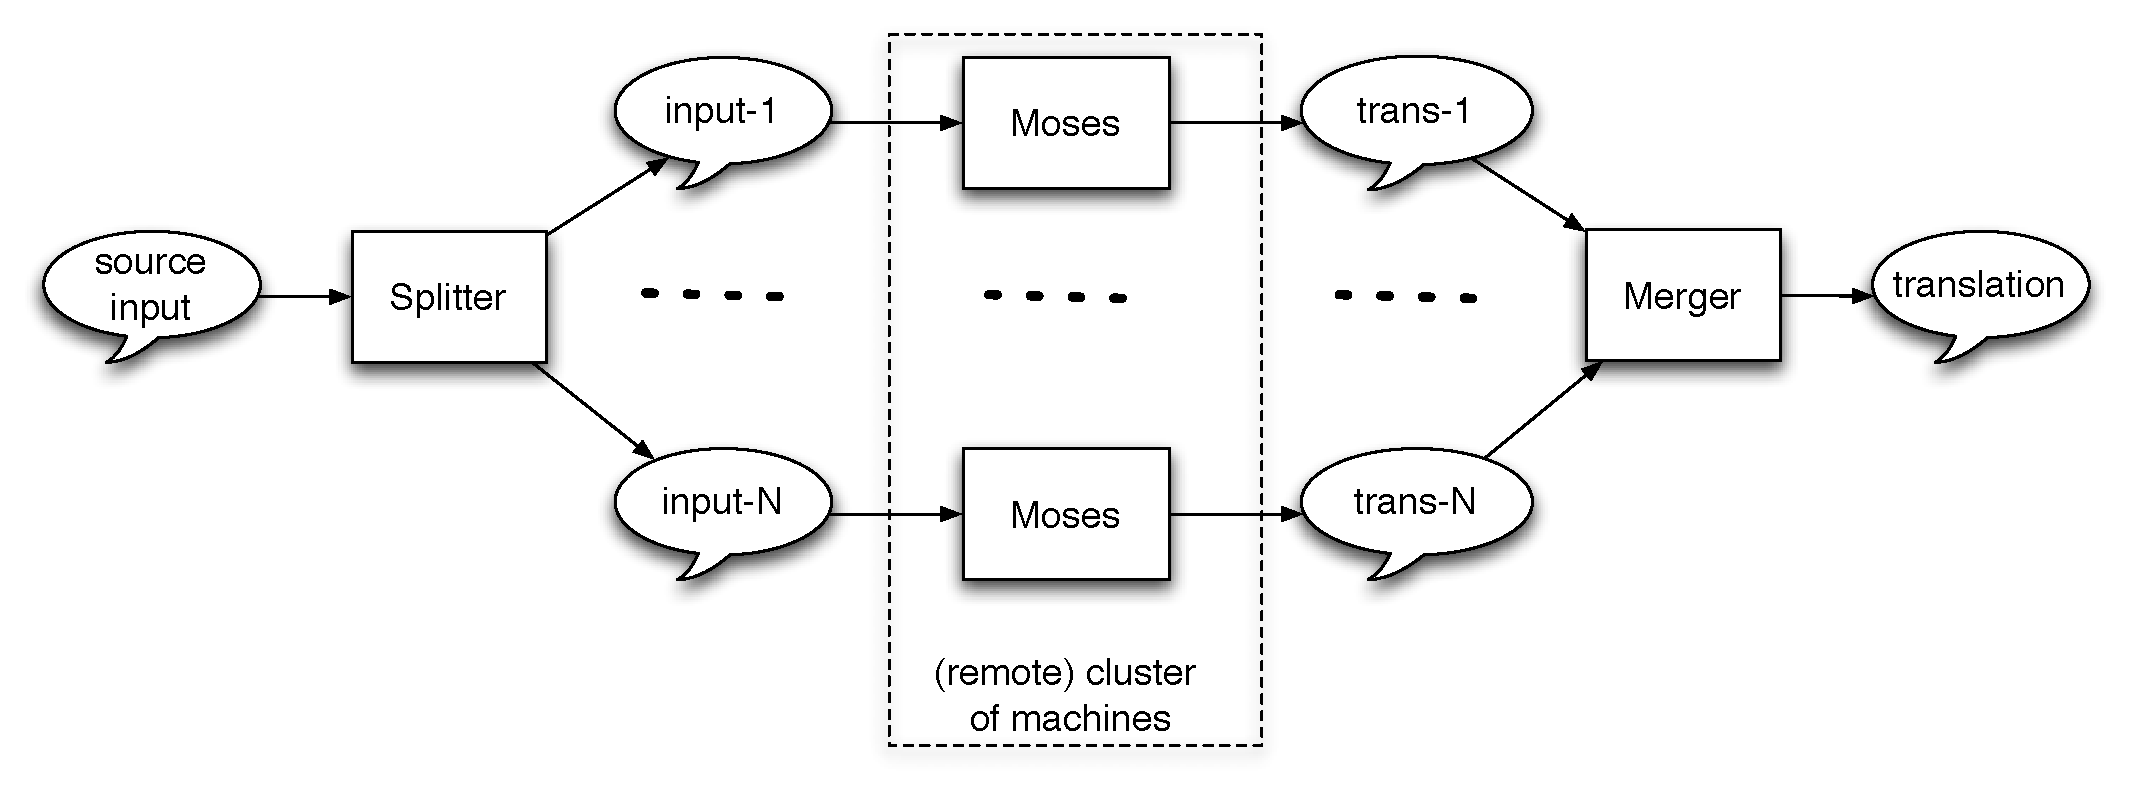
\includegraphics[width=\columnwidth]{Moses-parallel}
\caption{The parallelization module for {\tt Moses}.}
\label{fig:parallel}
\end{center}
 \end{figure}
 
As shown in Figure~\ref{fig:parallel}, the procedure we implemented is reasonably easy:
first, the source input is equally divided into $N$ parts, then $N$ instances of the {\tt Moses} translate them; finally, the full translation is obtained by ordering and merging the translation of all input parts.

All {\tt Moses} instances are assumed to run on a (possibly remote) cluster. No restriction on the number of {\tt Moses} instances is given.


Time to perform a full translation with one {\tt Moses} instance comprises the time to load data, which is constant, and time to translate the input, which is proportional to its size.
The parallelization module requires an additional time to access the cluster, which is strictly related to the real load of the cluster itself and hardly forecastable.
Time to split the input and merge the output can be considered negligible with respect to the translation time.
Moreover, an "ending" delay can be observed because the merging module should wait that all decoders have completed their translations, and this does not necessarily happen at the same time. A good splitting policy which allows a balanced translation time among all decoders,  improves the effciency of the whole parallelization module.

We tested the gain in time that  the parallelization module can provide to the toolkit on the Spanish-English EuroParl task. 3 input sets were created of 10, 100 1000 sentences and translated using a standalone  {\tt Moses}, and the parallelization module exploiting difference number of {\tt Moses} instances (1, 5, 10, 20).
Decoders ran on the 18-processor CLSP cluster. As in the real situation, its load was not in control, and hence the immediate availability of the processors was not assured. Table~\ref{tbl:parallel-time} reports the average translation times for all conditions.

Some considerations can be drawn by inspecting these figures.
\begin{itemize}
\item Parallelization is not effective if source input is small, because time to access the cluster dominates overall runtime.
\item Trivially, there is no reason to use the parallelization module if just one processor is required. 
\item Parallelization is beneficial if more instances of {\tt Moses} are exploited.
\item The gain in time is not exactly proportional to the number of decoder instances, mainly due to the effect  of ``ending" delay, where results are aggregated .
\end{itemize}


\begin{table}
\label{tbl:parallel-time}
\begin{center}
\begin{tabular}{r|rrrrr}
                 & standalone   &1 proc  & 5 proc  &  10 proc   &  20 proc\\
                 \hline
     10 sentences   &  6.3  &  13.1 &  9.0  &  9.0   &     --  \\
  100 sentences   &  5.2  &  5.6    &  3.0  &  1.7   &   1.7 \\
1000 sentences   & 6.3   &  6.5    &  2.0  &  1.6   &   1.1 \\
\end{tabular}
\caption{Average time (seconds) to translate 3 input sets with a standalone {\tt Moses} and with its parallel version.}
\end{center}
\end{table}

In conclusion, the choice of the number of splits $N$ is essential for a good efficiency of the parallelization module, and depends on the available computational power, the cluster load, and the average translation time of the standalone decoder.



\section{Tuning}
\label{merttuning}
%{\sc Nicola Bertoldi}
\newcommand{\e}{{\bf e}}
\newcommand{\f}{{\bf f}}
\label{sec:tuning}
As described in Section~\ref{sec:slt}, {\tt Moses} decoder relies on a log-linear model to search for the best translation $\e^*$ given an input string $\f$:
\begin{equation}
\e^* = \arg\max_{\e}  \Pr(\e \mid \f) =\arg\max_{\e}  p_{\lambda}(\e \mid \f) = \arg\max_{\e} \sum_i \lambda_i h_i(\e,\f)
\end{equation}

Main components of a  log-linear model are the real-valued feature functions $h_i$ and their real-valued weights $\lambda_i$. To get the best performance from this model all components need to be estimated and optimized for the specific task the model is applied to.

Feature functions model specific aspects of the translation process, like the fluency, the adequacy, the reordering. Features can correspond to any function of $\e$ and $\f$, and  there is no restriction about the values they assume.
Some features are  based on statistical models which are estimated on specific training data.

Feature weights are useful to balance the (possibly very different) ranges of the feature functions, and to weigh their relative contribution. The most common way to estimate the weights of a log-linear model is called Minimum Error Rate Training (MERT). It consists in an automatic procedure which search for the weights minimizing translation errors on a development set.

In this section we assume that the input type is text string, but trivially there is no matter if input is a Confusion Network, because MERT just estimates weights of the log-linear combination regardless the type and the number of features.


Let $\f$ be a source sentence and ${\bf ref}$ the set of its reference translations; 
let $\bf Err(\e;ref)$ be an error function which measures the quality of a given translation $\e$ with respect to the references ${\bf ref}$. The MERT paradigm can be formally stated as follows:

\begin{eqnarray}
\e^*= \e^*(\lambda) = \arg\max_{\e}  p_{\lambda}(\e \mid \f) \\
\bf \lambda^* = \arg\min_{\lambda} {\bf Err} (\e^*(\lambda);ref)
\label{eq:directMT}
\end{eqnarray}
where $\e^*(\lambda)$ is the best translation found by the decoder exploiting a given set of weights $\lambda$.

The error function needs to be computed automatically from $\e$ and ${\bf ref}$ without human intervention. Word Error Rate (WER), Position Independent Word Error Rate (PER), (100-BLEU score), NIST score, or any combination of them are good candidates as automatic scoring functions.

An error function is rarely mathematically sound, and hence an exact solution of the previous problem is not usually known. Hence, algorithms like the gradient descent or the downhill simplex, are exploited which iteratively approximate the optimal solution. Unfortunately, these approximate algorithms frequently get stuck in a local optimum.

\begin{figure}
\begin{center}
 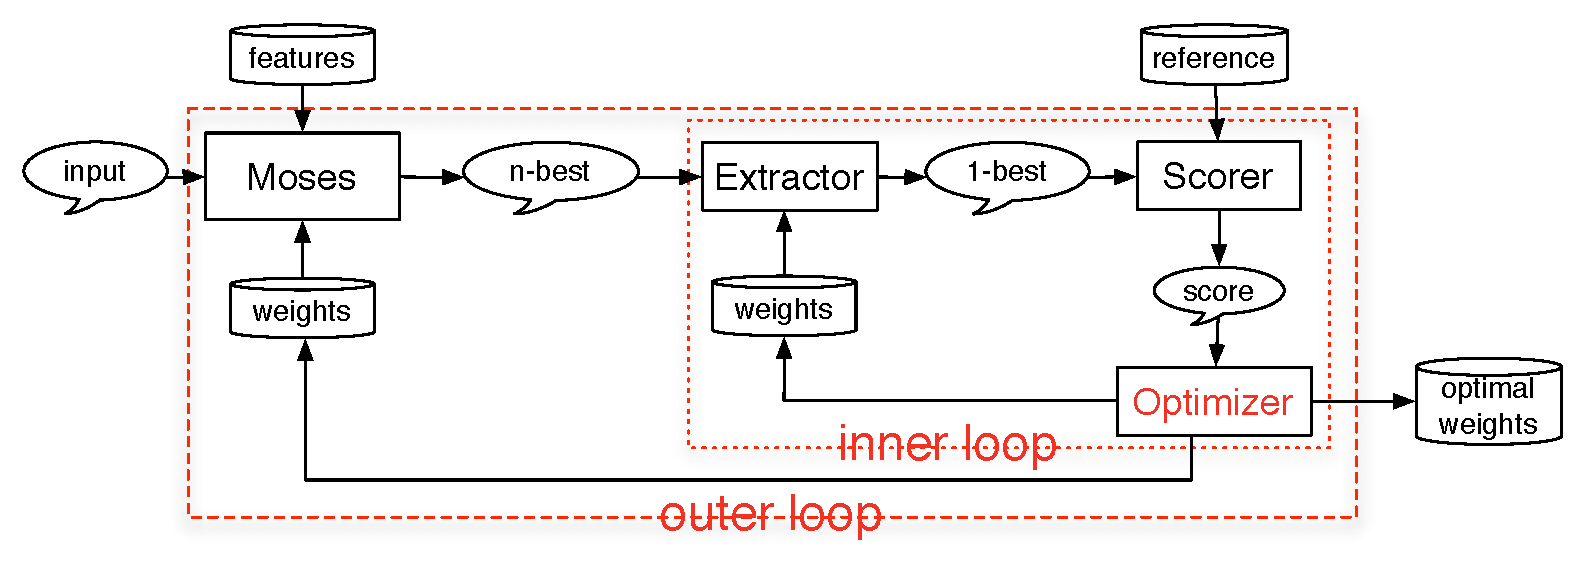
\includegraphics[width=\columnwidth]{MER-ext}
\caption{An high-level picture of the Minimum Error Rate Training module for the optimization of the feature weights.}
\label{fig:MERT}
\end{center}
 \end{figure}
 
The MERT procedure we implemented during the workshop is depicted in Figure~\ref{fig:MERT}. 
It is based on two nested loops, which are now described.

In the outer loop 
\begin{enumerate}
\item initial weights $\lambda^0$, an empty list of translation hypotheses $T^0$, and the iteration index $t=0$ are set;
\item {\tt Moses} translates the input with  $\lambda^t$ and generates a list of $N$-best translation hypotheses $T^t$;
\item $T^t$ are added to the previous lists $T^0, \ldots T^{t-1}$;
\item the inner loop is performed (see below) on the new list $\bigcup_{i=0}^{t}T^i$ and with the weights $\lambda^t$;
\item the  new set of weights $\lambda^{t+1}$ provided by the inner loop are set;
\item t is increased by 1, and the loop restarts from 2.
\end{enumerate}
The outer loop ends when the list of translation hypotheses does not increase anymore.

In the inner loop which  is fed with a list of hypotheses and a set of weights $\bar \lambda$
\begin{enumerate}
\item initial weights $\lambda^0$ are set to $\bar \lambda$, and the iteration index $s=0$ is set;
\item all translation hypotheses in the list are rescored according with the actual weights $\lambda^s$
and the best-scored hypothesis is extracted ({\tt Extractor});
\item the error measure of such translation is computed ({\tt Scorer});
\item the {\tt Optimizer} suggests a new set of weights $\lambda^{s+1}$;
\item $s$ is increased by 1, and the loop restarts from 2.
\end{enumerate}
The inner loop ends when the error measure does not improve anymore.
As the {\tt Optimizer} provides a local optimum for the weights, and strongly depends on the starting point $\bar \lambda$, the inner loop starts over several  times with different choices of $\bar \lambda$. The first time the weights $\lambda^t$ used by {\tt Moses} in the last outer loop are applied; the next times random sets are exploited. The best set of weights are then provided to the outer loop again.

Instead of standard approximate algorithms like the gradient descent or the downhill simplex, in the workshop we employed an {\tt Optimizer} based on the idea proposed by \cite{Och2003c} and developed by David Chiang (USC-ISI). The algorithm strongly relies on the availability of a finite list of translation alternatives, because this allows a discretization of the $r$-dimensional space of the weights ($r$ is the number of weights). This makes the search of the optimum  faster. The algorithm iteratively optimizes one weight at a time.

The {\tt Scorer} employed in the workshop computes BLEU score.

The time spent for each iteration of the outer is basically proportional to the size of the input  because the translation of the whole input is required. The time for each iteration of the inner loop is proportional to the amount of translation hypotheses because all of them have to be re-scored and evaluated,




\subsection{Tuning Experiments}\label{sec:exp-tuning}

We analized how much the experimental set up affects the effectiveness of MERT. In particular, the amount of translation hypotheses extracted in each outer loop and the size of the development set are taken into account.

Experiments were carried out on two tasks, namely the translation of proceedings of 
the European Parliament from German into English, and the translation  of  speeches from the  European Parliament Plenary Sessions (EPPS) from Spanish to English.

\paragraph{The German-English EuroParl task}
\label{sec:ge-en-europarl-task}
EuroParl \cite{koe:05} is a collection of parallel text in 11 languages from the proceedings of the European Parliament. We worked on the German-English language pair. Training data consist of 751 K sentence pairs. 2000 sentences are provided both for parameter tuning and for testing.  Statistics about training data, development and test sets are reported in Table~\ref{tbl:ge-en-europarl-data}
Sentences in the development and test sets are provided with just 1 reference translation each.  

\begin{table}[th]
\begin{center}
\begin{tabular}{lrr|rr|rrr}
        &  \multicolumn{2}{c|}{Train}   &  \multicolumn{2}{c|}{Dev}    &  \multicolumn{2}{c}{Test}\\
 \hline
        &  Ger   &   Eng  &  Ger   &   Eng  &  Ger   &   Eng     \\
 \hline
Sentences    & \multicolumn{2}{c|}{751 K} & \multicolumn{2}{c|}{2,000} & \multicolumn{2}{c}{2,000}\\
Words & 15 M & 16 M & 55,136 & 58,652 & 54,247 & 57,945\\
Vocabulary  & 195 K & 66 K & 8,796 & 6,114& 8,668 & 6,054&\\
Phrase Pairs  & \multicolumn{2}{c|}{12 M}\\
Phrases & 9 M & 8 M \\
\end{tabular}
\caption{Statistics of the German-English EuroParl task. Word counts of  English dev and test sets refer
 the first reference translation. }
\label{tbl:ge-en-europarl-data}
\end{center}
\end{table}

Models employed in the decoder were estimated with the {\tt Moses} toolkit. A 3-gram target language model was used.

\paragraph{The EPPS task}
\label{sec:epps-task}
The EPPS task consists in translating speeches from the  European Parliament  from Spanish to English, This task was organized in the TC-STAR 2005\footnote{http://www.tc-star.org} Evaluation Campaign. 

Speeches included in the development and test sets are automatically recognized by LIMSI, France, which kindly provided the word lattices, and Confusion Networks were extracted from them using the {\tt lattice-tool} software of the {\tt SRILM Toolkit} \cite{stolcke:02}. Instead, training data for the EPPS task consists of the Final Text Editions of the speeches, which are significantly human-revised versions of the simultaneous transcriptions.
Statistics about the training, development and testing  data are reported in Table~\ref{tbl:epps-data}.  
Sentences in the development and test sets are provided with two reference translations each.  


\begin{table}[th]
\begin{center}
\begin{tabular}{lrr|rr|rrr}
        &  \multicolumn{2}{c|}{Train}   &  \multicolumn{2}{c|}{Dev}    &  \multicolumn{2}{c}{Test}\\
 \hline
        &  Spa   &   Eng  &  Spa   &   Eng  &  Spa   &   Eng     \\
 \hline
Sentences    &   \multicolumn{2}{c|}{1,308 K} & \multicolumn{2}{c|}{2,643} & \multicolumn{2}{c}{1,073}\\
Words & 37 M & 36 M & 20,384 & 20,579 & 18,890 & 18,758\\
Vocabulary   & 143 K & 110 K & 2,883 &  2,362  & 3,139 & 2,567 \\
Phrase Pairs   & \multicolumn{2}{c|}{83 M}\\
Phrases   & 48 M & 44 M\\
\end{tabular}
\caption{Statistics of the EPPS speech translation task. Word counts of  dev and test sets sets refer
to human transcriptions (Spanish) and the first reference translation (English). }
\label{tbl:epps-data}
\end{center}
\end{table}

Models were estimated with the {\tt Moses} training tools, apart from the 4-gram target LM which was trained with the IRST LM Toolkit on 47 M running words.


\paragraph{MERT vs. amount of translation alternatives}
First, we tested whether and how the amount of translation alternatives generated by {\tt Moses} impacts on the tuning. For this experiment the EuroParl task was selected. Several MERTs were performed constraining {\tt Moses} to generate a different number of translations in each outer loop ($N=100, 200, 400, 800$). The sets of weights obtained after each iteration of the outer loop are then used to translate the test set. Figure~\ref{fig:MERT-epps-nbest} shows the achieved BLEU score in the different conditions.

\begin{figure}[ht]
\begin{center}
\label{fig:MERT-epps-nbest}
 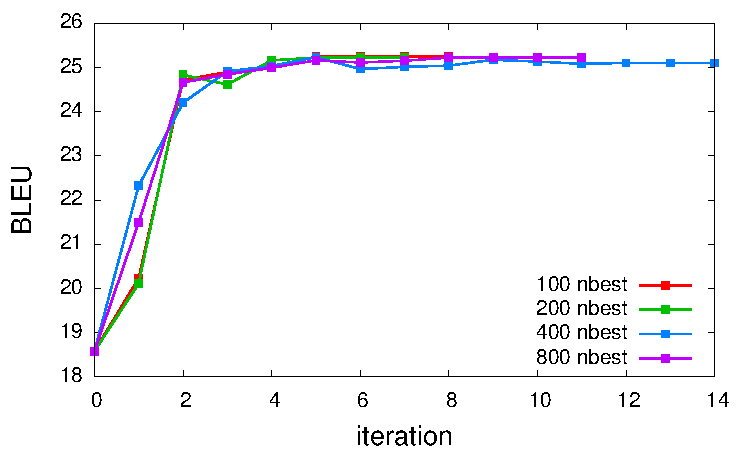
\includegraphics[width=0.75\columnwidth]{MERT-nbest}
\caption{Performance (BLEU score) achieved on the EuroParl test set using feature weights optimized exploiting an increasing number of translation alternatives of the development set.}
\end{center}
 \end{figure}

We observe that convergence is reached after few iterations (5-6). This fact is positive because it allows to run {\tt Moses} only few times.

The weights obtained in the first iterations seem to award the use large $N$, but this effects vanishes very soon because the set of translation alternatives is continuously enlarged.

The final sets of weights perform very similar for each experimental condition; this is also positive because a limited number of $N$-best can be extracted, speeding up both the translation process and the inner loop.


\paragraph{MERT vs. amount of translation alternatives}
We also tested the impact of the size of the development set on the MERT procedure in both EuroParl and EPPS tasks. 
From the  development set of the EuroParl we extracted 4 subsets of 100, 200 400 and 800 sentences, respectively. 529 sentences are randomly selected from the EPPS development set .
The sets of weights obtained after each iteration of the outer loop are then used to translate the corresponding test sets.

\begin{figure}
\begin{center}
\label{fig:MERT-europarl-devsize}
 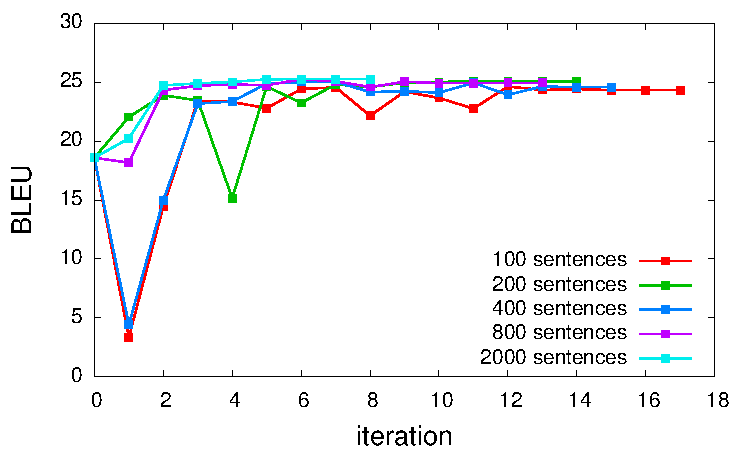
\includegraphics[width=0.75\columnwidth]{europarl-devsize}
\caption{Performance (BLEU score) achieved on the EuroParl test set using feature weights optimized on  development sets of increasing size.}
\end{center}
 \end{figure}


\begin{figure}
\begin{center}
\label{fig:MERT-epps-devsize}
 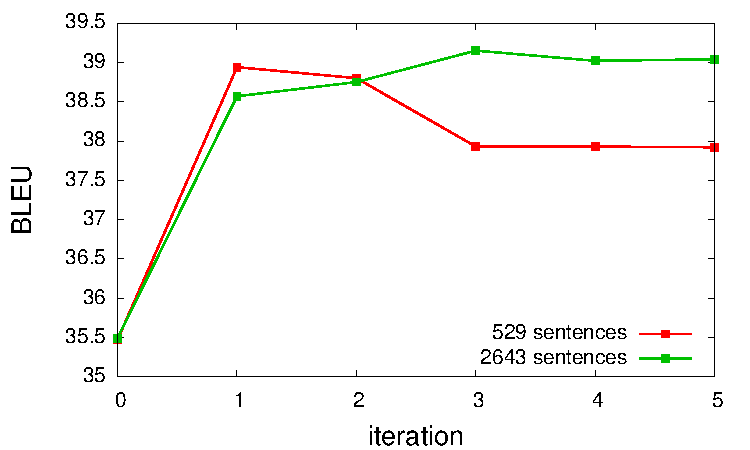
\includegraphics[width=0.75\columnwidth]{epps-cn-devsize}
\caption{Performance (BLEU score) achieved on the EPPS test set using feature weights optimized on  development sets of increasing size.}
\end{center}
 \end{figure}

Figures~\ref{fig:MERT-europarl-devsize} and \ref{fig:MERT-epps-devsize} show the achieved BLEU score in the different conditions for the EuroParl and EPPS tasks, respectively.  Plots reveal that more stable and better results are obtained with weights optimized on larger dev set; moreover, EuroParl experiments show that MERT with larger dev set tends to end in less iterations.
In general, these experiments show that 2 iterations give the biggest relative  improvement and that next iterations, which slightly improve on the dev set, are risky on the test set.

This behavior is explained by the tendency of MERT procedure to overfit the development data. Possible ways to limit the overfitting problems consists in enlarging the dev set  and ending the tuning after few iterations.
The former solution increases the time of tuning, while the latter make it faster and more robust. with respect to differences between dev and test sets. It is also trivial to stress that the development  data should be as close as possible to the test domain.


\paragraph{Comparison of different optimization algorithm} We also compared our optimization algorithm against the downhill simplex algorithm. For this experiment we employed {\tt Moses} in the EPPS task.

Table~\ref{tbl:MERT-epps-algorithm} reports the increment of BLEU score achieved on the development and test sets after MERT; it shows that our approach is definitively competitive with (and slightly better than) the widely-used downhill simplex algorithm. The number of iterations to converge are similar, too.
Moreover, the improvements achieved on the dev and test sets are comparable.


 \begin{table}[ht]
\begin{center}
\label{tbl:MERT-epps-algorithm}
\begin{tabular}{l|ccc}
algorithm               & iteration & \multicolumn{2}{c}{$\Delta$ BLEU}\\
                                &                & dev & test\\
\hline
CLSP-WS              & 6 & +3.2 & +3.6 \\
downhill simplex  & 7 & +2.9  & +3.4\\
\end{tabular}
\caption{Performance improvement (absolute BLEU score) achieved on the EPPS task using two different optimization algorithm.}
\end{center}
\end{table}

\paragraph{MERT vs. different input types} Finally, we performed two separate MERT for the two input types handled by {\tt Moses}, namely text and Confusion Networks. The human transcriptions ({\tt verbatim}) and the CNs of the development data of the EPPS task were exploited. Weights optimized in the {\tt verbatim} condition were applied to translate both human transcriptions ({\tt verbatim}), the best automatic transcriptions ({\tt 1-best}),  and the consensus decoding transcriptions ({\tt 1-best-CN}) extracted from the CNs \cite{mangu:00} by taking the most probable words of  each column. Weights optimized in the {\tt CN} condition were applied to the CNs of the test set.
The increments achieved on the development and test data are reported in Table~\ref{tbl:MERT-epps-summary}.


 \begin{table}[ht]
\begin{center}
\label{tbl:MERT-epps-summary}
\begin{tabular}{l|cc}
input                    &\multicolumn{2}{c}{$\Delta$ BLEU}\\
                             & dev & test\\
\hline
{\tt verbatim}  &  +1.9 & +2.1\\
{\tt 1best}        &  +2.1 & +2.2\\
{\tt 1best-CN} &  +1.6 & +2.2\\
\hline
{\tt CN}            &  +3.2 & +3.6\\
\end{tabular}
\caption{Performance improvement  (absolute BLEU score) achieved on the EPPS task using different input types.}
\end{center}
\end{table}

We observe that improvement on the test set ranges from 2.1 to 3.6 absolute BLEU points, and that it is consistent between dev and test. The bigger increase for the CNs is probably due to a choice of the initial set of weights performing worse than the corresponding set for the {\tt verbatim} condition.






\section{Efficient Language Model Handling}
%{\sc Marcello Federico}

In this section we review main concepts related to the handling of language models (LMs) 
at run time, that is during the decoding phase. Concerning the estimation of language 
models the reader can refer to the documentation of publicly available tools, such as 
SRI LM Toolkit and the CMU-Cambridge SLM toolkit.  These toolkits, in general, provide many 
methods for estimating n-gram probabilities and are capable of generating  a static 
representation of an n-gram LM, a text or binary file, that can  be used within other programs.   

The motivation of developing software for handling LMs at run time is that efficiency, both 
in time and space, can be gained by exploiting peculiarities  of the way they are used by the 
hosting program, namely the decoder.  

The need for efficient LM handling comes from the  intrinsic data-sparseness of language corpora. 
Empirically, for a given size of n-grams,   the set of
observations increases  almost linearly with the size  of the training
data.  Hence, the trend of using larger and larger training corpora compels for careful memory
usage.

In general, to efficiently  store observations and probabilities in a
computer  memory the  following approaches  can be  tackled:  pruning  rare or unreliable observations, designing compact data-structures,  and applying data compression. While the observation pruning is typically embedded in the tools to estimate the LMs, we focused
on the other aspects, which are more related to the way the LM is used by a specific program.

In the following we discuss some of the features of our implementation: the representation of 
n-gram LMs, the quantization of probabilities, and  the use of cache memories. 

\subsection{LM representation}
In our implementation N-gram are stored in a data structure which indeed privileges memory
saving rather than access time.  In particular, single components of each n-grams are accessed 
via binary search and stored with 3 bytes, probabilities and back-off weights are instead stored
in 4 bytes, namely  floating point numbers. Improvements in memory savings are obtained by 
quantizing both back-off weights and probabilities. 

\begin{figure}
\begin{center}
 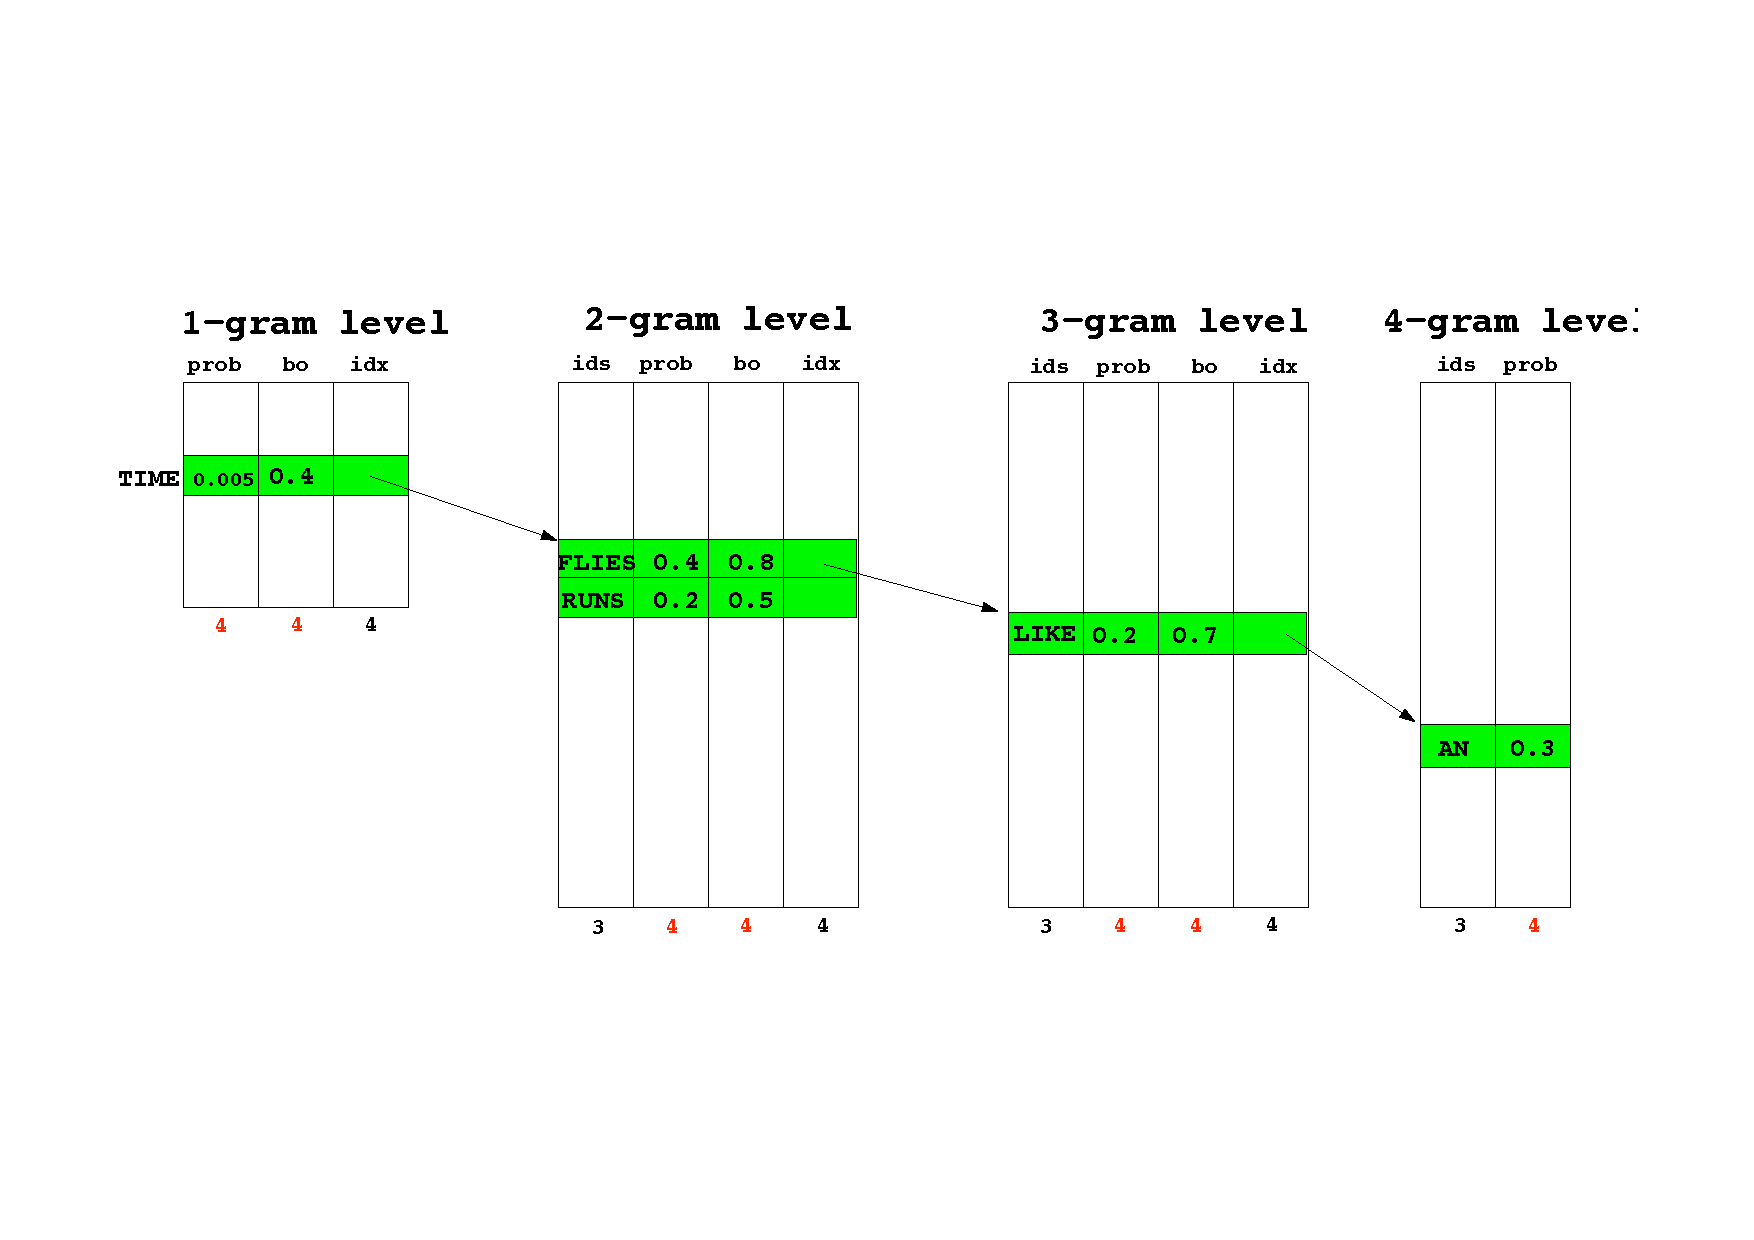
\includegraphics[width=\columnwidth]{marcello-lmstruct}
\vspace{-3cm}
\caption{Data structure for storing n-gram language models.}
\label{fig:LM-struct}
\end{center}
 \end{figure}


\subsection{Probability quantization}

Quantization provides an effective way of reducing the number of bits
needed to store floating point variables. The quantization process
consists in partitioning the real space into a finite set of $k$ {\em
quantization levels} and identifying a center $c_i$ for each level,
$i=1,\ldots, k$. A function $q(x)$ maps any real-valued point $x$ onto
its unique center $c_i$.  Cost of quantization is the approximation
error between $x$ and $c_i$. 

Previous  experiments (cite ) suggested us to apply the so-called
binning method.  The binning method partitions data points into uniformly
populated intervals or {\bold bins}. The center of each bin corresponds
to the mean value of all points falling into it.  If $N_i$ is the
number of points of the $i$-th bin, and $x_i$ the smallest point in
the $i$-th bin, a partition $[x_i,x_{i+1}]$ results such that $N_i$ is
constant for each $i=0,\ldots, k-1$, where $x_k=1$ by default.
The following map is thus defined:
$$q(x)=c_i \mbox{ if } x_i<=x<x_{i+1}.$$

In particular, our implementation uses the following {\bold greedy} strategy: bins are
build by uniformly partition all different points of the data set.  Finally, quantization is 
applied separately at each n-gram level and for each kind of score, that is probabilities
or back-off weights.  The level of quantization is set to 8 bits, that experimentally showed 
to cause  no measurable loss in performance.

Quantization can be applied on any LM represented with the ARPA format. Quantized LMs
can be converted into a binary format that can be efficiently uploaded at decoding time.


\subsection{Caching of probabilities}

In order to overcome limitations of access time, caching is applied. The potential advantage
of caching during MT decoding is made evident by the plot in Figure~\ref{fig:LM-calls}. 
It shows all calls of 3-gram probabilities by the search algorithm during the decoding of
the following German sentence:

{\bold ich bin kein christdemokrat und glaube daher nicht an wunder . doch ich m\"ochte dem europ\"aischen parlament , so wie es gegenw\"urtig beschaffen ist , f\"ur seinen grossen beitrag zu diesen arbeiten danken.}

During decoding of the sentence, about 120,000 different 3-grams are called for a total 
of about  1.7 million times.  The fact that a relatively small subset of 3-grams is frequently
accessed for each sentence suggest to store all of them into a cache. Each time a new 
sentence is decoded, the cache is reset and n-gram probabilities are added as soon as they are 
needed.  Additional caches are also used to store LM states, and all partial  n-grams 
searched in the data in order to limit the number of binary searches performed.

\begin{figure}
\begin{center}
 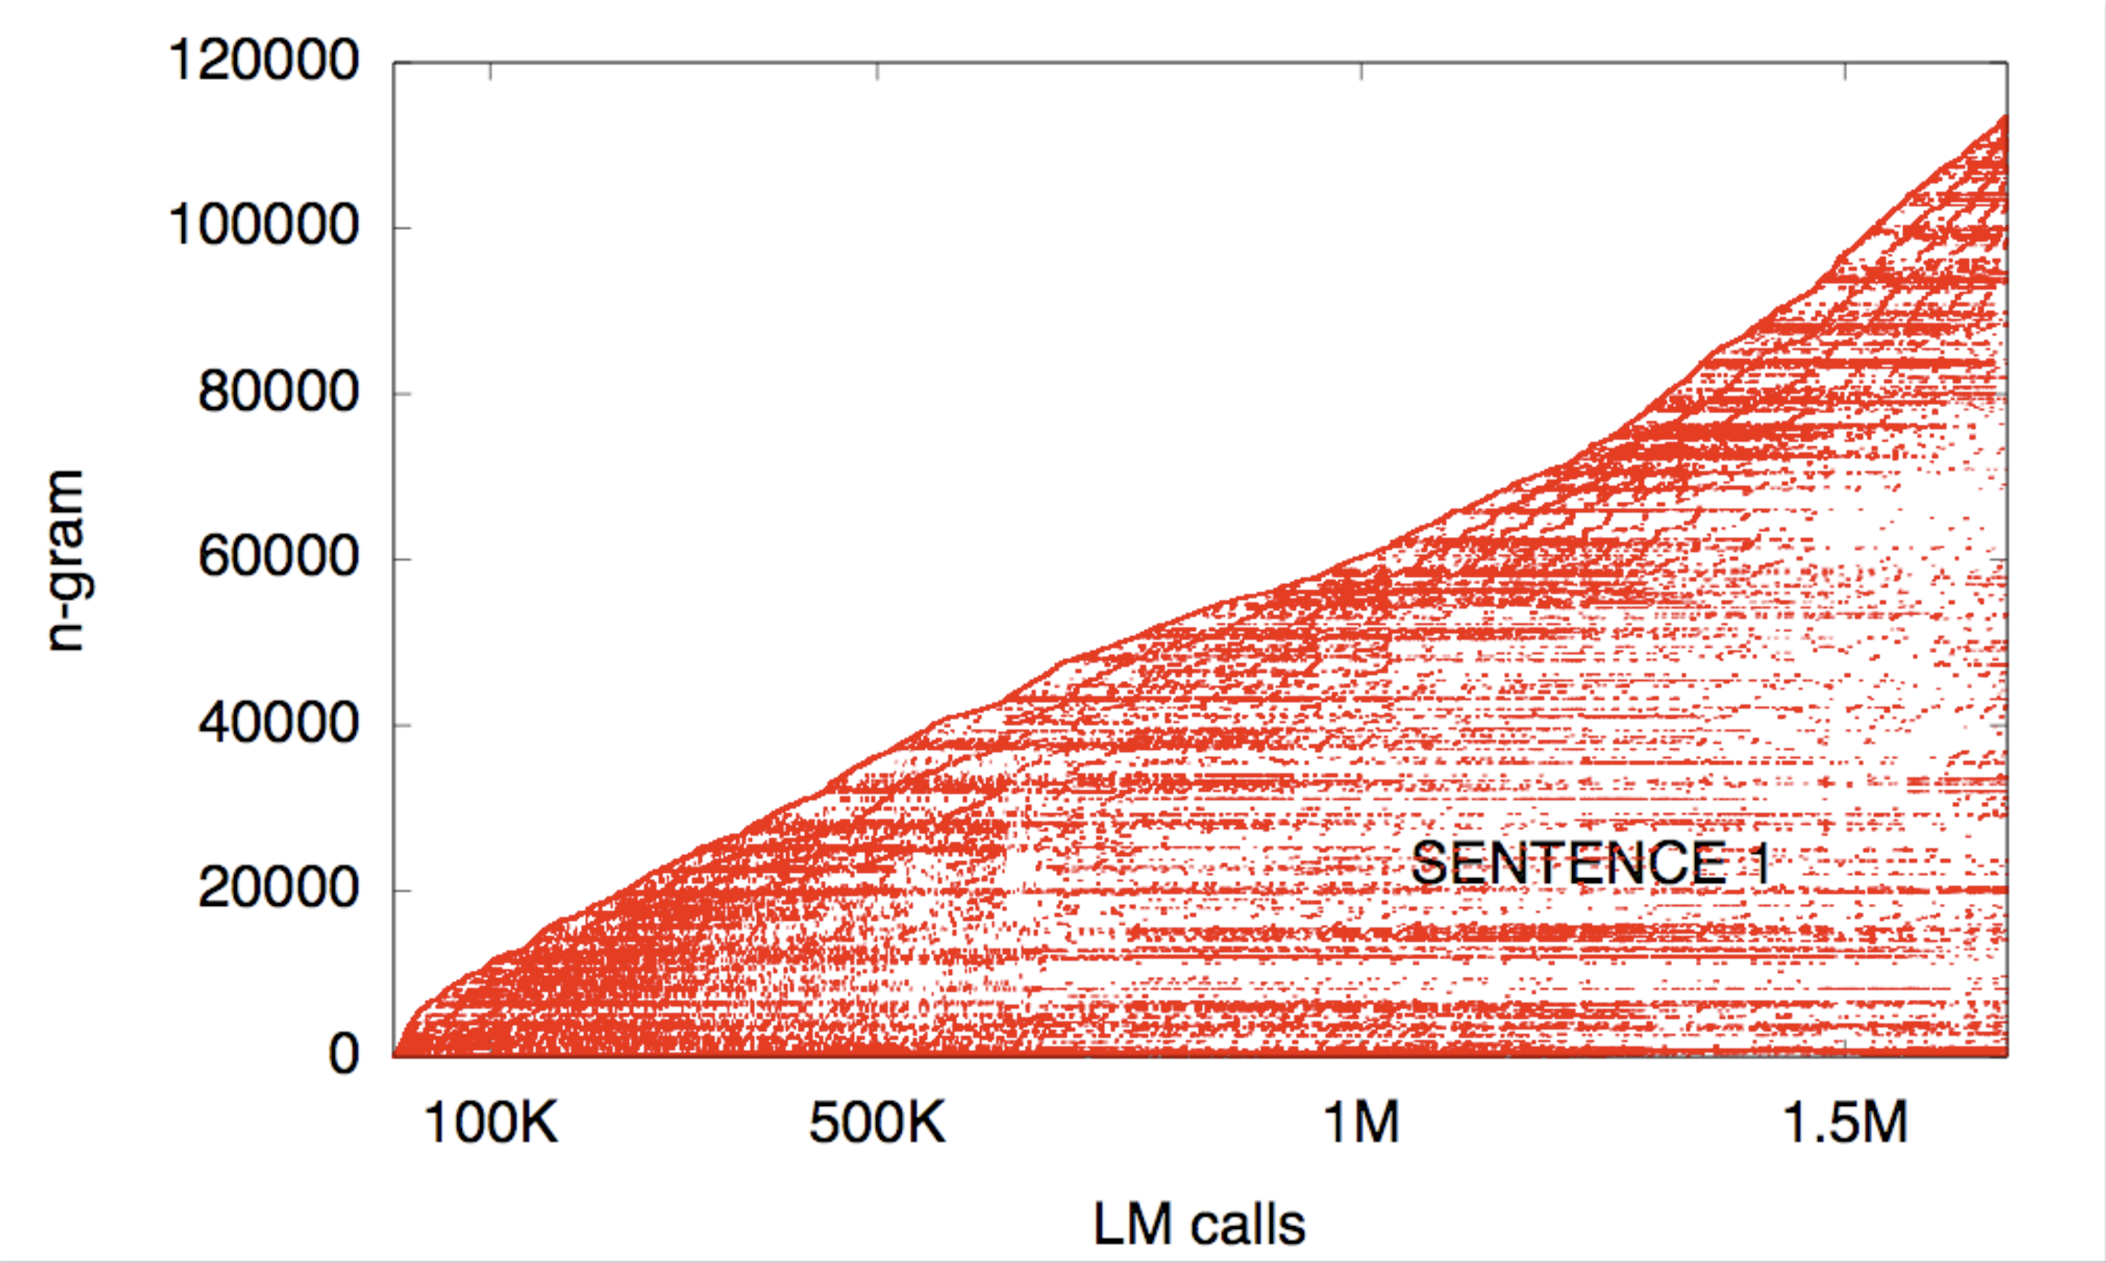
\includegraphics[width=\columnwidth]{marcello-lmcalls}
\caption{LM calls during decoding of a sentence by Moses.}
\label{fig:LM-calls}
\end{center}
 \end{figure}
 
\chapter{Conclusions}
The 2006 JHU Summer Workshop on statistical machine translation brought together efforts to build an open source toolkit and carry out research along two research goals: factored translation models and confusion network decoding.

We are optimistic that the toolkit will be the basis of much future research to improve statistical machine translation. Already during the workshop we received requests for Moses, and at the time of this writing the Moses web site\footnote{\tt http://www.statmt.org/moses/} attracts 1000 visitors a month and a support mailing list gets a few emails a day. The performance of the system has been demonstrated, included by newcomers who took the software and obtained competitive performance at recent evaluation campaigns.

Our work of factored translation models has been demonstration not only in the experiments reported in this report, but also in follow-up work at our home instititions and beyond, resulting in publications in forthcoming conferences and workshops.

Our work on confusion network decoding has been demonstrated to be helpful to integrate speech recognition and machine translation, and even in more recent follow-up work, the integration of ambiguous morphological analysis tools to better deal with morphological rich languages.

While six weeks in summer in Baltimore seem like a short period of time, it was a focal point of many of our efforts and resulted in stimulating exchange of ideas and the establishment of lasting research relationships.

\bibliographystyle{apalike}
\bibliography{biblio}

\printindex


\appendix


\chapter{Follow-Up Research Proposal\\
A Syntax and Factor Based Model for Statistical Machine Translation}

\newcommand{\gen}{\hbox{GEN}}
\newcommand{\rep}{\bar{\phi}}
\newcommand{\Rep}{{\Phi}}
\newfont{\msym}{msbm10}
\newcommand{\reals}{\mbox{\msym R}}
\newcommand{\pav}{\bar{\alpha}}
\newcommand{\ip}[2]{{#1} \cdot {#2}}
\def\parcite#1{(\cite{#1})}
\def\perscite#1{\cite{#1}} % works like acl-style \newcite

This appendix contains Brooke Cowan's  proposal for follow-on research, which was selected for additional funding by the National Science Foundation.   

\section{Introduction}
\label{intro}

This year's Summer Workshop on Language Engineering at Johns Hopkins
University focused in part on the development of an open source
toolkit for statistical machine translation
(SMT). The
toolkit's decoder, known as {\bold Moses}, replicates the functionality
exhibited by the phrase-based decoder Pharaoh \parcite{koe:04}. One of
the weaknesses of traditional phrase-based models is their inability
to incorporate syntactic information in a direct and overt manner. For
instance, most English sentences contain a subject and a verb, but
there is no straightforward way to model this fact within the
phrase-based framework. Furthermore, there are translation
correspondences that are simple to describe using part-of-speech
information but difficult to model using lexical items
alone. (E.g., a French noun phrases that has the
part-of-speech sequence {\bold determiner noun adjective} will most
likely in English be {\bold determiner adjective noun}.)  Moses addresses
the latter problem by extending the phrase-based framework to include
{\bold factors}; hence, it exemplifies a {\bold factor-based approach} to
statistical machine translation. Factor-based models behave much like
phrase-based models, but have the additional capability to take into
account information such as morphology and parts of speech, lemmas,
and phrase bracketing in the source and/or target languages during
decoding.

The experimental results from this summer's workshop indicate that
using factors can indeed improve translation performance. However,
observation of Moses' translation output indicates that, even when
BLEU scores improves, the system often does not adhere to basic global
syntactic constraints\footnote{We use the word {\bold global} here to
refer to properties that require examination of the clause in its
entirety, such as {\bold a clause will usually contain a finite verb}
and {\bold a clause will never have more than one finite verb}.} of the
target language. We propose to address this problem by using a
syntax-based system that explicitly models syntactic constraints in
conjunction with the factor-based system developed this summer. A
baseline version of the syntax-based system has been implemented at
the Laboratory for Computer Science and Artificial Intelligence
(CSAIL) at MIT \parcite{cow:06}. A fundamental component of this system
is a discriminatively-trained model that takes as input a
source-language parse tree and produces a detailed target-language
syntactic structure called an {\bold aligned extended projection}, or
AEP. AEPs may include information such as the main verb of the output
sentence, the number and type of its arguments, and the correspondence
(alignment) between source-side and target-side modifiers. The
discriminative AEP model provides an extremely flexible framework for
experimentation with a variety of language pairs and treebanking
styles. Most importantly, it provides a framework for modeling global
sytactic constraints of both the target language, as well as syntactic
correspondences between the source and target language.

This proposal is structured as follows: we continue this section with
some background on phrase-based and factor-based approaches to SMT; in
Section~\ref{framework}, we describe the syntax-based model in more
detail; and in Section~\ref{future}, we outline the work that we
propose to carry out this year to integrate the syntax-based and the
factor-based models.

\subsection{From Phrase-Based to Factor-Based Translation}
Phrase-based systems (e.g., \parcite{koe:04,koe:03,Och2002,ochney:00})
advanced the state-of-the-art in statistical machine translation
during the early part of this decade. They surpassed the performance
of earlier models, proposed by researchers at IBM and known as the
{\bold IBM models} \parcite{Brown1993}, which used alignments between words
(predicted using the EM algorithm) to estimate the values of
translation parameters in a generative model.  Phrase-based models
combine the word alignments induced by the earlier SMT models to
produce alignments between substrings of source and target text,
which, in these models, are called {\bold phrases}.\footnote{Note that
these phrases do not have to be phrases in any linguistic sense.}
These phrasal translations, together with a search algorithm that
looks for a high-scoring solution, form the basis of the phrase-based
framework.

The current state-of-the-art phrase-based systems are log-linear
models of the conditional probability of the target ($e$) given the
source ($f$):

\begin{equation}
Pr(e|f) = \frac{\exp{\sum_{i} \lambda_i h_i(e,f)}}{\sum_{e'} \exp{\sum_{i} \lambda_i h_i(e',f)}}
\label{loglinear}
\end{equation}


The $\lambda_i$ are weights on feature functions $h_i(e,f)$. The
weights are usually trained using minimum error rate training
\parcite{Och2003c}, although recently an online perceptron training
algorithm has also been shown effective \parcite{lia:06}. There are
usually on the order of ten feature functions, among which may be

\begin{itemize}
\item bidirectional phrase models (models that score phrasal translations);
\item bidirectional lexical models (models that consider the
appearance of entries from a conventional translation lexicon in the
phrasal translation);
\item $n$-gram target-language models ($n$-th order Markov models
whose parameters are trained on large amounts of monolingual data; the
probability of each word in a phrase is conditioned on the preceding
$n-1$ words, and the probability of the phrase is the product of the
probabilities the words);
\item distortion models (models that consider how source phrases get
reordered in the translation).
\end{itemize}

Phrase-based models address a severe limitation of the early
word-based models, which are restricted to many-to-one mappings
between source and target words. This means that if the Spanish phrase
{\bold el libro del ni\~{n}o} were translated as {\bold the boy's book} in
the data, the pairing between {\bold el libro} and {\bold book} would be
allowed when translating from Spanish to English, but not from English
to Spanish. In contrast, phrase-based models allow for the alignment
of multi-word units such as {\bold the white house} with {\bold la casa
blanca}, {\bold and so on and so forth} with {\bold etc\'{e}tera}, and
{\bold big crimes need} with {\bold los grandes cr\'{i}menes
necesitan}.\footnote{Note that the final phrasal alignment involves
phrases that cross syntactic phrasal boundaries. For example, {\bold big
crimes} is a noun phrase, and {\bold need} is part of a verb phrase.}

The use of many-to-many phrasal alignments means that these systems
can capture some lexical reorderings as well as the translation of
idiomatic expressions.  For example, consider the phrasal translation
pair {\bold the white house} and {\bold la casa blanca}. The
positions of the English noun {\bold house} and the adjective {\em
white} are reversed relative to the positions of the Spanish noun {\em
casa} and adjective {\bold blanca}. Figure~\ref{localreorder}
illustrates this swapping phenomenon. By learning that these phrases
are common translations of one another, the system has a better chance
of outputting the words in this phrase in the correct order. The IBM
models have to learn how to reorder all of the words in the sentence
as distinct units.

\begin{figure}
\centering
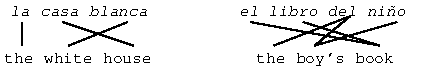
\includegraphics[scale=1]{brooke-localreorder}
\caption{When translating between Spanish and English, the positions
of nouns and their modifying adjectives are usually
swapped. Similarly, possessives in English generally precede nouns,
whereas in Spanish they follow the noun.}
\label{localreorder}
\end{figure}

The generalization capabilities of phrase-based systems are limited
due to their lack of direct, explicit knowledge of syntax. For
example, as we have seen, Spanish adjectives tend to follow the noun
they modify, a relative ordering that is the opposite of what is found
in English. But while phrase-based models can model this swapping more
easily than the IBM models can --- by essentially memorizing these
correspondences\footnote{The IBM models require the target phrase to
be a single word and therefore cannot memorize such correspondences.}
--- they have no mechanism for generalizing this phenomenon to novel
input phrases. Hence, if the phrase {\bold the purple apples} is seen
during testing but not training, the system is forced to translate the
words individually and relies on a different part of the system (i.e.,
another component model in the log-linear framework, such as the
distortion model) to make a prediction about their relative order.

Factor-based translation is equipped to make this kind of
generalization. These models can, for instance, make use of
part-of-speech information to express the fact that, even though {\em
the purple apples} has not been seen, the part-of-speech sequence {\em
determiner adjective noun} has been seen, and quite often its
translation has the part-of-speech sequence {\bold determiner noun
adjective}. Furthermore, if {\bold the purple apple} has been seen, the
framework has the ability to model the fact that {\bold apple} is the
lemma form of {\bold apples}; the system can therefore make use of the
translation {\bold las manzanas moradas} to derive the singular version
{\bold la manzana morada}. More often than not, in the face of novel
test strings, phrase-based systems to do not get the ordering
correct.

Preliminary experimental results from this summer's workshop indicate
that using factors can indeed improve translation performance. For
instance, we ran a number of experiments at this summer's workshop
that used morphological information when translating from English to
Spanish. The morphological features we used included those shown in
Table~\ref{morph}. The use of the morphology improved the BLEU score
by approximately 1.3 points over a phrase-based baseline (i.e., a
model without any added factor information), from 23.41 to 24.66
BLEU. This gain was induced by using a language model trained with
sequences in which the words of the original training data were
replaced by strings representing their morphological features. During
decoding, the factor-based model predicts the morphology of a
translation hypothesis, and the score of the morphological language
model is combined in the overall score of the hypothesis.

\begin{table}
\begin{center}
\begin{tabular}{|c|l|}
\hline
{\bf Category} & {\bf Attributes} \\
\hline
Adjective & gender, number \\
\hline
Determiner & gender, number, person, possessor \\
\hline
Noun & gender, number \\
\hline
Verb & gender, number, person, mode, tense \\
\hline
Pronoun & gender, number, person, case, possessor \\
\hline
\end{tabular}
\end{center}
\caption{The morphological features used in English-to-Spanish
translation experiments with a factor-based model.}
\label{morph}
\end{table}

\subsection{Motivation for a Syntax-Based Model}
While factor-based models show tremendous promise in solving some of
the gravest deficiencies of phrase-based systems, there remain some
problems that are unlikely to be addressed. During decoding, the
output of factor-based translation is constructed incrementally and
left-to-right. These partial translations are also scored
incrementally so as to make the computation tractable. This means that
the component models $h_i(e,f)$ in equation~\ref{loglinear} cannot
look globally at the translation to see whether it upholds global
syntactic constraints of the target language. For instance, it is
difficult to model the fact that in English, clauses usually have a
single finite verb and a subject.

The output in Table~\ref{SMTexamples} is taken from a state-of-the-art
phrase-based SMT system translating from German to English (the
baseline system described in \perscite{Collins2005}). This
system has been trained using over 700K sentence pairs from the
European Parliament dataset \parcite{koe:05}. These examples represent a
few of the syntactic errors this system tends to make. We consider
each example in turn, discussing some, but not all, of the problems:

\begin{itemize}
\item[1:] 
\begin{itemize}
\item[$\bullet$] In the first clause, the substring {\bold human rights practical}
introduces an unlikely ordering of a noun phrase {\bold human rights}
and adjective {\bold practical}.
\item[$\bullet$] In the second clause, there are two finite verbs ({\bold must} and
{\bold are}).
\end{itemize}
\item[2:]
\begin{itemize}
\item[$\bullet$] The clause beginning with {\bold the convention...} introduces two
adjacent noun phrases {\bold ...a draft a charter...}, which is an
unlikely event.
\item[$\bullet$] The prepositional phrase {\bold in the hands of the council}
appears before the verb it modifies ({\bold laid}), which is unusual in
English.
\item[$\bullet$] The verb phrase {\bold has formulated} has been split by elements
that normally would not split a verb phrase.
\item[$\bullet$] The adjective {\bold remarkable} is following the noun {\bold way}.
\item[$\bullet$] There is a missing referring pronoun ({\bold it}). I.e., the final
part of the sentence should say something like {\bold ...laid it in the
hands of the council}.
\end{itemize}
\item[3:]
\begin{itemize}
\item[$\bullet$] The infinitival phrase {\bold to maintain} follows its
noun phrase modifier.
\end{itemize}
\item[4:]
\begin{itemize}
\item[$\bullet$] The verb phrase {\bold will...erected} is not syntactically
well-formed (the insertion of the verb {\bold be} would make it so).
\end{itemize}
\item[5:]
\begin{itemize}
\item[$\bullet$] The first part of the sentence could be rendered as
two clauses {\bold it seems to us the budget perspectives are not
appropriate}, in which case there is a missing subject {\bold it} and a
missing verb {\bold are}; alternatively, it could be rendered as a
single clause {\bold the budget perspectives seem to us not
appropriate}, in which case the subject of the sentence has been
placed after the verb, and there is lack of agreement between the
subject and the verb.
\end{itemize}
\end{itemize}

While this output is taken from a phrase-based, and not a
factor-based, system, we argue that many of the syntactic errors,
particularly those that are global in nature, will not be corrected by
a factor-based system. For example, the misplacement of verbs with
respect to their modifiers, as in examples 2 and 3, is a very common
error. The problem stems from the fact that in independent clauses in
German, the finite verb is placed in the second position of the
sentence, and the infinitival verb, if it exists, is placed in the
final position. This means that in the English translation, the
infinitival verb may have to be moved across an arbitrary number of
intervening modifiers. Since phrase-based (and factor-based) systems
tend to either penalize translations that move phrases around too much
or to explicitly limit the absolute distance that phrases can move
(compromising the exactness of the search for efficiency), the output
tends mimic the word ordering of the input.

\begin{table}
\caption{Some examples of SMT output using a state-of-the-art
phrase-based system from German to English.}
\begin{center}
\begin{tabular}{p{2.25in}p{2.25in}}
{\bf SMT Output} & {\bf Reference Translation}\\
\hline
thus the implementation of human rights practical can be monitored , the union must have clear rules on possible penalties against the member states are available . & for the implementation of human rights to be monitored in practice also , however , the union must have clear rules regarding possible sanction mechanisms to be used against member states . \\
\hline
mr president , ladies and gentlemen , under the applause of the courts in luxembourg and strasbourg , the convention has a draft a charter of fundamental rights in a balanced way remarkable and formulated in the hands of the council laid . & mr president , ladies and gentlemen , with the approval of the courts in luxembourg and strasbourg , the convention has put together a draft charter of fundamental rights which is remarkably balanced , and has delivered it into the hands of the council . \\
\hline
i am with him that it is necessary , the institutional balance by means of a political revaluation of both the commission and the council to maintain . & i agree with him on the need to maintain the institutional balance and enhance the role , in political terms , of both the commission and the council . \\
\hline
irrespective of this , however , i should like to ask for this future is not already expect tomorrow , because they will gradually , stone for stone , erected . & that is why i invite you , in spite of everything , not to throw yourselves headlong into the future , as this is a future that should be built step by step , and stone by stone . \\
\hline
fifthly , seems to us the budget perspectives not appropriate... & fifthly , we also feel that the budgetary forecasts are not sufficient... \\
\hline
\end{tabular}
\end{center}
\label{SMTexamples}
\end{table}%

Other elements such as subjects and objects may also need to be
reordered to produce syntactically-sound output. Consider, for
instance, translation of the following German sentence into English:
{\bold f\"{u}r seinen bericht m\"{o}chte ich dem berichterstatter
danken}. The English translation of this sentence, {\bold i would like
to thank the rapporteur for his report}, involves a considerable
amount of reordering of the top-level phrases in the sentence (see
Figure~\ref{movement}): the subject {\bold ich} moves from after the
German modal verb {\bold m\"{o}chte} to the front of the English
translation; the prepositional-phrase modifier {\bold f\"{u}r seinen
bericht} moves from the front of the sentence to after the object in
the English.

\begin{figure}
\centering
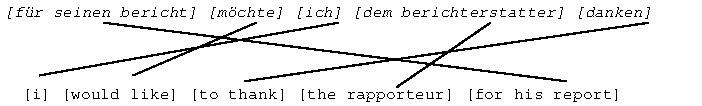
\includegraphics[scale=1]{brooke-movement}
\caption{The relative positioning of the top-level (bracketed) phrases
changes considerably in translation German to English.}
\label{movement}
\end{figure}

Figure~\ref{freeorder} shows three variations of the German sentence
introduced above with roughly the same meaning, illustrating how the
modifiers are relatively free to move around.\footnote{German is often
characterized as a {\bold V2} language due to the obligatory placement
of the finite verb in the second position in declarative sentences.}
In contrast, the placement of phrases in English is generally more
constrained: the subject of an English sentence is almost always
placed before the verb; the object almost always comes after the
verb. Hence, English is known as a predominantly {\em
subject-verb-object}, or {\bold S-V-O}, language. Therefore, when
translating from German to English, there is likely to be quite a bit
of reordering of top-level phrases.

\begin{figure}
\centering
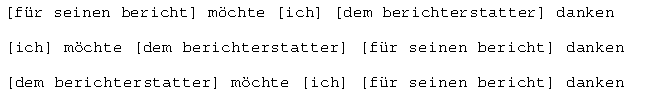
\includegraphics[scale=1]{brooke-freeorder}
\caption{In German, the top-level phrases can move around positionally
in the sentence without significantly altering its meaning. In the
example, the subject ({\bold ich}), object ({\bold dem berichterstatter}),
and a prepositional-phrase modifier ({\bold f\"{u}r seinen bericht})
exhibit such behavior.}
\label{freeorder}
\end{figure}

The reordering of top-level phrases can also be quite common when
translating between two fixed-word-order languages whose basic word
orders differ. For instance, Turkish, Japanese, and Korean, among many
of the world's other languages exhibit {\bold subject-object-verb} word
order. Figure~\ref{basicorder} shows how key sentential elements move
around in languages with different basic word orders.

\begin{figure}
\centering
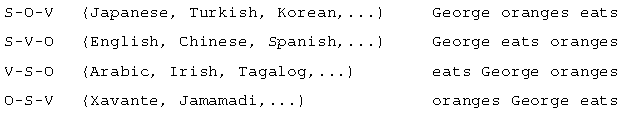
\includegraphics[scale=1]{brooke-basicorder}
\caption{The relative positions of the subject, verb, and object may
be different for different languages.}
\label{basicorder}
\end{figure}

Reordering poses a considerable challenge for phrase-based translation
systems. Factor-based systems have the potential to model reordering
based on, for instance, part of speech rather than words (i.e.,
factor-based distortion models). Indeed, some recent work has in fact
shown some improvement in translation quality by using part-of-speech
information in the distortion model \parcite{lia:06}. However, there are
other global syntactic constraints concerning the presence of
subjects, objects, verbs, and verbal modifiers, for instance, are
difficult to enforce within the phrase-based framework, and will very
likely be difficult to enforce within the factor-based framework as
well. Our observations of output produced by Moses this summer are
consistent with this conjecture. For instance, missing verbs in
sentences continues to be a problem with Moses, as it was with
Pharaoh.

Our syntax-based model makes predictions about the roles of top-level
phrases in the source-language input, as well as their positions in
the target-language output. This approach directly addresses the
global syntactic constraints, described above, which cannot easily be
modeled by a factor-based model. We propose using this model to
automatically reorder the input such that it more closely resembles
the syntactic ordering of the target language; we also propose making
use of the syntactic role information (e.g., {\bold subject}, {\em
object}, etc.) that the model predicts to better constrain the output
of the factor-based system. Finally, by translating certain parts of
the sentence prior to using the factor-based system, we intend to
ensure that certain essential parts of the sentence (such as the verb,
any wh-words or complementizers, etc.) appear in the output. Before
providing a detailed outline of our proposed integrated syntax and
factor based system, we describe our syntax-based model.

\section{The Syntax-Based Component}
\label{framework}

This section is based on work we have done at MIT CSAIL on a framework
for {\bold tree-to-tree} based statistical translation \parcite{cow:06}.
We focus here on one component of this framework: a model that
predicts {\bold aligned extended projections}, or AEPs. AEPs are derived
from the concept of an {\bold extended projection} in lexicalized tree
adjoining grammars (LTAG) \parcite{fra:02}, with the addition of
alignment information that is based on work in synchronous LTAG
\parcite{shisch:90}. The AEP model maps parse trees in the source
language to parse trees in the target language. We use a feature-based
model with a perceptron learning algorithm to learn this mapping. The
model is learned from a corpus of translation pairs, where each
sentence in the source or target language has an associated parse
tree.  We see two major benefits of tree-to-tree based
translation. First, it is possible to explicitly model the syntax of
the target language, thereby improving grammaticality. Second, we can
build a detailed model of the correspondence between the source and
target parse trees, thereby attempting to construct translations that
preserve the meaning of source language sentences.

Our AEP prediction framework involves a two-step process (described
below). We will use the German sentence {\bold wir wissen da\ss\,das
haupthemmnis der vorhersehbare widerstand der hersteller war} as a
running example. For this example we take the desired translation to
be {\bold we know that the main obstacle has been the predictable
resistance of manufacturers}.

\paragraph{Step 1:} The German sentence is parsed and then broken
down into separate parse structures for a sequence of clauses. For
example, the German example above is broken into a parse structure for
the clause {\bold wir wissen} followed by a parse structure for the
subordinate clause {\bold da\ss $\ldots$war}.

\paragraph{Step 2:} An AEP is predicted for
each German clause. To illustrate this step, consider translation of
the second German clause, which has the following parse structure:

\begin{small}
\begin{tabbing}
$\;$\hspace{1cm} s-oc \=kous-cp da\ss\\
       \>np-sb\avmbox{1} \= \=art das\\
                     \>\>\>nn haupthemmnis\\
       \>np-pd\avmbox{2} \> \>art der\\
                     \>\>\>adja vorhersehbare\\
                     \>\>\>nn widerstand\\
               \>\>np-ag \= \=art der\\
                               \>\>\>\>nn hersteller\\
       \>vafin-hd war
\end{tabbing}
\end{small}
Note that we use the symbols $\avmbox{1}$ and $\avmbox{2}$ to identify
the two modifiers (arguments or adjuncts) in the clause, in this case
a subject and an object.

A major part of the AEP is a parse-tree fragment, that is similar to a
TAG elementary tree (see also Figure~\ref{fig-aeps}):

\begin{center}
\begin{small}
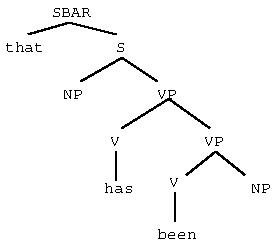
\includegraphics[scale=1]{brooke-AEP}
\end{small}
\end{center}


Following the work of \perscite{fra:02}, we will refer to a
structure like this as an {\bold extended projection} (EP). The EP
encapsulates the core syntactic structure in the English clause.  It
contains the main verb {\bold been}, as well as the function words {\em
that} and {\bold has}. It also contains a parse tree ``spine'' which has
the main verb {\bold been} as one of its leaves, and has the clause
label {\tt SBAR} as its root. In addition, it specifies positions for
arguments in the clause---in this case NPs corresponding to the
subject and object.

An AEP contains an EP, as well as {\bold alignment information} about
where the German modifiers should be placed in the extended
projection. For example, the AEP in this case would contain the tree
fragment shown above, together with an alignment specifying that the
modifiers $\avmbox{1}$ and $\avmbox{2}$ from the German parse will
appear in the EP as subject and object, respectively. In summary, an
AEP encapsulates the core syntactic structure of the English clause,
as well as information about where the translations of German
modifiers should appear.

AEPs are detailed structural objects, and their relationship to the
source-language clause can be quite complex. We use a discriminative
feature-based model, trained with the perceptron algorithm, to
incrementally predict the AEP in a sequence of steps. At each step we
define features that allow the model to capture a wide variety of
dependencies within the AEP itself, or between the AEP and the
source-language clause.

\subsection{Aligned Extended Projections (AEPs)}
\label{sec-aep}
We now provide a detailed description of AEPs.  Figure~\ref{fig-aeps}
shows examples of German clauses paired with the AEPs found in
training data.\footnote{Note that in this work we consider translation
from German to English; in the remainder of the section we take {\em
English} to be synonymous with the target language in translation and
{\bold German} to be synonymous with the source language.}  The German
clause is assumed to have $n$ (where $n \geq 0$) modifiers. For
example, the first German parse in Figure~\ref{fig-aeps} has two
arguments, indexed as $1$ and $2$. Each of these modifiers must either
have a translation in the corresponding English clause, or must be
deleted.

\begin{figure}
\begin{center}
\begin{small}
\begin{tabular}{|l|l|}
\hline
German Clause&English AEP\\
\hline
\hline
\parbox{1.5in}{
\begin{tabbing}
s-oc \=kous-cp da\ss\\
       \>np-sb\avmbox{1} \= \=art das\\
                     \>\>\>nn haupthemmnis\\
       \>np-pd\avmbox{2} \> \>art der\\
                     \>\>\>adja vorhersehbare\\
                     \>\>\>nn widerstand\\
               \>\>np-ag \= \=art der\\
                               \>\>\>\>nn hersteller\\
       \>vafin-hd war
\end{tabbing}

Paraphrase: {\bold that [np-sb the main obstacle] 
[np-pd the predictable resistance of manufacturers]
was}

}
&
\parbox{1.5in}{
\begin{tabbing}
STEM: be\\
SPINE:\\
\=SBAR-A \=IN that\\
                     \>\>S \=NP-A\\
                         \>\>\>VP \=V\\
                            \>\>\>\>NP-A\\
\end{tabbing}
\begin{tabbing}
VOICE:     \hspace{0.5cm}\=active\\
SUBJECT:   \>\avmbox{1}\\
OBJECT:    \>\avmbox{2}\\
MODALS:     \>has\\
INFL:      \>been\\
\end{tabbing}}\\
\hline
\hline
\parbox{1.5in}{
\begin{tabbing}
s   \=pp-mo\avmbox{1} \= \=appr zwischen\\
                    \>\>\>piat beiden\\
                    \>\>\>nn gesetzen\\
    \>vvfin-hd bestehen\\
    \>adv-mo\avmbox{2} also\\
    \>np-sb\avmbox{3} \> \>adja erhebliche\\
                \>\>\> \=adja rechtliche\\
                       \>\>\>\>\$, ,\\
                       \>\>\>\>adja praktische\\
                       \>\>\>\>kon und\\
                       \>\>\>\>adja wirtschaftliche\\
                \>\>\>nn unterschiede
\end{tabbing}

Paraphrase: {\bold [pp-mo between the two pieces of legislation] 
exist so [np-sb significant legal, practical and economic differences]}\\

}
&
\parbox{1.5in}{
\begin{tabbing}
STEM: be\\
SPINE:\\
S \= NP-A\\
  \>VP \= V\\
     \>\> NP-A\\
\end{tabbing}
\begin{tabbing}
VOICE:     \hspace{0.5cm}\=active\\
SUBJECT:   \>``there''\\
OBJECT:    \>\avmbox{3}\\
MODALS:     \>NULL\\
INFL:      \>are\\
MOD1: \> post-verb\\
MOD2: \> pre-sub\\
\end{tabbing}}\\
\hline
\hline
\parbox{1.5in}{
\begin{tabbing}
s-rc   \=prels-sb die\\
       \>vp \=pp-mo\avmbox{1} \= \=appr an\\
                         \>\>\>\>pdat jenem\\
                         \>\>\>\>nn tag\\
             \>\>pp-mo\avmbox{2} \> \=appr in\\
                           \>\>\>\>ne tschernobyl\\
               \>\>vvpp-hd gez\"{u}ndet\\
       \>vafin-hd wurde
\end{tabbing}

Paraphrase: {\bold which [pp-mo on that day] [pp-mo in chernobyl] released were}

}
&
\parbox{1.5in}{
\begin{tabbing}
STEM: release\\
SPINE:\\
SBAR \=WHNP\\
     \>SG-A VP V\\
\end{tabbing}
\begin{tabbing}
VOICE: \hspace{0.5cm}\=passive\\
WH:      \> which\\
MODALS:  \>  was\\
INFL:    \> released\\
MOD1:    \> post-verb  \\
MOD2:    \> post-verb
\end{tabbing}}\\
\hline
\end{tabular}
\end{small}
\end{center}
\caption{Three examples of German parse trees, together with their
  aligned extended projections (AEPs) in the training data. Note that AEP elements whose value is {\bold null} are not shown.
}
\label{fig-aeps}
\end{figure}

An AEP consists of the following parts:\footnote{Note that the
variables {\tt STEM}, {\tt SPINE}, {\tt VOICE}, {\tt WH}, {\tt
MODALS}, and {\tt INFL} essentially describe the EP of the English
main verb in the clause; the remaining variables {\tt SUBJECT}, {\tt
OBJECT}, and {\tt MOD(i)} specify the position of modifiers in the
German clause.}

\paragraph{STEM:} A string specifying the stemmed form of the
main verb in the clause.

\paragraph{SPINE:} A syntactic structure associated with the main verb. 
  The structure has the symbol {\tt V} as one of its leaf nodes; this
  is the position of the main verb. It includes higher projections of
  the verb such as VPs, Ss, and SBARs. It also includes leaf nodes
  {\tt NP-A} in positions corresponding to noun-phrase arguments
  (e.g., the subject or object) of the main verb. In addition, it may
  contain leaf nodes labeled with categories such as {\tt WHNP} or
  {\tt WHADVP} where a wh-phrase may be placed. It may include leaf
  nodes corresponding to one or more complementizers (common examples
  being {\bold that}, {\bold if}, {\bold so that}, and so on).

\paragraph{VOICE:} One of two alternatives, {\tt active} or 
{\tt passive}, specifying the voice of the main verb.

\paragraph{SUBJECT:} This variable can be one of three types. If there
is no subject position in the {\tt SPINE} variable, then the value for
{\tt SUBJECT} is {\tt NULL}. Otherwise, {\tt SUBJECT} can either be a
string, for example {\bold there},\footnote{This happens in the case
where there exists a subject in the English clause but not in the
German clause. See, for instance, the second example in
Figure~\ref{fig-aeps}.} or an index of one of the $n$ modifiers in the
German clause.

\paragraph{OBJECT:} This variable is similar to {\tt SUBJECT}, and can
also take three types: {\tt NULL}, a specific string, or an index of
one of the $n$ German modifiers. It is always {\tt NULL} if there is
no object position in the {\tt SPINE}; it can never be a modifier
index that has already been assigned to {\tt SUBJECT}.

\paragraph{WH:} This variable is always {\tt NULL} if there is no
wh-phrase position within the {\tt SPINE}; it is always a
non-empty string (such as {\bold which}, or {\bold in which}) if a
wh-phrase position does exist.

\paragraph{MODALS:} This is a string of verbs that constitute the
modals that appear within the clause. We use {\tt NULL} to signify
that there are no modals.

\paragraph{INFL:} The inflected form of the verb.

\paragraph{MOD(i):} There are $n$ modifier variables {\tt
  MOD(1), MOD(2), $\ldots$, MOD(n)} that specify the positions for
German arguments that have not already been assigned to the {\tt
SUBJECT} or {\tt OBJECT} positions in the spine. Each variable {\tt
MOD(i)} can take one of five possible values:

\begin{itemize}
\item {\tt null}: This value is chosen if and only if the modifier has
  already been assigned to the subject or object position.
\item {\tt deleted}: This means that a translation of the $i$'th
  German modifier is not present in the English clause.
\item {\tt pre-sub}: The modifier appears after any complementizers or
  wh-phrases, but before the subject of the English clause.
\item {\tt post-sub}: The modifier appears after the subject of the
  English clause, but before the modals.
\item {\tt in-modals}: The modifier appears after the first modal in
  the sequence of modals, but before the second modal or the main
  verb. 
\item {\tt post-verb}: The modifier appears somewhere after the main
  verb. 
\end{itemize}


\subsection{A Discriminative Model for AEP Prediction}
\label{sec-model}
In this section we describe linear history-based models with beam
search, and the perceptron algorithm for learning in these
models. These methods will form the basis for our model that maps
German clauses to AEPs.

We have a training set of $n$ examples, $(x_i,y_i)$ for $i = 1 \ldots
n$, where each $x_i$ is a German parse tree, and each $y_i$ is an AEP.
We follow previous work on history-based models, by representing each
$y_i$ as a series of $N$ decisions $\langle d_1, d_2, \ldots d_N
\rangle$. In our approach, $N$ will be a fixed number for any input
$x$: we take the $N$ decisions to correspond to the sequence of
variables {\tt STEM, SPINE, $\ldots$, MOD(1), MOD(2), $\ldots$,
MOD(n)} described in section~\ref{sec-aep}.  Each $d_i$ is a member of
a set ${\cal D}_i$ which specifies the set of allowable decisions at
the $i$'th point (for example, ${\cal D}_2$ would be the set of all
possible values for {\tt SPINE}).  We assume a function
$\hbox{ADVANCE}(x, \langle d_1, d_2, \ldots, d_{i-1} \rangle)$ which
maps an input $x$ together with a prefix of decisions $d_1 \ldots
d_{i-1}$ to a subset of ${\cal D}_i$. $\hbox{ADVANCE}$ is a function
that specifies which decisions are allowable for a past history
$\langle d_1, \ldots, d_{i-1} \rangle$ and an input $x$. In our case
the $\hbox{ADVANCE}$ function implements hard constraints on AEPs (for
example, the constraint that the {\tt SUBJECT} variable must be {\tt
NULL} if no subject position exists in the {\tt SPINE}).  For any
input $x$, a {\bold well-formed} decision sequence for $x$ is a sequence
$\langle d_1, \ldots, d_N \rangle$ such that for $i = 1 \ldots n$,
$d_i \in \hbox{ADVANCE}(x, \langle d_1, \ldots, d_{i-1} \rangle)$. We
define $\gen(x)$ to be the set of all decision sequences (or AEPs)
which are well-formed for $x$.

The model that we will use is a discriminatively-trained,
feature-based model. A significant advantage to feature-based models
is their flexibility: it is very easy to sensitize the model to
dependencies in the data by encoding new features.  To define a
feature-based model, we assume a function $\rep(x, \langle d_1,
\ldots, d_{i-1} \rangle, d_i) \in \reals^d$ which maps a decision
$d_i$ in context $(x, \langle d_1, \ldots, d_{i-1} \rangle)$ to a {\em
feature vector}. We also assume a vector $\pav \in \reals^d$ of
parameter values. We define the {\bold score} for any partial or
complete decision sequence $y = \langle d_1, d_2, \ldots, d_m \rangle$
paired with $x$ as:
\begin{equation}
\hbox{SCORE}(x,y) = \ip{\Rep(x,y)}{\pav}
\label{eq-score}
\end{equation}
where
$
\Rep(x,y) = 
\sum_{i=1}^m \rep(x,\langle d_1, \ldots, d_{i-1} \rangle, d_i)
$.
In particular, given the definitions above, the output structure
$F(x)$ for an input $x$ is the highest--scoring well--formed structure for $x$:
\begin{equation}
F(x) = \arg\max_{y \in \gen(x)} \hbox{SCORE}(x,y)
\label{eq-argmax}
\end{equation}
To decode with the model we use a beam-search method. The method
incrementally builds an AEP in the decision order $d_1, d_2, \ldots,
d_N$. At each point, a beam contains the top $M$ highest--scoring
partial paths for the first $m$ decisions, where $M$ is taken to be a
fixed number. The score for any partial path is defined in
Eq.~\ref{eq-score}. The $\hbox{ADVANCE}$ function is used to specify
the set of possible decisions that can extend any given path in the
beam.

To train the model, we use the averaged perceptron algorithm described
by \perscite{col:02}.  This combination of the perceptron
algorithm with beam-search is similar to that described by \perscite{colroa:04}.\footnote{Future work may consider
alternative algorithms, such as those described by \perscite{daumar:05}.} The perceptron algorithm is a convenient
choice because it converges quickly --- usually taking only a few
iterations over the training set \parcite{col:02,colroa:04}.

\subsection{The Features of the Model}
\label{sec-feats}

The model's features allow it to capture dependencies between the AEP
and the German clause, as well as dependencies between different
parts of the AEP itself. The features included in $\rep$ can
consist of any function of the decision history $\langle d_1, \ldots,
d_{i-1} \rangle$, the current decision $d_i$, or the German clause. In
defining features over AEP/clause pairs, we make use of some basic
functions which look at the German clause and the AEP (see
Tables~\ref{GERfunc} and \ref{AEPfunc}). We use various combinations
of these basic functions in the prediction of each decision $d_i$, as
described below.

\begin{table}[!h]
\begin{center}
\begin{small}
\begin{tabular}{|c|l|}
\hline
1 & main verb \\
\hline
2 & any verb in the clause \\
\hline
3 & all verbs, in sequence \\
\hline
4 & spine \\
\hline
5 & tree \\
\hline
6 & preterminal label  of left-most child of subject \\
\hline
7 & terminal label of left-most child of subject \\
\hline
8 & suffix of terminal label of right-most child of subject \\
\hline
9 & preterminal label  of left-most child of object \\
\hline
10 & terminal label of left-most child of object \\
\hline
11 & suffix of terminal label of right-most child of object \\
\hline
12 & preterminal label of the negation word {\bold nicht} ({\bold not}) \\
\hline
13 & is either of the strings {\bold es gibt} ({\bold there is/are})\\
& or {\bold es gab} ({\bold there was/were}) present? \\
\hline
14 & complementizers and wh-words \\
\hline
15 & labels of all wh-nonterminals \\
\hline
16 & terminal labels of all wh-words \\
\hline
17 & preterminal label of a verb in first position \\
\hline
18 & terminal label of a verb in first position \\
\hline
19 & terminal labels of all words in any relative pronoun\\
&  under a PP \\
\hline
20 & are all of the verbs at the end? \\
\hline
21 & nonterminal label of the root of the tree \\
\hline
22 & terminal labels of all words constituting the subject \\
\hline
23 & terminal labels of all words constituting the object \\
\hline
24 & the leaves dominated by each node in the tree \\
\hline
25 & each node in the context of a CFG rule \\
\hline
26 & each node in the context of the RHS of a CFG rule \\
\hline
27 & each node with its left and right sibling \\
\hline
28 & the number of leaves dominated by each node \\
&in the tree \\
\hline
\end{tabular}
\end{small}
\end{center}
\caption{Functions of the German clause used for making features in
the AEP prediction model.}
\label{GERfunc}
\end{table}

\begin{table}[!h]
\begin{center}
\begin{small}
\begin{tabular}{|c|l|}
\hline
1 & does the {\tt SPINE} have a subject? \\
\hline
2 & does the {\tt SPINE} have an object? \\
\hline
3 & does the {\tt SPINE} have any wh-words? \\
\hline
4 & the labels of any complementizer nonterminals \\
& in the {\tt SPINE} \\
\hline
5 & the labels of any wh-nonterminals in the {\tt SPINE} \\
\hline
6 & the nonterminal labels {\tt SQ} or {\tt SBARQ} in the {\tt SPINE} \\
\hline
7 & the nonterminal label of the root of the {\tt SPINE} \\
\hline
8 & the grammatical category of the finite verbal form\\
 &  {\tt INFL} (i.e., infinitive, 1st-, 2nd-, or 3rd-person pres,\\
& pres participle, sing past, plur past, past participle) \\
\hline
\end{tabular}
\end{small}
\end{center}
\caption{Functions of the English AEP used for making features
in the AEP prediction model.}
\label{AEPfunc}
\end{table}

\paragraph{STEM:} 
Features for the prediction of {\tt STEM} conjoin
the value of this variable with each of the functions in lines 1--13
of Table~\ref{GERfunc}.  For example, one feature is the value of {\tt
STEM} conjoined with the main verb of the German clause. In addition,
$\rep$ includes features sensitive to the rank of a
candidate stem in an externally-compiled lexicon.\footnote{The lexicon
is derived from GIZA++ and provides, for a large number of German main
verbs, a ranked list of possible English translations.}

\paragraph{SPINE:} 
Spine prediction features make use of the values of the variables {\tt
SPINE} and {\tt STEM} from the AEP, as well as functions of the spine
in lines 1--7 of Table~\ref{AEPfunc}, conjoined in various ways with
the functions in lines 4, 12, and 14--21 of Table~\ref{GERfunc}. Note
that the functions in Table~\ref{AEPfunc} allow us to look at
substructure in the spine. For instance, one of the features for {\tt
SPINE} is the label {\tt SBARQ} or {\tt SQ}, if it exists in the
candidate spine, conjoined with a verbal preterminal label if there is
a verb in the first position of the German clause. This feature
captures the fact that German yes/no questions begin with a verb in
the first position.

\paragraph{VOICE:} 
Voice features in general combine values of {\tt VOICE}, {\tt SPINE},
and {\tt STEM}, with the functions in lines 1--5, 22, and 23 of
Table~\ref{GERfunc}.

\paragraph{SUBJECT:} 
Features used for subject prediction make use of the AEP variables
{\tt VOICE} and {\tt STEM}. In addition, if the value of {\tt SUBJECT}
is an index $i$ (see section~\ref{sec-aep}), then $\rep$ looks at the
nonterminal label of the German node indexed by $i$ as well as the
surrounding context in the German clausal tree. Otherwise, $\rep$
looks at the value of {\tt SUBJECT}. These basic features are combined
with the functions in lines 1, 3, and 24--27 of Table~\ref{GERfunc}.

\paragraph{OBJECT:} 
We make similar features to those for the prediction of {\tt
SUBJECT}. In addition, $\rep$ can look at the value predicted for
{\tt SUBJECT}.

\paragraph{WH:} 
Features for {\tt WH} look at the values of {\tt WH} and {\tt SPINE},
conjoined with the functions in lines 1, 15, and 19 of
Table~\ref{GERfunc}.

\paragraph{MODALS:} 
For the prediction of {\tt MODALS}, $\rep$ looks at {\tt MODALS}, {\tt
SPINE}, and {\tt STEM}, conjoined with the functions in lines 2--5 and
12 of Table~\ref{GERfunc}.

\paragraph{INFL:} 
The features for {\tt INFL} include the values of {\tt INFL}, {\tt
MODALS}, and {\tt SUBJECT}, and {\tt VOICE}, and the function in line
8 of Table~\ref{AEPfunc}.

\paragraph{MOD(i):} 
For the {\tt MOD(i)} variables, $\rep$ looks at the value of {\tt
MODALS}, {\tt SPINE} and the current {\tt MOD(i)}, as well as the
nonterminal label of the root node of the German modifier being
placed, and the functions in lines 24 and 28 of Table~\ref{GERfunc}.

\subsection{Experiments with the AEP Model}
We implemented an end-to-end system for translation from German to
English using our AEP prediction model as a component. The Europarl
corpus \parcite{koe:05} constituted our training data. This corpus
contains over 750,000 training sentences; we extracted over 441,000
training examples for the AEP model from this corpus (see
\parcite{cow:06} for details on the extraction of these training
examples). We reserved 35,000 of these training examples as
development data for the model. We used a set of features derived from
the those described in section~\ref{sec-feats}. This set was optimized
using the development data through experimentation with several
different feature subsets.

Modifiers within German clauses were translated using the phrase-based
model of \perscite{koe:03}. We first generated $n$-best
lists for each modifier. We then built a reranking model to choose
between the elements in the $n$-best lists. The reranker was trained
using around 800 labeled examples from a development set.

The test data for the experiments consisted of 2,000 sentences, and
was the same test set as that used by \perscite{Collins2005}. We use the model of \perscite{koe:03} as a baseline for our experiments. The
AEP-driven model was used to translate all test set sentences where
all clauses within the German parse tree contained at least one verb
and there was no embedding of clauses---there were 1,335 sentences
which met these criteria. The remaining 665 sentences were translated
with the baseline system. This set of 2,000 translations had a BLEU
score \parcite{pap:02} of 23.96. The baseline system alone achieved a
BLEU score of 25.26 on the same set of 2,000 test sentences. We also
obtained judgments from two human annotators on 100 randomly-drawn
sentences on which the baseline and AEP-based outputs differed.  For
each example the annotator viewed the reference translation, together
with the two systems' translations presented in a random order.
Annotator 1 judged 62 translations to be equal in quality, 16
translations to be better under the AEP system, and 22 to be better
for the baseline system. Annotator 2 judged 37 translations to be
equal in quality, 32 to be better under the baseline, and 31 to be
better under the AEP-based system.

\section{A Syntax and Factor Based Model for SMT}
\label{future}
In the preceding section, we presented a model that predicts detailed
target-language syntactic structures, which include constraints on the
alignments between source and target parse trees. In this work, we
intend to implement a model that integrates our syntax-based system
and the factor-based system Moses. The integration involves using the
syntax-based system to predict the syntactic roles of constituents in
the source-language input, and reorder them before they are translated
using Moses. In addition, the syntax-based system would be used to
translate certain parts of the input and ensure that they appear in
the target language output. We would like to test this integrated
model with German-to-English translation, as well as
Spanish-to-English and English-to-Spanish translation. The work with
Spanish and English will form a natural continuation of the work we
performed translating from English to Spanish this summer at the
workshop. Although the primary focus of this work will be on the
integration with Moses, we see the need for improvement of our AEP
model. We hope such improvements will contribute to better quality
translations produced by the integrated system. Finally, we envision
implementation of a few alternative approaches to end-to-end
translation using the AEP model; we expect to use these alternatives
as points of comparison with the integrated approach. The next few
sections describe our proposed integration with Moses, some additional
motivations for investigating Spanish-English translation, the
AEP-prediction improvements that we anticipate carrying out, and the
alternative end-to-end translation systems.

\subsection{Integration with a Factor-Based System}
The end-to-end translation framework we have developed in previous
work uses a phrase-based system to produce $n$-best lists of modifier
translations, which are then reranked and placed into the final
translation. By selecting modifier translations independently, we are
failing to make use of valuable contextual information that could be
used to form better translations.  Rather than produce modifier
translations in isolation, we can use the syntax-based system to
produce modified MT input to the phrase-based
system. Figure~\ref{modifiedinput} illustrates how the input to the MT
system is rearranged by the syntax-based AEP model. Note that in step
two of the figure, some of the input has been translated to English
(the verb sequence {\bold would like to thank}), while some if it has
merely been reordered. This allows the phrase-based system to decode
the entire AEP at once.

\begin{figure}
\begin{center}
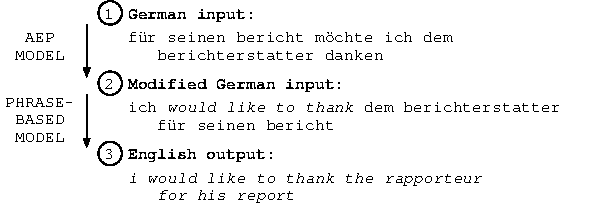
\includegraphics[scale=1.2]{brooke-modifiedinput2}
\end{center}
\vspace{-0.5cm}
\caption{The input to the MT system --- {\bold f\"{u}r seinen bericht
m\"{o}chte ich dem berichterstatter danken} --- is rearranged by the
syntax-based system to produced modified input to the phrase-based
system.}
\label{modifiedinput}
\end{figure}

An approach similar to this one has been investigated in previous work
using hand-written reordering rules, which improved translation
quality when compared with a phrase-based baseline system
\parcite{Collins2005}. Our current work differs from the previous work in
several significant ways:

\begin{itemize}
\item our work is carried out entirely within a statistical
framework, whereas the earlier work used hand-coded deterministic
rules for reordering;
\item our work attempts to identify the roles of target-language
output phrases and account for them in the source-language input,
whereas the previous work attempted only to reorder the input; the
prediction of grammatical functions such as {\bold subject} and {\em
object} can be used as additional input to the phrase-based system
(see below);
\item our work explicitly tries to account for the existence and
translation of certain sentence elements such as complementizers,
wh-words, and main verbs;
\end{itemize}

In addition to the simple reordering of input suggested in
Figure~\ref{modifiedinput}, we envision several extensions. We might,
for instance, try training language models specific to the syntactic
roles predicted by the AEP model (e.g., subject, object, verbal
modifier). These language models could be incorporated into the
factor-based framework as additional features in the model. The use of
such language models would be motivated by the desire to have the
model learn something about the structure of a ``subject'', for
instance (e.g., that a subject should probably look like a noun
phrase).

This particular line of investigation raises many interesting research
questions related to the reordering of top-level phrases (i.e.,
modifiers):

\begin{itemize}
\item Does it help to disallow reordering of the top-level phrases in
the modified input to the phrase-based system (i.e., implement a hard
constraint on reordering)?  Or, is it better to implement a soft
constraint on reordering (for example by penalizing the reordering of
modifiers)?  Or, is it better not to impose any constraints on
reordering at all?
\item How much language engineering is necessary to extract a
reasonable subset of possible permutations of top-level phrases in the
input?  How well can the phrase-based decoder do by simply taking into
account all possible reorderings while decoding? (Note that if
arbitrary reorderings of words in the sentence are allowed, the
decoding problem is NP-complete \parcite{kni:99}.) Do we really need to
use a full parse, or can we devise a model that uses only syntactic
chunking (partial parsing) or semantic role labeling?
\item Can we simplify the role of the first (preprocessing) step,
perhaps by (1) learning a mapping from source-sentence elements to
target-sentence roles (subject, object, modifier, verb,
complementizer), and then (2) learning an ordering on those elements?
Note that this approach implies that no part of the input to the
phrase-based system would be translated by the syntax-based system.
\end{itemize}

\subsection{Other Language Pairs: Spanish/English}
We would like to test the integrated syntax and factor based system
with language pairs other than German/English, and for translation
into a language besides English.  One language pair that we are
interested in working with is Spanish/English. Spanish is interesting
for a number of reasons \parcite{zag:02}:

\begin{itemize}
\item it has a fairly rich morphology, with subjects and verbs
agreeing in number and person, and the nouns, determiners, and
adjectives in a noun phrase agreeing in number and gender;
\item constituent order is not fixed in declarative sentences
(constituents may appear as S-V-O, V-O-S, or V-S-O);
\item if understood from context, the subject does not have to appear
in a sentence;
\item the use of the subjunctive mood is quite prevalent and may be
triggered by a phrase that appears far away from the inflected verb;
\item the passive voice is used in many cases where active voice would
be the natural choice in English;
\item Spanish uses two forms of past tense (preterite and imperfect)
where English uses only one (simple);
\item Spanish has two forms of the verb {\bold to be};
\item Spanish uses double clitics (that is, two clitics with the same
referent), and there are two possible positions when placing clitics
in sentences where a verb appears in the progressive or infinitive
form.
\end{itemize} 

From a research perspective, one of the benefits of our approach is
that we can leverage the relatively recent advances in parsing
languages other than English (e.g.,
\parcite{chibik:02,arukel:04,col:99b,cowcol:05}). We have developed a
statistical parser for Spanish \parcite{cowcol:05} that we intend to use
for this project. The parser makes use of morphological information
and reranking techniques to achieve, on test data, an F1 score of
85.1\% in the recovery of labeled constituents.  The parser is
currently trained on only 2800 sentences; this number will increase by
a factor of 10 with the release of new data at the end of 2006.

\subsection{Improved AEP Prediction}
Improvements in the accuracy with which the AEP model predicts AEPs
will almost certainly lead to improved translation quality, and can
only reduce the amount of work that the factor-based system has to
do. We have analyzed several random samples of output from our current
system in an attempt to characterize its current
performance. Table~\ref{errors} shows examples of some of the errors
we have observed:

\begin{enumerate}
\item {\bf subject/verb agreement}: In English, the subject and verb
must agree in number. In the example, the verb {\bold to be} is
inflected for plurality, while the subject is singular.
\item {\bf subject choice}: The AEP model predicts there is no
subject, or mispredicts the alignment of the subject. In the example,
the second clause of the sentence ({\bold while believe on the same side
of the political spectrum}) is missing a subject.
\item {\bf object choice}: The AEP model predicts there is no object,
or (more commonly) mispredicts the alignment of the object. In the
example, the true object --- {\bold position} --- in the last clause
({\bold to take in his second speech to this issue position}) is
incorrectly predicted as a modifier and is placed after the object.
\item {\bf number finite verbs}: The system occasionally produces more
than one finite verb per clause. In the example, the final clause
({\bold we will come in future this is often}) contains two finite
verbs, {\bold come} and {\bold is}. The reason for this is usually that
the phrase-based system introduces a new finite verb in translating of
one of the modifiers.
\item {\bf preposition choice}: Either a preposition is missing, or
the choice of preposition is incorrect. In the example, the
preposition {\bold at} has been selected; a more appropriate choice
would have been {\bold on}.
\end{enumerate}

\begin{table}
\caption{Examples of some common errors in the output of our syntax-based system.}
\begin{center}
\begin{tabular}{p{.8in}|p{1.85in}p{1.85in}}
{\bf Error Type} & {\bf System Output} & {\bf Reference Translation}\\
\hline subject/verb agreement & the council are denied any power of legislating . & the council is denied any power of legislating .\\
\hline subject choice & mr blair sees the precondition for more liberalisation while believe on the same side of the political spectrum , this is the prerequisite for the development of a social europe & mr blair sees this as the condition for greater liberalisation , while others , on the same side of the political chessboard , believe that it is the condition for the advent of social europe \\
\hline object choice & i hope very that the prime minister sets it positive apart and would ask him if it does to take in his second speech to this issue position & i would like to hope that the prime minister will address it positively and i should like , if he can , for him to take a position on this issue in his second speech . \\
\hline number finite verbs & this annex is and i know we will come in future this is often & this is to be welcomed , and i know we will return to this many times in the future .\\
\hline preposition choice & i should like to comment at the thessaloniki agenda in the areas of immigration and asylum& mr president , i am going to refer to the thessaloniki agenda in relation to immigration and asylum .\\
\hline
\end{tabular}
\end{center}
\label{errors}
\end{table}

It is clear from this list that the prediction of particular parts of
the AEP could be improved. For instance, subjects and objects are
often not accurately predicted. In addition, we have routinely
observed that the choice of the main verb is often not optimal or even
correct. Based on our informal observations, it seems to be the case
that high-accuracy AEP prediction is correlated with high-accuracy
translation output. We intend to produce by hand a set of gold
standard AEPs which could be used to generate and score
translations. The difference between generating translations using the
gold-standard AEPs and generating translations using the predicted
AEPs will give us a more quantitative idea of the loss incurred by the
mispredictions.

The feature-driven approach allows a wide range of features to be
tested in attempting to improve AEP prediction accuracy. For example,
it would be relatively easy to incorporate a syntactic language model
(i.e., a prior distribution over AEP structures) induced from a large
amount of English monolingual data. Future work may also consider
alternative definitions of AEPs. For example, we might consider AEPs
that include larger chunks of phrase structure, or we might consider
AEPs that contain more detailed information about the relative
ordering of modifiers.

Alternative learning methods might improve the accuracy of the
model. For example, a large-margin optimization technique such as the
exponentiated gradient approach to structured prediction \parcite{bar:04}
might be adapted to the AEP prediction problem. We might also look
into improving how training examples are extracted, for instance, by
looking into a better method for extracting and aligning clause pairs
and modifiers. Our current method involves heuristics for determining
modifier alignment; this might be done instead by using the EM
algorithm to induce the best alignment.

\subsection{Alternative End-to-End Systems}
We foresee implementing at least two alternative translation systems
using our AEP model. One of these systems uses finite state machines
to represent alternative modifier translations; it is closer in nature
to our current modifier-reranking framework, although we have reason
to believe it will perform better than our current implmentation. The
other alternative involves a recursive application of the AEP model to
modifier translation.

\paragraph{Using finite state machines}
Rather than using the phrase-based system to produce $n$-best lists of
translations, we can use it to produce finite state machines (FSM)
representing a network of possible translations (see, e.g.,
\parcite{moh:97}). It is then easy to create an integrated AEP-FSM, in
which the conjunctions and other substrings of the translation derived
from the AEP are also represented as finite-state machines. We could
then take the intersection of the AEP-FSM with an $n$-gram language
model, for instance. Selecting modifiers using this representation
would correspond to searching the finite-state network for the most
likely path. Crucially, this search would take into account the
contextual information that is being thrown away in our current
reranking approach. It would also incorporate a language model over
the entire sentence. The current system uses a language model only
when producing modifier translation candidates with the phrase-based
system. Finally, the FSM framework facilitates the incorporation of
any additional models that can be encoded using a finite-state
representation. For instance, we might train language models for
particular types of modifiers predicted by the AEP (e.g., subject,
object, etc).

\paragraph{Recursive prediction of modifier AEPs}
\label{recursive}
According to most (if not all) syntactic theories, classes of words
other than verbs (such as nouns, adjectives, and prepositions) can
also subcategorize lexically for certain types of arguments, and can
influence their distributions \parcite{haegue:99}. Similarly, extended
projections may be formed for many types of words besides verbs. A
natural extension to the current AEP model, then, is the application
of AEP prediction to the translation of modifiers. For example, given
a German modifier aligned to the English subject, we may try to
predict a corresponding AEP, which would likely involve the extended
projection of a noun. Exactly how we would form the modifier AEPs (for
instance for prepositional phrases) would be part of this work.

This approach is compelling for a couple of reasons:

\begin{itemize}
\item it facilitates the modeling of syntactic structure conditioned
on the intended role (subject, object, etc) of the target-language modifier;
\item it offers an AEP framework that is entirely self-contained,
without reliance on a phrase-based system.
\end{itemize}


This system is quite different from the integrated syntax and factor
based system and should therefore make a very interesting point of
comparison.

\subsection{Summary}
The goal of this research is to integrate a system that makes explicit
use of global syntactic information with one that is able to
incorporate factors in a phrase-based framework. We aim to use the
mutual strengths of each system to produce high-quality automatic
translations. We intend to test our model using German/English and
Spanish/English language pairs. In addition, we plan to implement
several improvements to the AEP prediction model, as well some
alternative end-to-end translation models that make use of the AEP
model and can act as points of comparison to the integrated syntax and
factor based model. We hope that this work will not only produce
better machine translation output, but will also help elucidate how
syntactic information can best be used for SMT.


\chapter{Detailed Results for the Czech-English Experiments}\label{czech-appendix}

{  % wrapping all Ondrej's content to prevent confusing macros
%{\sc Ond\v{r}ej Bojar}


\def\clap#1{\hbox to 0pt{\hss #1\hss}}
\def\equo#1{``#1''}
\def\ang#1{{$\langle${#1}$\rangle$}}  % snadny zapis spicatych zavorek
\def\text#1{{\it{}#1}}


\def\bidir{Czech$\leftrightarrow$English}
\def\tocs{English$\rightarrow$Czech}
\def\toen{Czech$\rightarrow$English}
\def\parcite#1{(\cite{#1})}
\def\perscite#1{\cite{#1}} % works like newcite

\def\max#1{{\bf{} #1}}
\def\stddev#1{{$\pm$#1}}


\def\subsubsubsection#1{\bigskip{}{\it #1\\}}


This appendix goes into great detail about the \bidir{} translation  experiments that were described in a summarized form in Section \ref{czech-english-summary}.

Section \ref{data} describes the data used for our experiments, including
preprocessing steps and some basic statistics. Section \ref{baselines}
introduces the metric and lists some known result on MT quality on our
dataset, including the scores of human translation. The core of this report is
contained in Section \ref{experiments} where all our experiments and results are
described in detail.




\section{Data Used}
\label{data}




\subsection{Corpus Description and Preprocessing}
\label{tools}


The data used for \bidir{} experiments are available as CzEng 0.5
\parcite{czeng:pbml:2006} and PCEDT 1.0 \parcite{pcedt:2004}. The collection contains parallel texts from various domains, as
summarized in Table~\ref{czengratios}.


\begin{table}[ht]
\begin{tabular}{lrr|rr}
  &  \multicolumn{2}{c}{Sentences}  &  \multicolumn{2}{c}{Tokens}\\
  &  Czech                             &  English                          &  Czech  &  English\\
\hline
Texts from European Parliament         &  77.7\%  &  71.7\%  &  78.2\%  &  75.9\%\\
E-Books                                &  5.5\%   &  6.6\%   &  7.2\%   &  7.4\%\\
KDE (open-source documentation)        &  6.9\%   &  10.2\%  &  2.6\%   &  3.6\%\\
PCEDT-WSJ (Wall Street Journal texts)  &  1.5\%   &  1.7\%   &  2.6\%   &  2.8\%\\
Reader's Digest stories                &  8.4\%   &  9.7\%   &  9.4\%   &  10.3\%\\
\hline
Total                                  &  1.4 M   &  1.3 M   &  19.0 M  &  21.6 M\\
\end{tabular}
\caption{Domains of texts contained in full training data.}
\label{czengratios}
\end{table}

The texts in CzEng are pre-tokenized and pre-segmented (sentence boundaries identified) and
automatically sentence-aligned using the hunalign tool
\parcite{varga:hunalign:2005}. The
PCEDT data are manually sentence aligned 1-1 by origin, because the Czech
version of the text was obtained by translating English text sentence by
sentence.

For the purposes of our experiments, we processed the data using the tools
listed in Table \ref{toolsused}.
The English side of the corpus had to be retokenized (keeping CzEng sentence
boundaries), because the original tokenization was not compatible with the tagging tool.

\begin{table}[ht]
\begin{center}
\small
\begin{tabular}{lcc}
  &  Czech  &  English\\
\hline
Segmentation  &  CzEng  &  CzEng\\
Tokenization  &  CzEng  &  \clap{Like Europarl, \cite{koe:05}}\\
Morph./POS Tagging  &  \cite{hajhla:1998b}  &  \cite{mxpost:1996}\\
Lemmatization  &  \cite{hajhla:1998b}  &  -not used-\\
Parsing  &  \cite{mcdonald:pereira:ribarov:hajic:2005}  &  -not used-\\
\end{tabular}
\end{center}
\caption{Czech and English tools used to annotate CzEng data.}
\label{toolsused}
\end{table}



\subsection{Baseline (PCEDT) and Large (CzEng+PCEDT) Corpus Data}
\label{baselinelargecorpus}

The evaluation set of sentences used in our experiments (see section
\ref{references} below) comes from the very specific domain of Wall Street
Journal. The PCEDT-WSJ section matches this domain exactly, so we
use the PCEDT-WSJ section (20k sentences) as the training data in most of our experiments and refer
to it by the term \equo{baseline corpus} or simply PCEDT. In some
experiments, we make use of all the training data (860k sentences) and refer to it as the
\equo{large corpus}. (Of course, test data
are always excluded from training.)



\begin{table}[t]
\begin{center}
\begin{tabular}{llrrr}
Corpus  &    &  Sentences  &  Tokens\\
\hline
Baseline: PCEDT  &  Czech    &  20,581   &  453,050\\
                 &  English  &  20,581   &  474,336\\
\hline
Large: CzEng+PCEDT     &  Czech    &  862,398  &  10,657,552\\
                 &  English  &  862,398  &  12,001,772\\
\end{tabular}
\end{center}
\caption{Data sizes available for our experiments.}
\label{corpsizes}
\end{table}

Table \ref{corpsizes} reports exact data sizes of the baseline and large
corpora used for our experiments. (Note that the baseline corpus is a subset of
the large corpus.) The data size is significantly lower than what CzEng offers,
because not all of the sentences successfully passed through all our tools and
also due to the removal of sentences longer than 50 words and sentences with the ratio
between Czech and English number of tokens worse than 9.


% Including possible other data (licensing problems):
%File        	Sentences	Tokens
%forbidden.cs	1,030,872	12,339,260
%forbidden.en	1,030,872	13,894,186

%Data: /export/ws06osmt/data/cs-en/training 



\subsection{Tuning and Evaluation Data}
\label{references}


Our tuning and evaluation data consist of 515 sentences
with 4 reference
translations. The dataset was first published as part of PCEDT 1.0 for
evaluating \toen{} translation and included original English Wall Street
Journal (WSJ) texts translated to Czech (sentence by sentence) and 4 independent
back-translations to English. For the purposes of \tocs{} translation in our experiments, another 4
independent translations from the original English to Czech were obtained.

For our experiments we kept the original division of the dataset into two parts: the
tuning (development) set and the evaluation test set.
However, we retokenized all the sentences with the Europarl
tokenization tool. Dataset sizes in terms of number of sentences, input tokens
and input tokens never seen in the PCEDT training corpus (out-of-vocabulary,
OOV) are listed in Table \ref{tuneevaldata}.

\begin{table}[ht]
\begin{center}
\begin{tabular}{lccccc}
  &    &  \multicolumn{4}{c}{Input Tokens When Translating from}\\
   &  Sentences   &  Czech  &  OOV   &  English  &  OOV\\
\hline
Tuning   &  259  &  6429  &  6.8\%  &  6675  &  3.5\%\\
Evaluation  &  256  &  5980  &  6.9\%  &  6273  &  3.8\%\\
\end{tabular}
\end{center}
\caption{Tuning and evaluation data.}
\label{tuneevaldata}
\end{table}

We followed the common procedure to use tuning dataset to set parameters of the
translation system and to use the evaluation dataset for final translation
quality estimate. In other words, the translation system has access to the
reference translations of the tuning dataset but never has access to the
reference translations of the evaluation dataset.

In the following, we use the this short notation: \equo{Dev (std)} denotes
results obtained on the tuning dataset with the model parameters set to the
default, somewhat even distribution. \equo{Dev (opt)} denotes results on the
tuning dataset with the parameters optimized using minimum error rate training
procedure (see section \ref{merttuning}). The \equo{Dev (opt)} results are always overly
optimistic, because MERT had access to the reference translations and tunes the
MT output to get the highest scores possible. \equo{Test
(opt)} denotes results on evaluation set with model parameters as optimized on
the tuning set. The \equo{Test (opt)} results thus estimate the system
performance on unseen data and allow for a fair comparison.

For the purposes of automatic translation, the input texts were analyzed using
the same tools as listed in section \ref{tools}.



\section{MT Quality Metric and Known Baselines}
\label{baselines}

Throughout all our experiments, we use the BLEU metric \parcite{pap:02}
to automatically assess the quality of translation. We use an implementation of
this metric provided for the workshop. Other implementations such as IBM
original or NIST official {\tt mt\_eval} might give slightly
different absolute results, mainly due to different tokenization rules.

In all experiments reported below, we train and test the system in
{\it case-insensitive} fashion (all data are converted to lowercase, including
the reference translations), except where stated otherwise.



\subsection{Human Cross-Evaluation}

Table \ref{crosseval} displays the scores if we evaluate one human translation
against 4 other human translations. For the sake of completeness, we report not
only the default lowercase (LC) evaluation but also case sensitive (CSens)
evaluation. This estimate cannot be understood as any kind of a bound or limit
on MT output scores, but it nevertheless gives some vague orientation when
reading BLEU figures.

\begin{table}[ht]
\begin{center}
\begin{tabular}{llccc|ccc}
   &     &  \multicolumn{3}{c}{To Czech}   &  \multicolumn{3}{c}{To English}\\
  &    &  Min  &  Average  &  Max  &  Min  &  Average  &  Max\\
\hline
Evaluation   &  LC   &  38.5  &  43.1$\pm$4.0  &  48.4   &  41.6  &  54.5$\pm$8.4  &  62.9\\
   &  CSens  &  38.1  &  42.5$\pm$4.0  &  47.8   &  41.1  &  53.8$\pm$8.4  &  62.4\\
\hline
Tuning   &  LC   &  39.0  &  46.3$\pm$4.3  &  49.3   &  45.8  &  55.3$\pm$6.0  &  61.7\\
   &  CSens  &  38.3  &  45.8$\pm$4.4  &  48.8   &  45.0  &  54.7$\pm$6.1  &  61.3\\
\end{tabular}
\end{center}
\caption{BLEU scores of human translation against 4 different human
translations. Evaluated 5 times, always comparing one translation against the 4
remaining. The minimum, average and maximum scores of the 5-fold estimation are
given.}
\label{crosseval}
\end{table}

As expected, we observe a higher variance (standard deviation) when evaluating
translation to English. The reason is that one of the five English versions of
the sentences is the original, while the other four were back translated
from Czech. It is therefore quite likely for the four back translations to differ
more from the original than from each other raising the BLEU variance.

English scores are generally higher and this may indicate that there is less variance
in word order, lexical selection or word morphology in English, but it also
could be the simple case that the translators to English produced more rigid
translations.


\subsection{BLEU When not Translating at All}

Our particular type of text (WSJ) contains a lot of numbers and proper names
that are often not altered during translation. Just for curiosity and to 
check that our datasets are not just numbers, punctuation and company names, we
evaluate BLEU for texts not translated at all. I.e. the input text is evaluated
against the standard 4 references. As displayed in Table
\ref{nontransl}, the scores are very low but nonzero, as expected.

\begin{table}[ht]
\begin{center}
\begin{tabular}{llcc}
   &     &  To Czech   &  To English\\
\hline
Evaluation   &  Lowercase   &  2.20  &  2.66\\
Evaluation   &  Case Sensitive   &  2.20  &  2.65\\
Tuning   &  Lowercase   &  2.93  &  3.60\\
Tuning   &  Case Sensitive   &  2.93  &  3.59\\
\end{tabular}
\end{center}
\caption{BLEU scores when not translating at all, i.e. only punctuation, numbers
and some proper names score.}
\label{nontransl}
\end{table}


\subsection{Previous Research Results}

Table \ref{comparison} summarizes previously published results of \toen{}
translation. Dependency-based MT (DBMT, \perscite{cmejrek:curin:havelka:2003})
is a system with rule-based transfer from Czech deep syntactic trees (obtained
automatically using one of two parsers of Czech) to English
syntactic trees. GIZA++ \parcite{och:ney:2003} and ReWrite
\parcite{rewrite:germann:2003} is the \equo{standard
baseline} word-based statistical system.
PBT \parcite{zens:etal:pbt:2005} is a phrase-based statistical
MT system developed at RWTH Aachen that has been evaluated on English-Czech data
by \perscite{bojar:etal:fintal:2006}.


\begin{table}[ht]
\begin{center}
\begin{tabular}{l@{\quad}c@{\quad}c@{\quad}|@{\quad}c@{\quad}c}
  &  \multicolumn{2}{@{\hspace{-1em}}c@{\quad}|@{\quad}}{Average over 5 refs.}  &  \multicolumn{2}{@{\quad}c}{4 refs. only}\\
%  &  \multicolumn{2}{c@{\quad}|@{\quad}}{Average  over four}  &  \multicolumn{2}{@{\quad}c@{\quad}}{Four re-translations}\\
%  &  \multicolumn{2}{c@{\quad}|@{\quad}}{re-translations + original}  &  \multicolumn{2}{@{\quad}c}{only}\\
  &  Dev  &  Test  &  Dev  &  Test\\
\hline
DBMT with parser I, no LM            &    18.57  &     16.34  &  -  &  -\\
DBMT with parser II, no LM           &    19.16  &     17.05  &  -  &  -\\
GIZA++ \& ReWrite, bigger LM         &    22.22  &     20.17  &  -  &  -\\
\hline                                   
PBT, no additional LM                &    38.7\stddev{1.5}  &  34.8\stddev{1.3}  &  36.3  &     32.5\\
PBT, bigger LM                       &    41.3\stddev{1.2}  &  36.4\stddev{1.3}  &  39.7  &     34.2\\
\hline                                                                                    
PBT, more parallel texts, bigger LM  &    42.3\stddev{1.1}  &  38.1\stddev{0.8}  &  41.0  &     36.8\\
\end{tabular}
\end{center}
\caption{Previously published results of \toen{} MT.}
\label{comparison}
\end{table}

All figures in Table \ref{comparison} are based on the same training dataset as
we use: the baseline corpus of PCEDT (20k sentences) and on the same tuning and
evaluation sets. However, the tokenization of the data is slightly different the
we use and also a different implementation of the BLEU metric was used. Our
experience is that a different scoring script can change BLEU results by about 2
points absolute, so these numbers should not be directly compared to our results
reported here.

Unlike \perscite{cmejrek:curin:havelka:2003} who evaluate
four-reference BLEU
five times using the original English text in addition to the 4 available
reference back-translations in a leave-one out procedure, we always report BLEU
estimated on the 4 reference translations only.


To the best of our knowledge, we are the first to evaluate \tocs{} machine
translation quality with automatic measures.




\section{Experiments}
\label{experiments}



\subsection{Motivation: Margin for Improving Morphology}
\label{margin}

Czech is a Slavonic language with very rich morphology and relatively free word
order. (See e.g. \perscite{bojar:cslp:2004} for more details.) The Czech
morphological system defines 4,000 tags in theory and 2,000 were actually seen
in a big tagged corpus. (For comparison, the English Penn Treebank tagset
contains just about 50 tags.) When translating to Czech, any MT system has to
face the richness and generate output words in appropriate forms.

Table \ref{morphmargin} displays BLEU scores of single-factored translation
\tocs{} using the baseline corpus only. The second line in the table gives the
scores if morphological information was disregarded in the evaluation: the MT
output is lemmatized (word forms replaced with their respective base forms) and evaluated against lemmatized references.

\begin{table}[ht]
\begin{center}
\begin{tabular}{lccc}
%     &  pcedt .t0-0. t0-0 LM0-3-pcedt  &                &            &  \\
  &  Dev (std)  &  Dev (opt)  &  Test (opt)\\
\hline
Regular BLEU, lowercase  &  25.68  &  29.24  &  25.23\\
Lemmatized MT output\\
\quad{}against lemmatized references  &  34.29  &  38.01  &  33.63\\
%margin:  &  8.61  &  8.77  &  8.40\\
\end{tabular}
\end{center}
\caption{Margin in BLEU for improving morphology.}
\label{morphmargin}
\end{table}

We see that more than 8 point BLEU absolute could be achieved if output word
forms were chosen correctly.\footnote{Although not all required word forms may
be available in the training data, we could easily generate output word forms
from lemmas and morphological tags deterministically using a large
target-side-only dictionary.} This observation gives us a strong motivation for
focussing on morphological errors first.



\subsection{Obtaining Reliable Word Alignment}

Given the richness of Czech morphological system and quite limited amount of
data in the baseline corpus (20k sentences), our first concern was to obtain
reliable word alignments. Like \perscite{bojar:etal:fintal:2006}, we reduce the
data sparseness by either lemmatizing or stemming Czech tokens and stemming
English tokens. (By stemming we mean truncating each word to at most 4
characters.) The vocabulary size of Czech word forms reduces to a half after
stemming or lemmatization and comes thus very close to the vocabulary size of English
word forms.

Table \ref{alignments} displays BLEU scores on Test (opt) \tocs{} depending on the
preprocessing of corpus for word alignment. The translation process itself was
performed on full word forms (single-factored), with a single trigram language
model collected from the Czech side of the parallel corpus. In all cases, we employed the
grow-diag-final heuristic for symmetrization of two independent GIZA++ runs.


\begin{table}[ht]
\begin{center}
\begin{tabular}{cccc}
\multicolumn{2}{c}{Preprocessing for Alignment}  &  \multicolumn{2}{c}{Parallel Corpus Used}\\
English          &  Czech       &  Baseline (20k sents.)  &  Large (860k sents.)\\
\hline
word forms       &  word forms  &                  25.17  &  -\\
4-char stems  &  lemmas      &                  25.23  &                25.40\\
4-char stems            &  4-char stems       &                  25.82  &                24.99\\
\end{tabular}
\end{center}
\caption{BLEU in \tocs{} translation depending on corpus preprocessing for word
alignment.}
\label{alignments}
\end{table}

The results confirm improvement in translation quality if we address the data
sparseness problem for alignments either by full lemmatization or by simple
stemming.  Surprisingly, using full lemmatization of the Czech side scored worse
than just stemming Czech. This result was confirmed neither on the large
training set, nor by \perscite{bojar:etal:fintal:2006} for \toen{} direction, so
we attribute this effect to random fluctuations in MERT procedure.

We also see nearly no gain or even some loss by increasing the corpus size
from 20k to 860k sentences. (See section \ref{moredata}
below for more details on various ways of using more data.)
This observation can be explained by the very specific
domain of our test set.


\subsection{Scenarios of Factored Translation \tocs{}}


\subsubsection{Scenarios Used}

We experimented with the following factored translation scenarios:

%\begin{tabular}{c@{\hspace{1cm}}c}
%English  &  Czech\\
%\hline
%\Rnode{elc}{lowercase}  &  \Rnode{clc}{lowercase}\\
%\end{tabular}
%\psset{nodesep=5pt,arrows=->}
%\everypsbox{\scriptstyle}
%\ncLine{elc}{clc}


\piccaption{Single-factored scenario (T).}
\parpic[fr]{%
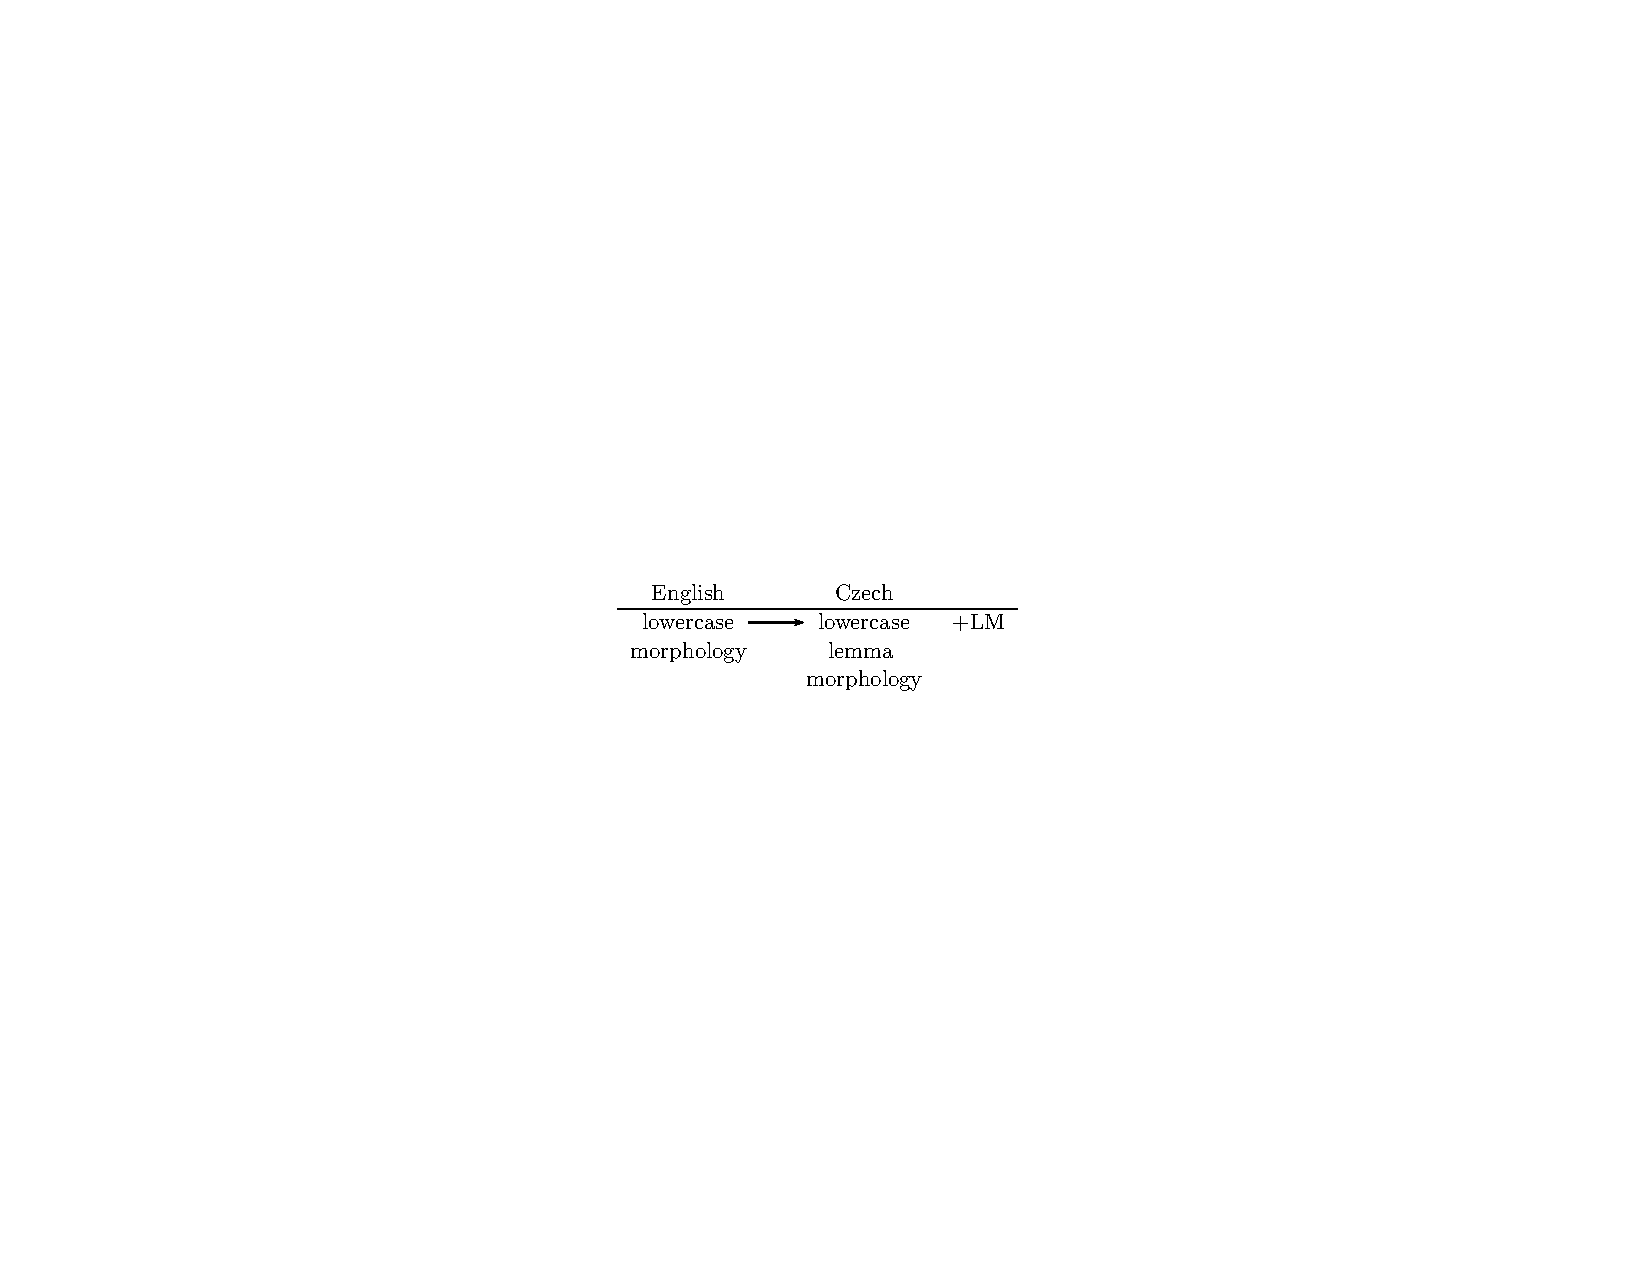
\includegraphics{images/ondrej-picture-1}
}

The baseline scenario is single-factored: input (English) lowercase word forms
are directly translated to target (Czech) lowercase forms. A 3-gram language
model (or more models based on various corpora) checks the stream of output word forms.

We call this the \equo{T} (translation) scenario.


\piccaption{Checking morphology (T+C).}
\parpic[fr]{%
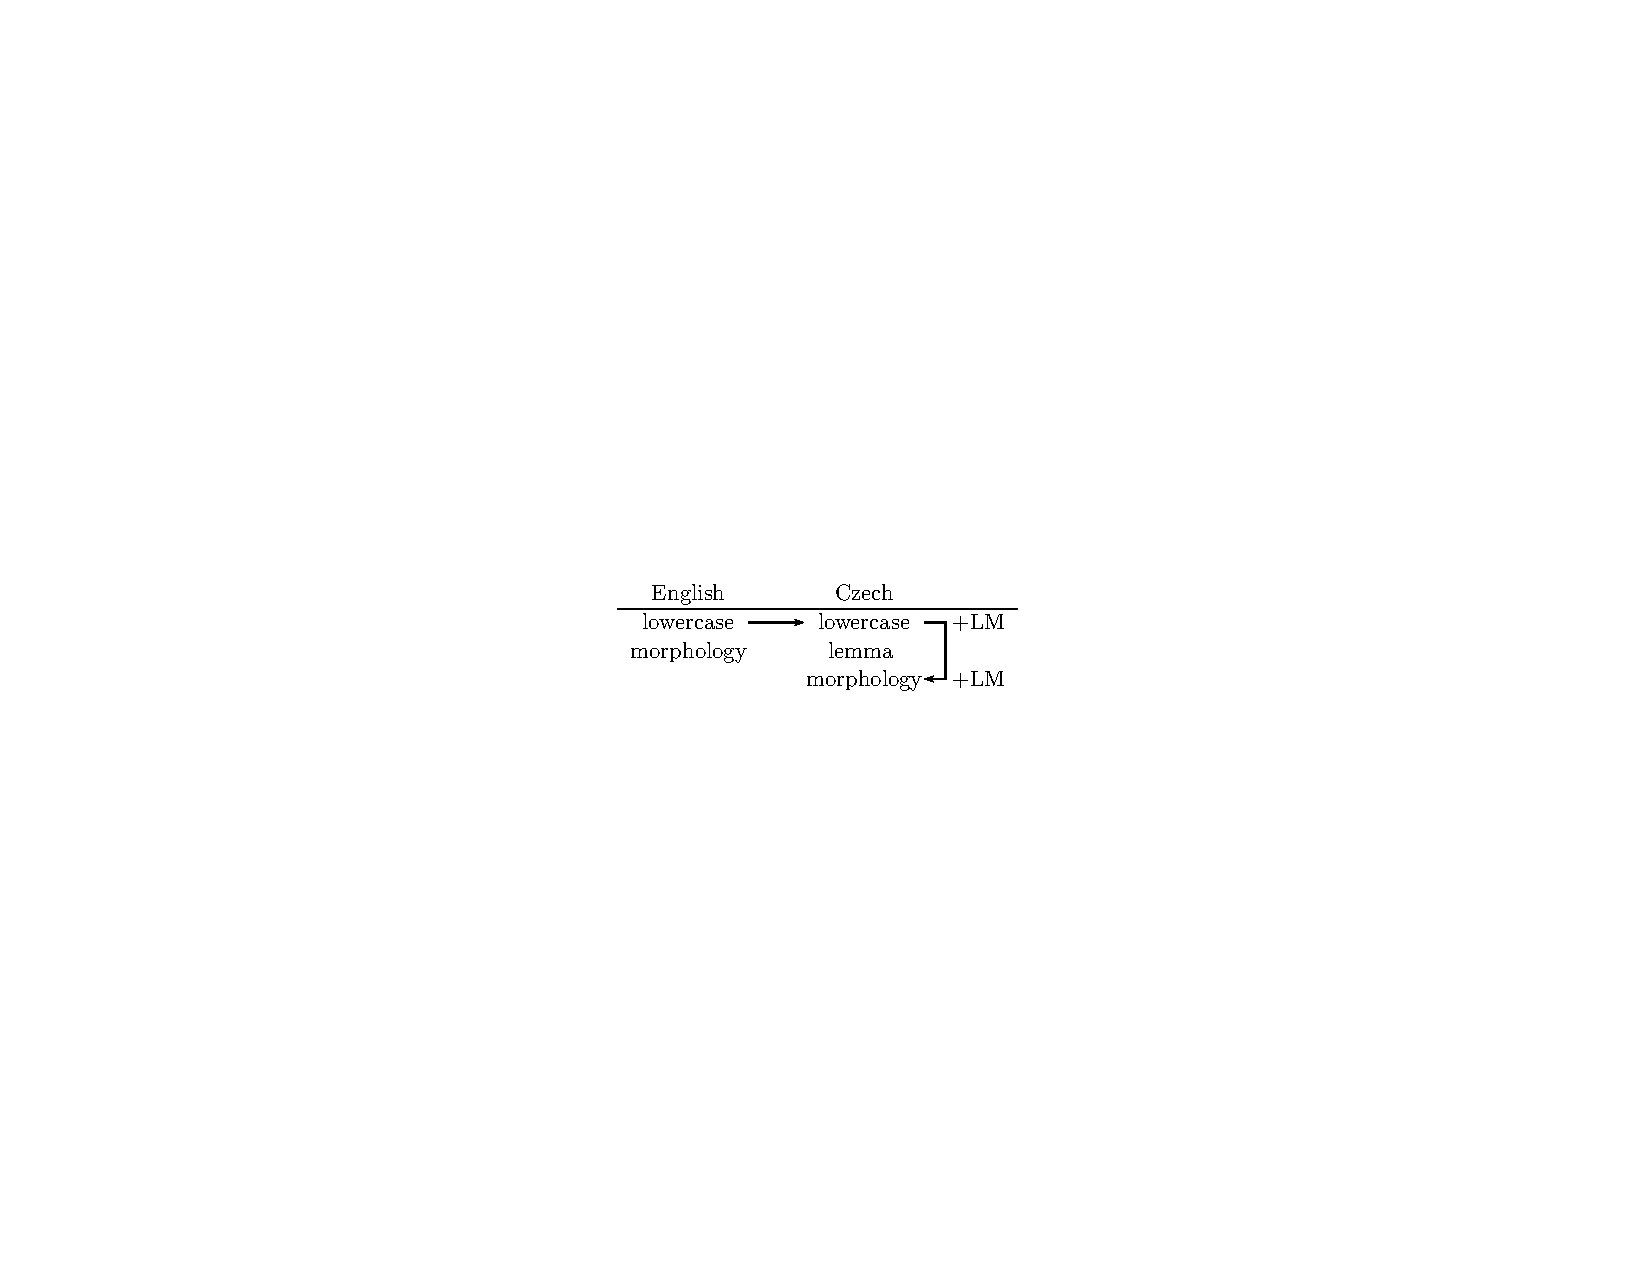
\includegraphics{images/ondrej-picture-2}
}


In order to check the output not only for word-level coherence but also
for morphological coherence, we add a single generation step: input word forms
are first translated to output word forms and each output word form then
generates its morphological tag.

Two types of language models can be used simultaneously: a (3-gram) LM over word forms and a
LM over morphological tags. For the morphological tags, a higher-order LM can be
used, such as 7 or 9-gram.

We used tags with various levels of detail, see section \ref{posgranularity}.
We call this the \equo{T+C} (translate and check) scenario.


\piccaption{Translating and checking morphology (T+T+C).}
\parpic[fr]{
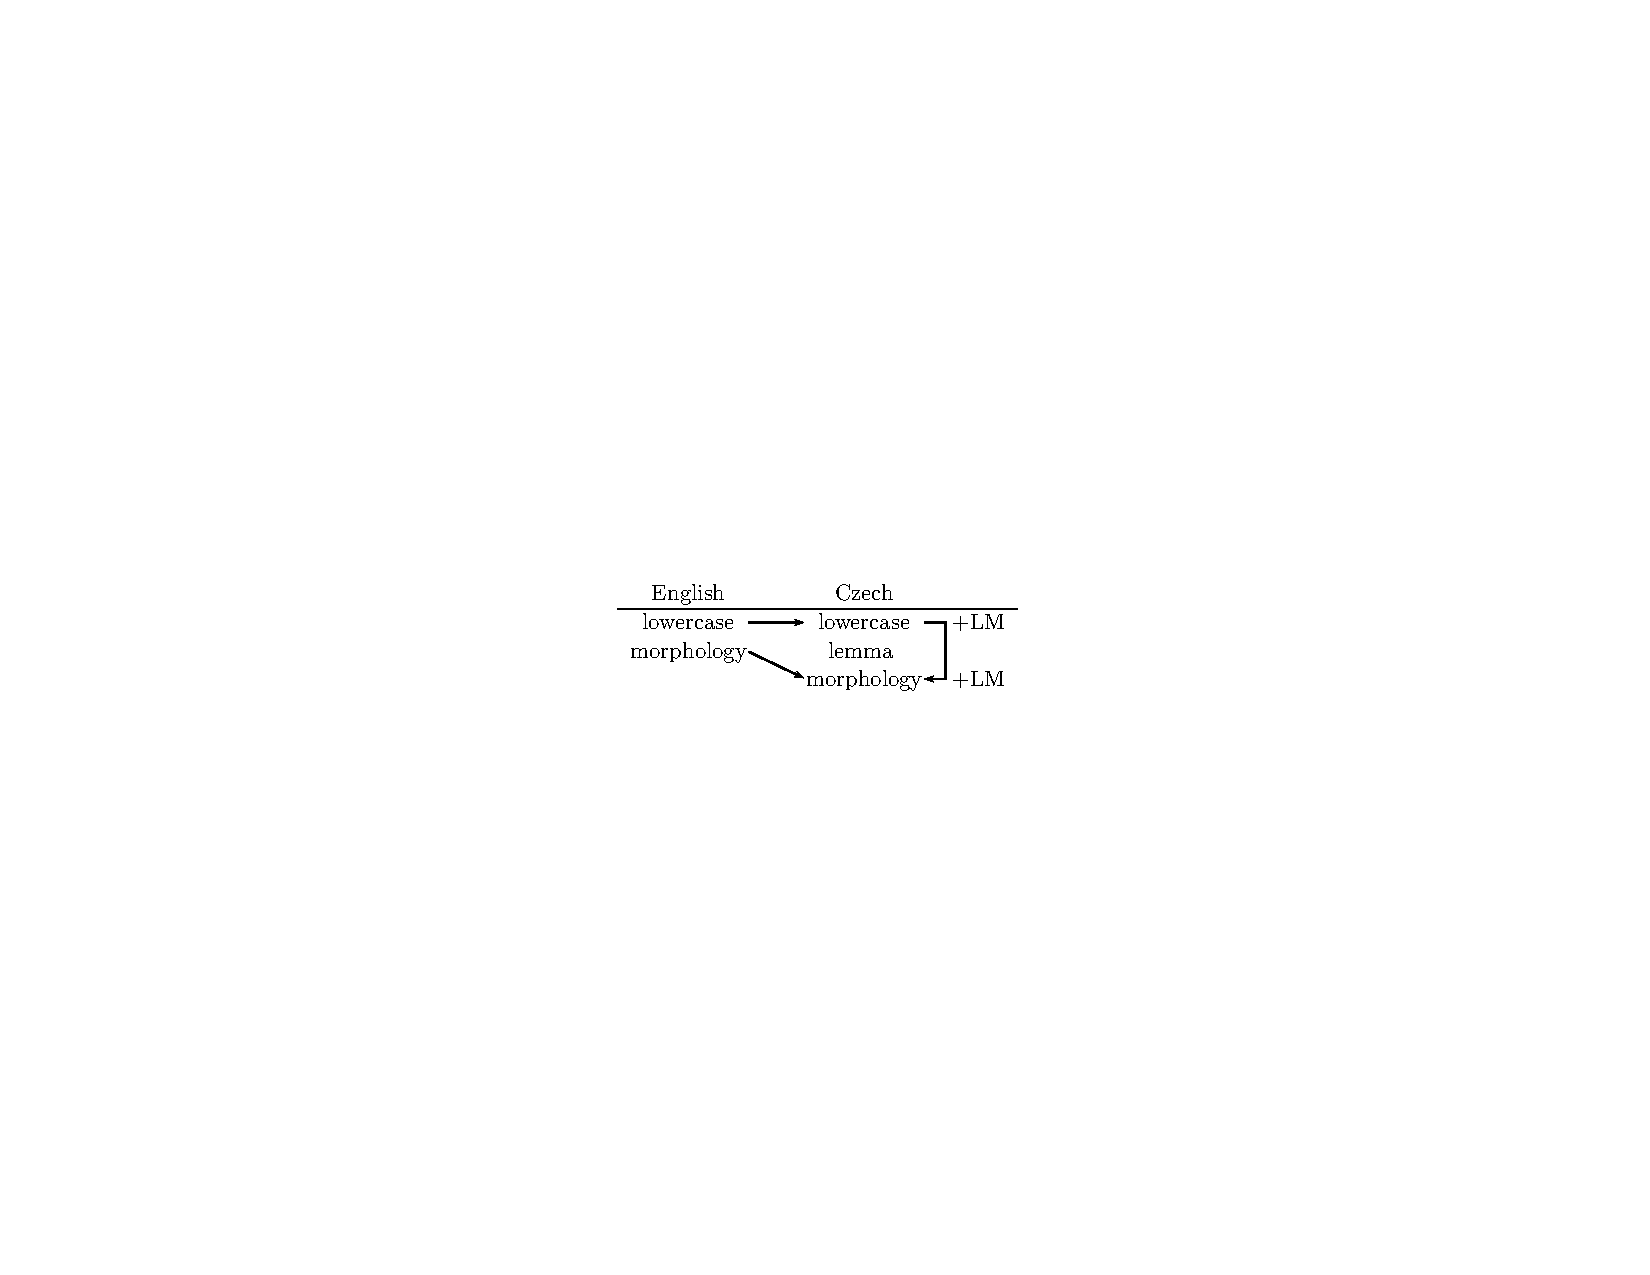
\includegraphics{images/ondrej-picture-3}}

As a refinement of T+C, we also used T+T+C scenario, where the morphological
output stream is constructed based on both, output word forms and input
morphology. This setting should ensure correct translation of morphological
features such as number of source noun phrases.
%, while the T+C setting simply guessed number of noun
%phrases based on the language models.

Again, two types of language models can be used in this \equo{T+T+C} scenario.

\piccaption{Generating forms from lemmas and tags (T+T+G).}
\parpic[fr]{%
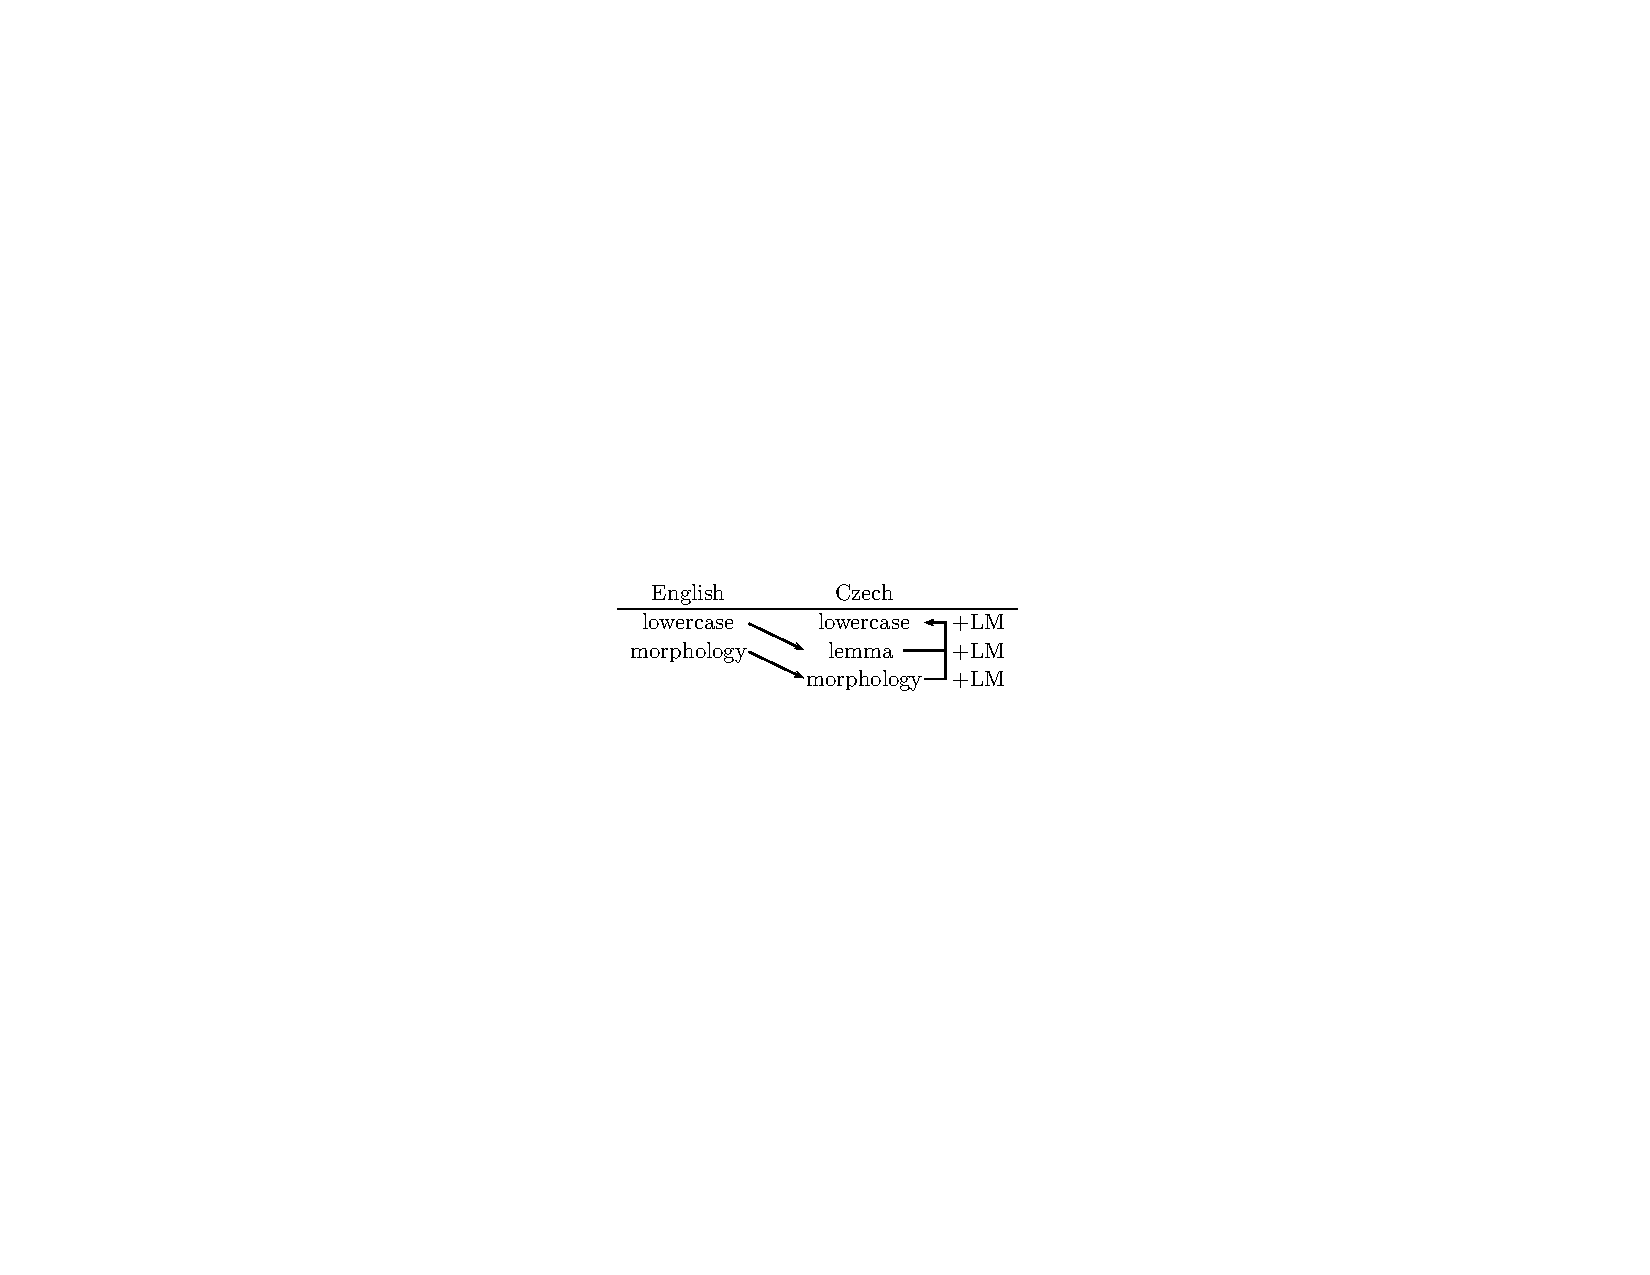
\includegraphics{images/ondrej-picture-4}}

The most complex scenario we used is linguistically appealing: output lemmas
(base forms) and morphological tags are generated from input in two independent
translation steps and combined in a single generation step to produce
output word forms. The input English text was not lemmatized so we used English
word forms as the source for producing Czech lemmas.

The \equo{T+T+G} setting allows us to use up to three types of language models.
Trigram models are used for word forms and lemmas and 7 or 9-gram language
models are used over tags.



%% small pictures
%\psset{unit=5mm}
%\begin{pspicture}(0,-0.5)(3,0.5)
%\psline{->}(0,0)(3,0)
%\pscircle*[fillcolor=white](0,0){0.5ex}
%\end{pspicture}
%
%\psset{unit=5mm}
%\begin{pspicture}(0,-0.5)(3,1.5)
%\psline{->}(0,1)(3,1)
%\psline{->}(3,1)(3,0)
%\end{pspicture}
%
%\psset{unit=5mm}
%\begin{pspicture}(0,-0.5)(3,2.5)
%\psline{->}(0,2)(3,2)
%\psline{->}(0,1)(3,0)
%\psline{->}(3,2)(3,0)
%\end{pspicture}
%
%
%\psset{unit=5mm}
%\begin{pspicture}(0,-0.5)(3,2.5)
%\psline{->}(0,2)(3,1)
%\psline{->}(0,1)(3,0)
%\psline{->}(3,1)(3.5,1)(3.5,2)(3,2)
%\psline{->}(3,0)(3.5,0)(3.5,2)(3,2)
%\end{pspicture}



\subsubsection{Experimental Results: T+C Works Best}

Table \ref{scenariosresults} summarizes estimated translation quality of the
various scenarios. In all experiments, only the baseline corpus of 20k sentences
was used with word alignment obtained using grow-diag-final heuristic on stemmed
English and lemmatized Czech input streams. Language models are also based
on the 20k sentences only, 3-grams are used for word forms and lemmas, 7-grams
for morphological tags.


\begin{table}[ht]
\begin{center}
\begin{tabular}{lccc}
  &  Dev (std)  &  Dev (opt)  &  Test (opt)\\
\hline
Baseline: T      &  25.68  &  29.24  &  25.23\\
T+T+G  &  23.93  &  30.34  &  25.94\\
T+T+C  &  25.12  &  30.73  &  26.43\\
T+C    &  23.51  &  \max{30.88}  &  \max{27.23}\\
\end{tabular}
\end{center}
\caption{BLEU scores of various translation scenarios.}
\label{scenariosresults}
\end{table}

The good news is that multi-factored models always outperform the baseline T
(except for \equo{Dev (std)}, but this is not surprising, as the default weights
can be quite bad for multi-factored translation).

Unfortunately, the more complex a multi-factored scenario is, the worse
the results are. Our belief is that this effect is caused by search errors: with
multi-factored models, more hypotheses get similar scores and future costs
of partial hypotheses might be estimated less reliably. With the limited stack
size (not more than 200 hypotheses of the same number of covered input words),
the decoder may more often find sub-optimal solutions.

To conclude, the scenario for just checking output morphology (T+C) gives us the
best results, 27.23 BLEU, 2 points absolute improvement over the single-factored
baseline.



\subsection{Granularity of Czech Part-of-Speech}
\label{posgranularity}


As stated above, Czech morphological tag system is very complex, in theory up to
4,000 different tags are possible. In our T+C scenario, we experiment with
various simplifications of the system to find the best balance between
expresivity and richness of the statistics available in our corpus. (The more
information is retained in the tags, the more severe data sparseness is.)

% Details in morftaginfo/*.info
%pcedt.cs.2.info	1                  	1098  	453050	412.61
%pcedt.cs.cng02.info	1                  	707   	453050	640.81
%pcedt.cs.cng03.info	1                  	899   	453050	503.95
%pcedt.cs.cng.info	1                  	571   	453050	793.43
%pcedt.cs.pos.info	1                  	173   	453050	2618.79


\begin{description}

\item[Full tags (1098 unique seen in baseline corpus):]
Full Czech positional tags are used. A tag consists of 15
positions, each holding the value of a morphological property (e.g. number, case
or gender).


\item[POS (173 unique seen):]
We simplify the tag to include only part and subpart of speech (distinguishes
also partially e.g. verb tenses). For nouns, pronouns, adjectives and
prepositions\footnotemark{}, also the case is included.\footnotetext{Some Czech prepositions select
for a particular case, some are ambiguous. Although the case is never shown on
surface of the preposition, the tagset includes this information and Czech
taggers are able to infer the case.}


\item[CNG01 (571 unique seen):]
CNG01 refines POS. For nouns, pronouns and adjectives we include not only the
case but also number and gender.


\item[CNG02 (707 unique seen):]
Tag for punctuation is refined: lemma of the punctuation symbol is taken into
  account; previous models disregarded e.g. the distributional differences between a comma and a
  question mark.
Case, number and gender added to nouns, pronouns, adjectives, prepositions,
  but also to verbs and numerals (where applicable).


\item[CNG03 (899 unique seen):]
Highly optimized tagset:
\begin{itemize}

\item Tags for nouns, adjectives, pronouns and numerals describe the case, number
  and gender; the Czech reflexive pronoun \text{se} or \text{si} is highlighted
  by a special flag.

\item Tag for verbs describes subpart of speech, number, gender, tense and
  aspect; the tag includes a special flag if the verb was the auxiliary verb
  \text{b\'{y}t (to be)} in any of its forms.

\item Tag for prepositions includes the case and also the lemma of the preposition.

\item Lemma included for punctuation, particles and interjections.

\item Tag for numbers describes the \equo{shape} of the number (all digits are
  replaced by the digit \text{5} but number-internal punctuation is kept
  intact). The tag thus distinguishes between 4- or 5-digit numbers or the
  precision of floating point numbers.

\item Part of speech and subpart of speech for all other words.
\end{itemize}

\end{description}


\subsubsection{Experimental Results: CNG03 Best}

Table \ref{granularityresults} summarizes the results of T+C scenario with
varying detail in morphological tag. All the results were obtained using only
the baseline corpus of 20k sentences, word-alignment symmetrized with
grow-diag-final heuristic and based on stemmed Czech and English input. Also the
language models are based solely on the 20k sentences. Trigrams are used for
word forms and 7-grams for tags.

\begin{table}[ht]
\begin{center}
\begin{tabular}{lccc}
  &  Dev (std)  &  Dev (opt)  &  Test (opt)\\
\hline
Baseline: T (single-factor)  &  26.52        &  28.77        &  25.82\\
T+C, CNG01     &  22.30         &  29.86        &  26.14\\
T+C, POS       &  21.77         &  30.27        &  26.57\\
T+C, full tags       &  22.56         &  29.65        &  27.04\\
T+C, CNG02     &  23.17         &  \max{30.77}        &  27.45\\
T+C, CNG03     &  23.27         &  30.75        &  \max{27.62}\\
\end{tabular}
\end{center}
\caption{BLEU scores of various granularities of morphological tags in T+C
scenario.}
\label{granularityresults}
\end{table}


Our results confirm significant improvement over single-factored baseline.
Detailed knowledge of the morphological systems also proves its utility: by
choosing the most relevant features of tags and lemmas but avoiding sparseness,
we can improve about 0.5 BLEU absolute over T+C with full tags. Too strict
reduction of features used causes a loss.



\subsection{More Out-of-Domain Data in T and T+C Scenarios}
\label{moredata}


%                                                           	BLEU.dev.opt	BLEU.dev.std	BLEU.opt	Class	Data
%czeng LM0-3-czeng t0-0                                     	       28.74	       23.47	   24.99	1	mixed
%pcedt LM0-3-pcedt t0-0                                     	       28.77	       26.52	   25.82	1	small
%czeng LM0-3-czeng LM1-7-czeng tag                          	       29.50	       15.66	   26.54	2	mixed
%pcedt LM0-3-pcedt LM1-7-pcedt tag                          	       29.65	       22.56	   27.04	2	small
%pcedt LM0-3-pcedt LM0-3-czeng LM1-7-pcedt LM1-7-czeng tag  	       30.33	       19.97	   27.15	2	separate
%pcedt LM0-3-pcedt LM0-3-czeng LM1-7-pcedt LM1-7-czeng cng03	       30.48	       19.95	   27.15	3	separate
%czeng LM0-3-czeng LM1-7-czeng cng03                        	       30.71	       15.77	   27.29	3	mixed
%czeng LM0-3-czeng LM0-3-pcedt t0-0                         	       29.42	       19.45	   27.41	1	separate
%czeng LM0-3-pcedt LM0-3-czeng LM1-7-pcedt LM1-7-czeng cng03	       30.33	       14.22	   27.48	3	separate
%pcedt LM0-3-pcedt LM1-7-pcedt cng03                        	       30.75	       23.27	   27.62	3	small
%czeng LM0-3-pcedt LM0-3-czeng LM1-7-pcedt LM1-7-czeng tag  	       30.64	       14.06	   28.12	2	separate

% definice trid:
% 1  ... t0-0
% 2  ... P+K tag
% 3  ... P+K cng03
% 4  ... P

%   !dett | sed 's/\%//' | tabrecalc '\qdisk(COL4,COL5){3pt}  \uput[ur](COL4,COL5){COL4 COL6}'


\begin{figure}[t]
\begin{center}
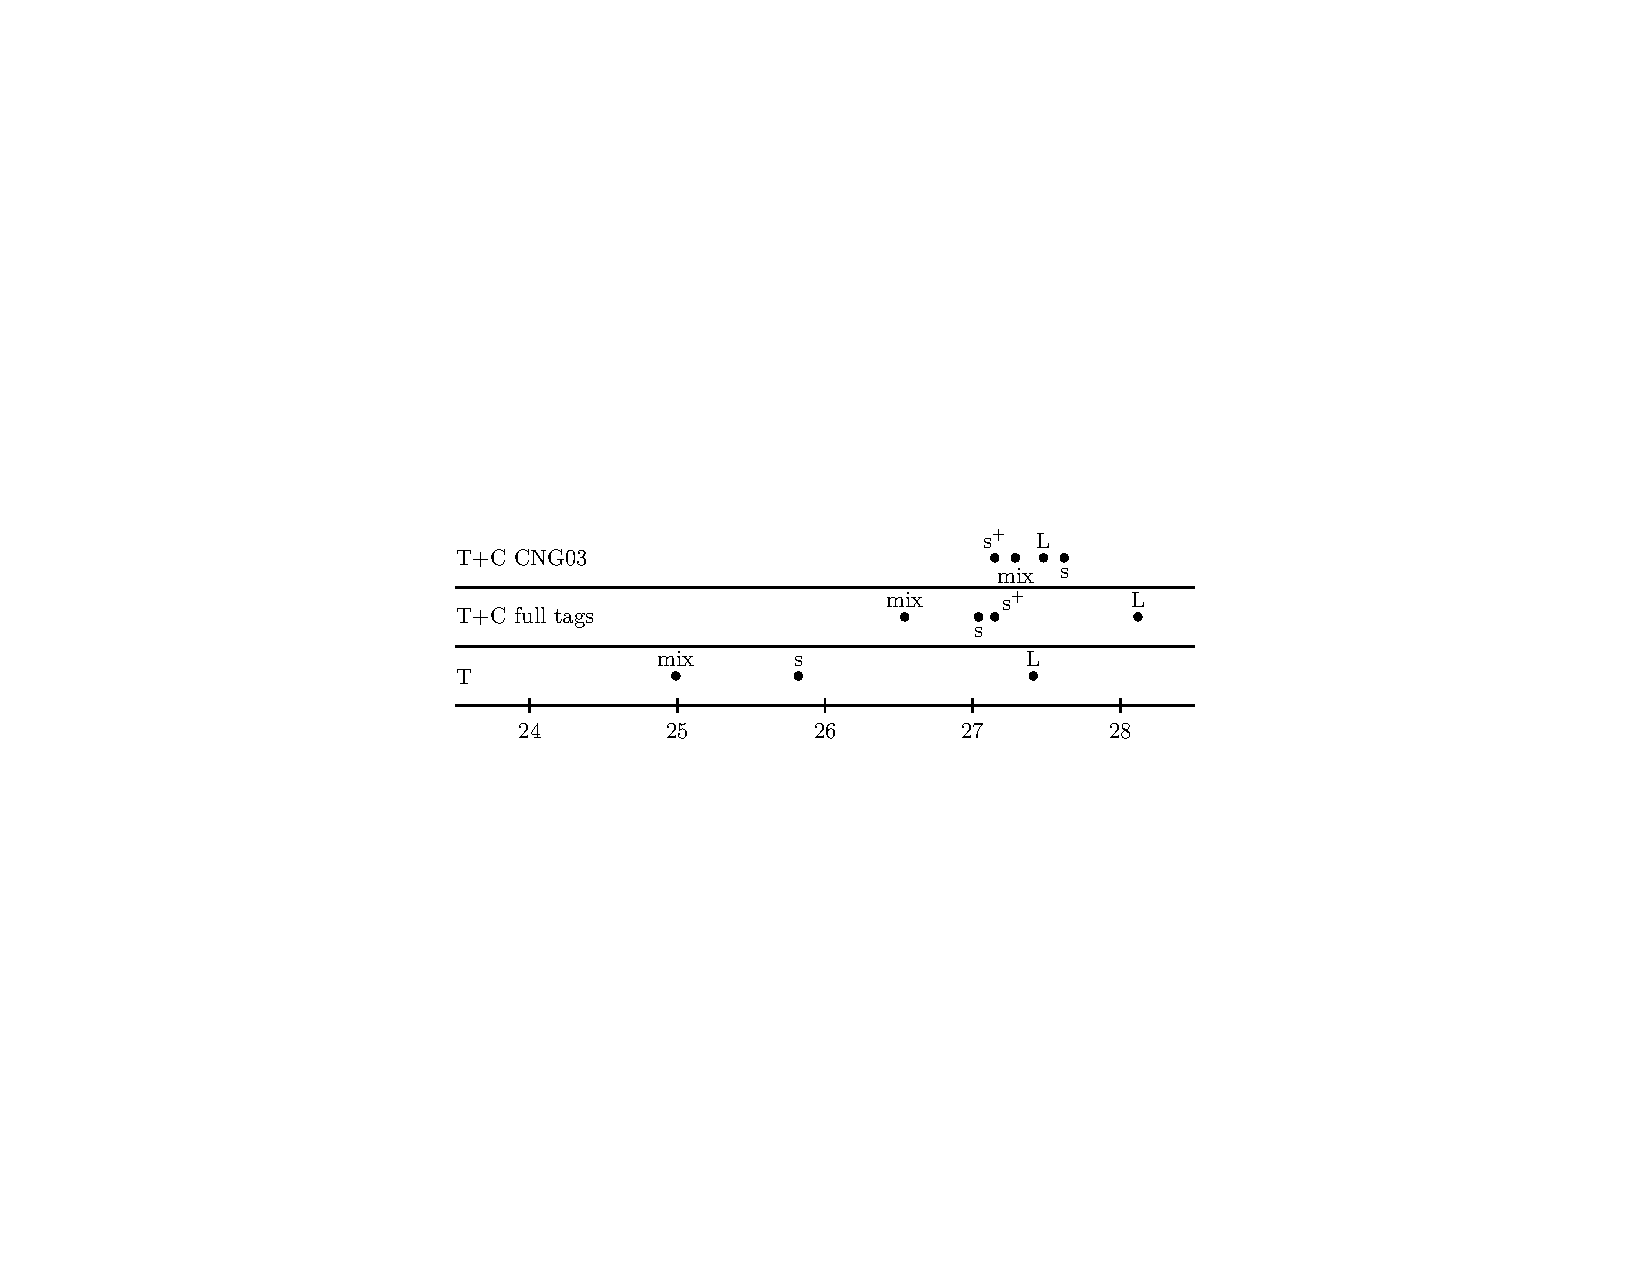
\includegraphics{images/ondrej-picture-5}
\end{center}

\begin{center}
\small
\begin{tabular}{cp{0.85\textwidth}}
s  &  small data, 20k sentences in the domain\\
s$^+$  &  small data, 20k sentences in the domain with an additional separate LM (860k sents out of the domain)\\
L  &  large data, 860k sentences, separate in-domain and out-of-domain LMs\\
mix  &  large data, 860k sentences, a single LM mixes the domains\\
\end{tabular}
\end{center}
%\begin{center}
\footnotesize
\begin{tabular}{lcccrrr}
Scenario  &  Acronym  &  Parallel Corpus  &  Language Models  &  Dev (std)  &  Dev (opt)  &  Test (opt)\\
\hline
T              &  mix    &  Large (860k)    &  Large (860k)    &  23.47  &  28.74  &        24.99\\
T              &  s      &  Baseline (20k)  &  Baseline (20k)  &  26.52  &  28.77  &        25.82\\
T+C full tags  &  mix    &  Large (860k)    &  Large (860k)    &  15.66  &  29.50  &        26.54\\
T+C full tags  &  s      &  Baseline (20k)  &  Baseline (20k)  &  22.56  &  29.65  &        27.04\\
T+C full tags  &  s$^+$  &  Baseline (20k)  &  20k+860k        &  19.97  &  30.33  &        27.15\\
T+C CNG03      &  s$^+$  &  Baseline (20k)  &  20k+860k        &  19.95  &  30.48  &        27.15\\
T+C CNG03      &  mix    &  Large (860k)    &  Large (860k)    &  15.77  &  30.71  &        27.29\\
T              &  L      &  Large (860k)    &  20k+860k        &  19.45  &  29.42  &        27.41\\
T+C CNG03      &  L      &  Large (860k)    &  20k+860k        &  14.22  &  30.33  &        27.48\\
T+C CNG03      &  s      &  Baseline (20k)  &  Baseline (20k)  &  23.27  &  30.75  &        27.62\\
T+C full tags  &  L      &  Large (860k)    &  20k+860k        &  14.06  &  30.64  &  \max{28.12}\\
\end{tabular}
%\end{center}
\caption{The effect of additional data in T and T+C scenarios.}
\label{moredatachart}
\end{figure}


Figure \ref{moredatachart} gives a chart and full details on our experiments
with adding more data into the T and T+C scenarios. We varied the scenario (T or
T+C), the level of detail in the T+C scenario (full tags vs. CNG03), the size of the
parallel corpus used to extract phrases (Baseline vs. Large, as described in
section \ref{baselinelargecorpus}) and the size or combination of target side language models (a
single LM based on the Baseline or Large corpus, or both of them with separate
weights set in the MERT training).

Several observations can be made:

\begin{itemize}

\item Ignoring the domain difference and using only the single Large language model
  (denoted \equo{mix} in the chart) hurts. Only the \equo{T+C CNG03} scenario
  does not confirm this observation and we believe this can be attributed to
  some randomness in MERT training of \equo{T+C CNG03 s$^+$}.

\item CNG03 outperforms full tags only in small data setting, with large data
  (treating the domain difference properly), full tags are significantly better.

\item The improvement of T+C over T decreases if we use more data.
\end{itemize}




\subsection{First Experiments with Verb Frames}



\subsubsection{Microstudy: Current MT Errors}
\label{microstudy}

The previous sections described significant improvements gained on small data
sets when checking morphological agreement or adding more data (BLEU raised from
25.82\% to 27.62\% or up to 28.12\% with additional out-of-domain parallel
data). However, the best result achieved is still far below the margin of
lemmatized BLEU, as estimated in section \ref{margin}. In fact, lemmatized BLEU
of our best result is yet a bit higher (35\%), indicating that T+C 
improve not only morphology, but also word order or lexical selection issues.

We performed a microstudy on local agreement between adjectives and their
governing nouns. Altogether 74\% of adjectives agreed with the governing noun
and only 2\% of adjectives did not agree; the full listing is given in Table
\ref{agreement}.

\begin{table}[t]
\begin{center}
\begin{tabular}{lr}
\bf An adjective in MT output\dots  &  \llap{\bf Portion}\\
\hline
\bf agrees with the governing noun  &  \bf 74\%\\
depends on a verb (cannot check the agreement)  &  7\%\\
misses the governing noun (cannot check the agreement)  &  7\%\\
should not occur in MT output  &  5\%\\
has the governing noun not translated (cannot check the agreement)  &  5\%\\
\bf mismatches with the governing noun  &  \bf 2\%\\
\end{tabular}
\end{center}
\caption{Microstudy: adjectives in \tocs{} MT output.}
\label{agreement}
\end{table}


Local agreement thus seems to be relatively correct. In order to find the source
of the remaining morphological errors, we performed another microstudy of
current best MT output (BLEU 28.12\%) using an intuitive metric. We checked
whether Verb-Modifier relations are properly preserved during the translation of
15 sample sentences.


%Verb:   
%ok      43 (55.8 %)
%miss    21 (27.3 %)
%bad     11 (14.3 %)
%semi    2 (2.6 %)
%Celkem  77 (100.0 %)
%
%Noun    
%ok      61 (79.2 %)
%bad     9 (11.7 %)
%unk     4 (5.2 %)
%semi    2 (2.6 %)
%miss    1 (1.3 %)
%Celkem  77 (100.0 %)


The {\it source} text of the sample sentences contained 77
Verb-Modifier pairs. Table \ref{verbmod} lists our observations on the two
members in each Verb-Modifier pair. We see that only 43\% of verbs are
translated correctly and 79\% of nouns are translated correctly. The system
tends to skip verbs quite often (21\% of cases).

\begin{table}[t]
\begin{center}
\begin{tabular}{lcc}
\bf Translation of            &  \bf Verb  &  \bf Modifier\\
\hline
\dots{}preserves meaning  &  56\%  &  79\%\\
\dots{}is disrupted       &  14\%  &  12\%\\
\dots{}is missing         &  27\%  &  1\%\\
\dots{}is unknown (not translated)         &  0\%   &  5\%\\
\end{tabular}
\end{center}
\caption{Analysis of 77 Verb-Modifier pairs in 15 sample sentences.}
\label{verbmod}
\end{table}


More
importantly, our analysis has shown that even in cases where both the Verb and
the Modifier are correct, the relation between them in Czech is either
non-gramatical or meaning-disturbing in 56\% of these cases. Commented samples
of such errors are given in Figure \ref{sampleerrors}. The first sample shows
that a strong language model can lead to the choice of a grammatical relation
that nevertheless does not convey the original meaning. The second sample
illustrates a situation where two correct options are available but the
system chooses an inappropriate relation, most probably because of backing off to
a generic pattern verb-noun$_{plural}^{accusative}$. This pattern
is quite common for
for expressing the object role of
many verbs (such as \text{vydat}, see Correct
option 2 in Figure \ref{sampleerrors}), but does not fit well with the verb
\text{vyb\v{e}hnout}. While the target-side data
may be rich enough to learn the generalization vyb\v{e}hnout--s--{\it instr},
no
such generalization is possible with language models over word forms or
morphological tags only. The
target side data will be hardly ever rich enough to learn this particular
structure in all correct morphological and lexical variants:
\text{vyb\v{e}hl--s--reklamou, vyb\v{e}hla--s--reklamami,
vyb\v{e}hl--s--prohl\'{a}\v{s}en\'{\i}m, vyb\v{e}hli--s--ozn\'{a}men\'{\i}m,
\dots}. We would need a 
mixed
model that combines verb lemmas, prepositions and case information to properly
capture the relations.


\begin{figure}

\begin{center}
{\small
\begin{tabular}{|ll|}
\hline
Input:      &  {Keep on investing.}\\
MT output:  &  Pokra\v{c}ovalo investov\'{a}n\'{\i}. (grammar correct here!)\\
Gloss:      &  Continued investing. (Meaning: The investing continued.)\\
Correct:    &  {Pokra\v{c}ujte v investov\'{a}n\'{\i}.}\\
\hline
\end{tabular}
}
\end{center}


\begin{center}
{
\small
\begin{tabular}{|lllll|}
\hline
Input:  &  \multicolumn{4}{l|}{brokerage firms rushed out ads \dots}\\
MT Output:  &  brokersk\'{e}  &  firmy  &  vyb\v{e}hl  &  reklamy\\
Gloss:  &  brokerage  &  firms$_{pl.fem}$  &  ran$_{sg.masc}$  &  ads$_{pl.nom,pl.acc}^{pl.voc,sg.gen}$\\
Correct option 1:  &  brokersk\'{e}  &  firmy  &  vyb\v{e}hly  &  s reklamami$_{pl.instr}$\\
Correct option 2:  &  brokersk\'{e}  &  firmy  &  vydaly  &  reklamy$_{pl.acc}$\\
\hline
\end{tabular}
}
\end{center}
\caption{Two sample errors in translating Verb-Modifier relation from English to
Czech.}
\label{sampleerrors}
\end{figure}







To sum up, the analysis has revealed that in our best MT output:

\begin{itemize}

\item noun-adjective agreement is already quite fine,

\item verbs are often missing,

\item verb-modifier relations are often malformed.
\end{itemize}


\subsubsection{Design of Verb Frame Factor}


In this section we describe a model that combines verb lemmas, prepositions and
noun cases to improve the verb-modifier relations on the target side and
possibly to favour keeping verbs in MT output. The model
is incorporated to our MT system in the most simple fashion: we simply create an
additional output factor to explicitly model target verb
valency/subcategorization, i.e. to mark verbs and their modifiers in the output.
An independent language model is used to ensure coherence in the verb frame
factor.

Figure \ref{samplevf} illustrates the process of converting a Czech sentence to
the corresponding verb frame factor. We make use of the dependency analysis of
the sentence and associate each input word with a token:

\begin{itemize}

\item tokens for verbs have the form \text{H:V\ang{subpart of speech}:\ang{verb
  lemma}} indicating that the verb is the head of the frame,

\item tokens for words depending on a verb have the form \text{M:\ang{slot
  description}} to denote verb frame members. Slot description is based on the
  respective modifier:
\begin{itemize}

\item slot description for nouns, pronouns and (nominalized) adjectives contains
  only the case information (e.g. \text{subst$_{nom}$} for nouns or pronouns in
  nominative),

\item slot description for prepositions contains the preposition lemma and the
  case (e.g. \text{prep:na$_{acc}$} for the preposition \text{na} in accusative),

\item sub-ordinating conjunctions are represented by their lemma (e.g.
  \text{subord:zda} for the conjunction \text{zda}),

\item co-ordinating conjunctions are treated in an oversimplified manner, the slot
  description just notes that there was a co-ordinating conjunction. No
  information is propagated from the co-ordinated elements.

\item adverbs are completely ignored, i.e. get a dummy token \text{---}
\end{itemize}

\item punctuation symbols have the form \text{PUNCT:\ang{punctuation symbol}} and
  conjunctions have the form \text{DELIM:\ang{subpart of
  speech}:\ang{conjunction lemma}} to
  keep track of structural delimiters in the verb frame factor,

\item all other words get a dummy token \text{---}.
\end{itemize}

Thus for the beginning of the sample sentence in Figure \ref{samplevf}
\text{Popt\'{a}vka trvale stoup\'{a} za podpory\dots (The demand has been consistently
growing under the encouragement\dots)} we create the following stream:

\begin{center}
M:subst$_{nom}$ --- H:VB:stoupat M:prep:za$_{gen}$ ---
\end{center}

The stream indicates that the verb \text{stoupat} tends to be modified by a
(preceding) subject and (following) argument or adjunct governed by the
preposition \text{za} in genitive.

Keeping in mind the valency theory for Czech (e.g. \perscite{panevova:94}),
there are several limitations in our model:

\begin{itemize}

\item We do not make any distinctions between
argument and adjuncts (except for the above mentioned deletion of adverbs).
Ideally, all adjuncts would get the dummy token \text{---}.


\item In theory,
the order of verb frame members is not grammatically significant for some
languages, so we should allow independent reordering of the verb frame factor.


\item If a verb depends on a verb, their modifiers can be nearly arbitrarily mixed
  within the clause (in Czech). Our model does not distinguish which modifiers
  belong to which of the verbs.

\end{itemize}

Another problem with the verb frame factor is the explicit representation of
the number of intervening words (tokens \text{---}). A skipping language model
would be necessary to describe the linguistic reality more adequately.


%<s id="wsj-underscore-1200.cz:3">
%<f>Popt\'{a}vka<MDl src="a">popt\'{a}vka<MDt src="a">NNFS1-----A----<A>Sb<r>1<g>3
%<f>trvale<MDl src="a">trvale-underscore--caret--underscore-*1\'{y}-underscore-<MDt src="a">Dg-------1A----<A>Adv<r>2<g>3
%<f>stoup\'{a}<MDl src="a">stoupat-underscore-:T<MDt src="a">VB-S---3P-AA---<A>Obj<r>3<g>9
%<f>za<MDl src="a">za-1<MDt src="a">RR--2----------<A>AuxP<r>4<g>3
%<f>podpory<MDl src="a">podpora-underscore--caret--underscore-pen\'{\i}ze;-underscore-ty\v{c};-underscore-mor\'{a}ln\'{\i}-underscore-p.-underscore-<MDt src="a">NNFS2-----A----<A>Adv<r>5<g>4
%<f>vl\'{a}dn\'{\i}<MDl src="a">vl\'{a}dn\'{\i}<MDt src="a">AAFS2----1A----<A>Atr<r>6<g>7
%<f>politiky<MDl src="a">politika-underscore--caret--underscore-v\v{e}da-underscore-<MDt src="a">NNFS2-----A----<A>Atr<r>7<g>5
%<f>,<MDl src="a">,<MDt src="a">Z:-------------<A>AuxX<r>8<g>3
%<f>\v{r}ekl<MDl src="a">\v{r}\'{\i}ci<MDt src="a">VpYS---XR-AA---<A>Pred<r>9<g>0
%<f>mluv\v{c}\'{\i}<MDl src="a">mluv\v{c}\'{\i}<MDt src="a">NNMS1-----A----<A>Sb<r>10<g>9

%popt\'{a}vka trvale stoup\'{a} za podpory prospot\v{r}ebitelsk\'{e} vl\'{a}dn\'{\i} politiky , \v{r}ekl mluv\v{c}\'{\i} asociace .
%MEMBER:subst+1 --- HEAD:VB:stoupat_:T MEMBER:Rza-1+2 --- --- --- --- MEMBER:Z- HEAD:Vp:\v{r}\'{\i}ci MEMBER:subst+1 --- PUNCT:.

%<f>\broken{Popt\'{a}vka\\MEMBER:subst+1}<A>Sb<r>1<g>3
%<f>\broken{trvale\\---}<A>Adv<r>2<g>3
%<f>\broken{stoup\'{a}\\HEAD:VB:stoupat\_:T}<A>Obj<r>3<g>9
%<f>\broken{za\\MEMBER:Rza-1+2}<A>AuxP<r>4<g>3
%<f>\broken{podpory\\---}<A>Adv<r>5<g>4
%<f>\broken{vl\'{a}dn\'{\i}\\---}<A>Atr<r>6<g>7
%<f>\broken{politiky\\---}<A>Atr<r>7<g>5
%<f>\broken{,\\MEMBER:Z-}<A>AuxX<r>8<g>3
%<f>\broken{\v{r}ekl\\HEAD:Vp:\v{r}\'{\i}ci}<A>Pred<r>9<g>0
%<f>\broken{mluv\v{c}\'{\i}\\MEMBER:subst+1}<A>Sb<r>10<g>9
%<f>\broken{.\\PUNCT:.}<A>AuxK<r>11<g>0

\begin{figure}[ht]
\begin{center}
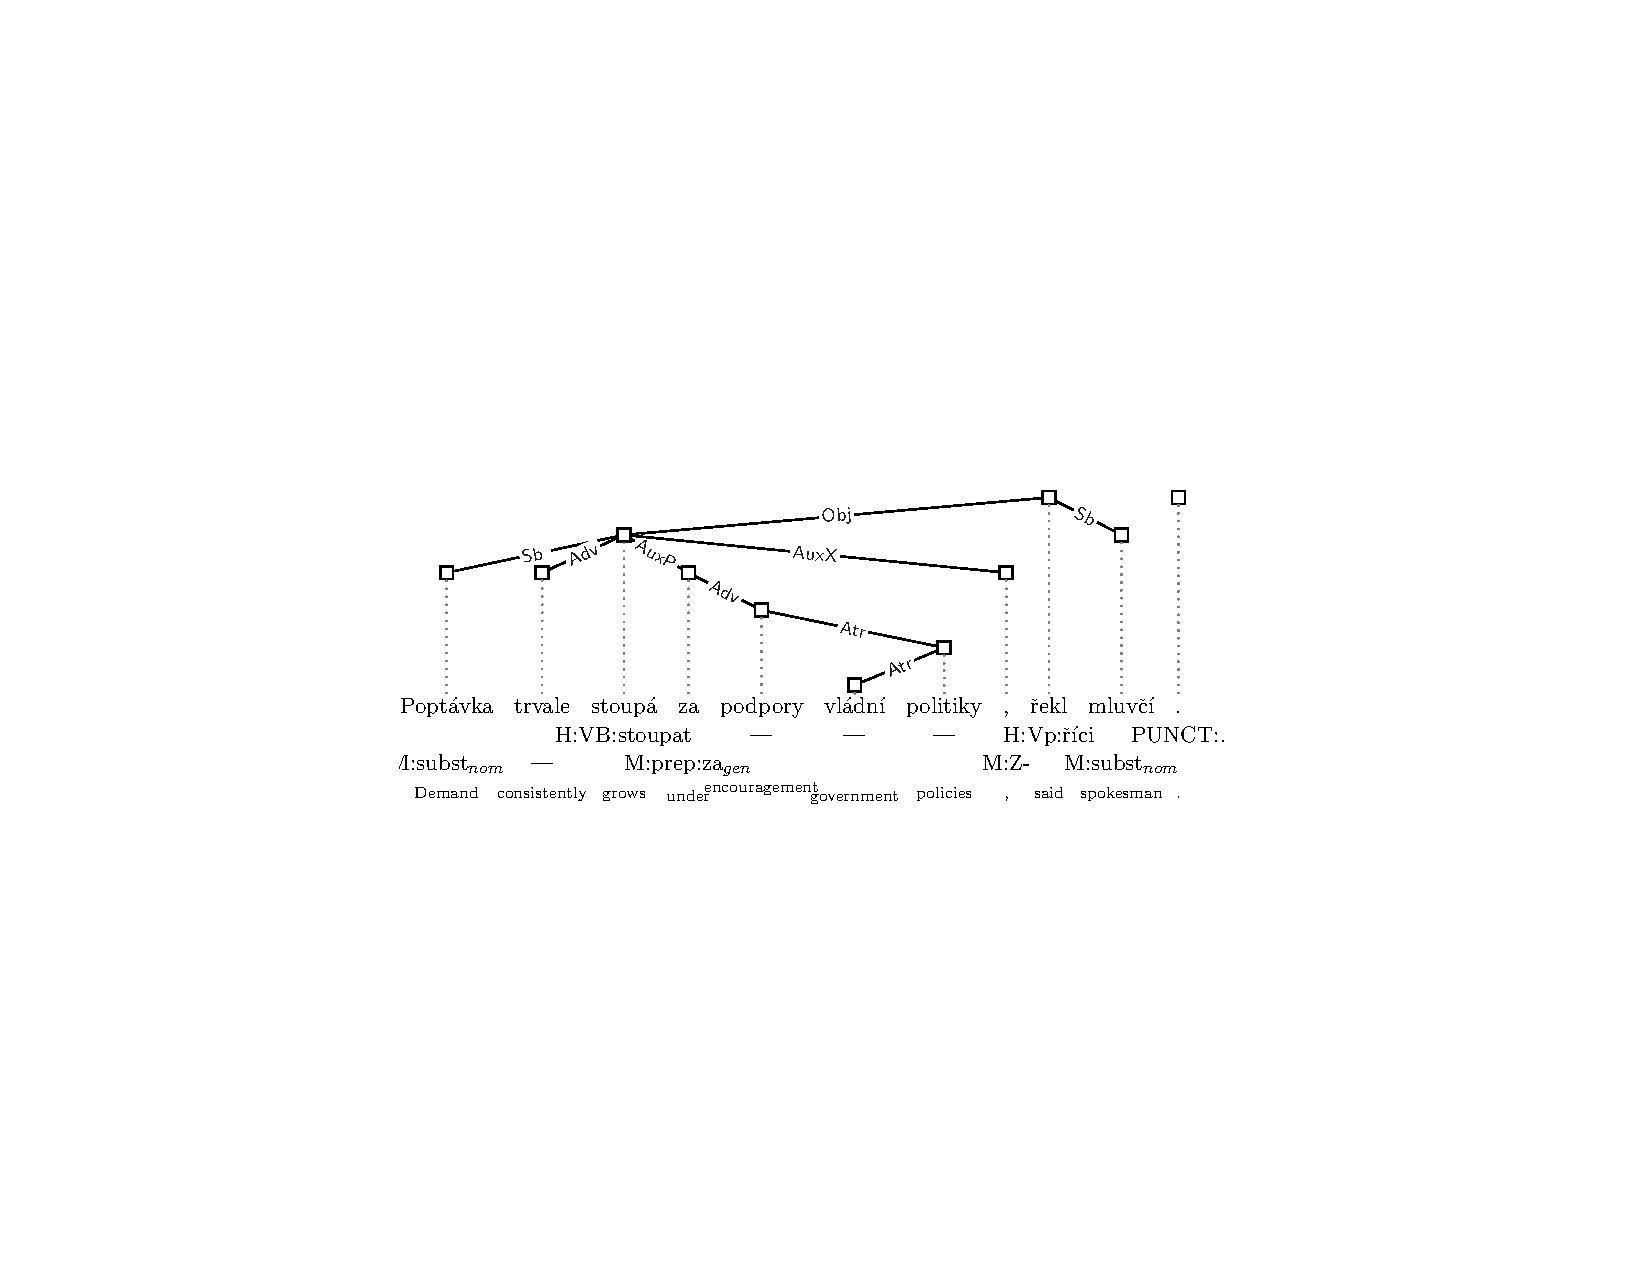
\includegraphics{images/ondrej-picture-6}
\end{center}
\caption{Verb frame factor based on dependency syntax tree of a sample sentence:
\text{
Demand has been growing consistently under the encouragement of government policies, a spokesman said.
}}
\label{samplevf}
\end{figure}

%Popt\'{a}vka   	Sb  	 1	3	popt\'{a}vka	MEMBER:subst+1
%trvale         	Adv 	 2	3	trvale  	---
%stoup\'{a}     	Obj 	 3	9	stoup\'{a}  	HEAD:VB:stoupat\_:T
%za             	AuxP	 4	3	za      	MEMBER:Rza-1+2
%podpory        	Adv 	 5	4	podpory 	---
%vl\'{a}dn\'{\i}	Atr 	 6	7	vl\'{a}dn\'{\i}  	---
%politiky       	Atr 	 7	5	politiky	---
%,              	AuxX	 8	3	,       	MEMBER:Z-
%\v{r}ekl       	Pred	 9	0	\v{r}ekl    	HEAD:Vp:\v{r}\'{\i}ci
%mluv\v{c}\'{\i}	Sb  	10	9	mluv\v{c}\'{\i}  	MEMBER:subst+1
%.              	AuxK	11	0	.       	PUNCT:.

%<s id="wsj-underscore-1200.mrg:3">
%<f>Demand<l>demand<t>NN<A>Sb<r>1<g>4<x name="Wf">-SBJ<x name="Wl">NP~-SBJ<x name="wsj-underscore-id">wsj-underscore-1200.mrg:3/1<x name="wsj-underscore-id2">wsj-underscore-1200.mrg:3/1
%<f>has<l>have<t>VBZ<A>AuxV<r>2<g>4<x name="wsj-underscore-id">wsj-underscore-1200.mrg:3/3<x name="wsj-underscore-id2">wsj-underscore-1200.mrg:3/2
%<f>been<l>be<t>VBN<A>Atr<r>3<g>4<x name="wsj-underscore-id">wsj-underscore-1200.mrg:3/4<x name="wsj-underscore-id2">wsj-underscore-1200.mrg:3/3
%<f>growing<l>grow<t>VBG<A>Obj<r>4<g>17<x name="Wf">-TPC-1<x name="Wl">S~-TPC-1<x name="wsj-underscore-id">wsj-underscore-1200.mrg:3/5<x name="wsj-underscore-id2">wsj-underscore-1200.mrg:3/4
%<f>consistently<l>consistently<t>RB<A>Adv<r>5<g>4<x name="Wf">-MNR<x name="Wl">ADVP-MNR<x name="wsj-underscore-id">wsj-underscore-1200.mrg:3/6<x name="wsj-underscore-id2">wsj-underscore-1200.mrg:3/5
%<f>under<l>under<t>IN<A>AuxP<r>6<g>4<x name="Wf">-LOC<x name="Wl">PP-LOC<x name="wsj-underscore-id">wsj-underscore-1200.mrg:3/8<x name="wsj-underscore-id2">wsj-underscore-1200.mrg:3/6
%<f>the<l>the<t>DT<A>Atr<r>7<g>8<x name="wsj-underscore-id">wsj-underscore-1200.mrg:3/9<x name="wsj-underscore-id2">wsj-underscore-1200.mrg:3/7
%<f>encouragement<l>encouragement<t>NN<A>Adv<r>8<g>6<x name="Wl">NP~<x name="wsj-underscore-id">wsj-underscore-1200.mrg:3/10<x name="wsj-underscore-id2">wsj-underscore-1200.mrg:3/8
%<f>of<l>of<t>IN<A>AuxP<r>9<g>8<x name="Wl">PP<x name="wsj-underscore-id">wsj-underscore-1200.mrg:3/12<x name="wsj-underscore-id2">wsj-underscore-1200.mrg:3/9
%<f>pro-consumption<l>pro-consumption<t>NN<A>Atr<r>10<g>12<x name="wsj-underscore-id">wsj-underscore-1200.mrg:3/13<x name="wsj-underscore-id2">wsj-underscore-1200.mrg:3/10
%<f>government<l>government<t>NN<A>Atr<r>11<g>12<x name="wsj-underscore-id">wsj-underscore-1200.mrg:3/14<x name="wsj-underscore-id2">wsj-underscore-1200.mrg:3/11
%<f>policies<l>policy<t>NNS<A>Atr<r>12<g>9<x name="Wl">NP~<x name="wsj-underscore-id">wsj-underscore-1200.mrg:3/15<x name="wsj-underscore-id2">wsj-underscore-1200.mrg:3/12
%<D>
%<d>,<l>,<t>,<A>AuxX<r>13<g>17<x name="wsj-underscore-id">wsj-underscore-1200.mrg:3/24<x name="wsj-underscore-id2">wsj-underscore-1200.mrg:3/13
%<f>an<l>an<t>DT<A>Atr<r>14<g>16<x name="wsj-underscore-id">wsj-underscore-1200.mrg:3/25<x name="wsj-underscore-id2">wsj-underscore-1200.mrg:3/14
%<f>association<l>association<t>NN<A>Atr<r>15<g>16<x name="wsj-underscore-id">wsj-underscore-1200.mrg:3/26<x name="wsj-underscore-id2">wsj-underscore-1200.mrg:3/15
%<f>spokesman<l>spokesman<t>NN<A>Sb<r>16<g>17<x name="Wf">-SBJ<x name="Wl">NP~-SBJ<x name="wsj-underscore-id">wsj-underscore-1200.mrg:3/27<x name="wsj-underscore-id2">wsj-underscore-1200.mrg:3/16
%<f>said<l>say<t>VBD<A>Pred<r>17<g>0<x name="Wl">S<x name="wsj-underscore-id">wsj-underscore-1200.mrg:3/29<x name="wsj-underscore-id2">wsj-underscore-1200.mrg:3/17
%<D>
%<d>.<l>.<t>.<A>AuxK<r>18<g>0<x name="wsj-underscore-id">wsj-underscore-1200.mrg:3/35<x name="wsj-underscore-id2">wsj-underscore-1200.mrg:3/18


\subsubsection{Preliminary Results with Verb Frame Factor}

Table \ref{vfresults} displays BLEU scores of the scenario translate-and-check verb factor
(T+Cvf) compared to the single-factored baseline (T). Word alignment for these
experiments was obtained using grow-diag-final heuristic on stemmed English and
lemmatized Czech texts. Only the baseline corpus (20k sentences) was used to
extract phrase tables. The verb frame factor language model is a simple $n$-gram
LM with $n$ of 7, 9 or 11 and it is based either on the baseline corpus (PCEDT)
or the Czech side of the Large corpus. In all cases, a simple trigram model
checks the fluency of word form stream.


%VFF: vf LM1-11-czeng	28.68      	19.51       	24.23
%Baseline: t0-0       	29.24*      	25.68>      	25.23>

\begin{table}[ht]
\begin{center}
\begin{tabular}{lccc}
                       &  Dev (std)  &  Dev (opt)  &  Test (opt)\\
\hline
T+Cvf LM-11gr-Large    &         19.51  &       28.68  &        24.23\\
T+Cvf LM-7gr-Baseline  &         19.75  &       28.54  &        25.05\\
T+Cvf LM-7gr-Large     &         19.69  &       28.32  &        25.07\\
T+Cvf LM-9gr-Large     &         19.55  &       27.98  &        25.09\\
Baseline: T            &         25.68  &       29.24  &  \max{25.23}\\
\end{tabular}
\end{center}
\caption{Preliminary results with checking of verb frame factor.}
\label{vfresults}
\end{table}

Unfortunately, all T+Cvf results fall below the single-factored baseline.
Table \ref{vffanalysis} gives some more detail on this result. We performed the
same type of analysis of verb-modifier pairs in the first 15 output sentences,
as described in section \ref{microstudy}. The baseline columns are based on the
single-factored output (BLEU 25.23), the VFF columns are based on T+Cvf
LM-11gr-Large (BLEU 24.23).


\begin{table}[ht]
\begin{center}
\begin{tabular}{lcc|cc}
\bf Translation of  &  \multicolumn{2}{c}{\bf Verb}  &  \multicolumn{2}{c}{\bf Modifier}\\
      &  Baseline  &  VFF  &  Baseline  &  VFF\\
\hline
\dots{}preserves meaning    &     38  &    40  &     57  &    55\\
\dots{}is disrupted   &     17  &    20  &     15  &    15\\
\dots{}is missing  &     15  &    10  &      0  &     1\\
\dots{}is unknown (not translated)   &      7  &     7  &      5  &     6\\
\end{tabular}
\end{center}
\caption{Analysis of 77 Verb-Modifier pairs in baseline output and in
verb-frame-factor (VFF) output.}
\label{vffanalysis}
\end{table}

Despite the very small size of our sample, some effects
of adding the verb-frame-factor can be observed. On the positive side, verbs are
not missing in MT output that often. On the negative side, translation of verbs
or nouns gets confused by the additional factor. Unfortunately, also the
percentage of correctly translated verb-modifier relations in cases where both
verb and modifier are fine decreased.

Unless the experiment is repeated with more training data and also with a larger
set of evaluated sentences, it is hard to make any conclusions. The
verb frame factor at least leads to some more verbs in MT output.


%VFF
%Rok	18 (58.1 %)
%Rbad	13 (41.9 %)
%Celkem	31 (100.0 %)


% BASE
%Rok	19 (63.3 %)
%Rbad	11 (36.7 %)
%Celkem	30 (100.0 %)




\subsection{Single-factored Results \toen{}}

Our primary interest was in \tocs{} translation but we also experimented with
\toen{} direction, mainly to allow for comparison with previous reported
results.

It should be noted that translating to English in our setting is easier. In
general, there are fewer word forms in English so language models face milder
data spareness and there are fewer chances to make an error (BLEU would notice).
Moreover, the particular test set we use contains input Czech text that came
from an English original and was translated sentence by sentence.  The Czech
thus probably does not exhibit full richness and complexity of word order and
language constructions and is easier to translate back to English than a generic
Czech text would be.


\begin{table}[ht]
\begin{center}
\small
\begin{tabular}{lccccc}
Scenario  &  Parallel Corpus  &  Language Models                &  Dev (std)  &  Dev (opt)  &  Test (opt)\\
\hline
T         &  Baseline (20k)   &  Baseline (20k)                 &      28.97  &      35.39  &        28.50\\
T+C       &  Baseline (20k)   &  Baseline (20k)                 &      23.07  &      36.13  &        28.66\\
T         &  Large (860k)     &  20k+860k                       &      19.31  &      39.60  &        33.37\\
T         &  Large (860k)     &  \clap{Large (860k, i.e. mix)}  &      28.94  &      40.15  &  \max{34.12}\\
\end{tabular}
\end{center}
\caption{Sample \toen{} BLEU scores.}
\label{english}
\end{table}

Table \ref{english} lists Moses results of \toen{} translation. We observe a
minor improvement when checking the part-of-speech factor (T+C). A larger
improvement is obtained
by adding more data and quite differently from \tocs{} results (see section
\ref{moredata}), mixing in-domain
and out-of-domain LM data does not hurt the performance.


\subsection{Summary and Conclusion}

We experimented with factored \tocs{} translation. The majority of our
experiments were carried out in a small data setting and we translated to a
morphologically rich language. In this setting, lemmatization or stemming of
training data is vital for obtaining reliable alignments. Multi-factored
translation for ensuring coherence of morphological properties of output words
significantly increases BLEU performance, although the effect is reduced with
additional training data. Experiments also indicate that more complex
translation scenarios lower the scores, probably due to more severe search
errors.

Our \tocs{} experiments confirm that in minimum-error-rate training, it is
helpful to keep language models based on in- and out-of-domain data separate. We
did not observe this domain sensitivity in \toen{} direction.

Based on manual analysis of sample output sentences, we also conducted some
preliminary experiments on using target-side syntactic information in order to
improve grammaticality of verb-modifier relations.  The results are rather
inconclusive and further refinement of the model would be necessary.

}  % wrapping all Ondrej's content to prevent confusing macros





\chapter{Undergraduate Projects}

This appendix details the work undertaken by the three exceptional undergraduates who participated in the summer workshop.  Their projects focused on three different topics:
\begin{itemize}
\item  Alexandra Constantin's project focused on extending factored translation models to be used in the {\it word alignment} phrase of translation, rather than in the {\it decoding} phrase which was the general thrust of the workshop.  Her project is described in Section \ref{Alex's-project}.
\item  Christine Corbett Moran collaborated with Brooke Cowan to implement lexicalized re-ordering models in Moses.  This was one of the single largest improvements to overall translation quality which was incorporated during the workshop.  It is described in Section   \ref{Christine's-project}.
\item Evan Herbst created a set of tools for performing error analysis of machine translation output.  His project provided visualization tools for the translations of individual sentences, as well as a set of tools for summary statistics at the corpus level.  His project described in Section \ref{Evan's-project}.
\end{itemize}

\section{Linguistic Information for Word Alignment}\label{Alex's-project}
%{\sc Alexandra Constantin}

\subsection{Word Alignment}

If we open a common bilingual dictionary, we find that many words have multiple translations, some of which are more likely
than others, for instance:

\begin{center}
\textbf{Haus} = house, building, home, household
\end{center}

If we had a large collection of German text, paired with its
translation into English, we could count how often $Haus$ is
translated into each of the given choices. We can use the counts to
estimate a lexical translation probability distribution

\begin{center}
$t : e|f \rightarrow t(e|f)$
\end{center}

that, given a foreign word, $f$, returns a probability for each
choice for an English translation $e$, that indicates how likely
that translation is.


We can derive an estimate of the translation probability
distribution from the data by using the ratio of the counts. For
example, if we have $10000$ occurrences of $Haus$ and $8000$
translate to $house$, then $t(house|Haus)=0.8$.

For some words that are infrequent in the corpus, the estimates of
the probability distribution are not very accurate. Using other
linguistic information, such as observing that in a specific
language pair verbs usually get translated as verbs, could help in
building a more accurate translation.

Let's look at an example. Imagine we wanted to translate the German
sentence \textbf{\emph{das Haus ist klein}}. The sentence can be
translated word by word into English. One possible translation is
\textbf{\emph{the house is small}}.


Implicit in these translations is an alignment, a mapping from
German words to English words:

\begin{center}
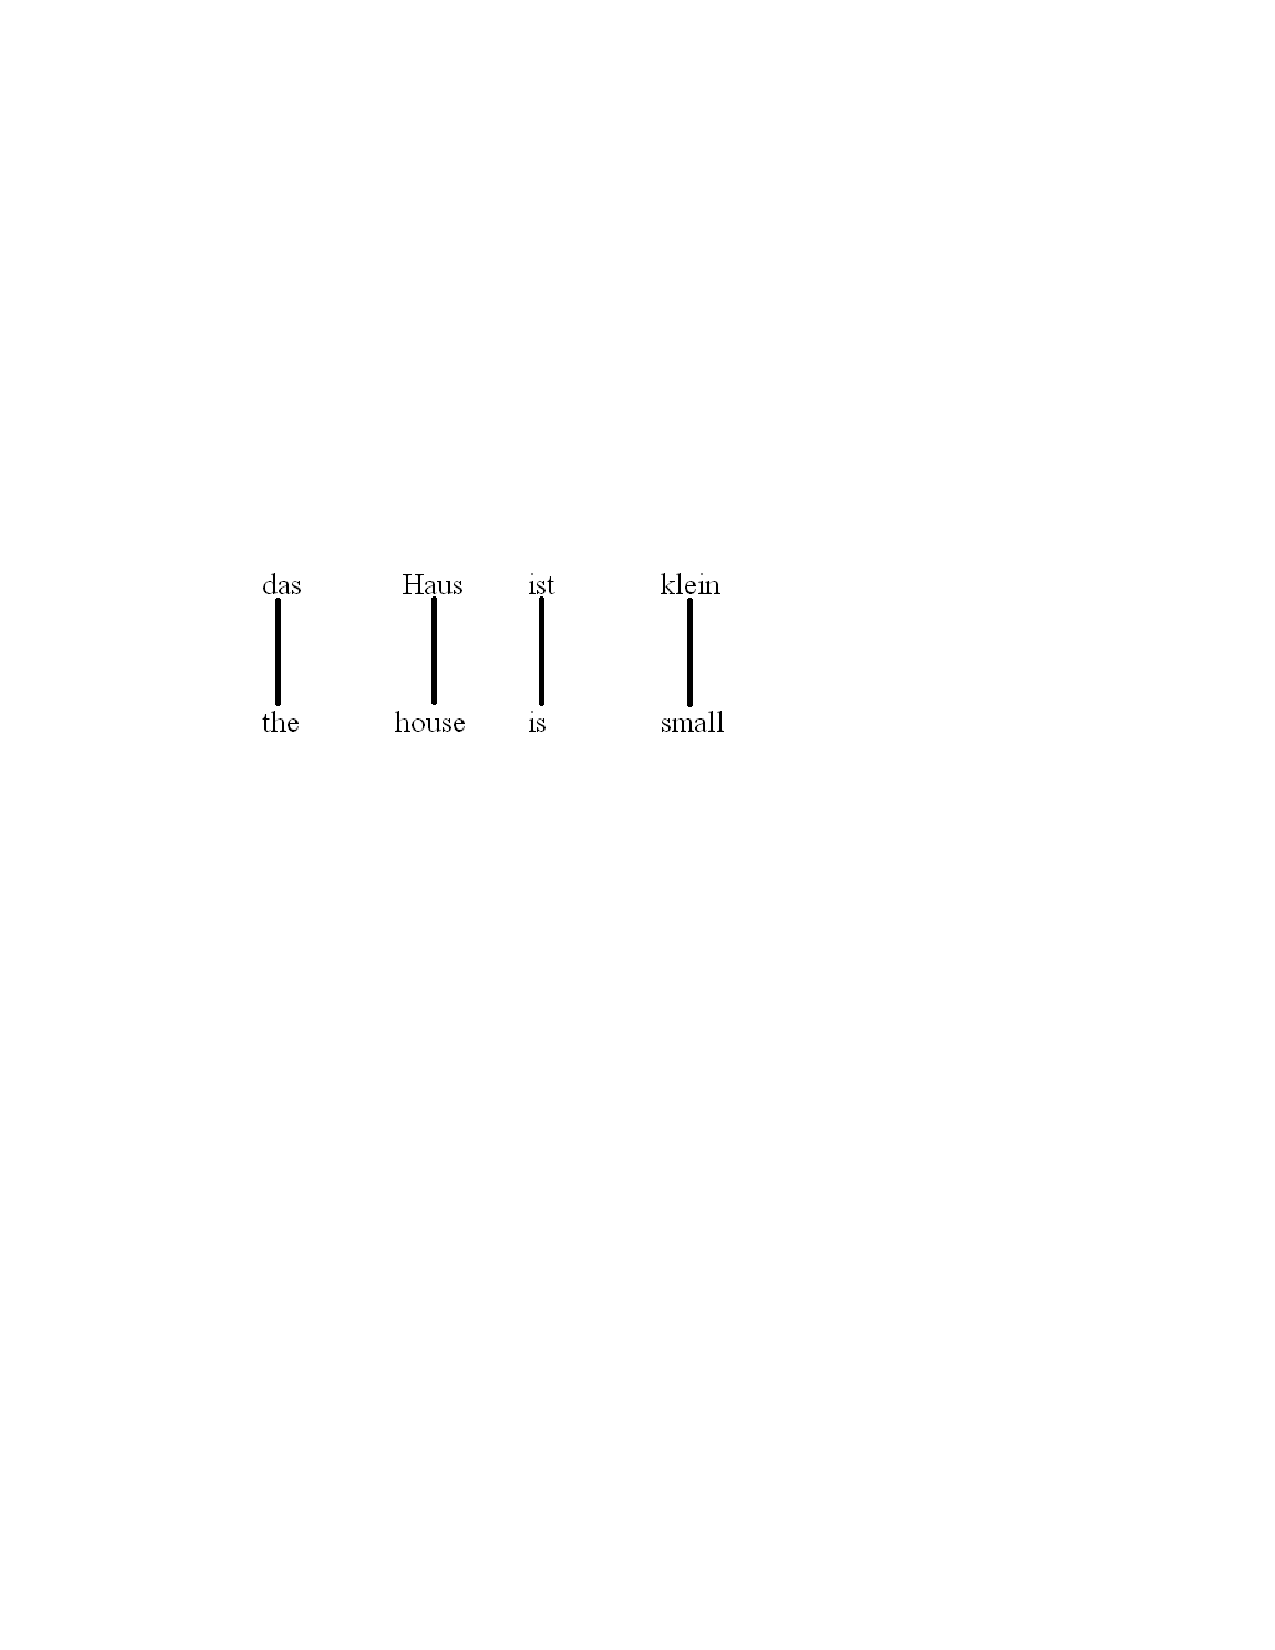
\includegraphics[viewport = 100 440 400 530,clip,scale=0.5]{constantin-figure1.pdf}
\end{center}

An alignment can be formalized with an alignment function $a : i
\rightarrow j$. This function maps each English target word at
position $i$ to a German source word at position $j$.

For example, if we are given the following pair of sentences:

\begin{center}
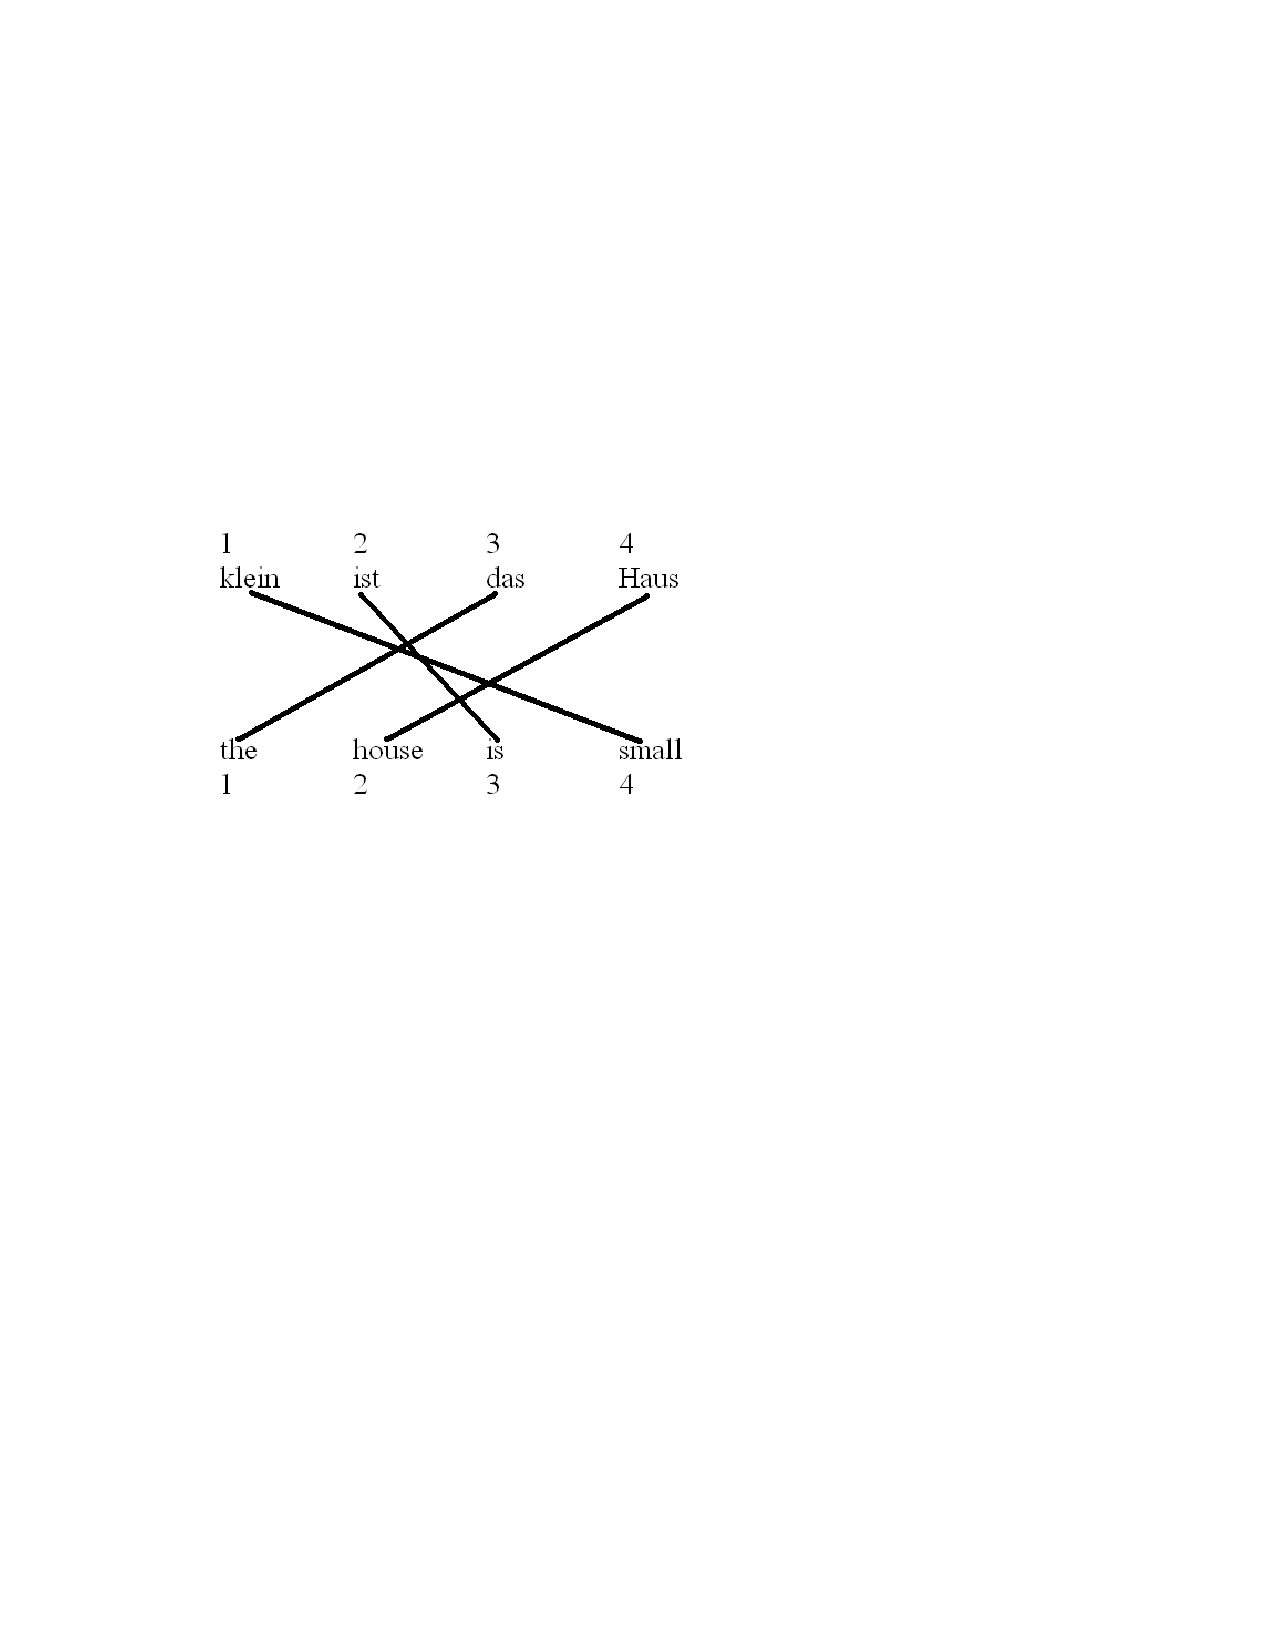
\includegraphics[viewport = 100 400 400 550,clip,scale=0.5]{constantin-figure2.pdf}
\end{center}

the alignment function will be
$a:\{1 \rightarrow 3, 2 \rightarrow 4, 3 \rightarrow 2, 4
\rightarrow 1\}$.

\subsection{IBM Model 1}

Lexical translations and the notion of alignment allow us to define
a model capable of generating a number of different translations for
a sentence, each with a different probability. One such model is IBM
Model 1, which will be described below.

For each target word $e$ that is produced by the model from a source
word $f$, we want to factor in the translation probability $t(e|f)$.

The translation probability of a foreign sentence
$\textbf{f}=(f_1,\dots,f_{l_f})$ of length $l_f$ into an English
sentence $\textbf{e}=(e_1,\dots, e_{l_e})$ of length $l_e$ with an
alignment of each English word $e_j$ to a foreign word $f_i$
according to alignment $a:j \rightarrow i$ is:

\begin{center}
$p(\textbf{e},a|\textbf{f}) = \frac{\epsilon}{(l_f +
1)^{l_e}}\prod_{j=1}^{l_e} t(e_j|f_{a(j)})$
\end{center}


\subsection{Learning the Lexical Translation Model}

A method for estimating these translation probability distributions
from sentence-aligned parallel text is now needed.

The previous section describes a strategy for estimating the lexical
translation probability distributions from a word-aligned parallel
corpus. However, while large amounts of sentence-aligned parallel
texts can be easily collected, word-aligned data cannot. We would
thus like to estimate these lexical translation distributions
without knowing the actual word alignment, which we consider a
hidden variable. To do this, we use the Expectation-Maximization
algorithm:
\vspace{-3pt}
{
\begin{itemize} \itemsep=-3pt
\item{Initialize model (typically with uniform distribution)}
\item{Apply the model to the data (expectation step)}
\item{Learn the model from the data (maximization step)}
\item{Iterate steps 2-3 until convergence}
\end{itemize}
}

First, we initialize the model. Without prior knowledge, uniform
probability distributions are a good starting point. In the
expectation step, we apply the model to the data and estimate the
most likely alignments. In the maximization step, we learn the model
from the data and augment the data with guesses for the gaps.

\subsubsection{Expectation step}

When we apply the model to the data, we need to compute the
probability of different alignments given a sentence pair in the
data:
\vspace{-1mm}
\begin{center}
$p(a|\textbf{e},\textbf{f}) =
\frac{p(\textbf{e},a|\textbf{f})}{p(\textbf{e}|\textbf{f})}$
\end{center}

$p(\textbf{e}|\textbf{f})$, the probability of translating sentence
$\textbf{f}$ into sentence $\textbf{e}$ is derived as:
\vspace{-1mm}
\begin{center}
$p(\textbf{e}|\textbf{f}) = \sum_a p(\textbf{e},a|\textbf{f}) =
\prod_{j=1}^{l_e} \sum_{i=0}^{l_f}t(e_j|f_i)$
\end{center}

Putting the previous two equations together,
\vspace{-1mm}
\begin{center}
 $p(a|\textbf{e},\textbf{f}) =
\frac{p(\textbf{e},a|\textbf{f})}{p(\textbf{e}|\textbf{f})}
=\prod_{j=1}^{l_e} \frac {t(e_j | f_{a(j)})}{\sum_{i=0}^{l_f}
t(e_j|f_i)}$.
\end{center}

\subsubsection{Maximization Step}

For the maximization step, we need to collect counts over all
possible alignments, weighted by their probabilities. For this
purpose, we define a count function $c$ that collects evidence from
a sentence pair $(\textbf{e},\textbf{f})$ that a particular source
word $f$  translates into a particular target word $e$.

\begin{center}

$c(e|f;\textbf{e},\textbf{f}) = \sum_a p(a|\textbf{e},\textbf{f}) =
\frac{t(e|f)}{\sum_{j=1}^{l_e}t(e|f_{a(j)})} \sum_{j=1}^{l_e}
\delta(e,e_j)\sum_{i=0}^{l_f}\delta(f,f_i)$

\end{center}

where $\delta(x,y)$ is $1$ is $x=y$ and $0$ otherwise.

Given the count function, we can estimate the new translation
probability distribution by:

\begin{center}
$t(e|f;\textbf{e},\textbf{f}) =
\frac{\sum_{(\textbf{e},\textbf{f})}c(e|f;\textbf{e},\textbf{f})}{\sum_f\sum_{(\textbf{e},\textbf{f})}c(e|f;\textbf{e},\textbf{f})}$.
\end{center}


\subsection{Introducing Part of Speech Information to the Model}
In order to introduce part of speech information to the model, we
need to consider the probability of translating a foreign word
$f_{word}$ with part of speech $f_{POS}$ into English word
$e_{word}$ with part of speech $e_{POS}$. In order words, we need to
consider the translation probability distribution $t(e|f)$, where
$e$ and $f$ are vectors, $e = (e_{word},e_{POS})$, $f = (f_{word},
f_{POS})$. In order to estimate this density function, we need to
make some independence assumptions. Depending on the independence
assumption, several models can be formed:

\paragraph{POS Model 1}

Assuming that words are independent from their parts of speech, we
can estimate the translation density as:

\begin{center}
$t(e|f) = t(e_{word}|f_{word}) * t(e_{POS}|f_{POS})$
\end{center}



\paragraph{POS Model 2}

Making weaker independence assumption, the translation density can
be estimated as:

\begin{center}

$t(e|f) = \lambda p(e_{POS}|e_{word})t(e_{word}|f_{word}) +
(1-\lambda) p(e_{word}|e_{POS}) t(e_{POS}|f_{POS})$
\end{center}

This model has the advantage that it can weigh the importance given
to part-of-speech information.

\subsection{Experiment}
To test whether part-of-speech information improves alignment
quality, we compared alignments generated using IBM Model 1,
alignments generated using only part-of-speech information, and
alignments generated using POS Model 1 against manual alignments.
The metric used to compare the alignments was $AER$ (alignment error
rate). The data consisted of European Parliament German and English
parallel corpora. Experiments were done using different sizes of
corpora. The scores are presented in the following table:

\begin{center}
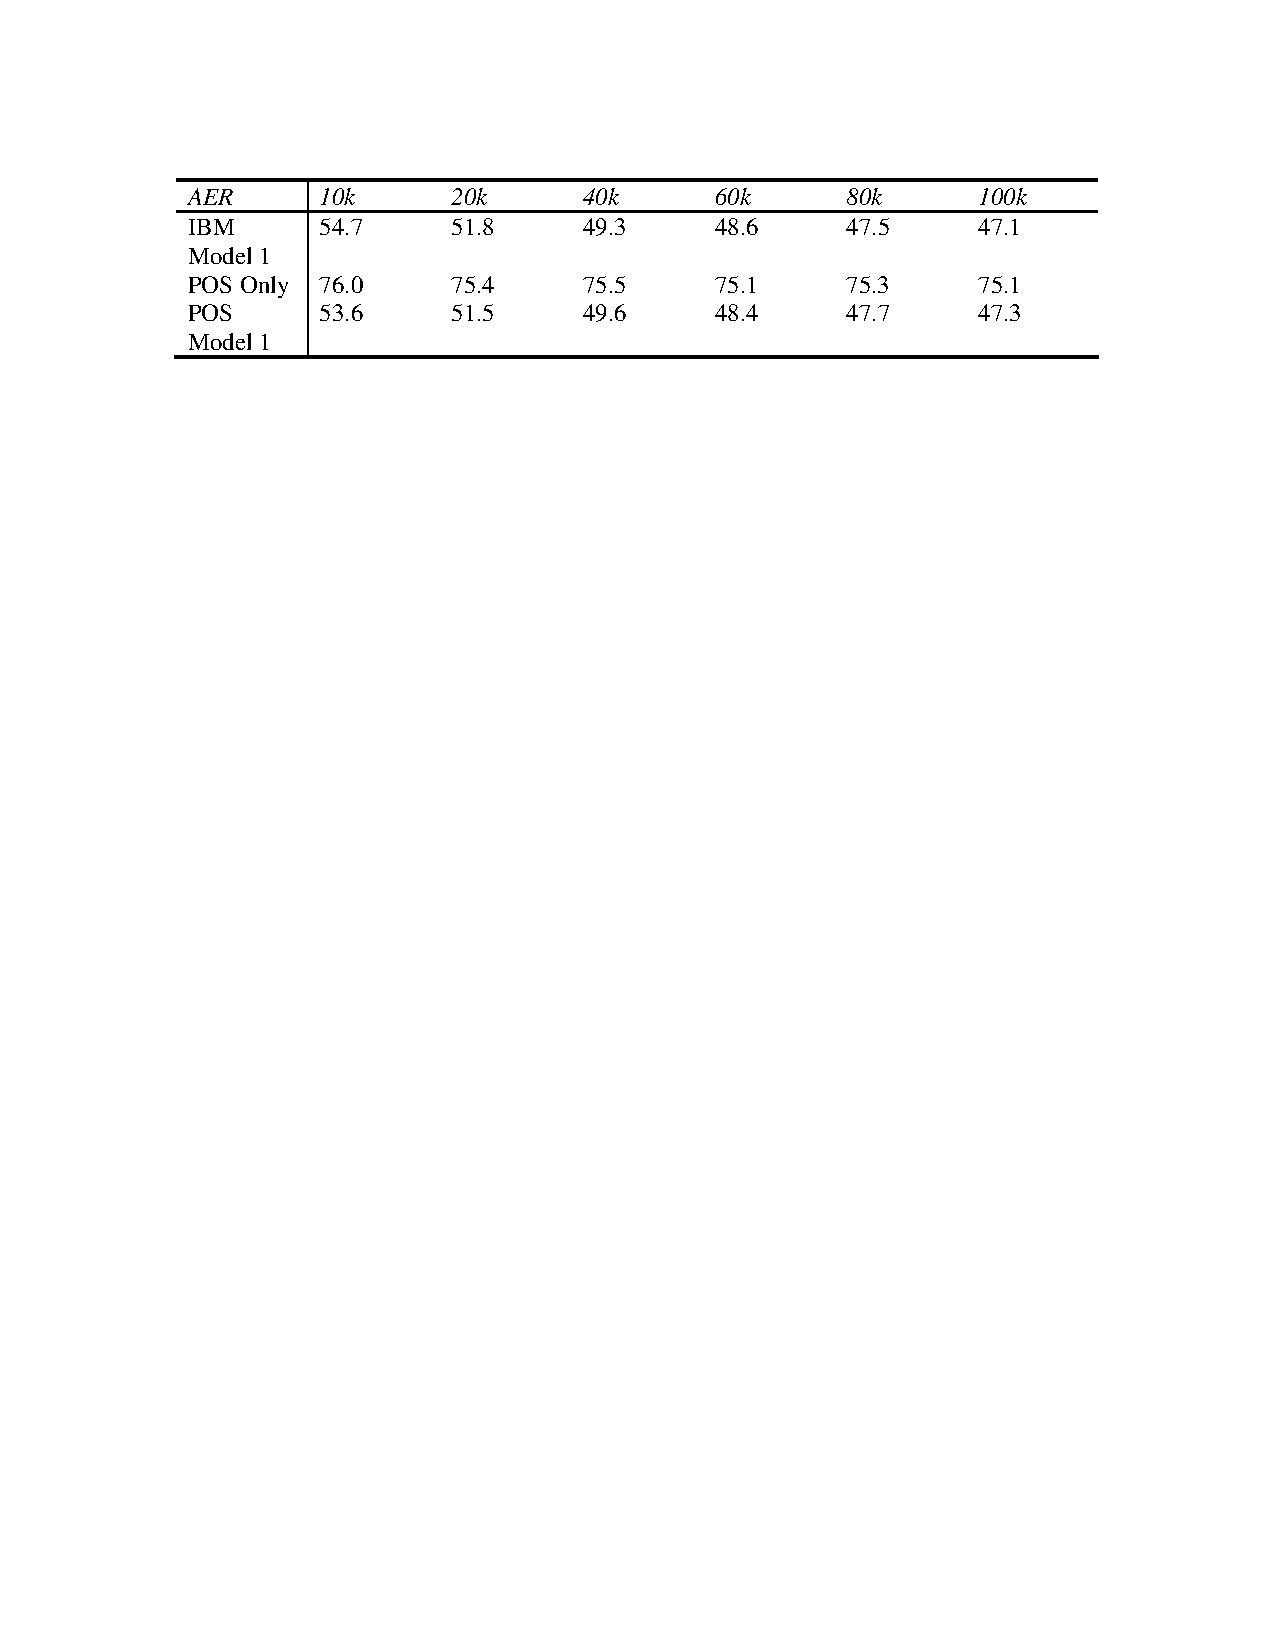
\includegraphics[scale=0.75,viewport = 90 600 510 730,clip]{constantin-table.pdf}
\end{center}

The first row indicates the number of sentences used for training
and the first column indicates the model used to generate
alignments.

As expected, the $AER$ of the alignments generated using only part
of speech information are very high, indicating that part-of-speech
information is not sufficient to generate good alignments. However,
an $AER$ of around $.75$ indicates that there is some information
provided by part-of-speech information that could be useful.

The $AER$ of alignments generated with IBM Model 1 doesn't
statistically differ from the $AER$ of alignments generated with the
additional part of speech information. One reason for this might be
that the part-of-speech probability was given equal weight to the
word probability, even though the latter is more important. POS
Model 2 might thus generate an improvement in $AER$.





\section{Distortion Models}\label{Christine's-project} %draft 0.01
Distortion modeling is  used as a feature function in our translation system adding in a score based on the likely placement of a phrase relative to an adjacent phrase. Two main forms of distortion modeling are used in contemporary state-of-the-art machine translation systems: distance distortion models, which penalize based on the distance of the reorder, and lexical distortion models, which take into account the relationship between the phrase being reordered and adjacent phrases. Moses extends lexical distortion models to factor distortion models, models in which lexical distortion serves as the special case using the surface forms as the factors in the probability distribution table.

\subsection{Distance Distortion Models}

Distance based distortion models consider the number of words over which the phrase is moved, as measured on the foreign side. An exponential penalty of $\delta^n$ for movements over n words is added \citep{koehn:05}. This distortion model has its limitations, especially in languages such as German and Japanese where reordering over greater distances is more common. Furthermore, some words are more acceptable to be reordered than others; for example an adjective such as ``white'' may often be reordered in a language in which adjectives appear in a different relative word order to English. A distance distortion model still offers a good starting point for distortion modeling; in fact, capping movement to approximately 4 words leads to BLEU score improvement, even in languages with relatively free word order \citep{koehn:05}.

\subsection{Lexical Distortion Models}

Many of the limitations of distance based distortion modeling are addressed in lexical distortion models \citep{tillmann:04, koehn:05}, which directly learn the probabilities for a given phrase being reordered relative to adjacent phrases. When collecting phrase pairs we can classify phrases as monotone, swap, or discontinuous based upon the relative placement of the phrases.\\
\indent $\bf{Monotone}$\\
\indent \indent Forward: word alignment point on bottom right\\
\indent \indent Backward: word alignment point on top left\\
\indent $\bf{Swap}$\\
\indent \indent Forward: word alignment point on bottom left\\
\indent \indent Backward: word alignment point on top right\\
\indent $\bf{Discontinuous}$\\
\indent \indent Not monotone or swap\\
Based upon this data, we calculate probability distributions of the form 
\begin{equation}
p_r(orientation|\bar{e},\bar{f})
\end{equation}
The design space for such a model is inherently larger, and three important design decisions are made in configuring the model, granularity of orientation distinction, side of the translation to condition the probability distribution on, and the directions of orientation to consider. Namely, one can distinguish between all three orientation classes or merely between monotone and non-monotone; one can condition the orientation probability distribution on the foreign phrase or on both the foreign and the source phrase; and one can model with respect to the previous phrase, the following phrase or both. Incorporating a lexical reordering model generally offers significant BLEU score improvements and the optimal configuration depends on language pair \citep{koehn:05}. Lexical reordering was analogously implemented in Moses, offering the significant gains in BLEU score detailed below.\\

\begin{tabular}{r|rrr}
Europarl Lang & Pharaoh & Moses\\ 
\hline
 En $\rightarrow$ De & 18.15 &18.85 \\ 
Es $\rightarrow$ En & 31.46 & 32.37 \\
En $\rightarrow$ Es &  31.06 & 31.85 \\
\end{tabular}
\subsection{Factor Distortion Models}
Hard-coding in a few factor based distortion rules to an existing statistical machine translation system, such as forcing the swap of nouns and adjectives when translating from English to Spanish, improves translation quality as measured by the BLEU score \citep{pop:06}. This is a motivating result for the development factor distortion models which statistically learn and apply such rules in an analogous manner to the lexical distortion model detailed above.

In factor distortion models we define a reordering model over an arbitrary subset of factors. For example, a part of speech factor distortion model has the ability to learn in a given language that the probability of an adjective being swapped with a noun is high, while the probability of an adjective being swapped with a verb is low. As compared with distance or lexical distortion models, generalizing through a factor distortion model makes better use of the available training data and more effectively models long range dependencies. If we encounter a surface form we have not seen before, we are more likely to handle it effectively through information obtained from its factors. In addition, t is more likely we will have seen a sequence of general factors corresponding to a phrase in our training data than the exact lexical surface form of the phrase itself. As such, by having longer phrases of factors in our training data we have access to reordering probabilities over a greater range, enabling us in turn to model reordering over a greater number of words.


\section{Error Analysis}\label{Evan's-project}
We describe some statistics generally used to measure error and present two error analysis tools written over the summer.

\subsection{Error Measurement}
There are three common measures of translation error. BiLingual Evaluation Understudy (BLEU) \citep{pop:06}, the most common, measures matches of short phrases between the translated and reference text as well as the difference in the lengths of the reference and output. BLEU can be applied to multiple references, but in a way such that BLEU scores using different numbers of references are not comparable.

Word Error Rate (WER) measures the number of matching output and reference words given that if output word $i$ is noted as matching reference word $j$, output word $i + 1$ cannot match any reference word before $j$; i.e., word ordering is preserved in both texts. Such a mapping isn't unique, so WER is specified using the maximum attainable number of single-word matches. This number is computable by some simple dynamic programming.

Position-Independent Word Error Rate (PWER) simply counts matching output and reference words regardless of their order in the text. This allows for rearrangement of logical units of text, but allows a system to get away with poor rearrangement of function words.

All these measures are highly dependent on the level of redundancy in the target language: the more reasonable translation options, the less likely the one chosen will match the reference exactly. So the scores we use are really comparable only for a specific source text in a specific language.

Perplexity (defined in \cite{perplexity}), measured for a text with respect to a language model, is a function of the likelihood of that text being produced by repeated application of the model. In a shaky sense, he higher the perplexity of a text, the more complex it is, so the harder it is to produce. The perplexity of the output of a modern machine translation system is usually lower (for our test case, by a factor of two to three) than that of a reliable reference translation. This is unsurprising because the people who provide the references have at their command long-range syntactic constructs that haven't been reconstructed via computer.

Along with these statistics, we'd like some assurance that they're stable, preferably in the form of confidence intervals. We use both the paired $t$ test and the more conservative sign test to obtain confidence intervals for the BLEU score of each translation system on a corpus.

All of these measures can be applied to a text of any size, but the larger the text, the more statistical these scores become. For detail about the kinds of errors a translation system is making, we need sentence-by-sentence error analysis. For this purpose we wrote two graphical tools.

\subsection{Tools}
As part of Koehn's PhD thesis, an online tool was developed that that keeps track of a set of corpuses (a corpus is a source text, at least one system output and at least one reference) and generates various statistics each time a corpus is added or changed. Before the workshop, his system showed BLEU scores and allowed a user to view individual sentences (source, output, reference) and score the output. For large numbers of sentences manual scoring isn't a good use of our time; the system was designed for small corpuses. To replace the manual-scoring feature we created a display of the BLEU scores in detail for each sentence: counts and graphical displays of matching n-grams of all sizes used by BLEU. See Figure~\ref{fig:sentence_by_sentence_screenshot} for screenshots.

The overall view for a corpus shows a list of files associated with a given corpus: a source text, one or more reference translations, one or more system translations. For the source it gives a count of unknown words in the source text (a measure of difficulty of translation, since we can't possibly correctly translate a word we don't recognize) and the perplexity. For each reference it shows perplexity. For each system output it shows WER and PWER, the difference between WER and PWER two for nouns and adjectives only (\cite{errMeasures}), the ratio of PWER of surface forms to PWER of lemmas (\cite{errMeasures}), and the results of some simple statistical tests, as described above, for the consistency of BLEU scores in different sections of the text. The system handles missing information decently, and shows the user a message to the effect that some measure is not computable. Also displayed are results of a $t$ test on BLEU scores between each pair of systems' outputs, which give the significance of the difference in BLEU scores of two systems on the same input.

A second tool developed during the workshop shows the mapping of individual source to output phrases (boxes of the same color on the two lines in Figure~\ref{fig:phrases_used_screenshot}) and gives the average source phrase length used. This statistic tells us how much use is being made of the translation model's capabilities. There's no need to take the time to tabulate all phrases of length 10, say, in the training source text if we're pretty sure that at translation time no source phrase longer than 4 words will be chosen.

\begin{figure}[h]
\centering
\frame{\vspace{.05in}\hspace{.05in}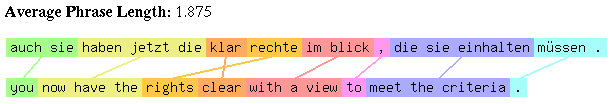
\includegraphics[width=5in]{images/show-phrases-used_crossover_screenshot.png}\hspace{.05in}\vspace{.05in}}
\caption{Sample output of phrase-detail tool.}
\label{fig:phrases_used_screenshot}
\end{figure}

\begin{figure}
\centering
%temp removed to encourage document to compile
{\bf Detailed view of sentences}\\
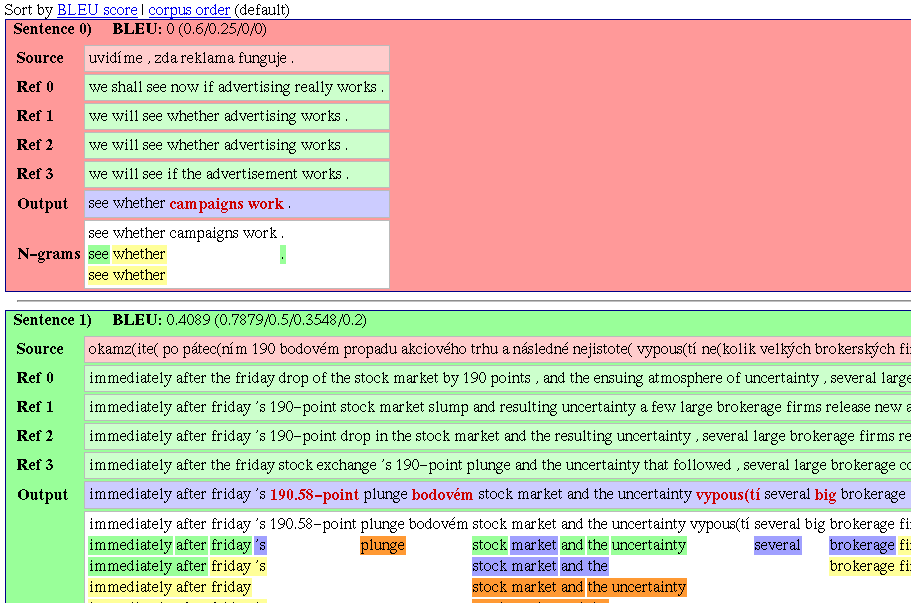
\includegraphics[width=6in]{images/sentence-by-sentence_multiref_screenshot.png}

\vspace{5mm}
{\bf Overall corpus view}
\includegraphics[width=6in]{images/corpus_overview_screenshot_de-en.png}
\caption{Sample output of corpus-statistics tool.}
\label{fig:sentence_by_sentence_screenshot}
\end{figure}











\end{document}
